%! TeX root = ../main.tex

%           TEMPLATE

%           \chapter{Spazi campionari}
%           
%           \ParteEsercizi
%           
%           \Esercizio{(Nome di un esercizio speciale)}
%           \Esercizio{}
%           \Esercizio{}
%           
%           \ParteSoluzioni
%           
%           \Soluzione
%           \Soluzione
%           \Soluzione
%           
%           
%           \chapter{Indipendenza}
%           
%           \ParteEsercizi
%           
%           \Esercizio{}
%           \begin{enumerate}
%               \item ine
%               \item oh
%               \item $\!\!\!\!{^*}$ jhk b
%           \end{enumerate}
%           \Esercizio{$*$}
%           \Esercizio{}
%           
%           \ParteSoluzioni
%           
%           \Soluzione
%           \Soluzione
%           \Soluzione









\chapter{Esercitazione 1 - Boella}
\ParteEsercizi
\Esercizio{}

Risolvere l'equazione
\begin{equation*}
\sin z=2
\end{equation*}
\Esercizio{}

Scrivere la serie di potenze di
\begin{equation*}
f(z)=\frac{1}{z^{2} -3z+2}
\end{equation*}
\Esercizio{}

Scrivere la serie di potenze di
\begin{equation*}
f(z)=\frac{e^{z}}{1+2z}
\end{equation*}
\Esercizio{}

La funzione
\begin{equation*}
u(x,y)=y^{3} -3x^{2} y
\end{equation*}
è armonica? Qual è la sua armonica coniugata?
\Esercizio{}

Calcolare $\int\nolimits _{\gamma _{1}} f(z)dz$ con
\begin{equation*}
f(z)=\overline{z} \ \ \ \ \gamma _{1} =\left( t,it^{2}\right) \ \ \ \ t\in [0,1]
\end{equation*}
\Esercizio{}

Calcolare $\int\nolimits _{\gamma _{1}} f(z)dz$ con
\begin{equation*}
f(z)=\overline{z} \ \ \ \ \gamma _{2} =(t,it)\ \ \ \ 
\end{equation*}
\Esercizio{}

Calcolare $\int _{\gamma _{1}} g(z)dz$ e $\int _{\gamma _{2}} g(z)dz$ con
\begin{equation*}
g(z)=z^{2} \ \ \ \ \gamma _{1} =\left( t,it^{2}\right) \ \ \ \ \gamma _{2} =(t,it)\ \ \ \ t\in [0,1]
\end{equation*}
\ParteSoluzioni
\Soluzione
\begin{theorem}
[Formule di Eulero] Il seno e il coseno complessi possono essere espressi come
\begin{equation*}
\sin z=\frac{e^{iz} -e^{-iz}}{2i} \ \ \cos z=\frac{e^{iz} +e^{-iz}}{2}
\end{equation*}
\end{theorem}
Si ha
\begin{align*}
\sin z=\frac{e^{iz} -e^{-iz}}{2i} & =2\\
e^{iz} -4i-e^{-iz} & =0\\
e^{2iz} -4ie^{iz} -1 & =0
\end{align*}
ponendo $w=e^{iz}$ abbiamo
\begin{equation*}
w^{2} -4iw-1=0\ \ \Rightarrow \ \ w=2i\pm \sqrt{3} i=(2\pm \sqrt{3} )i
\end{equation*}
Eguagliamo quindi
\begin{equation*}
(2\pm \sqrt{3} )i=e^{iz}
\end{equation*}
Ricordiamo che $z=x+iy$ e da ciò segue che
\begin{equation*}
e^{iz} =e^{ix-y} =e^{-y} e^{ix} \ \ \ \ \ \ \ \ (2\pm \sqrt{3} )i=(2\pm \sqrt{3} )e^{i\pi /2}
\end{equation*}
Uguagliando il modulo abbiamo
\begin{equation*}
e^{-y} =(2\pm \sqrt{3} )\ \ \Rightarrow \ \ y=-\ln (2\pm \sqrt{3} )
\end{equation*}
Uguagliando l'argomento abbiamo
\begin{equation*}
e^{ix} =e^{i\pi /2} \ \ \Rightarrow \ \ x=\frac{\pi }{2} +2k\pi 
\end{equation*}
L'equazione ha quindi \textit{infinite} soluzioni, date da infinite coppie di punti disposti su due rette parallele.
\Soluzione
\begin{definition}
La serie centra nel punto $z_{0}$ è data da
\begin{equation*}
\sum\limits ^{\infty }_{n=0} a_{n}\left( z-z_{0}\right)^{n}
\end{equation*}
\end{definition}
\begin{nb}
Il raggio di convergenza è $R$, ed è centrato in $z_{0}$. In tutti i punti interni la serie converge, nei punti esterni non converge, sulla circonferenza nulla si può dire in generale.
\end{nb}
\begin{theorem}
[Criterio del rapporto]
\begin{equation*}
\frac{1}{R} =\lim\limits _{n\rightarrow +\infty }\frac{\left| a_{n+1}\right| }{\left| a_{n}\right| }
\end{equation*}
Se il limite vale $\infty /0$, il raggio è $0/\infty $. Se il limite non esiste, il criterio fallisce.
\end{theorem}
\begin{theorem}
[Criterio della radice]
\begin{equation*}
\frac{1}{R} =\limsup\limits _{n\rightarrow \infty }\sqrt[n]{\left| a_{n}\right| }
\end{equation*}
Si noti che il limite superiore esiste sempre (a differenza del limite).
\end{theorem}
\begin{definition}
Serie prodotto secondo Cauchy
\begin{equation*}
A=\sum\limits ^{\infty }_{n=0} a_{n} ,\ \ B=\sum\limits ^{\infty }_{n=0} b_{n} \ \ \Rightarrow \ \ C=\sum\limits ^{\infty }_{n=0} a_{n}\sum\limits ^{\infty }_{n=0} b_{n} =\sum\limits ^{\infty }_{n=0} c_{n}
\end{equation*}
con
\begin{equation*}
c_{n} =\sum\limits ^{n}_{k=0} a_{k} b_{n-k}
\end{equation*}
\end{definition}
\begin{theorem}
La serie $C$ converge assolutamente ad $A\cdot B$, per il teorema di Mertens, se almeno una fra $A$ e $B$ converge assolutamente.

Se $A$ e $B$ hanno $R=+\infty ,$ si può ovviamente applicare il teorema di Mertens, e si può scrivere
\begin{equation*}
\sum\limits ^{\infty }_{n=0} a_{n}\sum\limits ^{\infty }_{n=0} b_{n} =\sum\limits ^{\infty }_{n,m=0} a_{n} b_{m}
\end{equation*}
\end{theorem}
\begin{nb}
[Serie notevoli]
\begin{align*}
e^{z} & =\sum ^{\infty }_{n=0}\frac{z^{n}}{n!} & R=+\infty \\
\cosh z & =\sum ^{\infty }_{n=0}\frac{z^{2n}}{(2n)!} & R=+\infty \\
\sinh z & =\sum ^{\infty }_{n=0}\frac{z^{2n+1}}{(2n+1)!} & R=+\infty \\
\cos z & =\sum ^{\infty }_{n=0}\frac{(-1)^{n} z^{2n}}{(2n)!} & R=+\infty \\
\sin z & =\sum ^{\infty }_{n=0}\frac{(-1)^{n} z^{2n+1}}{(2n+1)!} & R=+\infty \\
\frac{1}{1-z} & =\sum ^{\infty }_{n=0} z^{n} & R=1
\end{align*}
\end{nb}
Separiamo in due termini la frazione
\begin{equation*}
f(z)=\frac{1}{z^{2} -3z+2} =\frac{1}{( z-1)( z-2)} =\frac{1}{z-2} -\frac{1}{z-1} =\frac{1}{1-z} -\frac{1}{2-z}
\end{equation*}
Raccogliamo nel secondo termine
\begin{equation*}
\frac{1}{2-z} =\frac{\frac{1}{2}}{1-\frac{z}{2}} =\frac{1}{2}\frac{1}{1-\frac{z}{2}}
\end{equation*}
valgono poi
\begin{equation*}
\frac{1}{1-z} =\sum ^{\infty }_{n=0} z^{n} \ \ \ \ \frac{1}{2-z} =\frac{1}{2}\sum ^{\infty }_{n=0}\left(\frac{z}{2}\right)^{n} =\sum ^{\infty }_{n=0}\frac{1}{2^{n+1}} z^{n}
\end{equation*}
pertanto
\begin{equation*}
f(z)=\sum ^{\infty }_{n=0}\left( 1-\frac{1}{2^{n+1}}\right) z^{n}
\end{equation*}
Il raggio di convergenza è l'intersezione tra $|z|< 1$ e $|z|< 2$, ovvero $|z|< 1$.
\Soluzione
\begin{equation*}
f(z)=\frac{e^{z}}{1+2z} =e^{z} \cdotp \frac{1}{1-( -2z)} =( *)
\end{equation*}
Sviluppiamo in serie e scriviamo la serie prodotto secondo Cauchy
\begin{equation*}
( *) =\sum ^{\infty }_{n=0}\frac{z^{n}}{n!} \cdotp \sum ^{\infty }_{m=0} (-2z)^{m} =\sum ^{\infty }_{n=0}\sum ^{n}_{k=0}\frac{z^{k}}{k!} (-2)^{n-k} z^{n-k} =\sum ^{\infty }_{n=0}\left(\sum ^{n}_{k=0}\frac{(-2)^{n-k}}{k!}\right) z^{n}
\end{equation*}
In alternativa, sfruttando Mertens
\begin{equation*}
f(z)=\frac{e^{z}}{1+2z} =\sum ^{\infty }_{n=0}\frac{z^{n}}{n!} \cdotp \sum ^{\infty }_{n=0} (-2z)^{n} =\sum ^{\infty }_{n,m=0}\frac{z^{n}}{n!} (-2)^{m} z^{m}
\end{equation*}
\Soluzione
\begin{definition}
Una funzione si dice \textbf{armonica} se la somma delle sue derivate seconda è pari a zero.
\end{definition}
\begin{definition}
Una funzione si dice \textbf{olomorfa} se è derivabile in senso complesso.
\end{definition}
\begin{theorem}
Sia $f(z)$ olomorfa: $f(z)=f(x,y)=u(x,y)+iv(x,y)$. Allora $u$ e $v$ sono armoniche, e l'una è l'armonica coniugata dell'altra, secondo le condizioni di Cauchy-Riemann
\begin{equation*}
u_{x} =v_{y} \ \ \ \ u_{y} =-v_{x}
\end{equation*}
\end{theorem}
Deriviamo la funzione
\begin{gather*}
u_{x} =-6xy=v_{y}\\
u_{y} =3y^{2} -3x^{2} =-v_{x}
\end{gather*}
pertanto è armonica.

Integrando la $v_{x}$ abbiamo
\begin{equation*}
\int v_{x} dx=\int \left( 3x^{2} -3y^{2}\right) dx=x^{3} -3xy^{2} +h(y)
\end{equation*}
integrando la $v_{y}$ abbiamo
\begin{equation*}
\int v_{y} dy=\int -6xydy=-3xy^{2} +k(x)
\end{equation*}
Da ciò segue che $k(x)=x^{3}$ e $h(y)=\text{costante}$. Pertanto
\begin{equation*}
v(x,y)=x^{3} -3xy^{2}
\end{equation*}
e
\begin{align*}
f(z) & =f(x,y)\\
 & =u(x,y)+iv(x,y)\\
 & =\left( y^{3} -3x^{2} y\right) +i\left( x^{3} -3xy^{2}\right)\\
 & =iz^{3}
\end{align*}
\Soluzione

È noto che
\begin{equation*}
f(z)=\overline{z} =x-iy\ \ \ \ dz=d\left( t+it^{2}\right) =dt+2itdt=\left( 1+2it\right) dt
\end{equation*}
Pertanto
\begin{align*}
\int _{\gamma _{1}} f(z)dz & =\int ^{1}_{0}\left( t-it^{2}\right) (1+2it)dt\\
 & =\int ^{1}_{0}\left( t+it^{2} +2t^{3}\right) dt\\
 & =\left[\frac{t^{2}}{2} +i\frac{t^{3}}{3} +\frac{t^{4}}{2}\right]^{1}_{0}\\
 & =1+\frac{i}{3}
\end{align*}
\Soluzione

È noto che
\begin{gather*}
f(z)=\overline{z} =x-iy\\
dz=dx+idy\\
dx=dt\\
dy=dt
\end{gather*}
Pertanto
\begin{equation*}
\int _{\gamma _{2}} f(z)dz=\int ^{1}_{0} (t-it)(1+i)dt=\int ^{1}_{0} 2tdt=1
\end{equation*}
Notiamo che l'integrale dipende dal percorso scelto, essendo $\overline{z}$ una funzione \textit{non} olomorfa.
\Soluzione

Osserviamo che
\begin{gather*}
z^{2} =x^{2} -y^{2} +2ixy\\
dx+idy=dt+2itdt
\end{gather*}
Pertanto
\begin{align*}
\int _{\gamma _{1}} g(z)dz & =\int ^{1}_{0}\left( t^{2} -t^{4} +2it^{3}\right) (1+2it)dt\\
 & =\left[\frac{t^{3}}{3} +it^{4} -5t^{5} -\frac{i}{3} t^{6}\right]^{1}_{0}\\
 & =-\frac{2}{3} +\frac{2}{3} i
\end{align*}
\textit{Esercizio:} svolgere l'integrale $\gamma _{2}$, spiegando perché ora il risultato sia uguale.
\chapter{Esercitazione 1 - Potrich}
\ParteEsercizi
\Esercizio{}

Determinare in quali punti del piano complesso la funzione
\begin{equation*}
f\left( z\right) =z^{2}\left| z\right| ^{2} e^{i\overline{z}^{2}}
\end{equation*}
è derivabile in senso complesso.
\Esercizio{}

Mostrare che
\begin{equation*}
u\left( x,y\right) =2x-2xy
\end{equation*}
è armonica e trovare la sua armonica coniugata.
\Esercizio{}

Sia $\gamma \left( t\right) =t+it^{2} ,t\in \left[ -1,0\right]$. Calcolare
\begin{equation*}
\int\nolimits _{\gamma }\left[\overline{z} +\left( z+1\right)^{7}\right] dz
\end{equation*}
\Esercizio{}

Calcolare
\begin{equation*}
\int\nolimits _{\gamma }\left(\overline{z}\right)^{2} dz
\end{equation*}
dove $\gamma $ è la circonferenza centrata in $z=1$ e raggio unitario percorsa in senso antiorario.
\Esercizio{}

Risolvere
\begin{equation*}
\sin z=3
\end{equation*}
\Esercizio{}

Calcolare la somma della serie
\begin{equation*}
\sum\limits ^{\infty }_{n=1}\left( 3n+7\right) z^{n}
\end{equation*}
all'interno del suo disco di convergenza.
\ParteSoluzioni
\Soluzione
\begin{definition}
Siano $\Omega \subseteq \mathbb{C}$, $f:\Omega \rightarrow \mathbb{C}$ è derivabile, in senso complesso, in $z_{0}$ se $\exists $ finito
\begin{equation*}
\lim\limits _{h\rightarrow 0}\frac{f\left( z_{0} +h\right) -f\left( z_{0}\right)}{h} ,\ \ \ \ h\in \mathbb{C}
\end{equation*}
\end{definition}
\begin{definition}
Sia $\Omega \in \mathbb{C}$ aperto. Se $f$ è derivabile in ogni punto di $\Omega $, allora $f$ è \textbf{olomorfa} in $\Omega $, $f\in \mathcal{H}\left( \Omega \right)$.
\end{definition}
\begin{nb}
Se $\Omega \equiv \mathbb{C}$ allora $f$ è \textbf{intera}.
\end{nb}
\begin{theorem}
[di Cauchy-Riemann] Sia $\Omega \subseteq \mathbb{C}$ aperto, $f:\Omega \rightarrow \mathbb{C}$ definita come
\begin{equation*}
f\left( z\right) =u\left( x,y\right) +iv\left( x,y\right) =\mathrm{Re}\left( z\right) +i\mathrm{Im}\left( z\right)
\end{equation*}
è olomorfa in $\Omega $ se e solo se $u,v:\Omega \rightarrow \mathbb{R}$ sono differenziabili in senso classico in $\Omega $ e valgono le \textbf{condizioni di Cauchy-Riemann}
\begin{equation}
\begin{cases}
u_{x}\left( x,y\right) =v_{y}\left( x,y\right)\\
u_{y}\left( x,y\right) =-v_{x}\left( x,y\right)
\end{cases}
\end{equation}
\end{theorem}
\begin{obs}
Un altro modo per scrivere le (1) è
\begin{equation*}
\frac{\partial f}{\partial \overline{z}} =0
\end{equation*}
Infatti
\begin{equation*}
\begin{array}{ l }
x=\mathrm{Re}\left( z\right) =\frac{z+\overline{z}}{2}\\
y=\mathrm{Im}\left( z\right) =-i\frac{z-\overline{z}}{2}
\end{array}
\end{equation*}
allora
\begin{equation*}
f\left( x,y\right) =f\left(\frac{z+\overline{z}}{2} ,-i\frac{z-\overline{z}}{2}\right)
\end{equation*}
Per la regola della catena
\begin{equation*}
\frac{\partial f}{\partial \overline{z}} =\frac{1}{2}\left(\frac{\partial f}{\partial x} +i\frac{\partial f}{\partial y}\right) =0
\end{equation*}
che vale in quanto
\begin{equation*}
\begin{cases}
f_{x} =f'=u_{x} +iv_{x} =v_{y} -iu_{y}\\
f_{y} =if'=iu_{x} -v_{x} =iv_{y} +u_{y}
\end{cases}
\end{equation*}
\end{obs}
Poniamo $z=x+iy$
\begin{align*}
f\left( z\right) & =\left( x+iy\right)^{2}\left( x^{2} +y^{2}\right) e^{i\left( x-iy\right)^{2}}\\
 & =\left( x+iy\right)^{2}\left( x^{2} +y^{2}\right) e^{i\left( x^{2} -y^{2} -2ixy\right)}\\
 & =\left( x^{2} -y^{2} +2ixy\right)\left( x^{2} +y^{2}\right) e^{2xy+i\left( x^{2} -y^{2}\right)}\\
 & =\left( x^{2} -y^{2} +2ixy\right)\left( x^{2} +y^{2}\right) e^{2xy}\left[\cos\left( x^{2} -y^{2}\right) +i\sin\left( x^{2} -y^{2}\right)\right]\\
 & =\left( x^{2} +y^{2}\right) e^{2xy}\left[\left( x^{2} -y^{2}\right)\cos\left( x^{2} -y^{2}\right) -2xy\sin\left( x^{2} -y^{2}\right)\right]\\
 & +i\left( x^{2} +y^{2}\right) e^{2xy}\left[ 2xy\cos\left( x^{2} -y^{2}\right) +\left( x^{2} -y^{2}\right)\sin\left( x^{2} -y^{2}\right)\right]
\end{align*}
$u,v\in C^{1}\left(\mathbb{R}^{2}\right)$.

Osserviamo che $f\left( z\right) =z^{2} \cdotp z\overline{z} \cdotp e^{i\overline{z}^{2}} =z^{3}\overline{z} e^{i\overline{z}^{2}}$
\begin{align*}
\frac{\partial f}{\partial \overline{z}} & =z^{3} e^{i\overline{z}^{2}} +z^{3}\overline{z} 2i\overline{z} e^{i\overline{z}^{2}}\\
 & =z^{3} e^{i\overline{z}^{2}}\left( 1+2i\overline{z}^{2}\right) =0
\end{align*}
Notiamo intanto che $z_{1} =0$ è soluzione.
\begin{equation*}
1+2i\overline{z}^{2} =0\ \ \Rightarrow \ \ \overline{z}^{2} =-\frac{1}{2i} =\frac{i}{2}
\end{equation*}
Scrivendo $\overline{z} =x-iy$ abbiamo
\begin{gather*}
\begin{aligned}
\left( x-iy\right)^{2} & =\frac{i}{2}\\
x^{2} -y^{2} -2ixy & =\frac{i}{2}
\end{aligned}\\
\Downarrow \\
\begin{cases}
x^{2} -y^{2} =0\\
-2xy=\frac{1}{2}
\end{cases} \ \ \Rightarrow \ \ \begin{cases}
x^{2} -\frac{1}{16x^{2}} =0\\
y=-\frac{1}{4x}
\end{cases} \ \ \Rightarrow \ \ \begin{cases}
16x^{4} -1=0\\
y=-\frac{1}{4x}
\end{cases}
\end{gather*}
Le cui soluzioni sono
\begin{gather*}
x_{2} =\frac{1}{2} \ \ \rightarrow \ \ y_{2} =-\frac{1}{2} \ \ \rightarrow \ \ z_{2} =\frac{1}{2} -\frac{i}{2}\\
x_{3} =-\frac{1}{2} \ \ \rightarrow \ \ y_{3} =\frac{1}{2} \ \ \rightarrow \ \ z_{3} =-\frac{1}{2} +\frac{i}{2}
\end{gather*}
\Soluzione
\begin{definition}
Le condizioni che verificano l'armonicità di $u$ sono
\begin{equation}
u\in C^{2}\left(\mathbb{R}^{2}\right) ,\ \Delta u=u_{xx} +u_{yy} =0
\end{equation}
\end{definition}
La prima è certamente vera, controlliamo che il laplaciano di $u$ sia nullo
\begin{equation*}
\begin{array}{ r }
u_{x} =2-2y\ \ \rightarrow \ \ u_{xx} =0\\
u_{y} =-2x\ \ \rightarrow \ \ u_{yy} =0
\end{array} \ \ \Rightarrow \ \ \Delta u=0
\end{equation*}
deduciamo che $u$ è armonica. Trovare la funzione armonica coniugata di $u$ equivale a trovare una funzione armonica $v$ tale che $u,v$ soddisfano le condizioni di Cauchy-Riemann.
\begin{equation*}
\begin{cases}
u_{x} =v_{y}\\
u_{y} =-v_{x}
\end{cases} \ \ \Rightarrow \ \ \begin{cases}
2-2y=v_{y}\\
-2x=-v_{x}
\end{cases} \ \ \Rightarrow \ \ v\left( x,y\right) =x^{2} -y^{2} +2y+c,\ \ c\in \mathbb{R}
\end{equation*}
\Soluzione
\begin{definition}
Sia $\Omega \subseteq \mathbb{C}$ aperto, $f:\Omega \rightarrow \mathbb{C}$ continua in $\Omega $, $\gamma :\left[ a,b\right]\rightarrow \Omega $ una curva $C^{1}$ a tratti, allora
\begin{equation*}
\int\nolimits _{\gamma } f\left( z\right) dz=\int\nolimits ^{b}_{a} f\left( \gamma \left( t\right)\right) \gamma '\left( t\right) dt
\end{equation*}
dove
\begin{gather*}
\gamma \left( t\right) =x\left( t\right) +iy\left( t\right)\\
\gamma '\left( t\right) =x'\left( t\right) +iy'\left( t\right)
\end{gather*}
\end{definition}
\begin{obs}
L'integrale curvilineo dipende dall'orientazione di $\gamma $
\begin{equation*}
\int\nolimits _{-\gamma } f\left( z\right) dz=-\int\nolimits _{\gamma } f\left( z\right) dz
\end{equation*}
\end{obs}
\begin{theorem}
Sia $\Omega \subseteq \mathbb{C}$ aperto, $f:\Omega \rightarrow \mathbb{C}$ continua. TFAE (the followings are equivalent):

1) $\int _{\gamma } f\left( z\right) dz$ dipende solo dagli estremi di $\gamma $

2) $\forall \gamma $ chiusa $C^{1}$ a tratti si ha $\int _{\gamma } f\left( z\right) dz=0$

3) $\exists F\in \mathcal{H}\left( \Omega \right) \cap C^{1}\left( \Omega \right)$ tale che $F'=f$ in $\Omega $
\end{theorem}
\textbf{\underline{1 modo}}
\begin{align*}
\int\nolimits _{\gamma }\left[\overline{z} +\left( z+1\right)^{7}\right] dz & =\int\nolimits ^{0}_{-1}\underbrace{\left[\left( t-it^{2}\right) +\left( t+it^{2} +1\right)^{7}\right]}_{f\left( \gamma \left( t\right)\right)}\underbrace{\left( 1+2it\right)}_{\gamma '\left( t\right)} dt\\
 & =\int\nolimits ^{0}_{-1}\left[\left( t+2it^{2} -it^{2} +2t^{3}\right) +\left( t+it^{2} +1\right)^{7}\left( 1+2it\right)\right] dt\\
 & =\int\nolimits ^{0}_{-1}\left[\left( t+it^{2} +2t^{3}\right) +\left( t+it^{2} +1\right)^{7}\left( 1+2it\right)\right] dt\\
 & =\left[\frac{t^{2}}{2} +i\frac{t^{3}}{3} +\frac{t^{4}}{2} +\frac{\left( t+it^{2} +1\right)^{8}}{8}\right]^{0}_{-1}\\
 & =\cancel{\frac{1}{8}} -\left\{\frac{1}{2} -\frac{i}{3} +\frac{1}{2} +\cancel{\frac{1}{8}}\right\} =-1+\frac{i}{3}
\end{align*}
\begin{nb}
$\overline{z}$ non è olomorfa
\begin{align*}
\lim\limits _{h\rightarrow 0}\frac{f\left( z_{0} +h\right) -f\left( z_{0}\right)}{h} & =\lim\limits _{h\rightarrow 0}\frac{\overline{z_{0} +h} -\overline{z_{0}}}{h}\\
 & =\lim\limits _{h\rightarrow 0}\frac{\cancel{\overline{z_{0}}} +\overline{h} -\cancel{\overline{z_{0}}}}{h}
\end{align*}
non esiste finito. Intuiamo che anche $\left| z\right| ^{2} =z\overline{z}$ avrà problemi. In particolare si dimostra che $\left| z\right| ^{2}$ è derivabile in senso complesso solo nell'origine. Il suo analogo in $\mathbb{R}^{2}$ sarebbe $f\left( x,y\right) =x^{2} +y^{2}$, che però è derivabile ovunque.
\end{nb}
\textbf{\underline{2 modo}}

Consideriamo le due parti di $f\left( z\right)$
\begin{equation*}
f\left( z\right) =\overline{z} +\left( z+1\right)^{7} =g\left( z\right) +h\left( z\right)
\end{equation*}
dove
\begin{equation*}
\begin{aligned}
g\left( z\right) =\overline{z} & \notin \mathcal{H}\left( \Omega \right)\\
h\left( z\right) =\left( z+1\right)^{7} & \in \mathcal{H}\left( \Omega \right)
\end{aligned}
\end{equation*}
La funzione $H\left( z\right) =\frac{\left( z+1\right)^{8}}{8}$ è tale che $H'\left( z\right) =h\left( z\right)$, quindi per il teorema visto l'integrale dipende solo dagli estremi
\begin{equation*}
\int\nolimits _{\gamma } f\left( z\right) dz=\int\nolimits _{\gamma }\overline{z} dz+\underbrace{H\left( \gamma \left( 0\right)\right) -H\left( \gamma \left( 1\right)\right)}_{\int\nolimits _{\gamma }\left( z+1\right)^{7} dz} =\dotsc 
\end{equation*}
\Soluzione

Scriviamo una possibile parametrizzazione della curva
\begin{equation*}
\gamma \left( t\right) =1+e^{it} ,\ \ t\in \left[ 0,2\pi \right]
\end{equation*}
e calcoliamo
\begin{align*}
\int\nolimits _{\gamma }\left(\overline{z}\right)^{2} dz & =\int\nolimits ^{2\pi }_{0}\left(\overline{1+e^{it}}\right)^{2} ie^{it} dt\\
 & =\int\nolimits ^{2\pi }_{0}\left( 1+e^{-it}\right)^{2} ie^{it} dt\\
 & =\int\nolimits ^{2\pi }_{0}\left( 1+2e^{-it} +e^{-2it}\right) ie^{it} dt\\
 & =i\int\nolimits ^{2\pi }_{0}\left( e^{it} +2+e^{-it}\right) dt\\
 & =\left[ e^{it} +2it-e^{it}\right]^{2\pi }_{0} =4\pi i
\end{align*}
\textit{Domanda:} $f\left( z\right) =\left(\overline{z}\right)^{2}$ ammette primitiva in un qualsiasi dominio $D$ contenente $\gamma $? No, se per assurdo la ammettesse, allora ogni integrale lungo qualsiasi curva chiusa sarebbe nullo.
\Soluzione

Ragioniamo come segue
\begin{align*}
\frac{e^{iz} -e^{-iz}}{2i} & =3\\
e^{iz} -e^{-iz} & =6i\\
e^{iz} -\frac{1}{e^{iz}} -6i & =0\\
e^{2iz} -6ie^{iz} -1 & =0\\
e^{iz} & =3i\pm 2\sqrt{2} i=\left( 3\pm 2\sqrt{2}\right) i
\end{align*}
Risolviamo per $z$
\begin{align*}
iz_{k} & =\log\left[\left( 3\pm 2\sqrt{2}\right) i\right]\\
 & =\ln\left| \left( 3\pm 2\sqrt{2}\right) i\right| +i\arg\left[\left( 3\pm 2\sqrt{2}\right) i\right]\\
 & =\ln\left| 3\pm 2\sqrt{2}\right| +i\left(\frac{\pi }{2} +2k\pi \right) ,\ \ \ \ k\in \mathbb{Z}
\end{align*}
Allora
\begin{equation*}
z_{k} =-i\ln\left| 3\pm 2\sqrt{2}\right| +\left(\frac{\pi }{2} +2k\pi \right) ,\ \ \ \ k\in \mathbb{Z}
\end{equation*}
Che può essere facilmente rappresentato nel piano di Gauss come un insieme di punti.
\Soluzione

Utilizziamo il criterio del rapporto per determinare $R$
\begin{equation*}
\frac{\left| a_{n+1}\right| }{\left| a_{n}\right| } =\frac{3\left( n+1\right) +7}{3n+7}\xrightarrow{n\rightarrow \infty } 1=\frac{1}{R}
\end{equation*}
Il raggio di convergenza è $R=1$.

La serie converge assolutamente $\forall z\in \mathbb{C} :\left| z\right| < 1$ e non converge per $\left| z\right|  >1$. Se $\left| z\right| =1$ la serie non converge perché il suo termine generale non tende a $0$. Per ogni $z\in \mathbb{C} :\left| z\right| < 1$ si ha
\begin{align*}
\sum\limits ^{\infty }_{n=1}\left( 3n+7\right) z^{n} & =3\sum\limits ^{\infty }_{n=1} nz^{n} +7\sum\limits ^{\infty }_{n=1} z^{n}\\
 & =3z\sum\limits ^{\infty }_{n=1} nz^{n-1} +7\sum\limits ^{\infty }_{n=1} z^{n}\\
 & =3z\sum\limits ^{\infty }_{n=1}\frac{d}{dz} z^{n} +7\sum\limits ^{\infty }_{n=1} z^{n}\\
 & =3z\frac{d}{dz}\sum\limits ^{\infty }_{n=1} z^{n} +7\sum\limits ^{\infty }_{n=1} z^{n}\\
 & =3z\frac{d}{dz}\left(\frac{1}{1-z} -1\right) +7\left(\frac{1}{1-z} -1\right)\\
 & =\frac{3z}{\left( 1-z\right)^{2}} +\frac{7}{1-z} -7
\end{align*}
\chapter{Esercitazione 2 - Boella}
\ParteEsercizi
\Esercizio{}

Scrivere la serie di potenze di
\begin{equation*}
f\left( z\right) =\frac{1}{1-z} -\frac{1}{2-z}
\end{equation*}
\Esercizio{}

Scrivere la serie di potenze di
\begin{equation*}
f\left( z\right) =z^{3}\sin\frac{1}{z}
\end{equation*}
\Esercizio{}

Classificare le singolarità di
\begin{equation*}
f\left( z\right) =\frac{z^{2}}{\sin z}
\end{equation*}
\Esercizio{}

Classificare le singolarità di
\begin{equation*}
f\left( z\right) =\frac{z^{2}}{\cos^{2}\left(\frac{1}{z}\right)}
\end{equation*}
\Esercizio{}

Classificare le singolarità di
\begin{equation*}
f\left( z\right) =\frac{e^{1/z}}{1+z^{2}}
\end{equation*}
\Esercizio{(Integrale di Fresnel)}

Calcolare
\begin{equation*}
\int ^{+\infty }_{0}\cos x^{2} dx
\end{equation*}
\ParteSoluzioni
\Soluzione

Osserviamo che ha singolarità in $1$ e $2$, che sono due poli di ordine $1$.
\begin{align*}
f\left( z\right) & =\frac{1}{1-z} -\frac{1}{2-z}\\
 & =\frac{1}{1-z} -\frac{1}{2}\frac{1}{1-\frac{z}{2}}\\
 & =\sum\limits ^{\infty }_{n=0} z^{n} -\frac{1}{2}\sum\limits ^{\infty }_{n=0}\frac{1}{2^{n}} z^{n}\\
 & =\sum\limits ^{\infty }_{n=0}\left( 1-\frac{1}{2^{n+1}}\right) z^{n}
\end{align*}
Manipoliamola in modo diverso
\begin{align*}
f\left( z\right) & =-\frac{1}{z} \cdotp \frac{1}{1-\frac{1}{z}} -\frac{1}{2}\frac{1}{1-\frac{z}{2}}\\
 & =-\frac{1}{z}\sum\limits ^{\infty }_{n=0} z^{-n} -\frac{1}{2}\sum\limits ^{\infty }_{n=0}\frac{z^{n}}{2^{n}}\\
 & =-\sum\limits ^{-1}_{n=-\infty } z^{n} -\sum\limits ^{\infty }_{n=0}\frac{z^{n}}{2^{n+1}}
\end{align*}
Le due serie convergono per
\begin{equation*}
1< \left| z\right| < 2
\end{equation*}
\Soluzione
\begin{align*}
f\left( z\right) & =z^{3}\sin\frac{1}{z}\\
 & =z^{3}\sum\limits ^{\infty }_{n=0}\frac{\left( -1\right)^{n}}{\left( 2n+1\right) !}\left(\frac{1}{z}\right)^{2n+1}\\
 & =\sum\limits ^{\infty }_{n=0}\frac{\left( -1\right)^{n}}{\left( 2n+1\right) !} z^{2-2n}\\
 & =z^{2} -\frac{1}{3!} +\frac{1}{5!z^{2}}
\end{align*}
Ha singolarità in $z=0$ di tipo essenziale (ci sono infinite potenze negative nello sviluppo). Il raggio di convergenza è $R=+\infty $. Il residuo nell'origine è $0$ (è il coefficiente $a_{-1}$ dello sviluppo). All'infinito la funzione si comporta come $z^{2}$. Il punto all'infinito è un polo di ordine $2$. Lo sviluppo vale sia all'infinito che nell'origine.
\Soluzione

I punti singolari sono
\begin{equation*}
z=k\pi ,\ \ k\in \mathbb{Z}
\end{equation*}
In particolare
\begin{itemize}
\item $z=0$ è una singolarità eliminabile, perché annulla sia il denominatore che il numeratore, quindi ha residuo nullo.\footnote{L'implicazione \textit{singolarità eliminabile} allora \textit{residuo nullo} vale solo per i \textbf{punti finiti}, non per il punto all'infinito.}
\item $z=k\pi $ sono poli del I ordine, $k\in \mathbb{Z} ,k\neq 0$, il cui residuo vale\begin{equation*}
\mathrm{Res}\left( f,k\pi \right) =\frac{g\left( k\pi \right)}{h'\left( k\pi \right)} =\frac{\left( k\pi \right)^{2}}{\left(\sin k\pi \right) '} =\frac{\left( k\pi \right)^{2}}{\cos k\pi } =\frac{\left( k\pi \right)^{2}}{\left( -1\right)^{k}}
\end{equation*}
\item $z_{\infty }$ è una singolarità non isolata perché non esiste un raggio che contiene tutti i punti singolari. Andando all'infinito avremo infiniti punti singolari.
\end{itemize}
\Soluzione

I punti di singolarità sono dati da
\begin{equation*}
\frac{1}{z_{k}} =\frac{\pi }{2} +k\pi \ \ \ \ k\in \mathbb{Z} \ \ \ \ \Rightarrow \ \ \ \ z_{k} =\frac{1}{\pi \left(\frac{1}{2} +k\right)}
\end{equation*}
Sono poli del II ordine perché il coseno qui si annulla con ordine $2$. In $z=0$ è una singolarità non isolata dato che gli $z_{k}$ si addensano intorno a $0$. Il punto $z_{\infty }$ è un polo di ordine II perché per $z\rightarrow z_{\infty } ,f\left( z\right) \sim z^{2}$.
\Soluzione

Il denominatore si annulla in $z=\pm i$, con un polo di ordine $1$. Ricordando
\begin{equation*}
e^{1/z} =\sum\limits ^{\infty }_{n=0}\frac{1}{n!}\left(\frac{1}{z}\right)^{n} =\sum\limits ^{\infty }_{n=0}\frac{1}{n!} z^{-n}
\end{equation*}
deduciamo che nell'origine si ha una singolarità essenziale. Si ha poi
\begin{align*}
f\left( z\right) & =\sum\limits ^{\infty }_{n=0}\frac{1}{n!} z^{-n}\sum\limits ^{\infty }_{m=0}\left( -1\right)^{m} z^{2m} =\sum\limits ^{\infty }_{n,m=0}\frac{\left( -1\right)^{m}}{n!} z^{2m-n}
\end{align*}
che converge per $\left| z\right| < 1$. Il residuo vale
\begin{equation*}
a_{-1} =\sum\limits ^{\infty }_{m=0,n=2m+1}\frac{\left( -1\right)^{m}}{n!} =\sum\limits ^{\infty }_{m=0}\frac{\left( -1\right)^{m}}{\left( 2m+1\right) !} =\sin 1
\end{equation*}
\Soluzione

Consideriamo $f\left( z\right) =e^{iz^{2}}$ e $\gamma =\gamma _{1} +\gamma _{2} +\gamma _{3}$


\begin{figure}[htpb]
	\centering
\tikzset{every picture/.style={line width=0.75pt}} %set default line width to 0.75pt        

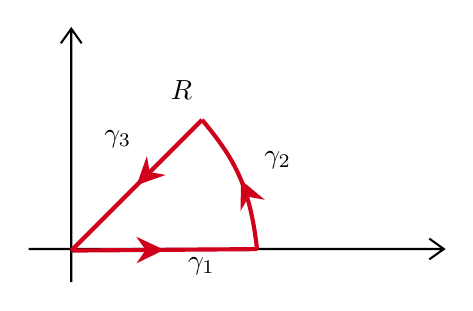
\begin{tikzpicture}[x=0.75pt,y=0.75pt,yscale=-1,xscale=1]
%uncomment if require: \path (0,176); %set diagram left start at 0, and has height of 176

%Shape: Axis 2D [id:dp035634818552425784] 
\draw  (200,140.05) -- (400,140.05)(220.5,33.92) -- (220.5,156) (393,135.05) -- (400,140.05) -- (393,145.05) (215.5,40.92) -- (220.5,33.92) -- (225.5,40.92)  ;
%Straight Lines [id:da7560460514537715] 
\draw [color={rgb, 255:red, 208; green, 2; blue, 27 }  ,draw opacity=1 ][line width=1.5]    (220.5,140.8) -- (283.5,77.8) ;
\draw [shift={(252,109.3)}, rotate = 315] [fill={rgb, 255:red, 208; green, 2; blue, 27 }  ,fill opacity=1 ][line width=0.08]  [draw opacity=0] (13.4,-6.43) -- (0,0) -- (13.4,6.44) -- (8.9,0) -- cycle    ;
%Curve Lines [id:da9635953000928117] 
\draw [color={rgb, 255:red, 208; green, 2; blue, 27 }  ,draw opacity=1 ][line width=1.5]    (283.5,77.8) .. controls (298.5,95.8) and (306.5,108.8) .. (310,140.11) ;
\draw [shift={(302.31,106.84)}, rotate = 65.41] [fill={rgb, 255:red, 208; green, 2; blue, 27 }  ,fill opacity=1 ][line width=0.08]  [draw opacity=0] (13.4,-6.43) -- (0,0) -- (13.4,6.44) -- (8.9,0) -- cycle    ;
%Straight Lines [id:da9987973908776102] 
\draw [color={rgb, 255:red, 208; green, 2; blue, 27 }  ,draw opacity=1 ][line width=1.5]    (220.5,140.8) -- (310,140.11) ;
\draw [shift={(265.25,140.45)}, rotate = 539.56] [fill={rgb, 255:red, 208; green, 2; blue, 27 }  ,fill opacity=1 ][line width=0.08]  [draw opacity=0] (13.4,-6.43) -- (0,0) -- (13.4,6.44) -- (8.9,0) -- cycle    ;

% Text Node
\draw (235,81.4) node [anchor=north west][inner sep=0.75pt]    {$\gamma _{3}$};
% Text Node
\draw (312,91.4) node [anchor=north west][inner sep=0.75pt]    {$\gamma _{2}$};
% Text Node
\draw (275.25,142.85) node [anchor=north west][inner sep=0.75pt]    {$\gamma _{1}$};
% Text Node
\draw (267,57.4) node [anchor=north west][inner sep=0.75pt]    {$R$};


\end{tikzpicture}
\end{figure}
\FloatBarrier

La funzione $f\left( z\right)$ è olomorfa, allora
\begin{equation*}
{\displaystyle \int\nolimits _{\gamma } f\left( z\right) dz=0=\int\nolimits _{\gamma _{1}} f\left( z\right) dz+\int\nolimits _{\gamma _{2}} f\left( z\right) dz+\int\nolimits _{\gamma _{3}} f}\left( z\right) dz
\end{equation*}
\begin{itemize}
\item La curva $\gamma _{3}$ ha parametrizzazione $z=re^{i\vartheta }$ con $r$ variabile e $\vartheta $ fissato. Il valore di $\vartheta $ si determina imponendo di potersi ricondurre all'integrale di Gauss, ovvero\begin{equation*}
iz^{2} =i\left( re^{i\vartheta }\right)^{2} =-r^{2} \ \ \Rightarrow \ \ \vartheta =\frac{\pi }{4}
\end{equation*}

Deduciamo il nuovo differenziale\begin{equation*}
z=re^{i\vartheta } \ \ \Rightarrow \ \ dz=e^{i\vartheta } dr=e^{i\frac{\pi }{4}} dr
\end{equation*}

Allora il terzo integrale diventa\begin{equation*}
\int\nolimits _{\gamma _{3}} e^{iz^{2}} dz=\int\nolimits ^{0}_{R} e^{-r^{2}} e^{i\frac{\pi }{4}} dr
\end{equation*}

Facciamo ora tendere $R\rightarrow +\infty $\begin{equation*}
\lim\limits _{R\rightarrow +\infty }\int\nolimits ^{0}_{R} e^{-r^{2}} e^{i\frac{\pi }{4}} dr=e^{i\frac{\pi }{4}}\lim\limits _{R\rightarrow +\infty }\int\nolimits ^{0}_{R} e^{-r^{2}} dr=-e^{i\frac{\pi }{4}}\int\nolimits ^{+\infty }_{0} e^{-r^{2}} dr=-e^{i\frac{\pi }{4}}\frac{\sqrt{\pi }}{2}
\end{equation*}
\item La curva $\gamma _{2}$ ha parametrizzazione $z=Re^{i\vartheta }$, con $R$ fissato e $\vartheta $ variabile in $\left[ 0,\frac{\pi }{4}\right]$. Deduciamo il nuovo differenziale\begin{equation*}
z=Re^{i\vartheta } \ \ \Rightarrow \ \ dz=Rie^{i\vartheta } d\vartheta 
\end{equation*}Il secondo integrale diventa

\begin{align*}
\int\nolimits _{\gamma _{2}} e^{iz^{2}} dz & =\int\nolimits ^{\pi /4}_{0} e^{iR^{2} e^{i2\vartheta }} Rie^{i\vartheta } d\vartheta \\
 & =\int\nolimits ^{\pi /4}_{0} iRe^{iR^{2} e^{i2\vartheta } +i\vartheta } d\vartheta \\
 & =\int\nolimits ^{\pi /4}_{0} iRe^{iR^{2}\left[\cos\left( 2\vartheta \right) +i\sin\left( 2\vartheta \right)\right] +i\vartheta } d\vartheta \\
 & =\int\nolimits ^{\pi /4}_{0} iRe^{iR^{2}\cos\left( 2\vartheta \right) -R^{2}\sin\left( 2\vartheta \right) +i\vartheta } d\vartheta \\
 & =\int\nolimits ^{\pi /4}_{0} iRe^{iR^{2}\cos\left( 2\vartheta \right)} e^{-R^{2}\sin\left( 2\vartheta \right)} e^{i\vartheta } d\vartheta 
\end{align*}

Poi\begin{align*}
\left| \int\nolimits _{\gamma _{2}} e^{iz^{2}} dz\right|  & =\left| \int\nolimits ^{\pi /4}_{0} iRe^{iR^{2}\cos\left( 2\vartheta \right)} e^{-R^{2}\sin\left( 2\vartheta \right)} e^{i\vartheta } d\vartheta \right| \\
 & \leqslant \int\nolimits ^{\pi /4}_{0}\left| i\right| \left| R\right| \left| e^{iR^{2}\cos\left( 2\vartheta \right)}\right| \left| e^{-R^{2}\sin\left( 2\vartheta \right)}\right| \left| e^{i\vartheta }\right| d\vartheta =R\int\nolimits ^{\pi /4}_{0} e^{-R^{2}\sin\left( 2\vartheta \right)} d\vartheta 
\end{align*}

Ricordando ora la seguente disugaglianza\begin{equation*}
\sin\left( 2\vartheta \right)  >\frac{4\vartheta }{\pi }
\end{equation*}

otteniamo\begin{equation*}
R\int\nolimits ^{\pi /4}_{0} e^{-R^{2}\sin\left( 2\vartheta \right)} d\vartheta \leqslant R\int\nolimits ^{\pi /4}_{0} e^{-R^{2}\frac{4\vartheta }{\pi }} d\vartheta =\left[ -\frac{\pi }{4R^{2}} e^{-R^{2}\frac{4\vartheta }{\pi }}\right]^{\pi /4}_{0} =\frac{\pi }{4R^{2}}\left( 1-e^{-R^{2}}\right)
\end{equation*}

la quale\begin{equation*}
\frac{\pi }{4R^{2}}\left( 1-e^{-R^{2}}\right)\xrightarrow{R\rightarrow +\infty } 0
\end{equation*}
\item La curva $\gamma _{1}$ ha parametrizzazione $z=x=R$, tuttavia non serve fare calcoli in quanto sappiamo che la somma dei tre integrali fa $0$ e ne abbiamo già calcolati due, pertanto\begin{equation*}
\int\nolimits _{\gamma _{1}} e^{iz^{2}} dz=-\int\nolimits _{\gamma _{3}} e^{iz^{2}} dz=e^{i\frac{\pi }{4}}\frac{\sqrt{\pi }}{2}
\end{equation*}
\end{itemize}

Notiamo a questo punto che l'integrale
\begin{equation*}
\int\nolimits _{\gamma _{1}} e^{iz^{2}} dz
\end{equation*}
non è altro che un integrale complesso, fatto però sulla curva $\gamma _{1}$, la quale coincide con la retta reale positiva. Di conseguenza
\begin{equation*}
\int\nolimits _{\gamma _{1}} e^{iz^{2}} dz=\int\nolimits ^{+\infty }_{0} e^{ix^{2}} dx
\end{equation*}
che sarà quindi una quantità complessa, ma l'integrale richiesto è proprio la parte reale di questa quantità
\begin{equation*}
\int\nolimits ^{+\infty }_{0}\cos\left( x^{2}\right) dx=\mathrm{Re}\left(\int\nolimits ^{+\infty }_{0} e^{ix^{2}} dz\right) =\mathrm{Re}\left( e^{i\frac{\pi }{4}}\frac{\sqrt{\pi }}{2}\right) =\cos\left(\frac{\pi }{4}\right)\frac{\sqrt{\pi }}{2} =\sqrt{\frac{\pi }{8}}
\end{equation*}
\chapter{Esercitazione 2 - Potrich}
\ParteEsercizi
\Esercizio{(Integrali di Fresnel)}

Calcolare
\begin{equation*}
\int\nolimits ^{+\infty }_{0}\cos t^{2} dt\ \ \ \ \ \ \ \ \int\nolimits ^{+\infty }_{0}\sin t^{2} dt
\end{equation*}
\Esercizio{}

Determinare l'anello di convergenza della seguente serie di Laurent
\begin{equation*}
f\left( z\right) =\sum\limits ^{\infty }_{n=-\infty }\frac{z^{2n}}{9^{\left| n\right| }}
\end{equation*}
\Esercizio{}

Determinare lo sviluppo di Laurent di
\begin{equation*}
f\left( z\right) =\frac{1}{2iz-z^{2}}
\end{equation*}
in
\begin{equation*}
A=\left\{z\in \mathbb{C} :0< \left| z\right| < 2\right\} \ \ \ \ \ \ \ \ B=\left\{z\in \mathbb{C} :\left| z-2i\right|  >2\right\}
\end{equation*}
\Esercizio{}

Determinare le singolarità e i residui.
\begin{equation*}
F\left( z\right) =\frac{1}{z-z^{3}} =\frac{1}{z\left( 1-z^{2}\right)} =\frac{1}{z\left( 1+z\right)\left( 1-z\right)}
\end{equation*}
\Esercizio{}

Determinare le singolarità e i residui.
\begin{equation*}
f\left( z\right) =\frac{z^{5}}{\left( 1+iz\right)^{2}}
\end{equation*}
\Esercizio{}

Determinare le singolarità e i residui.
\begin{equation*}
f\left( z\right) =\frac{e^{\frac{1}{z-1}}}{z^{2}\left( z^{2} +4\right)}
\end{equation*}
\Esercizio{}

Sia
\begin{equation*}
f\left( z\right) =\frac{e^{\frac{1}{z-1}}}{z-2}
\end{equation*}
\begin{enumerate}
\item Classificare le singolarità di $f$
\item Determinare la serie di Laurent centrata in $z=1$, precisandone l'insieme di convergenza
\item Calcolare i residui di $f$
\item Calcolare $\int _{\gamma } f\left( z\right) dz$ dove $\gamma :\left| z\right| =4$ percorsa in senso antiorario
\end{enumerate}
\ParteSoluzioni
\Soluzione

Si tratta di due integrali che convergono in senso improprio. Dimostriamolo:
\begin{equation*}
\int\nolimits ^{+\infty }_{0}\cos t^{2} dt=\left\{\begin{array}{ c }
t^{2} =x\\
t=\sqrt{x}\\
dt=\frac{1}{2\sqrt{x}} dx
\end{array}\right\} =\frac{1}{2}\int\nolimits ^{+\infty }_{0}\frac{\cos x}{\sqrt{x}} dx
\end{equation*}
Tale integrale converge in un intorno destro di $0$ in senso improprio. Studiamo ora la convergenza in un intorno di $+\infty $. Considerando le seguenti funzioni
\begin{equation*}
\begin{array}{ r l }
f\left( x\right) =\frac{1}{\sqrt{x}} & \rightarrow f'\left( x\right) =-\frac{1}{2x^{3/2}}\\
g\left( x\right) =\sin x & \rightarrow g'\left( x\right) =\cos x
\end{array}
\end{equation*}
possiamo integrare per parti
\begin{equation*}
\int\nolimits ^{a}_{1}\frac{\cos x}{\sqrt{x}} dx=\left[\frac{\sin x}{\sqrt{x}}\right]^{a}_{1} +\int\nolimits ^{a}_{1}\frac{\sin x}{2x^{3/2}} dx=\frac{\sin a}{\sqrt{a}} -\sin 1+\int\nolimits ^{a}_{1}\frac{\sin x}{2x^{3/2}} dx
\end{equation*}
che per $a\rightarrow +\infty $ tende a
\begin{equation*}
-\sin 1+\int\nolimits ^{+\infty }_{1}\frac{\sin x}{2x^{3/2}} dx
\end{equation*}
dobbiamo quindi studiare la convergenza di tale integrale.
\begin{nb}
Convergenza di integrali.
\begin{gather*}
\int\nolimits ^{+\infty }_{1}\frac{1}{x^{\alpha }} dx\ \ \text{converge} \ \ \Leftrightarrow \ \ \alpha  >1\\
\int\nolimits ^{1}_{0}\frac{1}{x^{\alpha }} dx\ \ \text{converge} \ \ \Leftrightarrow \ \ \alpha < 1
\end{gather*}
\end{nb}
Pertanto
\begin{equation*}
\left| \int\nolimits ^{+\infty }_{1}\frac{\sin x}{2x^{3/2}} dx\right| \leqslant \int\nolimits ^{+\infty }_{1}\left| \frac{\sin x}{2x^{3/2}}\right| dx\leqslant \int\nolimits ^{+\infty }_{1}\frac{1}{2x^{3/2}} dx
\end{equation*}
in cui $\alpha =3/2 >1$, pertanto converge.

Calcoliamo
\begin{equation*}
J=\int\nolimits ^{+\infty }_{0} e^{it^{2}} dt=\int\nolimits ^{+\infty }_{0}\cos t^{2} dt+i\int\nolimits ^{+\infty }_{0}\sin t^{2} dt
\end{equation*}
Poniamo
\begin{equation*}
f\left( z\right) =e^{iz^{2}} \in \mathcal{H}\left(\mathbb{C}\right)
\end{equation*}
Consideriamo una curva $\gamma =\gamma _{1} \cup \gamma _{2} \cup \gamma _{3}$ fatta come


\begin{figure}[htpb]
	\centering
\tikzset{every picture/.style={line width=0.75pt}} %set default line width to 0.75pt        

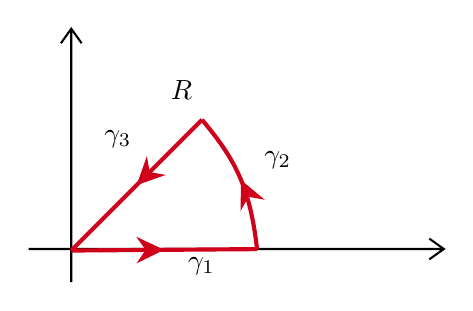
\begin{tikzpicture}[x=0.75pt,y=0.75pt,yscale=-1,xscale=1]
%uncomment if require: \path (0,176); %set diagram left start at 0, and has height of 176

%Shape: Axis 2D [id:dp17170898643653087] 
\draw  (220,126.6) -- (420,126.6)(240.5,20.47) -- (240.5,142.55) (413,121.6) -- (420,126.6) -- (413,131.6) (235.5,27.47) -- (240.5,20.47) -- (245.5,27.47)  ;
%Straight Lines [id:da9725409241349892] 
\draw [color={rgb, 255:red, 208; green, 2; blue, 27 }  ,draw opacity=1 ][line width=1.5]    (240.5,127.34) -- (303.5,64.34) ;
\draw [shift={(272,95.84)}, rotate = 315] [fill={rgb, 255:red, 208; green, 2; blue, 27 }  ,fill opacity=1 ][line width=0.08]  [draw opacity=0] (13.4,-6.43) -- (0,0) -- (13.4,6.44) -- (8.9,0) -- cycle    ;
%Curve Lines [id:da9846937875734199] 
\draw [color={rgb, 255:red, 208; green, 2; blue, 27 }  ,draw opacity=1 ][line width=1.5]    (303.5,64.34) .. controls (318.5,82.34) and (326.5,95.34) .. (330,126.66) ;
\draw [shift={(322.31,93.38)}, rotate = 65.41] [fill={rgb, 255:red, 208; green, 2; blue, 27 }  ,fill opacity=1 ][line width=0.08]  [draw opacity=0] (13.4,-6.43) -- (0,0) -- (13.4,6.44) -- (8.9,0) -- cycle    ;
%Straight Lines [id:da17260088434526732] 
\draw [color={rgb, 255:red, 208; green, 2; blue, 27 }  ,draw opacity=1 ][line width=1.5]    (240.5,127.34) -- (330,126.66) ;
\draw [shift={(285.25,127)}, rotate = 539.56] [fill={rgb, 255:red, 208; green, 2; blue, 27 }  ,fill opacity=1 ][line width=0.08]  [draw opacity=0] (13.4,-6.43) -- (0,0) -- (13.4,6.44) -- (8.9,0) -- cycle    ;

% Text Node
\draw (255,67.95) node [anchor=north west][inner sep=0.75pt]    {$\gamma _{3}$};
% Text Node
\draw (332,77.95) node [anchor=north west][inner sep=0.75pt]    {$\gamma _{2}$};
% Text Node
\draw (295.25,129.4) node [anchor=north west][inner sep=0.75pt]    {$\gamma _{1}$};
% Text Node
\draw (287,43.95) node [anchor=north west][inner sep=0.75pt]    {$R$};


\end{tikzpicture}
\end{figure}
\FloatBarrier

le cui parti sono parametrizzate come segue
\begin{itemize}
\item $\gamma _{1}\left( t\right) =t$ con $t\in \left[ 0,R\right]$
\item $\gamma _{2}\left( t\right) =Re^{it}$ con $t\in \left[ 0,\frac{\pi }{4}\right]$
\item $-\gamma _{3}\left( t\right) =te^{i\frac{\pi }{4}}$ con $t\in \left[ 0,R\right]$
\end{itemize}

Analizziamo cosa succede all'integrale di $f\left( z\right)$ sui vari percorsi
\begin{itemize}
\item su $\gamma _{1}$\begin{equation*}
\int\nolimits _{\gamma _{1}} f\left( z\right) dz=\int\nolimits ^{R}_{0} e^{it^{2}} dt\xrightarrow{R\rightarrow +\infty }\int\nolimits ^{+\infty }_{0} e^{it^{2}} dt=J
\end{equation*}
\item su $\gamma _{3}$\begin{align*}
\int\nolimits _{\gamma _{3}} f\left( z\right) dz & =-\int\nolimits ^{R}_{0} f\left( \gamma \left( t\right)\right) \gamma '\left( t\right) dt=-\int\nolimits ^{R}_{0} e^{it^{2} e^{i\frac{\pi }{2}}} e^{i\frac{\pi }{4}} dt\\
 & =-\int\nolimits ^{R}_{0} e^{it^{2} i} e^{i\frac{\pi }{4}} dt=-e^{i\frac{\pi }{4}}\int\nolimits ^{R}_{0} e^{-t^{2}} dt\xrightarrow{R\rightarrow +\infty } -e^{i\frac{\pi }{4}}\int\nolimits ^{+\infty }_{0} e^{-t^{2}} dt
\end{align*}

\begin{nb}
Ricordiamo l'integrale di Gauss
\begin{equation*}
\int\nolimits _{\mathbb{R}} e^{-x^{2}} dx=\sqrt{\pi }
\end{equation*}
\end{nb}

Otteniamo che\begin{equation*}
\int\nolimits _{\gamma _{3}} f\left( z\right) dz\xrightarrow{R\rightarrow +\infty } -e^{i\frac{\pi }{4}}\frac{\sqrt{\pi }}{2}
\end{equation*}
\item su $\gamma _{2}$ dobbiamo cercare una maggiorazione in modo da far vedere che tende a $0$. Ricordiamo anche che $\left| e^{z}\right| =e^{\mathrm{Re}\left( z\right)}$\begin{align*}
0 & \leqslant \left| \int\nolimits _{\gamma _{2}} f\left( z\right) dz\right| =\left| \int\nolimits ^{\pi /4}_{0} f\left( \gamma \left( t\right)\right) \gamma '\left( t\right) dt\right| =\left| \int\nolimits ^{\pi /4}_{0} e^{iR^{2} e^{2it}} Rie^{it} dt\right| \\
 & \leqslant R\int\nolimits ^{\pi /4}_{0}\left| e^{iR^{2} e^{2it}}\right| dt=R\int\nolimits ^{\pi /4}_{0}\left| e^{iR^{2} e^{2it}}\right| dt=R\int\nolimits ^{\pi /4}_{0} e^{\mathrm{Re}\left[ iR^{2}\left(\cos\left( 2t\right) +i\sin\left( 2t\right)\right)\right]} dt\\
 & =R\int\nolimits ^{\pi /4}_{0} e^{-R^{2}\sin\left( 2t\right)} dt=\left\{\begin{array}{ c }
2t=x\\
dt=\frac{dx}{2}
\end{array}\right\} =\frac{R}{2}\int\nolimits ^{\pi /2}_{0} e^{-R^{2}\sin x} dx
\end{align*}

minoriamo ora il seno



\begin{figure}[htpb]
	\centering
\tikzset{every picture/.style={line width=0.75pt}} %set default line width to 0.75pt        

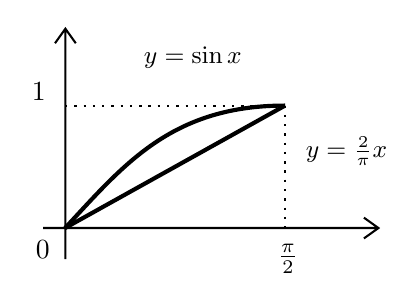
\begin{tikzpicture}[x=0.75pt,y=0.75pt,yscale=-1,xscale=1]
%uncomment if require: \path (0,140); %set diagram left start at 0, and has height of 140

%Shape: Axis 2D [id:dp521862829598075] 
\draw  (200,100.03) -- (361.5,100.03)(210.67,4) -- (210.67,115.03) (354.5,95.03) -- (361.5,100.03) -- (354.5,105.03) (205.67,11) -- (210.67,4) -- (215.67,11)  ;
%Curve Lines [id:da7711478785582004] 
\draw [line width=1.5]    (210.5,100.03) .. controls (238.5,70.03) and (261.5,41.03) .. (316.5,41.03) ;
%Straight Lines [id:da5280090308997825] 
\draw  [dash pattern={on 0.84pt off 2.51pt}]  (210.5,41.03) -- (316.5,41.03) ;
%Straight Lines [id:da665885556586004] 
\draw  [dash pattern={on 0.84pt off 2.51pt}]  (316.5,41.03) -- (316.5,100.03) ;
%Straight Lines [id:da2630936419717216] 
\draw [line width=1.5]    (316.5,41.03) -- (210.5,100.03) ;

% Text Node
\draw (193,28.4) node [anchor=north west][inner sep=0.75pt]    {$1$};
% Text Node
\draw (311.5,106.43) node [anchor=north west][inner sep=0.75pt]    {$\frac{\pi }{2}$};
% Text Node
\draw (195,104.4) node [anchor=north west][inner sep=0.75pt]    {$0$};
% Text Node
\draw (325,54.4) node [anchor=north west][inner sep=0.75pt]  [font=\small]  {$y=\frac{2}{\pi } x$};
% Text Node
\draw (247,11.4) node [anchor=north west][inner sep=0.75pt]  [font=\small]  {$y=\sin x$};


\end{tikzpicture}
\end{figure}
\FloatBarrier


otteniamo\begin{align*}
\frac{R}{2}\int\nolimits ^{\pi /2}_{0} e^{-R^{2}\sin x} dx & \leqslant \frac{R}{2}\int\nolimits ^{\pi /2}_{0} e^{-\frac{2}{\pi } R^{2} x} dx\\
 & =\frac{R}{2}\left[ -\frac{\pi }{2R^{2}} e^{-\frac{2R^{2}}{\pi } x}\right]^{\pi /2}_{0} =\frac{\pi }{4R}\left( 1-e^{-R^{2}}\right)\xrightarrow{R\rightarrow +\infty } 0
\end{align*}
\end{itemize}

Per il teorema dell'integrale nullo di Cauchy
\begin{equation*}
0=\oint\nolimits _{\gamma } f\left( z\right) dz=\int\nolimits _{\gamma _{1}} f\left( z\right) dz+\int\nolimits _{\gamma _{2}} f\left( z\right) dz+\int\nolimits _{\gamma _{3}} f\left( z\right) dz
\end{equation*}
sostituiamo i vari elementi, sempre per $R\rightarrow +\infty $
\begin{equation*}
0=J+0-e^{i\frac{\pi }{4}}\frac{\sqrt{\pi }}{2}
\end{equation*}
allora
\begin{equation*}
J=\int\nolimits ^{+\infty }_{0} e^{it^{2}} dt=e^{i\frac{\pi }{4}}\frac{\sqrt{\pi }}{2} =\frac{\sqrt{2\pi }}{4}\left( 1+i\right)
\end{equation*}
ma quindi
\begin{align*}
\int\nolimits ^{+\infty }_{0}\cos t^{2} dt & =\mathrm{Re}\left( J\right) =\frac{\sqrt{2\pi }}{4}\\
\int\nolimits ^{+\infty }_{0}\sin t^{2} dt & =\mathrm{Im}\left( J\right) =\frac{\sqrt{2\pi }}{4}
\end{align*}
\Soluzione
\begin{align*}
f\left( z\right) = & \sum\limits ^{\infty }_{n=-\infty }\frac{z^{2n}}{9^{\left| n\right| }} =\sum _{n< 0}\frac{z^{2n}}{9^{\left| n\right| }} +\sum _{n\geqslant 0}\frac{z^{2n}}{9^{n}}\\
 & =\sum _{n >0}\frac{z^{-2n}}{9^{n}} +\sum _{n\geqslant 0}\frac{z^{2n}}{9^{n}}\\
 & =\sum _{n >0}\frac{1}{9^{n} z^{2n}} +\sum _{n\geqslant 0}\frac{z^{2n}}{9^{n}}
\end{align*}
Affinché la serie di Laurent converga devono convergere entrambe le serie. La prima converge se
\begin{equation*}
\lim\limits _{n\rightarrow \infty }\left| \frac{a_{n+1}}{a_{n}}\right| =\lim\limits _{n\rightarrow \infty }\frac{9^{n}\left| z\right| ^{2n}}{9^{n+1}\left| z\right| ^{2\left( n+1\right)}} =\frac{1}{9\left| z\right| ^{2}} < 1
\end{equation*}
ossia $\left| z\right| ^{2}  >\frac{1}{9}$, cioè $\left| z\right|  >\frac{1}{3}$.

La seconda serie converge se
\begin{equation*}
\lim\limits _{n\rightarrow \infty }\left| \frac{b_{n+1}}{b_{n}}\right| =\lim\limits _{n\rightarrow \infty }\frac{\left| z\right| ^{2\left( n+1\right)}}{9^{n+1}}\frac{9^{n}}{\left| z\right| ^{2n}} =\frac{1}{9}\left| z\right| ^{2} < 1
\end{equation*}
ossia $\left| z\right| ^{2} < 9$, cioè $\left| z\right| < 3$.

Allora l'anello di convergenza è $A=\left\{z\in \mathbb{C} :\frac{1}{3} < \left| z\right| < 3\right\}$.
\Soluzione

Possiamo vedere la $f$ come
\begin{equation*}
f\left( z\right) =\frac{1}{2iz-z^{2}} =\frac{1}{z\left( 2i-z\right)} =\frac{1}{z} \cdotp \frac{1}{2i} \cdotp \frac{1}{1-\frac{z}{2i}}
\end{equation*}
In $A$
\begin{align*}
f\left( z\right) & =\frac{1}{z} \cdotp \frac{1}{2i} \cdotp \frac{1}{1-\frac{z}{2i}} =\frac{1}{z} \cdotp \frac{1}{2i} \cdotp \sum\limits ^{\infty }_{n=0}\frac{z^{n}}{\left( 2i\right)^{n}}\\
 & =\sum\limits ^{\infty }_{n=0}\frac{z^{n-1}}{\left( 2i\right)^{n+1}} =\sum\limits ^{\infty }_{n=-1}\frac{z^{n}}{\left( 2i\right)^{n+2}}
\end{align*}
In $B$
\begin{align*}
f\left( z\right) & =\frac{1}{z\left( 2i-z\right)} =\frac{A}{z} +\frac{B}{2i-z} =\frac{A2i-Az+Bz}{z\left( 2i-z\right)} =\frac{A2i+z\left( B-A\right)}{z\left( 2i-z\right)}
\end{align*}
allora $A=B=-\frac{i}{2}$
\begin{align*}
f\left( z\right) & =-\frac{i}{2}\left\{\frac{1}{z} +\frac{1}{2i-z}\right\}\\
 & =-\frac{i}{2}\left\{\frac{1}{\left( z-2i\right) +2i} +\frac{1}{2i-z}\right\}\\
 & =-\frac{i}{2}\left\{\frac{1}{z-2i} \cdotp \frac{1}{1+\frac{2i}{z-2i}} +\frac{1}{2i-z}\right\}\\
 & =-\frac{i}{2}\left\{\frac{1}{z-2i} \cdotp \frac{1}{1-\frac{-2i}{z-2i}} -\frac{1}{z-2i}\right\}
\end{align*}
Essendo in $B$
\begin{equation*}
\left| \frac{-2i}{z-2i}\right| < 1\ \ \Leftrightarrow \ \ 2< \left| z-2i\right| 
\end{equation*}
possiamo scrivere la serie geometrica
\begin{align*}
f\left( z\right) & =-\frac{i}{2}\left\{\frac{1}{z-2i} \cdotp \sum\limits ^{\infty }_{n=0}\left(\frac{-2i}{z-2i}\right)^{n} -\frac{1}{z-2i}\right\}\\
 & =-\frac{i}{2}\left\{\frac{1}{z-2i}\left[\sum\limits ^{\infty }_{n=0}\left(\frac{-2i}{z-2i}\right)^{n} -1\right]\right\}\\
 & =-\frac{i}{2}\left\{\frac{1}{z-2i}\sum\limits ^{\infty }_{n=1}\left(\frac{-2i}{z-2i}\right)^{n}\right\}\\
 & =-\frac{i}{2}\left\{\sum\limits ^{\infty }_{n=1}\frac{\left( -2i\right)^{n}}{\left( z-2i\right)^{n+1}}\right\}
\end{align*}
\Soluzione
\begin{theorem}
Sia $f\in \mathcal{H}\left( D\left( z_{0} ,R\right) \setminus \left\{z_{0}\right\}\right)$, cioè $z_{0}$ è una \textbf{singolarità isolata} per $f$. Allora localmente
\begin{equation*}
f\left( z\right) =\sum\limits ^{+\infty }_{n=-\infty } a_{n}\left( z-z_{0}\right)^{n}
\end{equation*}
\end{theorem}
\begin{theorem}
Sia $M=\left\{n\in \mathbb{Z} :n< 0,a_{n} \neq 0\right\}$ l'insieme degli indici della parte singolare dello sviluppo di Laurent. $z_{0}$ è

\begin{itemize}
\item \textbf{singolarità eliminabile} se

\begin{equation*}
\exists \lim\limits _{z\rightarrow z_{0}} f\left( z\right) \in \mathbb{C} \ \ \Leftrightarrow \ \ M=\emptyset \ \ \Leftrightarrow \ \ f\ \text{è limitata su} \ \mathcal{U}\left( z_{0}\right)
\end{equation*}
\item \textbf{polo} se

\begin{equation*}
\exists \lim\limits _{z\rightarrow z_{0}} f\left( z\right) =\infty \ \ \Leftrightarrow \ \ 0< \left| M\right| < +\infty 
\end{equation*}

dove $-\min M=k$ è l'\textbf{ordine} del polo.
\item \textbf{singolarità essenziale} se

\begin{gather*}
\nexists \lim\limits _{z\rightarrow z_{0}} f\left( z\right) \ \ \Leftrightarrow \ \ \left| M\right| =\infty \\
\Leftrightarrow \ \ \forall \varepsilon \in \left( 0,R\right) \ \text{l'insieme immagine} \ f\left(\left\{0< \left| z-z_{0}\right| < \varepsilon \right\}\right) \ \text{è denso in} \ \mathbb{C}
\end{gather*}
\end{itemize}
\end{theorem}
\begin{definition}
Si dice residuo di $f$ in $z_{0}$
\begin{equation*}
\mathrm{Res}\left( f,z_{0}\right) :=a_{-1}
\end{equation*}
\end{definition}
\begin{theorem}
Sia $f\in \mathcal{H}\left(\mathbb{C} \setminus \overline{D\left( z_{0} ,R\right)}\right)$ ed $M=\left\{n\in \mathbb{Z} :n >0,a_{n} \neq 0\right\}$. Il punto $\infty $ è

\begin{itemize}
\item \textbf{singolarità eliminabile} se e solo se\begin{equation*}
\exists \lim\limits _{z\rightarrow \infty } f\left( z\right) \in \mathbb{C} \ \ \Leftrightarrow \ \ M=\emptyset 
\end{equation*}
\item \textbf{polo} se e solo se\begin{equation*}
\exists \lim\limits _{z\rightarrow \infty } f\left( z\right) =\infty \ \ \Leftrightarrow \ \ 0< \left| M\right| < \infty 
\end{equation*}
\item \textbf{singolarità essenziale} se e solo se\begin{equation*}
\nexists \lim\limits _{z\rightarrow +\infty } f\left( z\right) \ \ \Leftrightarrow \ \ \left| M\right| =\infty 
\end{equation*}
\end{itemize}
\end{theorem}
\begin{definition}
Si dice residuo di $f$ in $\infty $
\begin{equation*}
\mathrm{Res}\left( f,\infty \right) :=-a_{-1}
\end{equation*}
\end{definition}
\begin{theorem}
[di De l'Hôpital] Siano $f$ e $g$ funzioni analitiche in $B_{R}\left( z_{0}\right)$ tali che $f\left( z_{0}\right) =g\left( z_{0}\right) =0$ e $g'\left( z_{0}\right) \neq 0$ (quindi solo la forma $\frac{0}{0}$ al finito). Allora
\begin{equation*}
\lim\limits _{z\rightarrow z_{0}}\frac{f\left( z\right)}{g\left( z\right)} =\frac{f'\left( z_{0}\right)}{g'\left( z_{0}\right)}
\end{equation*}
\end{theorem}
\begin{theorem}
Le seguenti affermazioni sono equivalenti
\begin{itemize}
\item $f$ ha in $z_{0}$ un polo di ordine $m$
\item $g\left( z\right) =\left( z-z_{0}\right)^{m} f\left( z\right)$ ha in $z_{0}$ una singolarità eliminabile e $\lim\limits _{z\rightarrow z_{0}} g\left( z\right) \neq 0$
\item $f\left( z\right) \approx \left| z-z_{0}\right| ^{m}$ per $z\rightarrow z_{0}$
\item $\frac{1}{f\left( z\right)}$ ha in $z_{0}$ uno zero di ordine $m$
\end{itemize}
\end{theorem}
\begin{theorem}
Siano $f(z)$ e $g(z)$ tali che $f\left( z_{0}\right) =0=g\left( z_{0}\right)$ e siano $n$ ed $m$ rispettivamente, gli ordini di $z_{0}$ come zero di $f$ e $g$. La funzione $\frac{f(z)}{g(z)}$ ha in $z_{0}$:

\begin{itemize}
\item una singolarità eliminabile che è uno zero d'ordine $n-m$ se e solo se $n >m$
\item una singolarità eliminabile che non è uno zero se e solo se $n=m$
\item un polo d'ordine $m-n$ se e solo se $m >n$.
\end{itemize}
\end{theorem}
\begin{theorem}
Sia $f\in \mathcal{H}\left(\mathbb{C} \setminus \left\{z_{1} ,\dotsc ,z_{n}\right\}\right)$ allora
\begin{equation*}
\sum\limits ^{n}_{k=1}\mathrm{Res}\left( f,z_{k}\right) +\mathrm{Res}\left( f,\infty \right) =0
\end{equation*}
\end{theorem}
\begin{theorem}
Sia $f\in \mathcal{H}\left(\mathbb{C} \setminus \left\{z_{1} ,\dotsc ,z_{n}\right\}\right)$. Se $R >\max_{1\leqslant k\leqslant n}\left| z_{k}\right| $ allora
\begin{equation*}
\int\nolimits _{\partial D\left( 0,R\right)} f\left( z\right) dz=2\pi i\left[\sum\limits ^{n}_{k=1}\mathrm{Res}\left( f,z_{k}\right)\right]
\end{equation*}
\end{theorem}
\begin{nb}
Come si calcolano i residui?
Nei punti all'infinito si definisce
\begin{equation*}
\mathrm{Res}\left( f,\infty \right) =\mathrm{Res}\left( -\frac{1}{z^{2}} f\left(\frac{1}{z}\right) ,0\right)
\end{equation*}
Nei punti $z_{0} \neq \infty $
\begin{enumerate}
\item se è una singolarità eliminabile:\begin{equation*}
\mathrm{Res}\left( f,z_{0}\right) =0
\end{equation*}

(attenzione: solo per i punti finiti)
\item se è un polo, c'è la \textbf{formula dei poli}
\begin{enumerate}
\item semplice (di ordine $p=1$)\begin{equation*}
\mathrm{Res}\left( f,z_{0}\right) =\lim\limits _{z\rightarrow z_{0}} f\left( z\right)\left( z-z_{0}\right)
\end{equation*}
\item di ordine $p\geqslant 2$\begin{equation*}
\mathrm{Res}\left( f,z_{0}\right) =\frac{1}{\left( p-1\right) !}\lim\limits _{z\rightarrow z_{0}}\left\{\frac{d^{p-1}}{dz^{p-1}}\left[ f\left( z\right)\left( z-z_{0}\right)^{p}\right]\right\}
\end{equation*}
\end{enumerate}
\item se è una singolarità essenziale bisogna per forza fare lo sviluppo di Laurent (che è valido in tutti i casi in realtà, ma è decisamente più laborioso la maggior parte delle volte)
\end{enumerate}
\end{nb}
\begin{theorem}
Sia $F=\frac{f}{g}$. Se $f\in \mathcal{H}\left(\mathcal{U}\left( z_{0}\right)\right)$ e $g$ ha in $z_{0}$ uno zero semplice ($g\left( z_{0}\right) =0$ e $g'\left( z_{0}\right) \neq 0$), allora\begin{equation*}
\mathrm{Res}\left(\frac{f}{g} ,z_{0}\right) =\frac{f\left( z_{0}\right)}{g'\left( z_{0}\right)}
\end{equation*}

Ricordiamo che se $f$ non si annulla in $z_{0}$ allora $F$ ha in $z_{0}$ un polo del I ordine. Se $f$ si annulla in $z_{0}$ allora $F$ ha in $z_{0}$ una singolarità eliminabile.
\end{theorem}
Le singolarità isolate sono $0,1,-1,\infty $.

$z=0,z=1,z=-1$ annullano il denominatore con molteplicità $1$ e non annullano il numeratore, quindi sono degli $1$-poli. Per il teorema appena enunciato:
\begin{align*}
\mathrm{Res}\left( F,\phantom{-}0\right) &=\left\{g\left( z\right) =  z,\ f\left( z\right) =\frac{1}{1-z^{2}}\right\} =\frac{1}{1} =1\\
\mathrm{Res}\left( F,\phantom{-}1\right) &=\left\{g\left( z\right) =1-z,\ f\left( z\right) =\frac{1}{z\left( 1+z\right)}\right\} =\frac{\frac{1}{2}}{-1} =-\frac{1}{2}\\
\mathrm{Res}\left( F,-1\right) 			 &=\left\{g\left( z\right) =1+z,\ f\left( z\right) =\frac{1}{z\left( 1-z\right)}\right\} =-\frac{1}{2}
\end{align*}
Mentre
\begin{equation*}
F\left( z\right) =\frac{1}{z\left( 1+z\right)\left( 1-z\right)} \sim \frac{1}{z^{3}} \ \ \ \ z\rightarrow +\infty 
\end{equation*}
quindi $\infty $ è una singolarità eliminabile.
\begin{equation*}
\mathrm{Res}\left( F,\infty \right) =-\sum\limits ^{3}_{k=1}\mathrm{Res}\left( F,z_{k}\right) =-\left( 1-\frac{1}{2} -\frac{1}{2}\right) =0
\end{equation*}
\begin{obs}
Se $\infty $ è singolarità eliminabile, ciò non implica per forza $\mathrm{Res}\left( f,\infty \right) =0$. Infatti $f\left( z\right) =\frac{1}{z}\rightarrow 0$ per $z\rightarrow +\infty $ quindi $\infty $ è singolarità eliminabile, ma $\mathrm{Res}\left( f,\infty \right) =-a_{-1} =-1\neq 0$.
\end{obs}
\begin{nb}
Nel nostro caso è vero perchè vale il seguente teorema.
\end{nb}
\begin{theorem}
Se $f$ ha uno zero di ordine almeno $2$ in $\infty $ allora $\mathrm{Res}\left( f,\infty \right) =0$, perché
\begin{equation*}
f\left( z\right) =\sum\limits ^{-2}_{n=-\infty } a_{n} z^{n} \ \ \Rightarrow \ \ \mathrm{Res}\left( f,\infty \right) =-a_{-1} =0
\end{equation*}
\end{theorem}
\Soluzione

Le singolarità isolate di $f$ sono $i,\infty $.

$z=i$ annulla il denominatore con molteplicità $2$ e non annulla il numeratore, quindi è un polo. Usando la formula dei poli
\begin{equation*}
\mathrm{Res}\left( f,i\right) =\frac{d}{dz} f\left( z\right)\left( z-i\right)^{2} =\left. -5z^{4}\right| _{z=i} =-5
\end{equation*}
$f\left( z\right) \sim -z^{3}$ per $z\rightarrow +\infty $ quindi $\infty $ è un $3$-polo.
\begin{equation*}
\mathrm{Res}\left( f,\infty \right) =-\mathrm{Res}\left( f,i\right) =5
\end{equation*}
\Soluzione

Le singolarità isolate di $f$ sono $1,0,\pm 2i,\infty $.

$z=\pm 2i$ sono zeri di molteplicità $1$ per il denominatore di $f$ e non annullano il denominatore, quindi sono $1$-poli. Usando la formula dei poli
\begin{gather*}
\mathrm{Res}\left( f,2i\right) =\lim\limits _{z\rightarrow 2i}\left( z-2i\right) f\left( z\right) =\dotsc =\frac{e^{-\frac{1+2i}{5}}}{16} i\\
\mathrm{Res}\left( f,-2i\right) =\lim\limits _{z\rightarrow -2i}\left( z+2i\right) f\left( z\right) =\dotsc =-\frac{e^{\frac{2i-1}{5}}}{16} i
\end{gather*}
$z=0$ è uno zero di molteplicità $2$ per il denominatore di $f$ e non annulla il denominatore, quindi è un $2$-polo. Usando la formula dei poli
\begin{equation*}
\mathrm{Res}\left( f,0\right) =\lim\limits _{z\rightarrow 0}\frac{d}{dz} z^{2} f\left( z\right) =\dotsc =-\frac{1}{4e}
\end{equation*}
$z=1$ è una singolarità essenziale perché $\nexists \lim\limits _{z\rightarrow 1} f\left( z\right)$.

Abbiamo che $f\left( z\right) \sim \frac{e}{z^{4}}$ per $z\rightarrow +\infty $, allora per il teorema $\mathrm{Res}\left( f,\infty \right) =0$.

Infine
\begin{equation*}
\mathrm{Res}\left( f,1\right) =-\sum \mathrm{Res}\left( f,\dotsc \right) =\frac{1}{4e} -\frac{\sin\left(\frac{2}{5}\right)}{8e^{\frac{1}{5}}}
\end{equation*}
\Soluzione
\begin{enumerate}
\item Le singolarità di $f$ sono $1,2,\infty $.

$z=1$ è singolarità essenziale perché $\nexists \lim\limits _{z\rightarrow 1} f\left( z\right)$

$z=2$ è $1$-polo perché annulla il denominatore con molteplicità $1$ e non annulla il numeratore.

$z=\infty $ è singolarità eliminabile perché $\exists \lim\limits _{z\rightarrow \infty } f\left( z\right) \in \mathbb{C}$.
\item Ricordiamo che

\begin{nb}
\begin{equation*}
e^{z} =\sum\limits ^{\infty }_{n=0}\frac{z^{n}}{n!} ,\ \ z\in \mathbb{C} \ \ \ \ \ \ \ \ \frac{1}{1-z} =\sum\limits ^{\infty }_{n=0} z^{n} ,\ \ \left| z\right| < 1
\end{equation*}
\end{nb}

Qui\begin{equation*}
e^{\frac{1}{z-1}} =\sum\limits ^{\infty }_{h=0}\frac{1}{h!\left( z-1\right)^{h}}
\end{equation*}mentre\begin{equation*}
\frac{1}{z-2} =-\frac{1}{2-z} =-\frac{1}{1-\left( z-1\right)} =-\sum\limits ^{\infty }_{k=0}\left( z-1\right)^{k}
\end{equation*}La prima serie converge in $\left| z-1\right|  >0$ e la seconda in $\left| z-1\right| < 1$. La serie di Laurent converge quindi in $0< \left| z-1\right| < 1$.\begin{nb}
Per scrivere la serie di Laurent sfruttiamo il prodotto alla Cauchy.
\begin{equation*}
\left(\sum\limits ^{\infty }_{n=0} a_{n}\right)\left(\sum\limits ^{\infty }_{n=0} b_{n}\right) =\sum\limits ^{\infty }_{n=0}\left(\sum\limits ^{n}_{k=0} a_{k} b_{n-k}\right)
\end{equation*}
\end{nb}Quindi\begin{equation*}
f\left( z\right) =-\sum\limits ^{\infty }_{k=0}\sum\limits ^{k}_{h=0}\frac{\left( z-1\right)^{k-2h}}{h!}
\end{equation*}
\item $\mathrm{Res}\left( f,2\right) =e$ per la formula dei poli

$\mathrm{Res}\left( f,1\right) =a_{-1}$ lo trovo ponendo $k-2h=-1$, quindi $a_{-1} =-\sum\limits ^{\infty }_{h=1}\frac{1}{h!} =1-e$

$\mathrm{Res}\left( f,\infty \right) =-1$
\item Applico il teorema dei residui\begin{equation*}
\int\nolimits _{\gamma } f\left( z\right) dz=2\pi i\left[\mathrm{Res}\left( f,1\right) +\mathrm{Res}\left( f,2\right)\right] =2\pi i
\end{equation*}
\end{enumerate}
\chapter{Esercitazione 3 - Boella}
\ParteEsercizi
\Esercizio{}

Calcolare il seguente integrale
\begin{equation*}
\int _{\mathbb{R}}\frac{1}{x^{4} +4a^{4}} dx
\end{equation*}
\Esercizio{}

Calcolare il seguente integrale
\begin{equation*}
\int _{\mathbb{R}}\frac{e^{-i\lambda x}}{x^{6} +64} dx\ \ \ \ \forall \lambda \in \mathbb{R}
\end{equation*}
\Esercizio{}

Calcolare il seguente integrale
\begin{equation*}
\int ^{\pi }_{0}\frac{1}{a+b\cos \vartheta } d\vartheta \ \ \ \ 0< b< a
\end{equation*}
\Esercizio{}

Calcolare il seguente integrale, per i valori di $\alpha $ in cui converge
\begin{equation*}
\int _{\mathbb{R}}\frac{e^{\alpha x}}{1+e^{x}} dx\ \ \ \ \alpha \in \mathbb{R}
\end{equation*}
\Esercizio{}

Calcolare il seguente integrale
\begin{equation*}
\int ^{+\infty }_{0}\frac{\cos\left( \alpha x\right)}{x^{2} +\beta ^{2}} dx\ \ \ \ \alpha \neq 0,\beta \neq 0
\end{equation*}
\ParteSoluzioni
\Soluzione

Per cominciare pensiamo il nostro integrale come
\begin{equation*}
\int _{\mathbb{R}}\frac{1}{x^{4} +4a^{4}} dx=\lim\limits _{R\rightarrow +\infty }\int ^{R}_{-R}\frac{1}{x^{4} +4a^{4}} dx
\end{equation*}
Consideriamo un percorso $\gamma _{R}$ fatto dall'unione della curva da $-R$ a $R$ e la semicirconferenza di raggio $R$ che chiameremo $\sigma _{R}$


\begin{figure}[htpb]
	\centering
\tikzset{every picture/.style={line width=0.75pt}} %set default line width to 0.75pt        

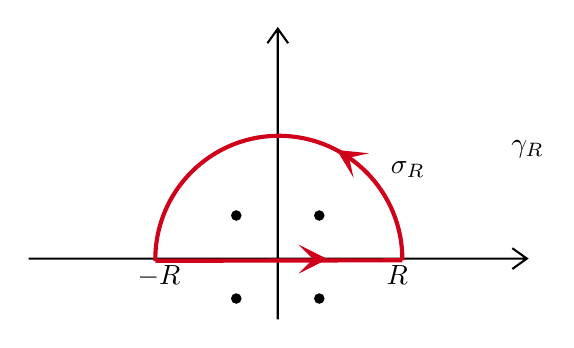
\begin{tikzpicture}[x=0.75pt,y=0.75pt,yscale=-1,xscale=1]
%uncomment if require: \path (0,179); %set diagram left start at 0, and has height of 179

%Shape: Axis 2D [id:dp39099083924259226] 
\draw  (180,120.75) -- (420,120.75)(300,10) -- (300,150) (413,115.75) -- (420,120.75) -- (413,125.75) (295,17) -- (300,10) -- (305,17)  ;
%Shape: Arc [id:dp3884788829218313] 
\draw  [draw opacity=0][line width=1.5]  (241,121.83) .. controls (241,121.59) and (241,121.34) .. (241,121.09) .. controls (241,88.23) and (267.64,61.59) .. (300.5,61.59) .. controls (333.36,61.59) and (360,88.23) .. (360,121.09) .. controls (360,121.25) and (360,121.41) .. (360,121.57) -- (300.5,121.09) -- cycle ; \draw  [color={rgb, 255:red, 208; green, 2; blue, 27 }  ,draw opacity=1 ][line width=1.5]  (241,121.83) .. controls (241,121.59) and (241,121.34) .. (241,121.09) .. controls (241,88.23) and (267.64,61.59) .. (300.5,61.59) .. controls (333.36,61.59) and (360,88.23) .. (360,121.09) .. controls (360,121.25) and (360,121.41) .. (360,121.57) ;
%Shape: Circle [id:dp8434618645208203] 
\draw  [fill={rgb, 255:red, 0; green, 0; blue, 0 }  ,fill opacity=1 ] (278,100) .. controls (278,98.9) and (278.9,98) .. (280,98) .. controls (281.1,98) and (282,98.9) .. (282,100) .. controls (282,101.1) and (281.1,102) .. (280,102) .. controls (278.9,102) and (278,101.1) .. (278,100) -- cycle ;
%Shape: Circle [id:dp7789399295573649] 
\draw  [fill={rgb, 255:red, 0; green, 0; blue, 0 }  ,fill opacity=1 ] (278,140) .. controls (278,138.9) and (278.9,138) .. (280,138) .. controls (281.1,138) and (282,138.9) .. (282,140) .. controls (282,141.1) and (281.1,142) .. (280,142) .. controls (278.9,142) and (278,141.1) .. (278,140) -- cycle ;
%Shape: Circle [id:dp730262806413829] 
\draw  [fill={rgb, 255:red, 0; green, 0; blue, 0 }  ,fill opacity=1 ] (318,100) .. controls (318,98.9) and (318.9,98) .. (320,98) .. controls (321.1,98) and (322,98.9) .. (322,100) .. controls (322,101.1) and (321.1,102) .. (320,102) .. controls (318.9,102) and (318,101.1) .. (318,100) -- cycle ;
%Shape: Circle [id:dp7565318380097881] 
\draw  [fill={rgb, 255:red, 0; green, 0; blue, 0 }  ,fill opacity=1 ] (318,140) .. controls (318,138.9) and (318.9,138) .. (320,138) .. controls (321.1,138) and (322,138.9) .. (322,140) .. controls (322,141.1) and (321.1,142) .. (320,142) .. controls (318.9,142) and (318,141.1) .. (318,140) -- cycle ;
\draw  [draw opacity=0][fill={rgb, 255:red, 208; green, 2; blue, 27 }  ,fill opacity=1 ] (310,114) -- (324,121) -- (310,128) -- (317,121) -- cycle ;
%Straight Lines [id:da6746169366745891] 
\draw [color={rgb, 255:red, 208; green, 2; blue, 27 }  ,draw opacity=1 ][line width=1.5]    (241,121.83) -- (360,121.57) ;
\draw  [draw opacity=0][fill={rgb, 255:red, 208; green, 2; blue, 27 }  ,fill opacity=1 ] (336.51,81.83) -- (328.43,68.42) -- (344,70) -- (334.34,72.17) -- cycle ;

% Text Node
\draw (411,62.4) node [anchor=north west][inner sep=0.75pt]    {$\gamma _{R}$};
% Text Node
\draw (353,72.4) node [anchor=north west][inner sep=0.75pt]    {$\sigma _{R}$};
% Text Node
\draw (351,122.4) node [anchor=north west][inner sep=0.75pt]    {$R$};
% Text Node
\draw (231,122.4) node [anchor=north west][inner sep=0.75pt]    {$-R$};


\end{tikzpicture}
\end{figure}
\FloatBarrier

Cerchiamo le singolarità della funzione in campo complesso
\begin{equation*}
z^{4} +4a^{4} =0\ \ \Leftrightarrow \ \ z=\pm a\pm ia
\end{equation*}
Calcoliamo ora l'integrale
\begin{equation*}
\int _{\gamma _{R}} f\left( z\right) dz=\int ^{R}_{-R} f\left( x\right) dx+\int _{\sigma _{R}} f\left( z\right) dz
\end{equation*}
che vale, per il teorema dei residui
\begin{equation*}
\int _{\gamma _{R}} f\left( z\right) dz=2\pi i\left[\mathrm{Res}\left( f,-a+ia\right) +\mathrm{Res}\left( f,a+ia\right)\right]
\end{equation*}
Calcoliamo ora questi residui
\begin{gather*}
\mathrm{Res}\left( f,-a+ia\right) =\frac{g\left( z_{0}\right)}{h'\left( z_{0}\right)} =\left. \frac{1}{4z^{3}}\right| _{z=-a+ia} =\left. \frac{z}{4z^{4}}\right| _{z=-a+ia} =\frac{a+ia}{-16a^{4}}\\
\mathrm{Res}\left( f,a+ia\right) =\frac{g\left( z_{0}\right)}{h'\left( z_{0}\right)} =\left. \frac{1}{4z^{3}}\right| _{z=a+ia} =\left. \frac{z}{4z^{4}}\right| _{z=a+ia} =\frac{-a+ia}{-16a^{4}}
\end{gather*}
Allora
\begin{equation*}
\int _{\gamma _{R}} f\left( z\right) dz=2\pi i\left[\frac{a+ia}{-16a^{4}} +\frac{-a+ia}{-16a^{4}}\right] =\frac{\pi }{4a^{3}}
\end{equation*}
Ci resta da far vedere che
\begin{equation*}
\int _{\sigma _{R}} f\left( z\right) dz\rightarrow 0
\end{equation*}
Non possiamo usare il Lemma di Jordan, perché al numeratore non c'è un esponenziale immaginario. Dobbiamo sporcarci le mani. In generale sarà un numero complesso, quindi conviene prenderne il modulo e maggiorarlo.
\begin{nb}
\begin{equation*}
\left| \int _{\gamma } f\left( z\right) dz\right| \leqslant M\cdotp \text{lunghezza}\left( \gamma \right)
\end{equation*}
dove $M$ è il massimo valore che $f$ può assumere lungo $\gamma $.
\end{nb}
Per la disuguaglianza triangolare
\begin{equation*}
\left| a\pm b\right| \geqslant \left| a\right| -\left| b\right| 
\end{equation*}
nel nostro caso
\begin{equation*}
\left| \frac{1}{z^{4} +4a^{4}}\right| =\frac{1}{\left| z^{4} +4a^{4}\right| } \leqslant \frac{1}{\left| z^{4}\right| -\left| 4a^{4}\right| } =\frac{1}{R^{4} -\left| 4a^{4}\right| }
\end{equation*}
e quindi utilizzando il Nota Bene
\begin{equation*}
\left| \int _{\sigma _{R}} f\left( z\right) dz\right| \leqslant \frac{1}{R^{4} -\left| 4a^{4}\right| } \cdotp \pi R\xrightarrow{R\rightarrow \infty } 0
\end{equation*}
Pertanto il nostro integrale iniziale vale
\begin{equation*}
\int _{\mathbb{R}}\frac{1}{x^{4} +4a^{4}} dx=\frac{\pi }{4a^{3}}
\end{equation*}
\Soluzione
\begin{theorem}
Lemmi di Jordan. Considerando
\begin{equation*}
g\left( z\right) e^{i\alpha z}
\end{equation*}
\begin{itemize}
\item $\alpha  >0$ l'integrale sulla semicirconferenza di sopra tende a zero
\item $\alpha < 0$ l'integrale sulla semicirconferenza di sotto tende a zero (quello sopra fa un casino dell'altro mondo)
\end{itemize}
\end{theorem}
Analizziamo il caso $\lambda  >0$. Applichiamo il Lemma di Jordan, il quale ci dice che l'integrale lungo la semicirconferenza inferiore tende a $0$, quindi possiamo direttamente scrivere


\begin{figure}[htpb]
	\centering
\tikzset{every picture/.style={line width=0.75pt}} %set default line width to 0.75pt        

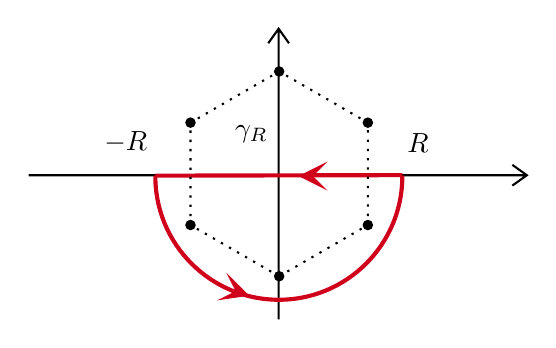
\begin{tikzpicture}[x=0.75pt,y=0.75pt,yscale=-1,xscale=1]
%uncomment if require: \path (0,160); %set diagram left start at 0, and has height of 160

%Shape: Axis 2D [id:dp508857242987794] 
\draw  (170,80) -- (410,80)(290.4,9.41) -- (290.4,149.41) (403,75) -- (410,80) -- (403,85) (285.4,16.41) -- (290.4,9.41) -- (295.4,16.41)  ;
%Shape: Arc [id:dp2429361463821933] 
\draw  [draw opacity=0][line width=1.5]  (350,80.14) .. controls (350,80.26) and (350,80.38) .. (350,80.5) .. controls (350,113.36) and (323.36,140) .. (290.5,140) .. controls (257.64,140) and (231,113.36) .. (231,80.5) .. controls (231,80.4) and (231,80.31) .. (231,80.21) -- (290.5,80.5) -- cycle ; \draw  [color={rgb, 255:red, 208; green, 2; blue, 27 }  ,draw opacity=1 ][line width=1.5]  (350,80.14) .. controls (350,80.26) and (350,80.38) .. (350,80.5) .. controls (350,113.36) and (323.36,140) .. (290.5,140) .. controls (257.64,140) and (231,113.36) .. (231,80.5) .. controls (231,80.4) and (231,80.31) .. (231,80.21) ;
%Shape: Circle [id:dp8781397774455211] 
\draw  [fill={rgb, 255:red, 0; green, 0; blue, 0 }  ,fill opacity=1 ] (288.67,30) .. controls (288.67,28.9) and (289.56,28) .. (290.67,28) .. controls (291.77,28) and (292.67,28.9) .. (292.67,30) .. controls (292.67,31.1) and (291.77,32) .. (290.67,32) .. controls (289.56,32) and (288.67,31.1) .. (288.67,30) -- cycle ;
%Shape: Circle [id:dp3148978419514976] 
\draw  [fill={rgb, 255:red, 0; green, 0; blue, 0 }  ,fill opacity=1 ] (331.39,54.67) .. controls (331.39,53.56) and (332.29,52.67) .. (333.39,52.67) .. controls (334.5,52.67) and (335.39,53.56) .. (335.39,54.67) .. controls (335.39,55.77) and (334.5,56.67) .. (333.39,56.67) .. controls (332.29,56.67) and (331.39,55.77) .. (331.39,54.67) -- cycle ;
%Shape: Circle [id:dp8279624449312546] 
\draw  [fill={rgb, 255:red, 0; green, 0; blue, 0 }  ,fill opacity=1 ] (245.94,104) .. controls (245.94,102.9) and (246.84,102) .. (247.94,102) .. controls (249.05,102) and (249.94,102.9) .. (249.94,104) .. controls (249.94,105.1) and (249.05,106) .. (247.94,106) .. controls (246.84,106) and (245.94,105.1) .. (245.94,104) -- cycle ;
%Shape: Circle [id:dp5338705832900976] 
\draw  [fill={rgb, 255:red, 0; green, 0; blue, 0 }  ,fill opacity=1 ] (331.39,104) .. controls (331.39,102.9) and (332.29,102) .. (333.39,102) .. controls (334.5,102) and (335.39,102.9) .. (335.39,104) .. controls (335.39,105.1) and (334.5,106) .. (333.39,106) .. controls (332.29,106) and (331.39,105.1) .. (331.39,104) -- cycle ;
\draw  [draw opacity=0][fill={rgb, 255:red, 208; green, 2; blue, 27 }  ,fill opacity=1 ] (314,87.41) -- (300,80.41) -- (314,73.41) -- (307,80.41) -- cycle ;
%Straight Lines [id:da4843584145229285] 
\draw [color={rgb, 255:red, 208; green, 2; blue, 27 }  ,draw opacity=1 ][line width=1.5]    (231,80.21) -- (349.99,79.95) ;
\draw  [draw opacity=0][fill={rgb, 255:red, 208; green, 2; blue, 27 }  ,fill opacity=1 ] (265.21,126.99) -- (276.31,138.03) -- (260.82,140.28) -- (269.66,135.83) -- cycle ;
%Shape: Regular Polygon [id:dp2801234129072723] 
\draw  [dash pattern={on 0.84pt off 2.51pt}] (290.67,128.67) -- (247.94,104) -- (247.94,54.67) -- (290.67,30) -- (333.39,54.67) -- (333.39,104) -- cycle ;
%Shape: Circle [id:dp21637549294959646] 
\draw  [fill={rgb, 255:red, 0; green, 0; blue, 0 }  ,fill opacity=1 ] (288.67,128.67) .. controls (288.67,127.56) and (289.56,126.67) .. (290.67,126.67) .. controls (291.77,126.67) and (292.67,127.56) .. (292.67,128.67) .. controls (292.67,129.77) and (291.77,130.67) .. (290.67,130.67) .. controls (289.56,130.67) and (288.67,129.77) .. (288.67,128.67) -- cycle ;
%Shape: Circle [id:dp24691945495063838] 
\draw  [fill={rgb, 255:red, 0; green, 0; blue, 0 }  ,fill opacity=1 ] (245.94,54.67) .. controls (245.94,53.56) and (246.84,52.67) .. (247.94,52.67) .. controls (249.05,52.67) and (249.94,53.56) .. (249.94,54.67) .. controls (249.94,55.77) and (249.05,56.67) .. (247.94,56.67) .. controls (246.84,56.67) and (245.94,55.77) .. (245.94,54.67) -- cycle ;

% Text Node
\draw (268,54.4) node [anchor=north west][inner sep=0.75pt]    {$\gamma _{R}$};
% Text Node
\draw (351,58.4) node [anchor=north west][inner sep=0.75pt]    {$R$};
% Text Node
\draw (205,57.4) node [anchor=north west][inner sep=0.75pt]    {$-R$};


\end{tikzpicture}
\end{figure}
\FloatBarrier

\begin{equation*}
\int _{\mathbb{R}}\frac{e^{-i\lambda x}}{x^{6} +64} dx=-\lim\limits _{R\rightarrow \infty }\int _{\gamma _{R}}\frac{e^{-i\lambda z}}{z^{6} +64} dz=-2\pi i\left[\sum \mathrm{Res}\left( f,z_{k}\right)\right]
\end{equation*}
Gli zeri al denominatore di $f$ sono nelle $6$ radici seste di $-64$ (i vertici di un esagono)
\begin{equation*}
\pm \sqrt{3} \pm i\ \ \ \ \pm 2i
\end{equation*}
Quelli che stanno dentro la parte di piano interessata sono
\begin{equation*}
\pm \sqrt{3} -i\ \ \ \ -2i
\end{equation*}
Per calcolare il residuo in tali punti utilizziamo la formula di calcolo vista anche nel precedente esercizio
\begin{equation*}
\mathrm{Res}\left( f,z_{k}\right) =\left. \frac{e^{-i\lambda z}}{6z^{5}}\right| _{z=z_{k}} =\left. \frac{ze^{-i\lambda z}}{6z^{6}}\right| _{z=z_{k}}
\end{equation*}
Pertanto
\begin{itemize}
\item $\mathrm{Res}\left( f,-\sqrt{3} -i\right) =\frac{\left( -\sqrt{3} -i\right) e^{-i\lambda \left( -\sqrt{3} -i\right)}}{6\cdotp \left( -64\right)}$
\item $\mathrm{Res}\left( f,\sqrt{3} -i\right) =\frac{\left(\sqrt{3} -i\right) e^{-i\lambda \left(\sqrt{3} -i\right)}}{6\cdotp \left( -64\right)}$
\item $\mathrm{Res}\left( f,-2i\right) =\frac{\left( -2i\right) e^{-i\lambda \left( -2i\right)}}{6\cdotp \left( -64\right)}$
\end{itemize}

Allora
\begin{align*}
\int _{\mathbb{R}}\frac{e^{-i\lambda x}}{x^{6} +64} dx & =-2\pi i\left[\frac{\left( -\sqrt{3} -i\right) e^{-i\lambda \left( -\sqrt{3} -i\right)}}{6\cdotp \left( -64\right)} +\frac{\left(\sqrt{3} -i\right) e^{-i\lambda \left(\sqrt{3} -i\right)}}{6\cdotp \left( -64\right)} +\frac{\left( -2i\right) e^{-i\lambda \left( -2i\right)}}{6\cdotp \left( -64\right)}\right]\\
 & =\frac{2\pi i}{6\cdotp 64}\left[\left( -\sqrt{3} -i\right) e^{i\lambda \sqrt{3} -\lambda } +\left(\sqrt{3} -i\right) e^{-i\lambda \sqrt{3} -\lambda } +\left( -2i\right) e^{-2\lambda }\right]\\
 & =\frac{2\pi i}{6\cdotp 64}\left[ -\sqrt{3} e^{i\lambda \sqrt{3} -\lambda } -ie^{i\lambda \sqrt{3} -\lambda } +\sqrt{3} e^{-i\lambda \sqrt{3} -\lambda } -ie^{-i\lambda \sqrt{3} -\lambda } -2ie^{-2\lambda }\right]\\
 & =\frac{2\pi i}{6\cdotp 64}\left[ -\frac{\sqrt{3}}{e^{\lambda }} e^{i\lambda \sqrt{3}} -\frac{i}{e^{\lambda }} e^{i\lambda \sqrt{3}} +\frac{\sqrt{3}}{e^{\lambda }} e^{-i\lambda \sqrt{3}} -\frac{i}{e^{\lambda }} e^{-i\lambda \sqrt{3}} -2ie^{-2\lambda }\right]\\
 & =\frac{2\pi i}{6\cdotp 64\cdotp e^{\lambda }}\left[ -\sqrt{3} e^{i\lambda \sqrt{3}} -ie^{i\lambda \sqrt{3}} +\sqrt{3} e^{-i\lambda \sqrt{3}} -ie^{-i\lambda \sqrt{3}} -2ie^{-\lambda }\right]\\
 & =\frac{2\pi i}{6\cdotp 64\cdotp e^{\lambda }}\left[ -\sqrt{3}\left( e^{i\lambda \sqrt{3}} -e^{-i\lambda \sqrt{3}}\right) -i\left( e^{i\lambda \sqrt{3}} +e^{-i\lambda \sqrt{3}}\right) -2ie^{-\lambda }\right]\\
 & =\frac{2\pi i}{6\cdotp 64\cdotp e^{\lambda }}\left[ -2i\sqrt{3}\frac{\left( e^{i\lambda \sqrt{3}} -e^{-i\lambda \sqrt{3}}\right)}{2i} -2i\frac{\left( e^{i\lambda \sqrt{3}} +e^{-i\lambda \sqrt{3}}\right)}{2} -2ie^{-\lambda }\right]\\
 & =\frac{2\pi i}{6\cdotp 64\cdotp e^{\lambda }}\left[ -2i\sqrt{3}\sin\left( \lambda \sqrt{3}\right) -2i\cos\left( \lambda \sqrt{3}\right) -2ie^{-\lambda }\right]\\
 & =\frac{4\pi }{6\cdotp 64\cdotp e^{\lambda }}\left[\sqrt{3}\sin\left( \lambda \sqrt{3}\right) +\cos\left( \lambda \sqrt{3}\right) +e^{-\lambda }\right]\\
 & =\frac{\pi }{96} e^{-\lambda }\left[\sqrt{3}\sin\left( \lambda \sqrt{3}\right) +\cos\left( \lambda \sqrt{3}\right) +e^{-\lambda }\right]
\end{align*}
Abbiamo appena calcolato la nostra prima trasformata di Fourier. Fare per casa i casi $\lambda =0,\lambda < 0$.
\Soluzione

Questa è un'altra tipologia di integrali, in cui $R$ è una funzione razionale, con seni e coseni, e le loro potenze
\begin{equation*}
\int ^{2\pi }_{0} R\left(\cos \vartheta ,\sin \vartheta \right) d\vartheta 
\end{equation*}
li facciamo per \textit{sostituzione}
\begin{equation*}
\boxed{e^{i\vartheta } =z} \ \ \Rightarrow \ \ \boxed{\cos \vartheta =\frac{z+\frac{1}{z}}{2}} \ \boxed{\sin \vartheta =\frac{z-\frac{1}{z}}{2i}}
\end{equation*}
mentre per il differenziale
\begin{equation*}
ie^{i\vartheta } d\vartheta =dz\ \ \Rightarrow \ \ \boxed{d\vartheta =\frac{1}{iz} dz}
\end{equation*}
Veniamo ora al nostro integrale
\begin{equation*}
\int ^{\pi }_{0}\frac{1}{a+b\cos \vartheta } d\vartheta =\left\{\text{funzione pari}\right\} =\frac{1}{2}\int ^{2\pi }_{0}\frac{1}{a+b\cos \vartheta } d\vartheta 
\end{equation*}
Riscriviamo il coseno in modo più comodo
\begin{equation*}
\cos \vartheta =\frac{z+\frac{1}{z}}{2} =\frac{z^{2} +1}{2z}
\end{equation*}
allora
\begin{equation*}
\frac{1}{2}\int ^{2\pi }_{0}\frac{1}{a+b\cos \vartheta } d\vartheta =\frac{1}{2}\int _{\left| z\right| =1}\frac{1}{a+b\frac{z^{2} +1}{2z}} \cdotp \frac{1}{iz} dz=\frac{1}{i}\int _{\left| z\right| =1}\frac{1}{bz^{2} +2az+b} dz
\end{equation*}
calcoliamo le radici del denominatore
\begin{equation*}
z=\frac{-a\pm \sqrt{a^{2} -b^{2}}}{b}
\end{equation*}
la radice col $+$ è interna alla circonferenza, quella con il meno sta a sinistra di $-1$ invece, di conseguenza prendiamo
\begin{equation*}
\overline{z} =\frac{-a+\sqrt{a^{2} -b^{2}}}{b}
\end{equation*}
allora
\begin{equation*}
\frac{1}{i}\int _{\left| z\right| =1}\frac{1}{bz^{2} +2az+b} dz=\frac{1}{i} \cdotp 2\pi i\cdotp \mathrm{Res}\left( f,\overline{z}\right) =2\pi \cdotp \mathrm{Res}\left( f,\overline{z}\right)
\end{equation*}
il residuo vale
\begin{equation*}
\mathrm{Res}\left( f,\overline{z}\right) =\left. \frac{1}{2bz+2a}\right| _{z=\overline{z}} =\frac{1}{2\sqrt{a^{2} -b^{2}}}
\end{equation*}
sostituiamo nel nostro integrale
\begin{equation*}
2\pi \cdotp \mathrm{Res}\left( f,\overline{z}\right) =\cancel{2} \pi \cdotp \frac{1}{\cancel{2}\sqrt{a^{2} -b^{2}}} =\frac{\pi }{\sqrt{a^{2} -b^{2}}}
\end{equation*}
abbiamo calcolato un integrale facendo una derivata!
\Soluzione

Per il criterio del confronto asintotico, per $x\rightarrow +\infty $
\begin{equation*}
\frac{e^{\alpha x}}{1+e^{x}} \sim \frac{e^{\alpha x}}{e^{x}} =e^{\left( \alpha -1\right) x}
\end{equation*}
converge per $\left( \alpha -1\right) < 0$, cioè $\alpha < 1$. Mentre per $x\rightarrow -\infty $
\begin{equation*}
\frac{e^{\alpha x}}{1+e^{x}} \sim \frac{e^{\alpha x}}{1} =e^{\alpha x}
\end{equation*}
converge per $\alpha  >0$. Quindi complessivamente converge per $0< \alpha < 1$.

Calcoliamo
\begin{equation*}
\int _{\gamma _{R}} f\left( z\right) dz\ \ \ \ f\left( z\right) =\frac{e^{\alpha z}}{1+e^{z}}
\end{equation*}
Non possiamo usare il lemma di Jordan e ci ricordiamo che $e^{z}$ è periodica
\begin{equation*}
e^{z} =e^{z} \cdotp 1=e^{z} \cdotp e^{2\pi i} =e^{z+2\pi i}
\end{equation*}
la nostra funzione ha quindi singolarità in
\begin{equation*}
e^{z} =-1\ \ \Rightarrow \ \ z=i\left( \pi +2k\pi \right)
\end{equation*}
infinite lungo l'asse immaginaria. Non ha senso prendere una semicirconferenza perché dovremmo inglobare nuovi residui man mano che aumentiamo $R$. Invece prendiamo un rettangolo.


\begin{figure}[htpb]
	\centering
\tikzset{every picture/.style={line width=0.75pt}} %set default line width to 0.75pt        

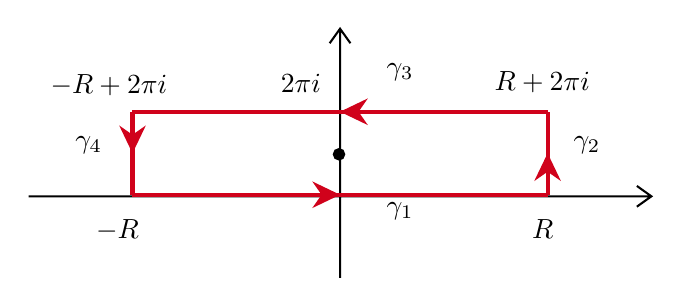
\begin{tikzpicture}[x=0.75pt,y=0.75pt,yscale=-1,xscale=1]
%uncomment if require: \path (0,160); %set diagram left start at 0, and has height of 160

%Shape: Axis 2D [id:dp6952694616964656] 
\draw  (150,110.75) -- (450,110.75)(300,30) -- (300,150) (443,105.75) -- (450,110.75) -- (443,115.75) (295,37) -- (300,30) -- (305,37)  ;
%Shape: Circle [id:dp010000296023957134] 
\draw  [fill={rgb, 255:red, 0; green, 0; blue, 0 }  ,fill opacity=1 ] (297,90.5) .. controls (297,89.12) and (298.12,88) .. (299.5,88) .. controls (300.88,88) and (302,89.12) .. (302,90.5) .. controls (302,91.88) and (300.88,93) .. (299.5,93) .. controls (298.12,93) and (297,91.88) .. (297,90.5) -- cycle ;
%Straight Lines [id:da3282163126700619] 
\draw [color={rgb, 255:red, 208; green, 2; blue, 27 }  ,draw opacity=1 ][line width=1.5]    (200,70) -- (200,110) ;
\draw [shift={(200,90)}, rotate = 270] [fill={rgb, 255:red, 208; green, 2; blue, 27 }  ,fill opacity=1 ][line width=0.08]  [draw opacity=0] (13.4,-6.43) -- (0,0) -- (13.4,6.44) -- (8.9,0) -- cycle    ;
%Straight Lines [id:da8194840593110315] 
\draw [color={rgb, 255:red, 208; green, 2; blue, 27 }  ,draw opacity=1 ][line width=1.5]    (400,110) -- (400,70) ;
\draw [shift={(400,90)}, rotate = 450] [fill={rgb, 255:red, 208; green, 2; blue, 27 }  ,fill opacity=1 ][line width=0.08]  [draw opacity=0] (13.4,-6.43) -- (0,0) -- (13.4,6.44) -- (8.9,0) -- cycle    ;
%Straight Lines [id:da32015283387712334] 
\draw [color={rgb, 255:red, 208; green, 2; blue, 27 }  ,draw opacity=1 ][line width=1.5]    (400,70) -- (200,70) ;
\draw [shift={(300,70)}, rotate = 360] [fill={rgb, 255:red, 208; green, 2; blue, 27 }  ,fill opacity=1 ][line width=0.08]  [draw opacity=0] (13.4,-6.43) -- (0,0) -- (13.4,6.44) -- (8.9,0) -- cycle    ;
%Straight Lines [id:da18099188002221434] 
\draw [color={rgb, 255:red, 208; green, 2; blue, 27 }  ,draw opacity=1 ][line width=1.5]    (200,110) -- (400,110) ;
\draw [shift={(300,110)}, rotate = 180] [fill={rgb, 255:red, 208; green, 2; blue, 27 }  ,fill opacity=1 ][line width=0.08]  [draw opacity=0] (13.4,-6.43) -- (0,0) -- (13.4,6.44) -- (8.9,0) -- cycle    ;

% Text Node
\draw (391,120.4) node [anchor=north west][inner sep=0.75pt]    {$R$};
% Text Node
\draw (181,120.4) node [anchor=north west][inner sep=0.75pt]    {$-R$};
% Text Node
\draw (373,49.4) node [anchor=north west][inner sep=0.75pt]    {$R+2\pi i$};
% Text Node
\draw (159,50.4) node [anchor=north west][inner sep=0.75pt]    {$-R+2\pi i$};
% Text Node
\draw (270,50.4) node [anchor=north west][inner sep=0.75pt]    {$2\pi i$};
% Text Node
\draw (321,112.4) node [anchor=north west][inner sep=0.75pt]    {$\gamma _{1}$};
% Text Node
\draw (411,80.4) node [anchor=north west][inner sep=0.75pt]    {$\gamma _{2}$};
% Text Node
\draw (321,45.4) node [anchor=north west][inner sep=0.75pt]    {$\gamma _{3}$};
% Text Node
\draw (171,80.4) node [anchor=north west][inner sep=0.75pt]    {$\gamma _{4}$};


\end{tikzpicture}
\end{figure}
\FloatBarrier

\begin{equation*}
\int _{\gamma _{R}} f\left( z\right) dz=2\pi i\left[\mathrm{Res}\left( f,\pi i\right)\right] =2\pi i\left[\frac{e^{\alpha z}}{e^{z}}\right]_{z=\pi i} =-2\pi ie^{i\alpha \pi }
\end{equation*}
Vediamo quanto valgono i vari integrali. Quello su $\gamma _{2}$ (e analogamente su $\gamma _{4}$)
\begin{align*}
\left| \int _{\gamma _{2}} f\left( z\right) dz\right|  & =\left\{\gamma _{2} :x=R,y\in \left[ 0,2\pi \right] ,dz=idy\right\} =\\
 & =\left| \int ^{2\pi }_{0}\frac{e^{\alpha R+i\alpha y}}{1+e^{R+iy}} idy\right| \leqslant \int ^{2\pi }_{0}\frac{e^{\alpha R}}{e^{R} -1} dy=2\pi \frac{e^{\alpha R}}{e^{R} -1}\xrightarrow{R\rightarrow +\infty } 0
\end{align*}
Quello su $\gamma _{3}$
\begin{align*}
\int _{\gamma _{3}} f\left( z\right) dz & =\left\{z=x+2\pi i\right\} =\\
 & =-\int ^{R}_{-R}\frac{e^{\alpha x} e^{i2\pi \alpha }}{1+e^{x+2\pi i}} dx=-e^{i2\pi \alpha }\int ^{R}_{-R} f\left( x\right) dx
\end{align*}
quindi
\begin{align*}
\int _{\gamma _{R}} f\left( z\right) dz & \rightarrow -2\pi ie^{i\alpha \pi }\\
\int ^{R}_{-R} f\left( x\right) dx-e^{i2\pi \alpha }\int ^{R}_{-R} f\left( x\right) dx+\underbrace{\int _{\gamma _{2}} f\left( z\right) dz+\int _{\gamma _{4}} f\left( z\right) dz}_{\rightarrow 0} & \rightarrow -2\pi ie^{i\alpha \pi }\\
\left( 1-e^{i2\pi \alpha }\right)\int ^{R}_{-R} f\left( x\right) dx & \rightarrow -2\pi ie^{i\alpha \pi }
\end{align*}
in conclusione
\begin{equation*}
\int _{\mathbb{R}} f\left( x\right) dx=\frac{2\pi ie^{i\alpha \pi }}{e^{i2\pi \alpha } -1} =2\pi i\frac{e^{i\alpha \pi }}{e^{2i\alpha \pi } -1} \cdotp \frac{e^{-i\alpha \pi }}{e^{-i\alpha \pi }} =2\pi i\frac{1}{e^{i\alpha \pi } -e^{-i\alpha \pi }} =\frac{\pi }{\sin\left( \alpha \pi \right)}
\end{equation*}
\chapter{Esercitazione 3 - Potrich}
\ParteEsercizi
\Esercizio{}

Calcolare, al variare di $R >0$
\begin{equation*}
I_{R} =\int _{\gamma _{R}}\frac{\left( z+1\right) e^{\pi z}}{z^{2}\left( z^{2} +1\right)} dz
\end{equation*}
dove
\begin{equation*}
\gamma _{R} :\left| z-1-i\right| =R
\end{equation*}
percorsa positivamente.
\Esercizio{}

Vediamo alcuni integrali reali con metodi di analisi complessa.
\begin{equation*}
I=\boxed{\int ^{2\pi }_{0} R\left(\cos t,\sin t\right) dt}
\end{equation*}
dove $R$ si intende una funzione razionale.
\begin{equation*}
I=\left\{\begin{array}{ c c }
z=e^{it} & \cos t=\frac{e^{it} +e^{-it}}{2}\\
dz=ie^{it} dt & \sin t=\frac{e^{it} -e^{-it}}{2i}
\end{array}\right\} =\int _{\left| z\right| =1} R\left(\frac{z+z^{-1}}{2} ,\frac{z-z^{-1}}{2i}\right)\frac{1}{iz} dz
\end{equation*}
Calcolare
\begin{equation*}
\int ^{2\pi }_{0}\frac{1}{3+\sin t} dt
\end{equation*}
\Esercizio{}

Vediamo una seconda tipologia di integrali
\begin{equation*}
\boxed{\int ^{+\infty }_{-\infty } R\left( x\right) dx} \ \ \ \text{oppure} \ \ \ \ \boxed{\int ^{+\infty }_{-\infty } R\left( x\right)\left\{\begin{array}{ c }
e^{ix}\\
\cos x\\
\sin x
\end{array}\right\} dx}
\end{equation*}
Per risolverli basta porre $f\left( z\right) =R\left( z\right)$ oppure $f\left( z\right) =R\left( z\right) e^{iz}$ e si integra sui semicerchi, infine si fa tendere $R\rightarrow +\infty $.

Se ci fossero poli sull'asse reale devo fare dei morsi e applicare il seguente Lemma. Si fa quindi tendere $\varepsilon \rightarrow 0^{+}$ e $R\rightarrow +\infty $.
\begin{theorem}
[Lemma del cerchio piccolo] Sia $f\in \mathcal{H}\left( D\left( z_{0} ,r\right) \setminus \left\{z_{0}\right\}\right)$, sia $z_{0}$ un polo semplice per $f$, sia $\varphi _{\varepsilon }\left( t\right) =z_{0} +\varepsilon e^{it}$ con $t\in \left[ \alpha ,\beta \right]$. Allora
\begin{equation*}
\lim _{\varepsilon \rightarrow 0^{+}}\int _{\varphi _{\varepsilon }} f\left( z\right) dz=\left( \beta -\alpha \right) i\cdotp \mathrm{Res}\left( f,z_{0}\right)
\end{equation*}
\end{theorem}
\begin{figure}[htpb]
	\centering
\tikzset{every picture/.style={line width=0.75pt}} %set default line width to 0.75pt        

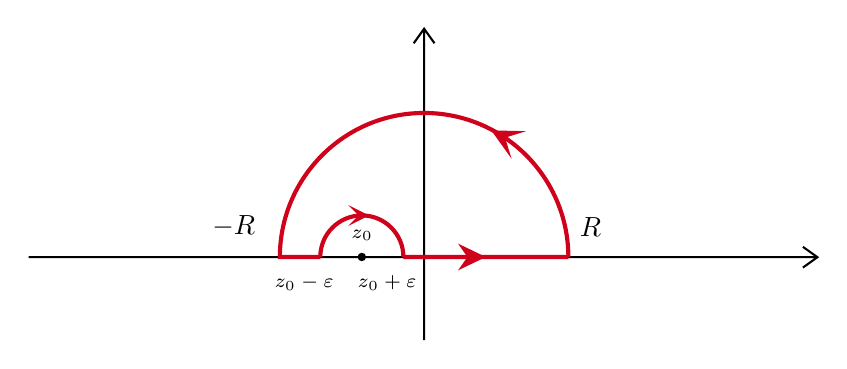
\begin{tikzpicture}[x=0.75pt,y=0.75pt,yscale=-1,xscale=1]
%uncomment if require: \path (0,169); %set diagram left start at 0, and has height of 169

%Shape: Axis 2D [id:dp21276168492453773] 
\draw  (110,120.09) -- (490,120.09)(300.5,10) -- (300.5,160) (483,115.09) -- (490,120.09) -- (483,125.09) (295.5,17) -- (300.5,10) -- (305.5,17)  ;
%Shape: Arc [id:dp9066154861810967] 
\draw  [draw opacity=0][line width=1.5]  (231,120.09) .. controls (231,120.09) and (231,120.09) .. (231,120.09) .. controls (231,81.71) and (262.12,50.59) .. (300.5,50.59) .. controls (338.88,50.59) and (370,81.71) .. (370,120.09) -- (300.5,120.09) -- cycle ; \draw  [color={rgb, 255:red, 208; green, 2; blue, 27 }  ,draw opacity=1 ][line width=1.5]  (231,120.09) .. controls (231,120.09) and (231,120.09) .. (231,120.09) .. controls (231,81.71) and (262.12,50.59) .. (300.5,50.59) .. controls (338.88,50.59) and (370,81.71) .. (370,120.09) ;
%Shape: Arc [id:dp2361543100002761] 
\draw  [draw opacity=0][line width=1.5]  (250.48,119.98) .. controls (250.48,119.98) and (250.48,119.98) .. (250.48,119.98) .. controls (250.48,108.93) and (259.44,99.96) .. (270.5,99.96) .. controls (281.56,99.96) and (290.52,108.93) .. (290.52,119.98) -- (270.5,119.98) -- cycle ; \draw  [color={rgb, 255:red, 208; green, 2; blue, 27 }  ,draw opacity=1 ][line width=1.5]  (250.48,119.98) .. controls (250.48,119.98) and (250.48,119.98) .. (250.48,119.98) .. controls (250.48,108.93) and (259.44,99.96) .. (270.5,99.96) .. controls (281.56,99.96) and (290.52,108.93) .. (290.52,119.98) ;
%Shape: Circle [id:dp06145462056718265] 
\draw  [fill={rgb, 255:red, 0; green, 0; blue, 0 }  ,fill opacity=1 ] (269,119.98) .. controls (269,119.15) and (269.67,118.48) .. (270.5,118.48) .. controls (271.33,118.48) and (272,119.15) .. (272,119.98) .. controls (272,120.81) and (271.33,121.48) .. (270.5,121.48) .. controls (269.67,121.48) and (269,120.81) .. (269,119.98) -- cycle ;
\draw  [draw opacity=0][fill={rgb, 255:red, 208; green, 2; blue, 27 }  ,fill opacity=1 ] (342.64,72.63) -- (332.87,59) -- (349.63,59.36) -- (339.5,62.5) -- cycle ;
%Straight Lines [id:da8537685439706526] 
\draw [color={rgb, 255:red, 208; green, 2; blue, 27 }  ,draw opacity=1 ][line width=1.5]    (230,120) -- (250.48,119.98) ;
%Straight Lines [id:da3820014294051135] 
\draw [color={rgb, 255:red, 208; green, 2; blue, 27 }  ,draw opacity=1 ][line width=1.5]    (290.52,119.98) -- (370,120) ;
\draw [shift={(330.26,119.99)}, rotate = 180.01] [fill={rgb, 255:red, 208; green, 2; blue, 27 }  ,fill opacity=1 ][line width=0.08]  [draw opacity=0] (13.4,-6.43) -- (0,0) -- (13.4,6.44) -- (8.9,0) -- cycle    ;
\draw  [draw opacity=0][fill={rgb, 255:red, 208; green, 2; blue, 27 }  ,fill opacity=1 ] (264,95) -- (274,100) -- (264,105) -- (269,100) -- cycle ;

% Text Node
\draw (197,98.4) node [anchor=north west][inner sep=0.75pt]    {$-R$};
% Text Node
\draw (374,99.4) node [anchor=north west][inner sep=0.75pt]    {$R$};
% Text Node
\draw (227,127.4) node [anchor=north west][inner sep=0.75pt]  [font=\scriptsize]  {$z_{0} -\varepsilon $};
% Text Node
\draw (267,127.4) node [anchor=north west][inner sep=0.75pt]  [font=\scriptsize]  {$z_{0} +\varepsilon $};
% Text Node
\draw (264,105.4) node [anchor=north west][inner sep=0.75pt]  [font=\scriptsize]  {$z_{0}$};


\end{tikzpicture}
\end{figure}
\FloatBarrier
Calcolare
\begin{equation*}
I_{\alpha ,k} =\int ^{+\infty }_{-\infty }\frac{x^{k}}{\alpha ^{2} +x^{2k}} dx\ \ \ \ \alpha  >0,k\in \mathbb{N}
\end{equation*}
\Esercizio{}

Calcolare
\begin{equation*}
I=\int ^{+\infty }_{0}\frac{\sin x}{x} dx
\end{equation*}
\Esercizio{}

Calcolare
\begin{equation*}
\int ^{+\infty }_{-\infty }\frac{\sin\left( \pi x\right)}{\left( x-3\right)\left( x^{2} -2x+2\right)} dx
\end{equation*}
\Esercizio{}

Vediamo una terza tipologia di integrali
\begin{equation*}
\boxed{\int ^{+\infty }_{-\infty } R\left( e^{x}\right)\left\{\begin{array}{ c }
1\\
e^{ix}
\end{array}\right\} dx}
\end{equation*}
Si risolvono integrando sui rettangoli, facendo degli opportuni morsi se e dove necessario.

Calcolare
\begin{equation*}
\int ^{+\infty }_{-\infty }\frac{\cos x}{\cosh x} dx
\end{equation*}
\ParteSoluzioni
\Soluzione

$f\in \mathcal{H}(\mathbb{C} \setminus \{0,\pm i\})$ dove $\pm i$ sono poli semplici, mentre $0$ è un polo del II ordine. 


\begin{figure}[htpb]
	\centering
\tikzset{every picture/.style={line width=0.75pt}} %set default line width to 0.75pt        

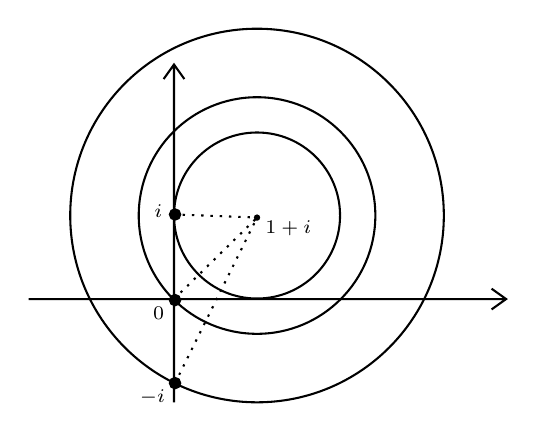
\begin{tikzpicture}[x=0.75pt,y=0.75pt,yscale=-1,xscale=1]
%uncomment if require: \path (0,205); %set diagram left start at 0, and has height of 205

%Shape: Axis 2D [id:dp9998288753339848] 
\draw  (180,140.25) -- (410,140.25)(250,27.25) -- (250,190) (403,135.25) -- (410,140.25) -- (403,145.25) (245,34.25) -- (250,27.25) -- (255,34.25)  ;
%Straight Lines [id:da12445530205724542] 
\draw  [dash pattern={on 0.84pt off 2.51pt}]  (291,101) -- (250.5,99.5) ;
%Shape: Ellipse [id:dp7674970843501638] 
\draw  [fill={rgb, 255:red, 0; green, 0; blue, 0 }  ,fill opacity=1 ] (248,140.75) .. controls (248,139.37) and (249.12,138.25) .. (250.5,138.25) .. controls (251.88,138.25) and (253,139.37) .. (253,140.75) .. controls (253,142.13) and (251.88,143.25) .. (250.5,143.25) .. controls (249.12,143.25) and (248,142.13) .. (248,140.75) -- cycle ;
%Shape: Ellipse [id:dp5063104104492224] 
\draw  [fill={rgb, 255:red, 0; green, 0; blue, 0 }  ,fill opacity=1 ] (248,180.75) .. controls (248,179.37) and (249.12,178.25) .. (250.5,178.25) .. controls (251.88,178.25) and (253,179.37) .. (253,180.75) .. controls (253,182.13) and (251.88,183.25) .. (250.5,183.25) .. controls (249.12,183.25) and (248,182.13) .. (248,180.75) -- cycle ;
%Shape: Ellipse [id:dp3475276859167522] 
\draw  [fill={rgb, 255:red, 0; green, 0; blue, 0 }  ,fill opacity=1 ] (248,99.5) .. controls (248,98.12) and (249.12,97) .. (250.5,97) .. controls (251.88,97) and (253,98.12) .. (253,99.5) .. controls (253,100.88) and (251.88,102) .. (250.5,102) .. controls (249.12,102) and (248,100.88) .. (248,99.5) -- cycle ;
%Shape: Circle [id:dp9945561623234371] 
\draw   (250,100) .. controls (250,77.91) and (267.91,60) .. (290,60) .. controls (312.09,60) and (330,77.91) .. (330,100) .. controls (330,122.09) and (312.09,140) .. (290,140) .. controls (267.91,140) and (250,122.09) .. (250,100) -- cycle ;
%Shape: Circle [id:dp6603014030673247] 
\draw   (233,100) .. controls (233,68.52) and (258.52,43) .. (290,43) .. controls (321.48,43) and (347,68.52) .. (347,100) .. controls (347,131.48) and (321.48,157) .. (290,157) .. controls (258.52,157) and (233,131.48) .. (233,100) -- cycle ;
%Shape: Circle [id:dp8201517506911262] 
\draw   (200,100) .. controls (200,50.29) and (240.29,10) .. (290,10) .. controls (339.71,10) and (380,50.29) .. (380,100) .. controls (380,149.71) and (339.71,190) .. (290,190) .. controls (240.29,190) and (200,149.71) .. (200,100) -- cycle ;
%Shape: Ellipse [id:dp147014916814163] 
\draw  [fill={rgb, 255:red, 0; green, 0; blue, 0 }  ,fill opacity=1 ] (289,101) .. controls (289,100.45) and (289.45,100) .. (290,100) .. controls (290.55,100) and (291,100.45) .. (291,101) .. controls (291,101.55) and (290.55,102) .. (290,102) .. controls (289.45,102) and (289,101.55) .. (289,101) -- cycle ;
%Straight Lines [id:da32148847298984107] 
\draw  [dash pattern={on 0.84pt off 2.51pt}]  (250,140.25) -- (290,101) ;
%Straight Lines [id:da4835195406384667] 
\draw  [dash pattern={on 0.84pt off 2.51pt}]  (250.5,180.75) -- (290,101) ;

% Text Node
\draw (292.5,100.9) node [anchor=north west][inner sep=0.75pt]  [font=\scriptsize]  {$1+i$};
% Text Node
\draw (232,182.4) node [anchor=north west][inner sep=0.75pt]  [font=\scriptsize]  {$-i$};
% Text Node
\draw (238.5,142.4) node [anchor=north west][inner sep=0.75pt]  [font=\scriptsize]  {$0$};
% Text Node
\draw (239,93.4) node [anchor=north west][inner sep=0.75pt]  [font=\scriptsize]  {$i$};


\end{tikzpicture}
\end{figure}
\FloatBarrier

Calcoliamo i residui
\begin{gather*}
\mathrm{Res}\left( f,0\right) =\lim _{z\rightarrow 0}\frac{d}{dz}\left(\left( z-0\right)^{2}\frac{\left( z+1\right) e^{\pi z}}{z^{2}\left( z^{2} +1\right)}\right) =\lim _{z\rightarrow 0}\frac{d}{dz}\frac{\left( z+1\right) e^{\pi z}}{z^{2} +1} =\dotsc =1+\pi \\
\mathrm{Res}\left( f,i\right) =\lim _{z\rightarrow i}\left( z-i\right) f\left( z\right) =\lim _{z\rightarrow i}\frac{\left( z+1\right) e^{\pi z}}{z^{2}\left( z+i\right)} =\dotsc =\frac{1+i}{2i}\\
\mathrm{Res}\left( f,-i\right) =\lim _{z\rightarrow -i}\left( z+i\right) f\left( z\right) =\dotsc =-\frac{1-i}{2i}
\end{gather*}
Le distanze dei punti singolari di $f$ dal centro della curva $\gamma _{R}$ sono
\begin{gather*}
d\left( i,i+1\right) =\left| i-1-i\right| =1\\
d\left( 0,i+1\right) =\left| 1+i\right| =\sqrt{2}\\
d\left( -i,i+1\right) =\left| -i-1-i\right| =\left| -2i-1\right| =\sqrt{5}
\end{gather*}
Allora
\begin{itemize}
\item se $0< R< 1$ per il teorema dei residui\begin{equation*}
I_{R} =0
\end{equation*}
\item se $1< R< \sqrt{2}$ $f$ è olomorfa all'interno di $\gamma _{R}$ tranne che in $z=i$\begin{equation*}
I_{R} =2\pi i\cdotp \mathrm{Res}\left( f,i\right) =\left( 1+i\right) \pi 
\end{equation*}
\item se $\sqrt{2} < R< \sqrt{5}$ $f$ è olomorfa all'interno di $\gamma _{R}$ tranne che in $z=i$ e $z=0$\begin{equation*}
I_{R} =2\pi i\cdotp \left[\mathrm{Res}\left( f,i\right) +\mathrm{Res}\left( f,0\right)\right] =\pi +i\pi \left( 3 +2\pi\right)
\end{equation*}
\item se $R> \sqrt{5}$ tutte le singolarità sono all'interno di $\gamma _{R}$. $f$ è olomorfa all'interno di $\gamma _{R}$ tranne che in $z=\pm i$ e $z=0$\begin{equation*}
I_{R} =2\pi i\cdotp \left[\mathrm{Res}\left( f,0\right) +\mathrm{Res}\left( f,i\right) +\mathrm{Res}\left( f,-i\right)\right] = i2\pi (2+\pi )
\end{equation*}
\end{itemize}

Per $R=1,\sqrt{2} ,\sqrt{5}$, $I_{R}$ non può essere calcolato perché $\gamma _{R}$ passa attraverso una singolarità
\Soluzione
\begin{align*}
\int ^{2\pi }_{0}\frac{1}{3+\sin t} dt & =\int _{\left| z\right| =1}\frac{1}{3+\frac{z-z^{-1}}{2i}}\frac{1}{iz} dz\\
 & =\int _{\left| z\right| =1}\frac{2\cancel{iz}}{z^{2} +6iz-1}\frac{1}{\cancel{iz}} dz=2\int _{\left| z\right| =1}\frac{i}{z^{2} +6iz-1} dz
\end{align*}
Le singolarità sono
\begin{equation*}
z^{2} +6iz-1=0\ \ \Leftrightarrow \ \ \begin{cases}
z_{1} =i\left( -3-2\sqrt{2}\right)\\
z_{2} =i\left( -3+2\sqrt{2}\right)
\end{cases}
\end{equation*}
di cui solo $z_{2}$ sta dentro il cerchio unitario
\begin{equation*}
2\int _{\left| z\right| =1}\frac{i}{z^{2} +6iz-1} dz=2\cdotp 2\pi i\cdotp \mathrm{Res}\left( f,i\left( -3+2\sqrt{2}\right)\right)
\end{equation*}
ricordando che è un polo semplice
\begin{equation*}
4\pi i\cdotp \mathrm{Res}\left( f,i\left( -3+2\sqrt{2}\right)\right) =4\pi i\lim\limits _{z\rightarrow i\left( -3+2\sqrt{2}\right)}\left[ z-i\left( -3+2\sqrt{2}\right)\right] f\left( z\right) =\dotsc =\frac{\pi }{\sqrt{2}}
\end{equation*}
\Soluzione
\begin{equation*}
I_{\alpha ,k} =\int ^{+\infty }_{-\infty }\frac{x^{k}}{\alpha ^{2} +x^{2k}} dx\ \ \ \ \alpha  >0,k\in \mathbb{N}
\end{equation*}
Per $x\rightarrow \pm \infty $ si ha $f\left( x\right) \sim \frac{1}{x^{k}}$, che è integrabile in un intorno di $\pm \infty $ se e solo se $k >1$. Quindi $I_{\alpha ,k}$ esiste per $k\in \mathbb{N} ,k\geqslant 2$.

Se $k$ è dispari allora $f$ è dispari e $I_{\alpha ,k} =0$

Se $k$ è pari, con $k\geqslant 2$, poniamo
\begin{equation*}
f\left( z\right) =\frac{z^{k}}{\alpha ^{2} +z^{2k}}
\end{equation*}
Le singolarità si trovano ponendo
\begin{equation*}
z^{2k} =-\alpha ^{2} =\alpha ^{2} e^{\pi i} \ \ \Rightarrow \ \ z_{j} =\alpha ^{\frac{1}{k}} e^{i\frac{\pi +2j\pi }{2k}} \ \ \ \ 0\leqslant j\leqslant k-1
\end{equation*}
allora per il teorema dei residui
\begin{equation*}
\int _{\gamma _{R}} f\left( z\right) dz=\int _{\sigma } f\left( z\right) dz+\int _{\varphi } f\left( z\right) dz=2\pi i\cdotp \sum\limits ^{k-1}_{j=0}\mathrm{Res}\left( f,z_{j}\right)
\end{equation*}
Nello specifico il pezzo su $\sigma $ tende proprio al nostro integrale
\begin{equation*}
\int _{\sigma } f\left( z\right) dz=\left\{z=t,t\in \left[ -R,R\right]\right\} =\int ^{R}_{-R} f\left( t\right) dt\xrightarrow{R\rightarrow +\infty } I_{\alpha ,k}
\end{equation*}
Verifichiamo che
\begin{equation*}
\int _{\varphi } f\left( z\right) dz\rightarrow 0
\end{equation*}
Infatti
\begin{align*}
\left| \int _{\varphi } f\left( z\right) dz\right|  & =\left\{z=Re^{it} ,t\in \left[ 0,\pi \right]\right\} =\left| \int ^{\pi }_{0}\frac{R^{k} e^{ikt}}{\alpha ^{2} +R^{2k} e^{i2kt}} Rie^{it} dt\right| \\
 & \leqslant \int ^{\pi }_{0}\frac{\left| R^{k} e^{ikt}\right| }{\left| \alpha ^{2} +R^{2k} e^{i2kt}\right| }\left| Rie^{it}\right| dt\leqslant \int ^{\pi }_{0}\frac{R^{k+1}}{R^{2k} -\alpha ^{2}} dt\xrightarrow{R\rightarrow +\infty } 0
\end{align*}
dove è stata usata la disuguaglianza triangolare
\begin{nb}
[Disuguaglianza triangolare] Per maggiorazioni e minorazioni ecco la forma più generale della disuguaglianza del triangolo
\begin{equation*}
\left| \left| a\right| -\left| b\right| \right| \leqslant \left| a\pm b\right| \leqslant \left| a\right| +\left| b\right| 
\end{equation*}
\end{nb}

\Soluzione
\begin{equation*}
I=\int ^{+\infty }_{0}\frac{\sin x}{x} dx=\frac{1}{2}\int ^{+\infty }_{-\infty }\frac{\sin x}{x} dx=\frac{1}{2}\mathrm{Im}\left( J\right) \ \ \ \ \ \ \ \ J=\int ^{+\infty }_{-\infty }\frac{e^{ix}}{x} dx
\end{equation*}
Posto $f\left( z\right) =\frac{e^{iz}}{z}$, $f\in \mathcal{H}\left(\mathbb{C} \setminus \left\{0\right\}\right)$. In questo caso devo fare un \textit{morso} in corrispondenza dello $0$.
\begin{equation*}
J=\lim _{\varepsilon \rightarrow 0^{+} ,R\rightarrow +\infty }\int _{\left[ -R,R\right] \setminus \left( -\varepsilon ,\varepsilon \right)}\frac{e^{iz}}{z} dz
\end{equation*}
Per il teorema dell'integrale nullo di Cauchy
\begin{equation*}
0=\int _{\gamma _{R,\varepsilon }} f\left( z\right) dz=\int _{\sigma _{1} \cup \sigma _{2}} f\left( z\right) dz+\int _{\psi } f\left( z\right) dz+\int _{\varphi } f\left( z\right) dz
\end{equation*}
Analizziamo i vari pezzi
\begin{equation*}
\int _{\sigma _{1} \cup \sigma _{2}} f\left( z\right) dz=\left\{z=t,t\in \left[ -R,-\varepsilon \right) \cup \left( \varepsilon ,R\right]\right\} =\int _{\left[ -R,R\right] \setminus \left( -\varepsilon ,\varepsilon \right)}\frac{e^{it}}{t} dt\xrightarrow[\varepsilon \rightarrow 0^{+}]{R\rightarrow +\infty } J
\end{equation*}
il morso:
\begin{equation*}
\int _{\psi } f\left( z\right) dz\xrightarrow{\varepsilon \rightarrow 0^{+}}\left( \beta -\alpha \right) \cdotp \mathrm{Res}\left( f,0\right) =\left( 0-\pi \right) i\cdotp \mathrm{Res}\left( f,0\right) =-\pi i\frac{e^{0}}{1} =-\pi i
\end{equation*}
mentre il semicerchio grande:
\begin{align*}
\left| \int _{\varphi } f\left( z\right) dz\right|  & =\left\{z=Re^{it} ,dz=Rie^{it} dt\right\} =\left| \int ^{\pi }_{0}\frac{e^{iRe^{it}}}{\cancel{Re^{it}}} i\cancel{Re^{it}} dt\right| \\
 & \leqslant \int ^{\pi }_{0}\left| e^{iRe^{it}}\right| dt=\left\{\left| e^{z}\right| =e^{\mathrm{Re}\left( z\right)}\right\}\\
 & =\int ^{\pi }_{0} e^{-R\sin t} dt=2\int ^{\frac{\pi }{2}}_{0} e^{-R\sin t} dt\leqslant 2\int ^{\frac{\pi }{2}}_{0} e^{-\frac{2Rt}{\pi }} dt\\
 & =\frac{\pi }{R}\left( 1-e^{-R}\right) \leqslant \frac{\pi }{R}\xrightarrow{R\rightarrow +\infty } 0
\end{align*}
allora
\begin{equation*}
0=J-\pi i+0\ \ \ \ \Rightarrow \ \ \ \ J=\pi i\ \ \ \ \Rightarrow \ \ \ \ I=\frac{1}{2}\mathrm{Im}\left( J\right) =\frac{\pi }{2}
\end{equation*}
\Soluzione

Dobbiamo calcolare
\begin{equation*}
\int ^{+\infty }_{-\infty }\frac{\sin\left( \pi x\right)}{\left( x-3\right)\left( x^{2} -2x+2\right)} dx
\end{equation*}
poniamo
\begin{equation*}
f\left( z\right) =\frac{e^{i\pi z}}{\left( z-3\right)\left( z^{2} -2z+2\right)}
\end{equation*}
$f\in \mathcal{H}\left(\mathbb{C} \setminus \left\{3,1\pm i\right\}\right)$, uno di essi si trova proprio sulla retta reale, pertanto lì faremo un morso.
\begin{align*}
\int _{\gamma _{R,\varepsilon }} f\left( z\right) dz & =2\pi i\cdotp \mathrm{Res}\left( f,1+i\right) =2\pi i\cdotp \lim _{z\rightarrow 1+i} f\left( z\right)\left( z-\left( 1+i\right)\right) =\\
 & =2\pi i\cdotp \lim _{z\rightarrow 1+i}\frac{e^{\pi iz}}{\left( z-3\right)\left( z-1+i\right)} =\dotsc =\frac{\pi e^{-\pi }}{5}\left( 2+i\right)
\end{align*}
ma questo integrale possiamo vederlo come la somma di tre pezzi
\begin{equation*}
\int _{\gamma _{R,\varepsilon }} f\left( z\right) dz=\int _{\left( -R,3-\varepsilon \right) \cup \left( 3+\varepsilon ,R\right)} f\left( z\right) dz+\int _{\psi } f\left( z\right) dz+\int _{\varphi } f\left( z\right) dz
\end{equation*}
di cui il primo tende proprio all'integrale che vogliamo calcolare
\begin{equation*}
\int _{\left( -R,3-\varepsilon \right) \cup \left( 3+\varepsilon ,R\right)} f\left( z\right) dz\xrightarrow[\varepsilon \rightarrow 0^{+}]{R\rightarrow +\infty }\int ^{+\infty }_{-\infty }\frac{e^{i\pi z}}{\left( x-3\right)\left( x^{2} -2x+2\right)} dx
\end{equation*}
occupiamoci del pezzo sul morso sfruttando il Lemma del cerchio piccolo
\begin{align*}
\lim _{\varepsilon \rightarrow 0^{+}}\int _{\psi } f\left( z\right) dz & =-\pi i\cdotp \mathrm{Res}\left( f,3\right)\\
 & =-\pi i\cdotp \lim _{z\rightarrow 3} f\left( z\right)\left( z-3\right) =-\pi i\cdotp \lim _{z\rightarrow 3}\frac{e^{i\pi z}}{z^{2} -2z+2} =\dotsc =\frac{\pi i}{5}
\end{align*}
ed infine del semicerchio grande
\begin{align*}
\left| \int _{\varphi } f\left( z\right) dz\right|  & =\left\{z=Re^{it} ,dz=Rie^{it} dt\right\}\\
 & =\left| \int ^{\pi }_{0}\frac{e^{\pi iRe^{it}}}{\left( Re^{it} -3\right)\left( R^{2} e^{i2t} -2Re^{it} +2\right)} Rie^{it} dt\right| \\
 & \leqslant \int ^{\pi }_{0}\frac{R}{\left( R-3\right)\left( R^{2} -2R-2\right)} dt=\frac{R\pi }{\left( R-3\right)\left( R^{2} -2R-2\right)}\xrightarrow{R\rightarrow +\infty } 0
\end{align*}
quindi
\begin{equation*}
\int ^{+\infty }_{-\infty }\frac{e^{i\pi x}}{\left( x-3\right)\left( x^{2} -2x+2\right)} dx=-\frac{\pi i}{5} +\frac{\pi e^{-\pi }}{5}\left( 2+i\right)
\end{equation*}
ma l'integrale di partenza è proprio la parte immaginaria di questo integrale
\begin{equation*}
\int ^{+\infty }_{-\infty }\frac{\sin\left( \pi x\right)}{\left( x-3\right)\left( x^{2} -2x+2\right)} dx=\mathrm{Im}\left[ -\frac{\pi i}{5} +\frac{\pi e^{-\pi }}{5}\left( 2+i\right)\right] =\frac{\pi }{5}\left( e^{-\pi } -1\right)
\end{equation*}
\Soluzione

Dobbiamo calcolare
\begin{equation*}
\int ^{+\infty }_{-\infty }\frac{\cos x}{\cosh x} dx
\end{equation*}
consideriamo
\begin{equation*}
f\left( z\right) =\frac{e^{iz}}{\cosh z}
\end{equation*}
il cui denominatore si annulla in
\begin{gather*}
\cosh z=0=\frac{e^{z} +e^{-z}}{2} \ \ \Leftrightarrow \ \ e^{2z} =-1\ \ \Leftrightarrow \ \ 2z=\log\left| -1\right| +i\arg\left( -1\right)\\
\Leftrightarrow \ \ 2z=0+i\left( \pi +2k\pi \right) ,k\in \mathbb{Z} \ \ \Leftrightarrow \ \ z=\frac{\pi i}{2} +k\pi 
\end{gather*}
Integriamo sul rettangolo che contiene il residuo in $\pi i/2$
\begin{equation*}
\int _{\gamma _{R}} f\left( z\right) dz=2\pi i\cdotp \mathrm{Res}\left( f,\frac{\pi i}{2}\right) =2\pi i\cdotp \left. \frac{e^{iz}}{\sinh}\right| _{z=\frac{\pi i}{2}} =\dotsc =\frac{2\pi }{e^{\frac{\pi }{2}}}
\end{equation*}
il circuito lo possiamo vedere come $4$ lati di un rettangolo, numerati in senso antiorario partendo da quello in basso


\begin{figure}[htpb]
	\centering
\tikzset{every picture/.style={line width=0.75pt}} %set default line width to 0.75pt        

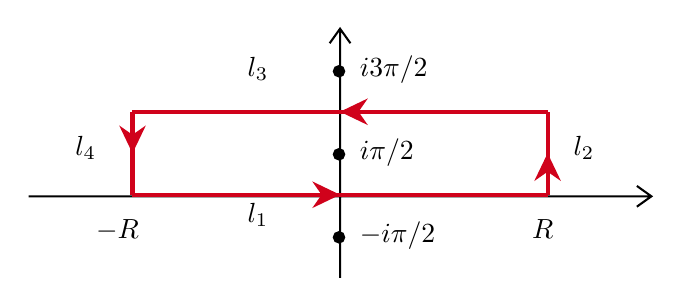
\begin{tikzpicture}[x=0.75pt,y=0.75pt,yscale=-1,xscale=1]
%uncomment if require: \path (0,137); %set diagram left start at 0, and has height of 137

%Shape: Axis 2D [id:dp18751408917716894] 
\draw  (150,90.75) -- (450,90.75)(300,10) -- (300,130) (443,85.75) -- (450,90.75) -- (443,95.75) (295,17) -- (300,10) -- (305,17)  ;
%Shape: Circle [id:dp11440595401764786] 
\draw  [fill={rgb, 255:red, 0; green, 0; blue, 0 }  ,fill opacity=1 ] (297,70.5) .. controls (297,69.12) and (298.12,68) .. (299.5,68) .. controls (300.88,68) and (302,69.12) .. (302,70.5) .. controls (302,71.88) and (300.88,73) .. (299.5,73) .. controls (298.12,73) and (297,71.88) .. (297,70.5) -- cycle ;
%Straight Lines [id:da54907639410711] 
\draw [color={rgb, 255:red, 208; green, 2; blue, 27 }  ,draw opacity=1 ][line width=1.5]    (200,50) -- (200,90) ;
\draw [shift={(200,70)}, rotate = 270] [fill={rgb, 255:red, 208; green, 2; blue, 27 }  ,fill opacity=1 ][line width=0.08]  [draw opacity=0] (13.4,-6.43) -- (0,0) -- (13.4,6.44) -- (8.9,0) -- cycle    ;
%Straight Lines [id:da8839966596936082] 
\draw [color={rgb, 255:red, 208; green, 2; blue, 27 }  ,draw opacity=1 ][line width=1.5]    (400,90) -- (400,50) ;
\draw [shift={(400,70)}, rotate = 450] [fill={rgb, 255:red, 208; green, 2; blue, 27 }  ,fill opacity=1 ][line width=0.08]  [draw opacity=0] (13.4,-6.43) -- (0,0) -- (13.4,6.44) -- (8.9,0) -- cycle    ;
%Straight Lines [id:da5768709170809461] 
\draw [color={rgb, 255:red, 208; green, 2; blue, 27 }  ,draw opacity=1 ][line width=1.5]    (400,50) -- (200,50) ;
\draw [shift={(300,50)}, rotate = 360] [fill={rgb, 255:red, 208; green, 2; blue, 27 }  ,fill opacity=1 ][line width=0.08]  [draw opacity=0] (13.4,-6.43) -- (0,0) -- (13.4,6.44) -- (8.9,0) -- cycle    ;
%Straight Lines [id:da7918111958211875] 
\draw [color={rgb, 255:red, 208; green, 2; blue, 27 }  ,draw opacity=1 ][line width=1.5]    (200,90) -- (400,90) ;
\draw [shift={(300,90)}, rotate = 180] [fill={rgb, 255:red, 208; green, 2; blue, 27 }  ,fill opacity=1 ][line width=0.08]  [draw opacity=0] (13.4,-6.43) -- (0,0) -- (13.4,6.44) -- (8.9,0) -- cycle    ;
%Shape: Circle [id:dp38938153564529987] 
\draw  [fill={rgb, 255:red, 0; green, 0; blue, 0 }  ,fill opacity=1 ] (297,110.5) .. controls (297,109.12) and (298.12,108) .. (299.5,108) .. controls (300.88,108) and (302,109.12) .. (302,110.5) .. controls (302,111.88) and (300.88,113) .. (299.5,113) .. controls (298.12,113) and (297,111.88) .. (297,110.5) -- cycle ;
%Shape: Circle [id:dp5781216178988735] 
\draw  [fill={rgb, 255:red, 0; green, 0; blue, 0 }  ,fill opacity=1 ] (297,30.5) .. controls (297,29.12) and (298.12,28) .. (299.5,28) .. controls (300.88,28) and (302,29.12) .. (302,30.5) .. controls (302,31.88) and (300.88,33) .. (299.5,33) .. controls (298.12,33) and (297,31.88) .. (297,30.5) -- cycle ;

% Text Node
\draw (391,100.4) node [anchor=north west][inner sep=0.75pt]    {$R$};
% Text Node
\draw (181,100.4) node [anchor=north west][inner sep=0.75pt]    {$-R$};
% Text Node
\draw (254,92.4) node [anchor=north west][inner sep=0.75pt]    {$l_{1}$};
% Text Node
\draw (411,60.4) node [anchor=north west][inner sep=0.75pt]    {$l_{2}$};
% Text Node
\draw (254,22.4) node [anchor=north west][inner sep=0.75pt]    {$l_{3}$};
% Text Node
\draw (171,60.4) node [anchor=north west][inner sep=0.75pt]    {$l_{4}$};
% Text Node
\draw (308,61.4) node [anchor=north west][inner sep=0.75pt]    {$i\pi /2$};
% Text Node
\draw (308,101.4) node [anchor=north west][inner sep=0.75pt]    {$-i\pi /2$};
% Text Node
\draw (308,21.4) node [anchor=north west][inner sep=0.75pt]    {$i3\pi /2$};


\end{tikzpicture}
\end{figure}
\FloatBarrier

\begin{equation*}
\int _{\gamma _{R}} f\left( z\right) dz=\int _{l_{1}} f\left( z\right) dz+\int _{l_{2}} f\left( z\right) dz+\int _{l_{3}} f\left( z\right) dz+\int _{l_{4}} f\left( z\right) dz
\end{equation*}
il lato inferiore tende proprio al nostro integrale
\begin{equation*}
\int _{l_{1}} f\left( z\right) dz=\left\{z=t\right\} =\int ^{R}_{-R}\frac{e^{it}}{\cosh t} dt\xrightarrow{R\rightarrow +\infty }\int ^{+\infty }_{-\infty }\frac{e^{it}}{\cosh t} dt
\end{equation*}
mentre il lato superiore tende al nostro integrale moltiplicato per una costante
\begin{align*}
\int _{l_{3}} f\left( z\right) dz & =\left\{z=t+\pi i\right\} =-\int ^{R}_{-R}\frac{e^{i\left( t+\pi i\right)}}{\cosh\left( t+\pi i\right)} dt\\
 & =-\int ^{R}_{-R}\frac{e^{it} e^{-\pi }}{\frac{e^{t+\pi i} +e^{t+\pi i}}{2}} dt=e^{-\pi }\int ^{R}_{-R}\frac{e^{it}}{\cosh t} dt\xrightarrow{R\rightarrow +\infty } e^{-\pi }\int ^{+\infty }_{-\infty }\frac{e^{it}}{\cosh t} dt
\end{align*}
si può dimostrare che i lati verticali tendono a zero
\begin{align*}
\left| \int _{l_{2}} f\left( z\right) dz\right|  & \leqslant \left\{z=R+it,t\in \left[ 0,\pi \right] ,dz=idt\right\} \leqslant \left| \int ^{\pi }_{0}\frac{e^{iR} e^{-t}}{\cosh\left( R+it\right)} idt\right| \\
 & \leqslant \int ^{\pi }_{0}\frac{2e^{-t}}{e^{R} +e^{-R}} dt=\frac{2}{e^{R} +e^{-R}}\int ^{\pi }_{0} e^{-t} dt\xrightarrow{R\rightarrow +\infty } 0
\end{align*}
analogamente
\begin{equation*}
\int _{l_{4}} f\left( z\right) dz\xrightarrow{R\rightarrow +\infty } 0
\end{equation*}
quindi in conclusione
\begin{equation*}
\frac{2\pi }{e^{\frac{\pi }{2}}} =\int ^{+\infty }_{-\infty }\frac{e^{it}}{\cosh t} dt+0+e^{-\pi }\int ^{+\infty }_{-\infty }\frac{e^{it}}{\cosh t} dt+0
\end{equation*}
isoliamo il nostro integrale
\begin{equation*}
\left( 1+e^{-\pi }\right)\int ^{+\infty }_{-\infty }\frac{e^{it}}{\cosh t} d=\frac{2\pi }{e^{\frac{\pi }{2}}} \ \ \Rightarrow \ \ \int ^{+\infty }_{-\infty }\frac{e^{it}}{\cosh t} dt=\frac{2\pi }{\left( 1+e^{-\pi }\right) e^{\frac{\pi }{2}}} =\frac{\pi }{\cosh\left(\frac{\pi }{2}\right)}
\end{equation*}
ma l'integrale di partenza è proprio la parte reale di questo integrale
\begin{equation*}
\int ^{+\infty }_{-\infty }\frac{\cos x}{\cosh x} dx=\mathrm{Re}\left[\int ^{+\infty }_{-\infty }\frac{e^{it}}{\cosh t} dt\right] =\frac{\pi }{\cosh\left(\frac{\pi }{2}\right)}
\end{equation*}
\chapter{Esercitazione 4 - Boella}
\ParteEsercizi
\Esercizio{}

Calcolare il seguente integrale:
\begin{equation*}
\int ^{+\infty }_{0}\frac{\cos (\alpha x)}{x^{2} +\beta ^{2}} dx\ \ \ \ \alpha ,\beta  >0
\end{equation*}
\Esercizio{}

Calcolare il seguente integrale:
\begin{equation*}
\int _{\mathbb{R}}\frac{e^{ix}}{x^{3} +x^{2} +x+1} dx
\end{equation*}
\Esercizio{}

Calcolare l'integrale della funzione polidroma:
\begin{equation*}
\int ^{\infty }_{0}\frac{\sqrt[3]{x}}{x^{2} +4} dx
\end{equation*}
\Esercizio{}

Studiare la convergenza della seguente successione di funzioni:
\begin{equation*}
f_{n} (x)=\frac{\sqrt{n}}{1+(nx)^{2}}
\end{equation*}
\Esercizio{}

Studiare la convergenza della seguente successione di funzioni:
\begin{equation*}
f_{n} (x)=n^{\alpha } \chi _{\left( 0,\frac{1}{n}\right)} (x)
\end{equation*}
\Esercizio{}

Studiare la convergenza della seguente successione di funzioni:
\begin{equation*}
f_{n} (x)=\frac{1-e^{-x}}{x( 1-x)^{1/n}} \chi _{( 0,1)} (x)
\end{equation*}
\ParteSoluzioni
\Soluzione

Ho due vie:
\begin{itemize}
\item Calcolare l'integrale sfruttando le formule di Eulero
\item Farsi furbi (seguiremo questa soluzione)
\end{itemize}

Riconoscendo che la funzione integranda è pari posso scrivere che:
\begin{equation*}
\int ^{+\infty }_{0}\frac{\cos (\alpha x)}{x^{2} +\beta ^{2}} dx\overset{\text{(pari)}}{=}\frac{1}{2}\int _{\mathbb{R}}\frac{\cos (\alpha x)}{x^{2} +\beta ^{2}} dx\overset{\text{(*)}}{=}\frac{1}{2}\left(\int _{\mathbb{R}}\frac{\cos (\alpha x)}{x^{2} +\beta ^{2}} dx+i\int _{\mathbb{R}}\frac{\sin (\alpha x)}{x^{2} +\beta ^{2}} dx\right)
\end{equation*}
Nel passaggio (*) abbiamo sfruttato l'annullamento dell'integrale di una funzione dispari su tutto $\mathbb{R}$. Riconosciamo ora che possiamo riscriverla come:

\begin{equation*}
\frac{1}{2}\int _{\mathbb{R}}\frac{e^{i\alpha x}}{x^{2} +\beta ^{2}} dx
\end{equation*}Prendiamo ora in esame $f(z)=\frac{e^{i\alpha x}}{x^{2} +\beta ^{2}}$, sfruttiamo il Lemma di Jordan ($\alpha  >0$) e il Teorema dei residui, integrando sulla semicirconferenza superiore.
\begin{equation*}
\int _{\gamma _{R}} f( z) dz=2\pi i\cdotp \mathrm{Res}( f,z=i\beta ) =2\pi i\cdotp \left. \frac{e^{i\alpha x}}{2z}\right| _{z=i\beta } =\frac{\pi }{\beta } e^{-\alpha \beta }
\end{equation*}
Per $R\rightarrow +\infty $
\begin{equation*}
\frac{\pi }{\beta } e^{-\alpha \beta } =\int _{\gamma _{R}} =\int ^{R}_{-R} +\cancel{\int _{\sigma _{R}}}\xrightarrow{R\rightarrow +\infty }\int _{\mathbb{R}} f( x) dx\ \ \Rightarrow \ \ \frac{1}{2}\int _{\mathbb{R}}\frac{e^{i\alpha x}}{x^{2} +\beta ^{2}} dx=\frac{\pi e^{-\alpha \beta }}{2\beta }
\end{equation*}
\Soluzione

C'è un asintoto verticale in $x=-1$, quindi non converge.\begin{equation*}
\int _{\mathbb{R}}\frac{e^{ix}}{x^{3} +x^{2} +x+1} dx=\int _{\mathbb{R}}\frac{e^{ix}}{(x^{2} +1)(x+1)} dx
\end{equation*}

Non calcoliamo lui, ma il suo \textit{Valore Principale:} ovvero dobbiamo fare i limiti tutti insieme, non separati. In caso di forme di indecisione $( \infty -\infty )$ potrebbe saltare fuori qualcosa di buono.
\begin{equation*}
( VP)\int _{\mathbb{R}}\frac{e^{ix}}{(x^{2} +1)(x+1)} dx=\lim _{\varepsilon \rightarrow 0^{+} \ R\rightarrow \infty }\left[\int ^{-1-\varepsilon }_{-R} f(x)dx+\int ^{R}_{-1+\varepsilon } f(x)dx\right]
\end{equation*}
Rinfrescate le idee, ora consideriamo come dominio di integrazione una semicirconferenza come raffigurata e scomponiamo l'integrale sulle 4 curve (due tratti curvilinei e due rettilinei, prima e dopo la circonferenza interna).


\begin{figure}[htpb]
	\centering
\tikzset{every picture/.style={line width=0.75pt}} %set default line width to 0.75pt        

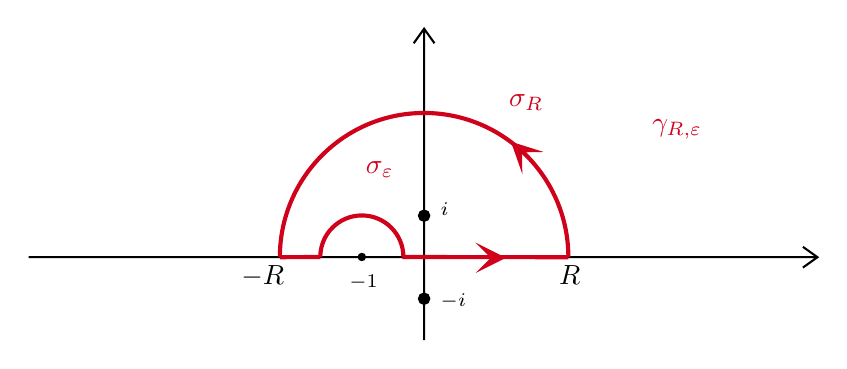
\begin{tikzpicture}[x=0.75pt,y=0.75pt,yscale=-1,xscale=1]
%uncomment if require: \path (0,166); %set diagram left start at 0, and has height of 166

%Shape: Axis 2D [id:dp4597416392621234] 
\draw  (110,120.09) -- (490,120.09)(300.5,10) -- (300.5,160) (483,115.09) -- (490,120.09) -- (483,125.09) (295.5,17) -- (300.5,10) -- (305.5,17)  ;
%Shape: Arc [id:dp48689113730354094] 
\draw  [draw opacity=0][line width=1.5]  (231,120.09) .. controls (231,120.09) and (231,120.09) .. (231,120.09) .. controls (231,81.71) and (262.12,50.59) .. (300.5,50.59) .. controls (338.88,50.59) and (370,81.71) .. (370,120.09) -- (300.5,120.09) -- cycle ; \draw  [color={rgb, 255:red, 208; green, 2; blue, 27 }  ,draw opacity=1 ][line width=1.5]  (231,120.09) .. controls (231,120.09) and (231,120.09) .. (231,120.09) .. controls (231,81.71) and (262.12,50.59) .. (300.5,50.59) .. controls (338.88,50.59) and (370,81.71) .. (370,120.09) ;
%Shape: Arc [id:dp3783656851334405] 
\draw  [draw opacity=0][line width=1.5]  (250.48,119.98) .. controls (250.48,119.98) and (250.48,119.98) .. (250.48,119.98) .. controls (250.48,108.93) and (259.44,99.96) .. (270.5,99.96) .. controls (281.56,99.96) and (290.52,108.93) .. (290.52,119.98) -- (270.5,119.98) -- cycle ; \draw  [color={rgb, 255:red, 208; green, 2; blue, 27 }  ,draw opacity=1 ][line width=1.5]  (250.48,119.98) .. controls (250.48,119.98) and (250.48,119.98) .. (250.48,119.98) .. controls (250.48,108.93) and (259.44,99.96) .. (270.5,99.96) .. controls (281.56,99.96) and (290.52,108.93) .. (290.52,119.98) ;
%Shape: Circle [id:dp8264521136482348] 
\draw  [fill={rgb, 255:red, 0; green, 0; blue, 0 }  ,fill opacity=1 ] (269,119.98) .. controls (269,119.15) and (269.67,118.48) .. (270.5,118.48) .. controls (271.33,118.48) and (272,119.15) .. (272,119.98) .. controls (272,120.81) and (271.33,121.48) .. (270.5,121.48) .. controls (269.67,121.48) and (269,120.81) .. (269,119.98) -- cycle ;
\draw  [draw opacity=0][fill={rgb, 255:red, 208; green, 2; blue, 27 }  ,fill opacity=1 ] (347.82,80) -- (342.34,64.44) -- (358.08,69.39) -- (347.64,69.57) -- cycle ;
\draw  [draw opacity=0][fill={rgb, 255:red, 208; green, 2; blue, 27 }  ,fill opacity=1 ] (325.24,113) -- (340,120.38) -- (325.24,127.76) -- (332.62,120.38) -- cycle ;
%Straight Lines [id:da6476958893771378] 
\draw [color={rgb, 255:red, 208; green, 2; blue, 27 }  ,draw opacity=1 ][line width=1.5]    (231,120.09) -- (250.48,119.98) ;
%Straight Lines [id:da8263168573202715] 
\draw [color={rgb, 255:red, 208; green, 2; blue, 27 }  ,draw opacity=1 ][line width=1.5]    (290,120) -- (370,120.09) ;
%Shape: Circle [id:dp7603714452226784] 
\draw  [fill={rgb, 255:red, 0; green, 0; blue, 0 }  ,fill opacity=1 ] (298,100.09) .. controls (298,98.71) and (299.12,97.59) .. (300.5,97.59) .. controls (301.88,97.59) and (303,98.71) .. (303,100.09) .. controls (303,101.47) and (301.88,102.59) .. (300.5,102.59) .. controls (299.12,102.59) and (298,101.47) .. (298,100.09) -- cycle ;
%Shape: Circle [id:dp46768054307943396] 
\draw  [fill={rgb, 255:red, 0; green, 0; blue, 0 }  ,fill opacity=1 ] (298,140.09) .. controls (298,138.71) and (299.12,137.59) .. (300.5,137.59) .. controls (301.88,137.59) and (303,138.71) .. (303,140.09) .. controls (303,141.47) and (301.88,142.59) .. (300.5,142.59) .. controls (299.12,142.59) and (298,141.47) .. (298,140.09) -- cycle ;

% Text Node
\draw (211,122.4) node [anchor=north west][inner sep=0.75pt]    {$-R$};
% Text Node
\draw (364,122.4) node [anchor=north west][inner sep=0.75pt]    {$R$};
% Text Node
\draw (263,127.4) node [anchor=north west][inner sep=0.75pt]  [font=\scriptsize]  {$-1$};
% Text Node
\draw (409,52.4) node [anchor=north west][inner sep=0.75pt]  [color={rgb, 255:red, 208; green, 2; blue, 27 }  ,opacity=1 ]  {$\gamma _{R,\varepsilon }$};
% Text Node
\draw (271,72.4) node [anchor=north west][inner sep=0.75pt]  [color={rgb, 255:red, 208; green, 2; blue, 27 }  ,opacity=1 ]  {$\sigma _{\varepsilon }$};
% Text Node
\draw (340,40.4) node [anchor=north west][inner sep=0.75pt]  [color={rgb, 255:red, 208; green, 2; blue, 27 }  ,opacity=1 ]  {$\sigma _{R}$};
% Text Node
\draw (307,92.4) node [anchor=north west][inner sep=0.75pt]  [font=\scriptsize]  {$i$};
% Text Node
\draw (307,136.4) node [anchor=north west][inner sep=0.75pt]  [font=\scriptsize]  {$-i$};


\end{tikzpicture}
\end{figure}
\FloatBarrier

\begin{equation*}
\int _{\gamma _{R,\varepsilon }} f(z)dz=2\pi i\cdot \mathrm{Res} (f,z=i)=2\pi i\cdotp \left. \frac{e^{iz}}{3z^{2} +2z+1}\right| _{z=i} =2\pi i\cdotp \frac{e^{-1}}{2i-2}
\end{equation*}
Quando $\varepsilon \rightarrow 0^{+} ,R\rightarrow \infty $
\begin{equation*}
\int _{\gamma _{R,\varepsilon }} =\int ^{-1-\varepsilon }_{-R} +\int _{\sigma _{\varepsilon }} +\int ^{R}_{-1-\varepsilon } +\int _{\sigma _{R}}
\end{equation*}
\begin{theorem}
[Lemma del cerchio piccolo] Sia $f\in \mathcal{H}( D( z_{0} ,r) \setminus \{z_{0}\})$, sia $z_{0}$ un polo semplice per $f$, sia $\varphi _{\varepsilon }( t) =z_{0} +\varepsilon e^{it}$ con $t\in [ \alpha ,\beta ]$. Allora
\begin{equation*}
\lim _{\varepsilon \rightarrow 0^{+}}\int _{\varphi _{\varepsilon }} f( z) dz=( \beta -\alpha ) i\cdotp \mathrm{Res}( f,z_{0})
\end{equation*}
\end{theorem}
Per Jordan, quello su $\sigma _{R}$ tende a $0$.

Per il lemma del cerchio piccolo, quello su $\sigma _{\varepsilon }$ tende a $( 0-\pi ) i\cdotp \mathrm{Res}( f,-1)$.

Applichiamo anche il teorema dei residui sull'integrale su $\gamma _{R,\varepsilon }$.
\begin{equation*}
\begin{aligned}
\int _{\gamma _{R,\varepsilon }} & =\int ^{-1-\varepsilon }_{-R} +\int ^{R}_{-1-\varepsilon } +\int _{\sigma _{\varepsilon }} +\int _{\sigma _{R}}\\
2\pi i\cdotp \mathrm{Res} (f,i) & =\int _{\mathbb{R}} f( x) dx-\pi i\cdotp \mathrm{Res}( f,-1) +0
\end{aligned}
\end{equation*}
Ovvero
\begin{equation*}
\begin{aligned}
\int _{\mathbb{R}} f( x) dx & =2\pi i\cdotp \mathrm{Res} (f,i)+\pi i\cdotp \mathrm{Res}( f,-1)\\
 & =2\pi i\cdotp \frac{e^{-1}}{2i-2} +\pi i\cdotp \frac{e^{-i}}{2}\\
 & =\pi i\left(\frac{e^{-1}}{i-1} +\frac{e^{-i}}{2}\right)
\end{aligned}
\end{equation*}
\Soluzione

Siamo nella seguente situazione


\begin{figure}[htpb]
	\centering
\tikzset{every picture/.style={line width=0.75pt}} %set default line width to 0.75pt        

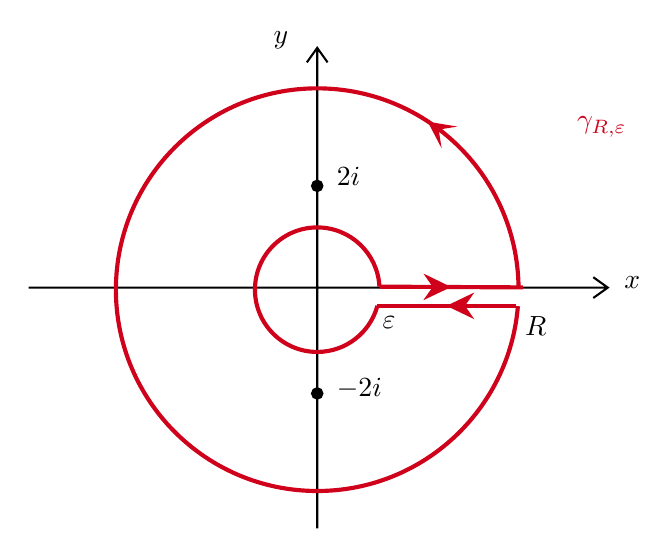
\begin{tikzpicture}[x=0.75pt,y=0.75pt,yscale=-1,xscale=1]
%uncomment if require: \path (0,253); %set diagram left start at 0, and has height of 253

%Shape: Axis 2D [id:dp4998430184566036] 
\draw  (162.5,129.13) -- (441.5,129.13)(301.5,13.63) -- (301.5,245.13) (434.5,124.13) -- (441.5,129.13) -- (434.5,134.13) (296.5,20.63) -- (301.5,13.63) -- (306.5,20.63)  ;
%Straight Lines [id:da677349311209462] 
\draw [color={rgb, 255:red, 208; green, 2; blue, 27 }  ,draw opacity=1 ][line width=1.5]    (331.47,128.68) -- (400.59,129.03) ;
\draw [shift={(366.03,128.85)}, rotate = 180.29] [fill={rgb, 255:red, 208; green, 2; blue, 27 }  ,fill opacity=1 ][line width=0.08]  [draw opacity=0] (13.4,-6.43) -- (0,0) -- (13.4,6.44) -- (8.9,0) -- cycle    ;
%Shape: Arc [id:dp05736289743124079] 
\draw  [draw opacity=0][line width=1.5]  (330.48,137.92) .. controls (327.04,150.71) and (315.37,160.13) .. (301.5,160.13) .. controls (284.93,160.13) and (271.5,146.69) .. (271.5,130.13) .. controls (271.5,113.56) and (284.93,100.13) .. (301.5,100.13) .. controls (317.58,100.13) and (330.71,112.78) .. (331.47,128.68) -- (301.5,130.13) -- cycle ; \draw  [color={rgb, 255:red, 208; green, 2; blue, 27 }  ,draw opacity=1 ][line width=1.5]  (330.48,137.92) .. controls (327.04,150.71) and (315.37,160.13) .. (301.5,160.13) .. controls (284.93,160.13) and (271.5,146.69) .. (271.5,130.13) .. controls (271.5,113.56) and (284.93,100.13) .. (301.5,100.13) .. controls (317.58,100.13) and (330.71,112.78) .. (331.47,128.68) ;
%Shape: Arc [id:dp5246954139360556] 
\draw  [draw opacity=0][line width=1.5]  (398.18,138.07) .. controls (394.14,187.93) and (352.4,227.13) .. (301.5,227.13) .. controls (247.93,227.13) and (204.5,183.7) .. (204.5,130.13) .. controls (204.5,76.55) and (247.93,33.13) .. (301.5,33.13) .. controls (354.77,33.13) and (398.01,76.06) .. (398.5,129.21) -- (301.5,130.13) -- cycle ; \draw  [color={rgb, 255:red, 208; green, 2; blue, 27 }  ,draw opacity=1 ][line width=1.5]  (398.18,138.07) .. controls (394.14,187.93) and (352.4,227.13) .. (301.5,227.13) .. controls (247.93,227.13) and (204.5,183.7) .. (204.5,130.13) .. controls (204.5,76.55) and (247.93,33.13) .. (301.5,33.13) .. controls (354.77,33.13) and (398.01,76.06) .. (398.5,129.21) ;
%Straight Lines [id:da5817066561864661] 
\draw [color={rgb, 255:red, 208; green, 2; blue, 27 }  ,draw opacity=1 ][line width=1.5]    (397.11,137.92) -- (330.48,137.92) ;
\draw [shift={(363.79,137.92)}, rotate = 360] [fill={rgb, 255:red, 208; green, 2; blue, 27 }  ,fill opacity=1 ][line width=0.08]  [draw opacity=0] (13.4,-6.43) -- (0,0) -- (13.4,6.44) -- (8.9,0) -- cycle    ;
\draw  [draw opacity=0][fill={rgb, 255:red, 208; green, 2; blue, 27 }  ,fill opacity=1 ] (361.45,62.08) -- (354.73,49.18) -- (369.08,51.55) -- (360,53) -- cycle ;
%Shape: Circle [id:dp17752216243740282] 
\draw  [color={rgb, 255:red, 0; green, 0; blue, 0 }  ,draw opacity=1 ][fill={rgb, 255:red, 0; green, 0; blue, 0 }  ,fill opacity=1 ] (299,80.13) .. controls (299,78.74) and (300.12,77.63) .. (301.5,77.63) .. controls (302.88,77.63) and (304,78.74) .. (304,80.13) .. controls (304,81.51) and (302.88,82.63) .. (301.5,82.63) .. controls (300.12,82.63) and (299,81.51) .. (299,80.13) -- cycle ;
%Shape: Circle [id:dp22166509967433679] 
\draw  [color={rgb, 255:red, 0; green, 0; blue, 0 }  ,draw opacity=1 ][fill={rgb, 255:red, 0; green, 0; blue, 0 }  ,fill opacity=1 ] (299,180.13) .. controls (299,178.74) and (300.12,177.63) .. (301.5,177.63) .. controls (302.88,177.63) and (304,178.74) .. (304,180.13) .. controls (304,181.51) and (302.88,182.63) .. (301.5,182.63) .. controls (300.12,182.63) and (299,181.51) .. (299,180.13) -- cycle ;

% Text Node
\draw (400.18,141.47) node [anchor=north west][inner sep=0.75pt]    {$R$};
% Text Node
\draw (448,122.4) node [anchor=north west][inner sep=0.75pt]    {$x$};
% Text Node
\draw (279,4.4) node [anchor=north west][inner sep=0.75pt]    {$y$};
% Text Node
\draw (331.48,141.52) node [anchor=north west][inner sep=0.75pt]    {$\varepsilon $};
% Text Node
\draw (425.18,45.47) node [anchor=north west][inner sep=0.75pt]  [color={rgb, 255:red, 208; green, 2; blue, 27 }  ,opacity=1 ]  {$\gamma _{R,\varepsilon }$};
% Text Node
\draw (309.48,69.52) node [anchor=north west][inner sep=0.75pt]    {$2i$};
% Text Node
\draw (309.48,171.52) node [anchor=north west][inner sep=0.75pt]    {$-2i$};


\end{tikzpicture}
\end{figure}
\FloatBarrier

Se prendiamo
\begin{equation*}
f( z) =\frac{\sqrt[3]{z}}{z^{2} +4}
\end{equation*}
abbiamo diversi problemi. Dobbiamo assicurarci di prendere la determinazione reale della radice.
\begin{equation*}
f(\rho ,\vartheta )=\frac{\sqrt[3]{\rho } e^{i\vartheta /3}}{\rho ^{2} e^{2i\vartheta } +4}
\end{equation*}
I poli sono in $\pm 2i$
\begin{equation*}
\begin{aligned}
\int _{\gamma _{R,\varepsilon }} f( z) dz & =2\pi i\cdotp \left(\frac{\sqrt[3]{2} e^{i\frac{\pi }{2} /3}}{4i} +\frac{\sqrt[3]{2} e^{i\frac{3\pi }{2} /3}}{-4i}\right) =\frac{\pi \sqrt[3]{2}}{2}\left( e^{i\frac{\pi }{6}} -e^{i\frac{\pi }{2}}\right)\\
\int _{\gamma _{R,\varepsilon }} f( z) dz & =\int ^{R}_{\varepsilon } +\int _{\sigma _{R}} +\int ^{\varepsilon }_{R} +\int _{\sigma _{\varepsilon }}
\end{aligned}
\end{equation*}
I due integrali sulle circonferenze tendono a $0$, con opportune maggiorazioni.

L'integrale che ci interessa è
\begin{equation*}
\int ^{R}_{\varepsilon } f( z) dz=\int ^{R}_{\varepsilon }\frac{\sqrt[3]{\rho }}{\rho ^{2} +4} d\rho \rightarrow I
\end{equation*}
L'integrale contromano va fatto facendo \textbf{attenzione} che $\vartheta =2\pi $, non più zero.
\begin{equation*}
\int ^{\varepsilon }_{R} f( z) dz=-\int ^{R}_{\varepsilon } f( z) dz=-\int ^{R}_{\varepsilon }\frac{\sqrt[3]{\rho } e^{i2\pi /3}}{\rho ^{2} +4} d\rho \rightarrow -Ie^{i2\pi /3}
\end{equation*}
Allora deduciamo che
\begin{equation*}
\begin{aligned}
\int _{\gamma _{R,\varepsilon }} & =\int ^{R}_{\varepsilon } +\int _{\sigma _{R}} +\int ^{\varepsilon }_{R} +\int _{\sigma _{\varepsilon }}\\
\frac{\pi \sqrt[3]{2}}{2}\left( e^{i\frac{\pi }{6}} -e^{i\frac{\pi }{2}}\right) & =I+0-Ie^{i2\pi /3} +0\\
 & \Rightarrow \ \ I=\frac{\frac{\pi \sqrt[3]{2}}{2}\left( e^{i\frac{\pi }{6}} -e^{i\frac{\pi }{2}}\right)}{1-e^{i2\pi /3}}
\end{aligned}
\end{equation*}
Che possiamo riscrivere
\begin{equation*}
I=\frac{\frac{\pi \sqrt[3]{2}}{2}\left(\frac{\sqrt{3}}{2} +\frac{1}{2} i-i\right)}{1-\left( -\frac{1}{2} +\frac{\sqrt{3}}{2} i\right)} =\frac{\frac{\pi \sqrt[3]{2}}{2}\left(\frac{\sqrt{3}}{2} -\frac{1}{2} i\right)}{\frac{3}{2} -\frac{\sqrt{3}}{2} i} =\frac{\frac{\pi \sqrt[3]{2}}{2}\left(\frac{\sqrt{3}}{2} -\frac{1}{2} i\right)}{\sqrt{3}\left(\frac{\sqrt{3}}{2} -\frac{1}{2} i\right)} =\frac{\pi \sqrt[3]{2}}{2\sqrt{3}}
\end{equation*}
\Soluzione

Vediamo il grafico

\fg{0.7}{07-4}

Calcoliamo il limite puntuale
\begin{equation*}
f_{n} (x)=\frac{\sqrt{n}}{1+(nx)^{2}}\xrightarrow{n\rightarrow \infty } F(x)=\begin{cases}
+\infty , & x=0\\
0, & x\neq 0
\end{cases} \ \ \Rightarrow \ \ f_{n}\xrightarrow[\text{q.o.}]{n\rightarrow \infty } 0
\end{equation*}
Controlliamo la convergenza in $L^{1}$
\begin{equation*}
\Vert f_{n} -F\Vert _{L^{1}} =\int _{\mathbb{R}}\frac{\sqrt{n}}{1+(nx)^{2}} dx=\left\{\begin{array}{ c }
nx=t\\
dx=\frac{1}{n} dt
\end{array}\right\} =\frac{1}{\sqrt{n}}\int _{\mathbb{R}}\frac{1}{1+t^{2}} dt\xrightarrow{n\rightarrow \infty } 0
\end{equation*}
Controlliamo la convergenza in $L^{p}$:
\begin{gather*}
\Vert f_{n} -F\Vert ^{p}_{L^{p}} =\int _{\mathbb{R}}\frac{n^{p/2}}{(1+(nx)^{2} )^{p}} =\left\{\begin{array}{ c }
nx=t\\
dx=\frac{1}{n} dt
\end{array}\right\} =n^{\frac{p}{2} -1}\int _{\mathbb{R}}\frac{1}{(1+t^{2} )^{p}} dt\\
\\
\Rightarrow \ \ \Vert f_{n} -F\Vert ^{p}_{L^{p}}\xrightarrow{n\rightarrow \infty } 0\ \ \Leftrightarrow \ \ \frac{p}{2} -1< 0\ \ \Leftrightarrow \ \ p< 2
\end{gather*}
Non converge in $L^{\infty }$ perché in $0$ non sono limitate.
\Soluzione

Si può vedere che con $\alpha =2$

\fg{0.6}{07-5}
\begin{equation*}
f_{n} (x)=n^{\alpha } \chi _{\left( 0;\frac{1}{n}\right)} (x)\xrightarrow[\text{q.o}]{n\rightarrow \infty } F(x)\equiv 0
\end{equation*}
Non converge in $L^{\infty }$ perché non sono limitate.

Studiamo la convergenza in $L^{p}$:
\begin{equation*}
\Vert f_{n} -F\Vert ^{p}_{L^{p}} =\int ^{1/n}_{0} n^{\alpha p} dx=n^{\alpha p-1}\rightarrow 0\ \ \Leftrightarrow \ \ \alpha p< 1\ \ \Leftrightarrow \ \ \alpha < \frac{1}{p}
\end{equation*}
\Soluzione

Vediamo il grafico

\fg{0.6}{07-6}

Limite puntuale
\begin{equation*}
\lim\limits _{n\rightarrow +\infty } f_{n}( x) =\frac{1-e^{-x}}{x} \chi _{( 0,1)} (x)=F( x)
\end{equation*}
Non abbiamo problemi di integrabilità in $0$ perché
\begin{equation*}
x\rightarrow 0,\ \ f_{n}( x) \sim \frac{x}{x} =1
\end{equation*}
Mentre in $1$
\begin{equation*}
x\rightarrow 1,\ \ f_{n}( x) \sim \frac{1-e^{-1}}{( 1-x)^{1/n}} \in L^{1}( 0,1) \ \ \Leftrightarrow \ \ n\geqslant 2
\end{equation*}
Quindi
\begin{equation*}
\Vert f_{n} -F\Vert _{L^{1}} =\int ^{1}_{0}\left| \frac{1-e^{-x}}{x( 1-x)^{1/n}} -\frac{1-e^{-x}}{x}\right| dx=\int ^{1}_{0}\frac{1-e^{-x}}{x}\left(\frac{1}{( 1-x)^{1/n}} -1\right) dx
\end{equation*}
Usiamo la convergenza dominata
\begin{equation*}
g_{n}( x) =\frac{1-e^{-x}}{x}\left(\frac{1}{( 1-x)^{1/n}} -1\right)
\end{equation*}
Prendiamo la più grande, $n=2$
\begin{equation*}
| g_{n}( x)| \leqslant g_{2}( x) \in L^{1}
\end{equation*}
Allora possiamo scambiare limite e segno dell'integrale e dedurre che c'è convergenza in $L^{1}$.
\chapter{Esercitazione 4 - Potrich}
\ParteEsercizi
\Esercizio{}

Vediamo una quarta tipologia
\begin{equation*}
\boxed{\int ^{+\infty }_{0} x^{\alpha } R\left( x^{m}\right) dx} \ \ \ \ \alpha \in \mathbb{R} ,m\in \mathbb{N} ,m\geqslant 2
\end{equation*}
Se $\alpha $ è un intero, allora si integra su curve così


\begin{figure}[htpb]
	\centering
\tikzset{every picture/.style={line width=0.75pt}} %set default line width to 0.75pt        

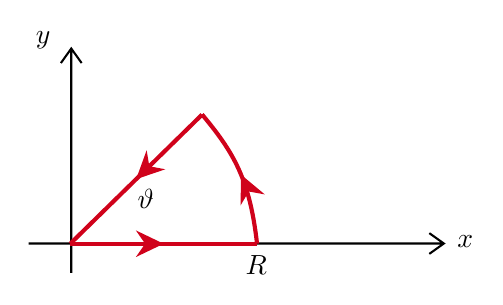
\begin{tikzpicture}[x=0.75pt,y=0.75pt,yscale=-1,xscale=1]
%uncomment if require: \path (0,137); %set diagram left start at 0, and has height of 137

%Shape: Axis 2D [id:dp5724429407600313] 
\draw  (190,109.89) -- (390,109.89)(210.5,15.95) -- (210.5,124) (383,104.89) -- (390,109.89) -- (383,114.89) (205.5,22.95) -- (210.5,15.95) -- (215.5,22.95)  ;
%Straight Lines [id:da6909710830091127] 
\draw [color={rgb, 255:red, 208; green, 2; blue, 27 }  ,draw opacity=1 ][line width=1.5]    (210,110) -- (273.5,47.8) ;
\draw [shift={(241.75,78.9)}, rotate = 315.59] [fill={rgb, 255:red, 208; green, 2; blue, 27 }  ,fill opacity=1 ][line width=0.08]  [draw opacity=0] (13.4,-6.43) -- (0,0) -- (13.4,6.44) -- (8.9,0) -- cycle    ;
%Curve Lines [id:da21980918672783578] 
\draw [color={rgb, 255:red, 208; green, 2; blue, 27 }  ,draw opacity=1 ][line width=1.5]    (273.5,47.69) .. controls (288.5,65.69) and (296.5,78.69) .. (300,110) ;
\draw [shift={(292.32,76.73)}, rotate = 65.41] [fill={rgb, 255:red, 208; green, 2; blue, 27 }  ,fill opacity=1 ][line width=0.08]  [draw opacity=0] (13.4,-6.43) -- (0,0) -- (13.4,6.44) -- (8.9,0) -- cycle    ;
%Straight Lines [id:da9818804804141448] 
\draw [color={rgb, 255:red, 208; green, 2; blue, 27 }  ,draw opacity=1 ][line width=1.5]    (210,110) -- (300,110) ;
\draw [shift={(255,110)}, rotate = 180] [fill={rgb, 255:red, 208; green, 2; blue, 27 }  ,fill opacity=1 ][line width=0.08]  [draw opacity=0] (13.4,-6.43) -- (0,0) -- (13.4,6.44) -- (8.9,0) -- cycle    ;

% Text Node
\draw (293,114.4) node [anchor=north west][inner sep=0.75pt]    {$R$};
% Text Node
\draw (395,104.4) node [anchor=north west][inner sep=0.75pt]    {$x$};
% Text Node
\draw (192,6.4) node [anchor=north west][inner sep=0.75pt]    {$y$};
% Text Node
\draw (241,82.4) node [anchor=north west][inner sep=0.75pt]    {$\vartheta $};


\end{tikzpicture}
\end{figure}
\FloatBarrier

Se $\alpha $ non è un intero, allora si integra su curve così


\begin{figure}[htpb]
	\centering
\tikzset{every picture/.style={line width=0.75pt}} %set default line width to 0.75pt        

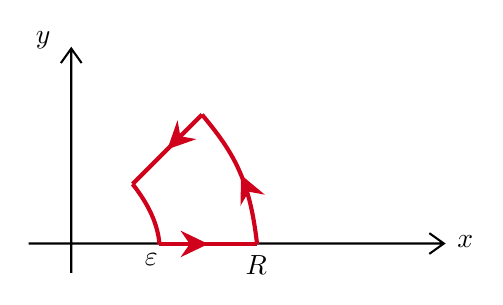
\begin{tikzpicture}[x=0.75pt,y=0.75pt,yscale=-1,xscale=1]
%uncomment if require: \path (0,137); %set diagram left start at 0, and has height of 137

%Shape: Axis 2D [id:dp029235818502451494] 
\draw  (190,109.89) -- (390,109.89)(210.5,15.95) -- (210.5,124) (383,104.89) -- (390,109.89) -- (383,114.89) (205.5,22.95) -- (210.5,15.95) -- (215.5,22.95)  ;
%Straight Lines [id:da5818987952561847] 
\draw [color={rgb, 255:red, 208; green, 2; blue, 27 }  ,draw opacity=1 ][line width=1.5]    (240.05,81.25) -- (273.5,47.8) ;
\draw [shift={(256.77,64.52)}, rotate = 315] [fill={rgb, 255:red, 208; green, 2; blue, 27 }  ,fill opacity=1 ][line width=0.08]  [draw opacity=0] (13.4,-6.43) -- (0,0) -- (13.4,6.44) -- (8.9,0) -- cycle    ;
%Curve Lines [id:da6921320122846151] 
\draw [color={rgb, 255:red, 208; green, 2; blue, 27 }  ,draw opacity=1 ][line width=1.5]    (273.5,47.8) .. controls (288.5,65.8) and (296.5,78.8) .. (300,110.11) ;
\draw [shift={(292.31,76.84)}, rotate = 65.41] [fill={rgb, 255:red, 208; green, 2; blue, 27 }  ,fill opacity=1 ][line width=0.08]  [draw opacity=0] (13.4,-6.43) -- (0,0) -- (13.4,6.44) -- (8.9,0) -- cycle    ;
%Straight Lines [id:da44850949525670036] 
\draw [color={rgb, 255:red, 208; green, 2; blue, 27 }  ,draw opacity=1 ][line width=1.5]    (253,110.11) -- (300,110.11) ;
\draw [shift={(276.5,110.11)}, rotate = 180] [fill={rgb, 255:red, 208; green, 2; blue, 27 }  ,fill opacity=1 ][line width=0.08]  [draw opacity=0] (13.4,-6.43) -- (0,0) -- (13.4,6.44) -- (8.9,0) -- cycle    ;
%Curve Lines [id:da2387592758227124] 
\draw [color={rgb, 255:red, 208; green, 2; blue, 27 }  ,draw opacity=1 ][line width=1.5]    (240.05,81.25) .. controls (245.55,88.25) and (252,98.25) .. (253,110.11) ;

% Text Node
\draw (293,114.4) node [anchor=north west][inner sep=0.75pt]    {$R$};
% Text Node
\draw (395,104.4) node [anchor=north west][inner sep=0.75pt]    {$x$};
% Text Node
\draw (192,6.4) node [anchor=north west][inner sep=0.75pt]    {$y$};
% Text Node
\draw (244.5,113.4) node [anchor=north west][inner sep=0.75pt]    {$\varepsilon $};


\end{tikzpicture}
\end{figure}
\FloatBarrier

L'ampiezza dell'angolo $\vartheta $ deve essere in entrambi i casi $\vartheta =\frac{2\pi }{m}$.



Integriamo la funzione $f( z) =e^{\alpha \log z} R\left( z^{m}\right)$.

\textbf{NB.} Se $m=2$, l'ampiezza dell'angolo sarebbe $\pi $, tuttavia il dominio del logaritmo esclude che io possa integrare lungo la semiretta $x< 0$.

Se $m=2$ allora tolgo un altro ramo.


\begin{figure}[htpb]
	\centering
\tikzset{every picture/.style={line width=0.75pt}} %set default line width to 0.75pt        

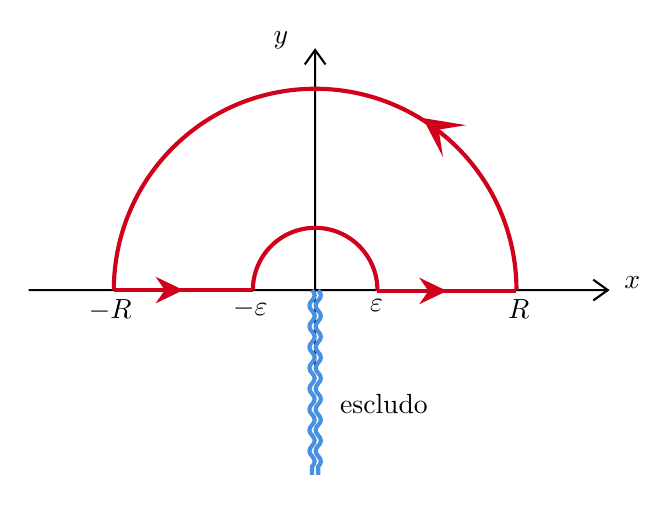
\begin{tikzpicture}[x=0.75pt,y=0.75pt,yscale=-1,xscale=1]
%uncomment if require: \path (0,238); %set diagram left start at 0, and has height of 238

%Shape: Axis 2D [id:dp48898581387364404] 
\draw  (162.5,140.33) -- (441.5,140.33)(300.5,24.63) -- (300.5,179.33) (434.5,135.33) -- (441.5,140.33) -- (434.5,145.33) (295.5,31.63) -- (300.5,24.63) -- (305.5,31.63)  ;
%Straight Lines [id:da5757902151460577] 
\draw [color={rgb, 255:red, 208; green, 2; blue, 27 }  ,draw opacity=1 ][line width=1.5]    (330.5,140.75) -- (397.5,140.75) ;
\draw [shift={(364,140.75)}, rotate = 180] [fill={rgb, 255:red, 208; green, 2; blue, 27 }  ,fill opacity=1 ][line width=0.08]  [draw opacity=0] (13.4,-6.43) -- (0,0) -- (13.4,6.44) -- (8.9,0) -- cycle    ;
%Shape: Arc [id:dp28549627239777453] 
\draw  [draw opacity=0][line width=1.5]  (270.5,140.33) .. controls (270.5,123.76) and (283.93,110.33) .. (300.5,110.33) .. controls (317.07,110.33) and (330.5,123.76) .. (330.5,140.33) .. controls (330.5,140.47) and (330.5,140.61) .. (330.5,140.75) -- (300.5,140.33) -- cycle ; \draw  [color={rgb, 255:red, 208; green, 2; blue, 27 }  ,draw opacity=1 ][line width=1.5]  (270.5,140.33) .. controls (270.5,123.76) and (283.93,110.33) .. (300.5,110.33) .. controls (317.07,110.33) and (330.5,123.76) .. (330.5,140.33) .. controls (330.5,140.47) and (330.5,140.61) .. (330.5,140.75) ;
%Shape: Arc [id:dp39883767783687163] 
\draw  [draw opacity=0][line width=1.5]  (203.5,140.33) .. controls (203.5,86.76) and (246.93,43.33) .. (300.5,43.33) .. controls (354.07,43.33) and (397.5,86.76) .. (397.5,140.33) -- (300.5,140.33) -- cycle ; \draw  [color={rgb, 255:red, 208; green, 2; blue, 27 }  ,draw opacity=1 ][line width=1.5]  (203.5,140.33) .. controls (203.5,86.76) and (246.93,43.33) .. (300.5,43.33) .. controls (354.07,43.33) and (397.5,86.76) .. (397.5,140.33) ;
%Straight Lines [id:da500527919927189] 
\draw [color={rgb, 255:red, 208; green, 2; blue, 27 }  ,draw opacity=1 ][line width=1.5]    (203.5,140.33) -- (270.5,140.33) ;
\draw [shift={(237,140.33)}, rotate = 180] [fill={rgb, 255:red, 208; green, 2; blue, 27 }  ,fill opacity=1 ][line width=0.08]  [draw opacity=0] (13.4,-6.43) -- (0,0) -- (13.4,6.44) -- (8.9,0) -- cycle    ;
\draw  [draw opacity=0][fill={rgb, 255:red, 208; green, 2; blue, 27 }  ,fill opacity=1 ] (362.12,76.27) -- (352.31,57.43) -- (373.27,60.88) -- (360,63) -- cycle ;
%Straight Lines [id:da16629969721545534] 
\draw [color={rgb, 255:red, 74; green, 144; blue, 226 }  ,draw opacity=1 ][line width=1.5]    (302,140.33) .. controls (303.67,142) and (303.67,143.66) .. (302,145.33) .. controls (300.33,147) and (300.33,148.66) .. (302,150.33) .. controls (303.67,152) and (303.67,153.66) .. (302,155.33) .. controls (300.33,157) and (300.33,158.66) .. (302,160.33) .. controls (303.67,162) and (303.67,163.66) .. (302,165.33) .. controls (300.33,167) and (300.33,168.66) .. (302,170.33) .. controls (303.67,172) and (303.67,173.66) .. (302,175.33) .. controls (300.33,177) and (300.33,178.66) .. (302,180.33) .. controls (303.67,182) and (303.67,183.66) .. (302,185.33) .. controls (300.33,187) and (300.33,188.66) .. (302,190.33) .. controls (303.67,192) and (303.67,193.66) .. (302,195.33) .. controls (300.33,197) and (300.33,198.66) .. (302,200.33) .. controls (303.67,202) and (303.67,203.66) .. (302,205.33) .. controls (300.33,207) and (300.33,208.66) .. (302,210.33) .. controls (303.67,212) and (303.67,213.66) .. (302,215.33) .. controls (300.33,217) and (300.33,218.66) .. (302,220.33) .. controls (303.67,222) and (303.67,223.66) .. (302,225.33) -- (302,229.33) -- (302,229.33)(299,140.33) .. controls (300.67,142) and (300.67,143.66) .. (299,145.33) .. controls (297.33,147) and (297.33,148.66) .. (299,150.33) .. controls (300.67,152) and (300.67,153.66) .. (299,155.33) .. controls (297.33,157) and (297.33,158.66) .. (299,160.33) .. controls (300.67,162) and (300.67,163.66) .. (299,165.33) .. controls (297.33,167) and (297.33,168.66) .. (299,170.33) .. controls (300.67,172) and (300.67,173.66) .. (299,175.33) .. controls (297.33,177) and (297.33,178.66) .. (299,180.33) .. controls (300.67,182) and (300.67,183.66) .. (299,185.33) .. controls (297.33,187) and (297.33,188.66) .. (299,190.33) .. controls (300.67,192) and (300.67,193.66) .. (299,195.33) .. controls (297.33,197) and (297.33,198.66) .. (299,200.33) .. controls (300.67,202) and (300.67,203.66) .. (299,205.33) .. controls (297.33,207) and (297.33,208.66) .. (299,210.33) .. controls (300.67,212) and (300.67,213.66) .. (299,215.33) .. controls (297.33,217) and (297.33,218.66) .. (299,220.33) .. controls (300.67,222) and (300.67,223.66) .. (299,225.33) -- (299,229.33) -- (299,229.33) ;

% Text Node
\draw (392,143.4) node [anchor=north west][inner sep=0.75pt]    {$R$};
% Text Node
\draw (448,132.4) node [anchor=north west][inner sep=0.75pt]    {$x$};
% Text Node
\draw (279,14.4) node [anchor=north west][inner sep=0.75pt]    {$y$};
% Text Node
\draw (325.5,143.4) node [anchor=north west][inner sep=0.75pt]    {$\varepsilon $};
% Text Node
\draw (190,143.4) node [anchor=north west][inner sep=0.75pt]    {$-R$};
% Text Node
\draw (259.5,143.4) node [anchor=north west][inner sep=0.75pt]    {$-\varepsilon $};
% Text Node
\draw (311,189) node [anchor=north west][inner sep=0.75pt]   [align=left] {escludo};


\end{tikzpicture}
\end{figure}
\FloatBarrier



Calcolare
\begin{equation*}
I=\int ^{+\infty }_{0}\frac{x^{\alpha }}{1+x^{3}} dx\ \ \ \ \alpha \in \mathbb{R} ,
\end{equation*}
\Esercizio{}

Vediamo una quinta tipologia
\begin{equation*}
\boxed{\begin{array}{ c l }
A & \int ^{+\infty }_{0} x^{\alpha } R( x) dx\ \ \alpha \neq 0\\
B & \int ^{+\infty }_{0} R( x) dx\\
C & \int ^{+\infty }_{0}\ln( x) R( x) dx
\end{array}}
\end{equation*}
Bisogna integrare su


\begin{figure}[htpb]
	\centering
\tikzset{every picture/.style={line width=0.75pt}} %set default line width to 0.75pt        

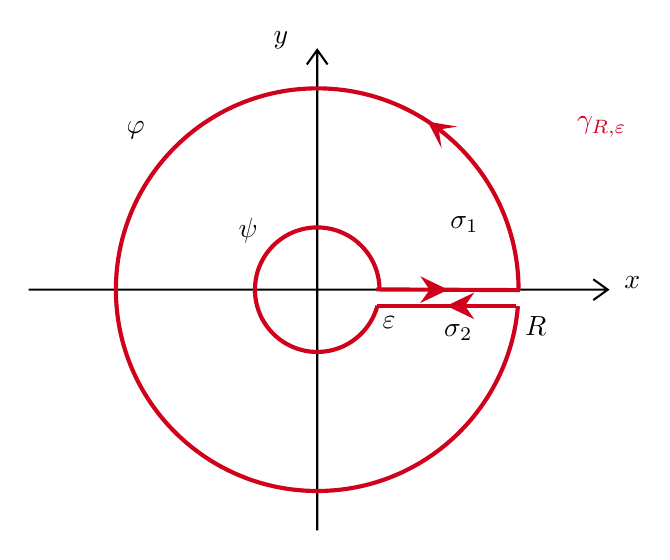
\begin{tikzpicture}[x=0.75pt,y=0.75pt,yscale=-1,xscale=1]
%uncomment if require: \path (0,253); %set diagram left start at 0, and has height of 253

%Shape: Axis 2D [id:dp376145381719732] 
\draw  (162.5,130.13) -- (441.5,130.13)(301.5,14.63) -- (301.5,246.13) (434.5,125.13) -- (441.5,130.13) -- (434.5,135.13) (296.5,21.63) -- (301.5,14.63) -- (306.5,21.63)  ;
%Straight Lines [id:da6906588690572244] 
\draw [color={rgb, 255:red, 208; green, 2; blue, 27 }  ,draw opacity=1 ][line width=1.5]    (330,130) -- (399.13,130.35) ;
\draw [shift={(364.56,130.18)}, rotate = 180.29] [fill={rgb, 255:red, 208; green, 2; blue, 27 }  ,fill opacity=1 ][line width=0.08]  [draw opacity=0] (13.4,-6.43) -- (0,0) -- (13.4,6.44) -- (8.9,0) -- cycle    ;
%Shape: Arc [id:dp11422143025607046] 
\draw  [draw opacity=0][line width=1.5]  (330.48,137.92) .. controls (327.04,150.71) and (315.37,160.13) .. (301.5,160.13) .. controls (284.93,160.13) and (271.5,146.69) .. (271.5,130.13) .. controls (271.5,113.56) and (284.93,100.13) .. (301.5,100.13) .. controls (317.99,100.13) and (331.37,113.43) .. (331.5,129.88) -- (301.5,130.13) -- cycle ; \draw  [color={rgb, 255:red, 208; green, 2; blue, 27 }  ,draw opacity=1 ][line width=1.5]  (330.48,137.92) .. controls (327.04,150.71) and (315.37,160.13) .. (301.5,160.13) .. controls (284.93,160.13) and (271.5,146.69) .. (271.5,130.13) .. controls (271.5,113.56) and (284.93,100.13) .. (301.5,100.13) .. controls (317.99,100.13) and (331.37,113.43) .. (331.5,129.88) ;
%Shape: Arc [id:dp7692032349738063] 
\draw  [draw opacity=0][line width=1.5]  (398.18,138.07) .. controls (394.14,187.93) and (352.4,227.13) .. (301.5,227.13) .. controls (247.93,227.13) and (204.5,183.7) .. (204.5,130.13) .. controls (204.5,76.55) and (247.93,33.13) .. (301.5,33.13) .. controls (355.07,33.13) and (398.5,76.55) .. (398.5,130.13) .. controls (398.5,130.16) and (398.5,130.2) .. (398.5,130.24) -- (301.5,130.13) -- cycle ; \draw  [color={rgb, 255:red, 208; green, 2; blue, 27 }  ,draw opacity=1 ][line width=1.5]  (398.18,138.07) .. controls (394.14,187.93) and (352.4,227.13) .. (301.5,227.13) .. controls (247.93,227.13) and (204.5,183.7) .. (204.5,130.13) .. controls (204.5,76.55) and (247.93,33.13) .. (301.5,33.13) .. controls (355.07,33.13) and (398.5,76.55) .. (398.5,130.13) .. controls (398.5,130.16) and (398.5,130.2) .. (398.5,130.24) ;
%Straight Lines [id:da4247309814315583] 
\draw [color={rgb, 255:red, 208; green, 2; blue, 27 }  ,draw opacity=1 ][line width=1.5]    (397.11,137.92) -- (330.48,137.92) ;
\draw [shift={(363.79,137.92)}, rotate = 360] [fill={rgb, 255:red, 208; green, 2; blue, 27 }  ,fill opacity=1 ][line width=0.08]  [draw opacity=0] (13.4,-6.43) -- (0,0) -- (13.4,6.44) -- (8.9,0) -- cycle    ;
\draw  [draw opacity=0][fill={rgb, 255:red, 208; green, 2; blue, 27 }  ,fill opacity=1 ] (361.45,62.08) -- (354.73,49.18) -- (369.08,51.55) -- (360,53) -- cycle ;

% Text Node
\draw (400.18,141.47) node [anchor=north west][inner sep=0.75pt]    {$R$};
% Text Node
\draw (448,122.4) node [anchor=north west][inner sep=0.75pt]    {$x$};
% Text Node
\draw (279,4.4) node [anchor=north west][inner sep=0.75pt]    {$y$};
% Text Node
\draw (331.48,141.52) node [anchor=north west][inner sep=0.75pt]    {$\varepsilon $};
% Text Node
\draw (208.18,47.47) node [anchor=north west][inner sep=0.75pt]    {$\varphi $};
% Text Node
\draw (262.18,94.47) node [anchor=north west][inner sep=0.75pt]    {$\psi $};
% Text Node
\draw (364.18,93.47) node [anchor=north west][inner sep=0.75pt]    {$\sigma _{1}$};
% Text Node
\draw (361.18,145.47) node [anchor=north west][inner sep=0.75pt]    {$\sigma _{2}$};
% Text Node
\draw (425.18,45.47) node [anchor=north west][inner sep=0.75pt]  [color={rgb, 255:red, 208; green, 2; blue, 27 }  ,opacity=1 ]  {$\gamma _{R,\varepsilon }$};


\end{tikzpicture}
\end{figure}
\FloatBarrier

Si interpreta $\int _{\gamma _{R,\varepsilon }} =\lim\limits _{\alpha \rightarrow 0^{+}}\int _{\Gamma _{\varepsilon ,R,\alpha }}$ dove $\Gamma _{\varepsilon ,R,\alpha }$ è


\begin{figure}[htpb]
	\centering
\tikzset{every picture/.style={line width=0.75pt}} %set default line width to 0.75pt        

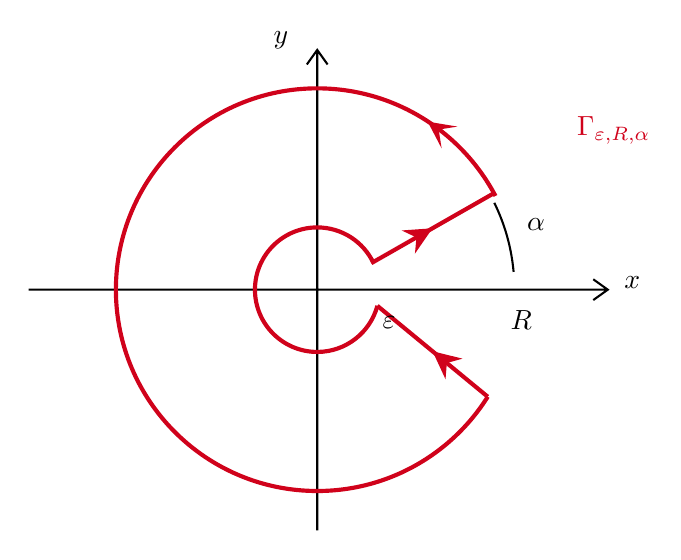
\begin{tikzpicture}[x=0.75pt,y=0.75pt,yscale=-1,xscale=1]
%uncomment if require: \path (0,253); %set diagram left start at 0, and has height of 253

%Shape: Axis 2D [id:dp4977301214304819] 
\draw  (162.5,130.13) -- (441.5,130.13)(301.5,14.63) -- (301.5,246.13) (434.5,125.13) -- (441.5,130.13) -- (434.5,135.13) (296.5,21.63) -- (301.5,14.63) -- (306.5,21.63)  ;
%Straight Lines [id:da9935131902630598] 
\draw [color={rgb, 255:red, 208; green, 2; blue, 27 }  ,draw opacity=1 ][line width=1.5]    (327.56,117.36) -- (386.5,83.73) ;
\draw [shift={(357.03,100.55)}, rotate = 510.29] [fill={rgb, 255:red, 208; green, 2; blue, 27 }  ,fill opacity=1 ][line width=0.08]  [draw opacity=0] (13.4,-6.43) -- (0,0) -- (13.4,6.44) -- (8.9,0) -- cycle    ;
%Shape: Arc [id:dp13640780925563867] 
\draw  [draw opacity=0][line width=1.5]  (330.48,137.92) .. controls (327.04,150.71) and (315.37,160.13) .. (301.5,160.13) .. controls (284.93,160.13) and (271.5,146.69) .. (271.5,130.13) .. controls (271.5,113.56) and (284.93,100.13) .. (301.5,100.13) .. controls (313.42,100.13) and (323.72,107.08) .. (328.56,117.16) -- (301.5,130.13) -- cycle ; \draw  [color={rgb, 255:red, 208; green, 2; blue, 27 }  ,draw opacity=1 ][line width=1.5]  (330.48,137.92) .. controls (327.04,150.71) and (315.37,160.13) .. (301.5,160.13) .. controls (284.93,160.13) and (271.5,146.69) .. (271.5,130.13) .. controls (271.5,113.56) and (284.93,100.13) .. (301.5,100.13) .. controls (313.42,100.13) and (323.72,107.08) .. (328.56,117.16) ;
%Shape: Arc [id:dp11391386463291964] 
\draw  [draw opacity=0][line width=1.5]  (383.66,181.71) .. controls (366.5,208.99) and (336.12,227.13) .. (301.5,227.13) .. controls (247.93,227.13) and (204.5,183.7) .. (204.5,130.13) .. controls (204.5,76.55) and (247.93,33.13) .. (301.5,33.13) .. controls (338.77,33.13) and (371.13,54.15) .. (387.38,84.98) -- (301.5,130.13) -- cycle ; \draw  [color={rgb, 255:red, 208; green, 2; blue, 27 }  ,draw opacity=1 ][line width=1.5]  (383.66,181.71) .. controls (366.5,208.99) and (336.12,227.13) .. (301.5,227.13) .. controls (247.93,227.13) and (204.5,183.7) .. (204.5,130.13) .. controls (204.5,76.55) and (247.93,33.13) .. (301.5,33.13) .. controls (338.77,33.13) and (371.13,54.15) .. (387.38,84.98) ;
%Straight Lines [id:da9801209891079499] 
\draw [color={rgb, 255:red, 208; green, 2; blue, 27 }  ,draw opacity=1 ][line width=1.5]    (383.66,181.71) -- (330.48,137.92) ;
\draw [shift={(357.07,159.81)}, rotate = 399.46000000000004] [fill={rgb, 255:red, 208; green, 2; blue, 27 }  ,fill opacity=1 ][line width=0.08]  [draw opacity=0] (13.4,-6.43) -- (0,0) -- (13.4,6.44) -- (8.9,0) -- cycle    ;
\draw  [draw opacity=0][fill={rgb, 255:red, 208; green, 2; blue, 27 }  ,fill opacity=1 ] (361.45,62.08) -- (354.73,49.18) -- (369.08,51.55) -- (360,53) -- cycle ;
%Shape: Arc [id:dp2448048568760779] 
\draw  [draw opacity=0][line width=0.75]  (386.82,88.29) .. controls (391.83,98.49) and (395.06,109.72) .. (396.12,121.58) -- (301.5,130.13) -- cycle ; \draw  [color={rgb, 255:red, 0; green, 0; blue, 0 }  ,draw opacity=1 ][line width=0.75]  (386.82,88.29) .. controls (391.83,98.49) and (395.06,109.72) .. (396.12,121.58) ;

% Text Node
\draw (393.18,138.47) node [anchor=north west][inner sep=0.75pt]    {$R$};
% Text Node
\draw (448,122.4) node [anchor=north west][inner sep=0.75pt]    {$x$};
% Text Node
\draw (279,4.4) node [anchor=north west][inner sep=0.75pt]    {$y$};
% Text Node
\draw (331.48,141.52) node [anchor=north west][inner sep=0.75pt]    {$\varepsilon $};
% Text Node
\draw (425.18,45.47) node [anchor=north west][inner sep=0.75pt]  [color={rgb, 255:red, 208; green, 2; blue, 27 }  ,opacity=1 ]  {$\Gamma _{\varepsilon ,R,\alpha }$};
% Text Node
\draw (401.18,94.47) node [anchor=north west][inner sep=0.75pt]    {$\alpha $};


\end{tikzpicture}
\end{figure}
\FloatBarrier

Dobbiamo usare la determinazione del logaritmo che esclude l'asse reale positivo
\begin{equation*}
\mathrm{Log}_{\left( 2\pi \right)} :=\ln z+i\vartheta \ \ \ \ \vartheta \in \arg z\cap \left( 0,2\pi \right)
\end{equation*}
Si considera rispettivamente
\begin{equation*}
\begin{array}{ c l }
A & f\left( z\right) =e^{\alpha \cdotp \mathrm{Log}_{\left( 2\pi \right)} z} R\left( z\right)\\
B & f\left( z\right) =\mathrm{Log}_{\left( 2\pi \right)} z\cdotp R\left( z\right)\\
C & f\left( z\right) =\left(\mathrm{Log}_{\left( 2\pi \right)} z\right)^{2} R\left( z\right)
\end{array}
\end{equation*}


Calcolare


\begin{equation*}
I=\int ^{+\infty }_{0}\frac{1}{\sqrt{x}\left( 1+x\right)} dx=\int ^{+\infty }_{0}\frac{x^{-1/2}}{\left( 1+x\right)} dx
\end{equation*}
\Esercizio{}

Calcolare
\begin{equation*}
I=\int ^{+\infty }_{0}\frac{1}{\left( x^{2} +4\right)\left( x+1\right)} dx
\end{equation*}
\Esercizio{(Spazi $L^{p}$)}

Si considerino le seguenti funzioni definite su $\left( 0,+\infty \right)$ nel seguente modo
\begin{equation*}
f\left( x\right) =\frac{1}{\sqrt{x}} \ \ \ \ g\left( x\right) =\frac{1}{\sqrt{x+1}}
\end{equation*}
\begin{enumerate}
\item Stabilire per quali $p\in \left[ 1,+\infty \right]$ le seguenti funzioni stanno in $L^{p}\left( 1,+\infty \right)$:\begin{equation*}
f\ \ \ \ g\ \ \ \ f-g\ \ \ \ \frac{g}{f}
\end{equation*}
\item Stessa domanda in $\left( 0,1\right)$
\end{enumerate}
\Esercizio{ }

Sia $B=\left\{\left( x,y\right) \in \mathbb{R}^{2} :x^{2} +y^{2} \leqslant 1\right\}$ e sia
\begin{equation*}
f\left( x,y\right) =\frac{1}{\sqrt{x^{2} +y^{2}}}
\end{equation*}
\begin{enumerate}
\item Stabilire per quali $p\geqslant 1$ si ha $f\in L^{p}\left( B\right)$
\item Stabilire per quali $q$ si ha $f\in L^{q}\left(\mathbb{R}^{2} \setminus B\right)$.
\end{enumerate}
\Esercizio{}

Sia
\begin{equation*}
f_{n}\left( x\right) =\frac{n^{2}\sin\left(\frac{x^{2}}{n^{2}}\right)}{\left( x^{2} +n^{2}\right)^{3/2}\log^{3/2}\left( x^{2} +n^{2}\right)} \ \ n\in \mathbb{N}
\end{equation*}
Rispondere ai seguenti quesiti
\begin{enumerate}
\item Per quali $n\in \mathbb{N}$ si ha $f_{n} \in L^{1}\left( 0,+\infty \right)$.
\item Determinare la funzione limite $f$ in $\left( 0,+\infty \right)$.
\item Calcolare $\lim\limits _{n\rightarrow +\infty }\int ^{+\infty }_{0} f_{n}\left( x\right) dx$
\end{enumerate}
\Esercizio{}

Date le $f_{n}\left( x\right) =\arctan\left( nx\right)$ definite su $\left[ 0,+\infty \right)$. 
\begin{enumerate}
\item Determinare il limite puntuale $f\left( x\right)$
\item Stabilire se $f_{n}\rightarrow f$ in $L^{p}\left( 0,+\infty \right)$ per $p\in \left[ 1,+\infty \right)$.
\end{enumerate}
\ParteSoluzioni
\Soluzione

$f_{\alpha } \sim x^{\alpha -3} \ \ x\rightarrow +\infty $.

$f_{\alpha }$ è integrabile in un intorno di $+\infty $ se e solo se $3-\alpha  >1$, cioè $\Leftrightarrow \alpha < 2$.

$f_{\alpha } \sim x^{\alpha } \ \ x\rightarrow 0^{+}$.

$f_{\alpha }$ è integrabile in senso proprio in un intorno destro di $0$ $\Leftrightarrow -\alpha < 1\Leftrightarrow \alpha  >-1$.

$\Rightarrow \exists I$ se e solo se $-1< \alpha < 2$.



Sia $f\left( z\right) =\frac{e^{\alpha \log z}}{1+z^{3}}$.

Considero un angolo $=\frac{2\pi }{m} =\frac{2\pi }{3}$


\begin{figure}[htpb]
	\centering
\tikzset{every picture/.style={line width=0.75pt}} %set default line width to 0.75pt        

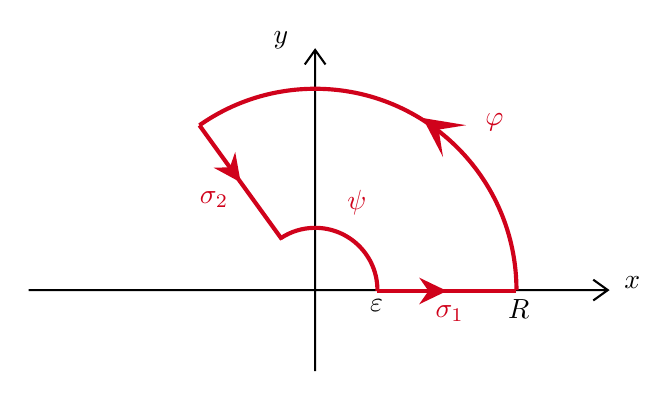
\begin{tikzpicture}[x=0.75pt,y=0.75pt,yscale=-1,xscale=1]
%uncomment if require: \path (0,193); %set diagram left start at 0, and has height of 193

%Shape: Axis 2D [id:dp38802361743556224] 
\draw  (162.5,140.33) -- (441.5,140.33)(300.5,24.63) -- (300.5,179.33) (434.5,135.33) -- (441.5,140.33) -- (434.5,145.33) (295.5,31.63) -- (300.5,24.63) -- (305.5,31.63)  ;
%Straight Lines [id:da7713867715877043] 
\draw [color={rgb, 255:red, 208; green, 2; blue, 27 }  ,draw opacity=1 ][line width=1.5]    (330.5,140.75) -- (397.5,140.75) ;
\draw [shift={(364,140.75)}, rotate = 180] [fill={rgb, 255:red, 208; green, 2; blue, 27 }  ,fill opacity=1 ][line width=0.08]  [draw opacity=0] (13.4,-6.43) -- (0,0) -- (13.4,6.44) -- (8.9,0) -- cycle    ;
%Shape: Arc [id:dp12128862418563902] 
\draw  [draw opacity=0][line width=1.5]  (283.84,115.38) .. controls (288.61,112.19) and (294.34,110.33) .. (300.5,110.33) .. controls (317.07,110.33) and (330.5,123.76) .. (330.5,140.33) .. controls (330.5,140.47) and (330.5,140.61) .. (330.5,140.75) -- (300.5,140.33) -- cycle ; \draw  [color={rgb, 255:red, 208; green, 2; blue, 27 }  ,draw opacity=1 ][line width=1.5]  (283.84,115.38) .. controls (288.61,112.19) and (294.34,110.33) .. (300.5,110.33) .. controls (317.07,110.33) and (330.5,123.76) .. (330.5,140.33) .. controls (330.5,140.47) and (330.5,140.61) .. (330.5,140.75) ;
%Shape: Arc [id:dp7213752730044614] 
\draw  [draw opacity=0][line width=1.5]  (244.75,60.94) .. controls (260.52,49.84) and (279.75,43.33) .. (300.5,43.33) .. controls (354.07,43.33) and (397.5,86.76) .. (397.5,140.33) -- (300.5,140.33) -- cycle ; \draw  [color={rgb, 255:red, 208; green, 2; blue, 27 }  ,draw opacity=1 ][line width=1.5]  (244.75,60.94) .. controls (260.52,49.84) and (279.75,43.33) .. (300.5,43.33) .. controls (354.07,43.33) and (397.5,86.76) .. (397.5,140.33) ;
%Straight Lines [id:da09050365562806317] 
\draw [color={rgb, 255:red, 208; green, 2; blue, 27 }  ,draw opacity=1 ][line width=1.5]    (244.75,60.94) -- (284.5,115.89) ;
\draw [shift={(264.62,88.42)}, rotate = 234.12] [fill={rgb, 255:red, 208; green, 2; blue, 27 }  ,fill opacity=1 ][line width=0.08]  [draw opacity=0] (13.4,-6.43) -- (0,0) -- (13.4,6.44) -- (8.9,0) -- cycle    ;
\draw  [draw opacity=0][fill={rgb, 255:red, 208; green, 2; blue, 27 }  ,fill opacity=1 ] (362.12,76.27) -- (352.31,57.43) -- (373.27,60.88) -- (360,63) -- cycle ;

% Text Node
\draw (392,143.4) node [anchor=north west][inner sep=0.75pt]    {$R$};
% Text Node
\draw (448,132.4) node [anchor=north west][inner sep=0.75pt]    {$x$};
% Text Node
\draw (279,14.4) node [anchor=north west][inner sep=0.75pt]    {$y$};
% Text Node
\draw (325.5,143.4) node [anchor=north west][inner sep=0.75pt]    {$\varepsilon $};
% Text Node
\draw (381,53.9) node [anchor=north west][inner sep=0.75pt]  [color={rgb, 255:red, 208; green, 2; blue, 27 }  ,opacity=1 ]  {$\varphi $};
% Text Node
\draw (314.5,90.9) node [anchor=north west][inner sep=0.75pt]  [color={rgb, 255:red, 208; green, 2; blue, 27 }  ,opacity=1 ]  {$\psi $};
% Text Node
\draw (243.5,91.4) node [anchor=north west][inner sep=0.75pt]  [color={rgb, 255:red, 208; green, 2; blue, 27 }  ,opacity=1 ]  {$\sigma _{2}$};
% Text Node
\draw (357,146.4) node [anchor=north west][inner sep=0.75pt]  [color={rgb, 255:red, 208; green, 2; blue, 27 }  ,opacity=1 ]  {$\sigma _{1}$};


\end{tikzpicture}
\end{figure}
\FloatBarrier

Chiamo l'intera curva $\gamma _{R,\varepsilon } =\sigma _{1} \cup \varphi \cup \sigma _{2} \cup \psi $

Per il teorema dei residui
\begin{equation*}
\int _{\gamma _{R,\varepsilon }} f\left( z\right) dz=2\pi i\cdotp \mathrm{Res}\left( f,e^{i\pi /3}\right)
\end{equation*}
$e^{i\pi /3}$ è l'unico punto interno alla curva in cui si annulla il denominatore.
\begin{equation*}
\begin{aligned}
\int _{\gamma _{R,\varepsilon }} & =\int _{\sigma _{1}} +\int _{\varphi } +\int _{\sigma _{2}} +\int _{\psi }\\
 & \\
\int _{\sigma _{1}} & =\left\{\begin{array}{ c }
z=t\\
t\in [ \varepsilon ,R]
\end{array}\right\} =\int ^{R}_{\varepsilon }\frac{e^{\alpha \ln t}}{1+t^{3}} dt\xrightarrow[R\rightarrow +\infty ]{\varepsilon \rightarrow 0^{+}} I\\
 & \\
\int _{\sigma _{2}} & =\left\{\begin{array}{ c }
z=te^{i2\pi /3}\\
t\in [ \varepsilon ,R]
\end{array}\right\} =-\int ^{R}_{\varepsilon }\frac{e^{\alpha \ln te^{i2\pi /3}}}{1+t^{3}} e^{i2\pi /3} dt=-\int ^{R}_{\varepsilon }\frac{e^{\alpha \left(\ln t+\ln e^{i2\pi /3}\right)}}{1+t^{3}} e^{i2\pi /3} dt\\
 & =-\int ^{R}_{\varepsilon }\frac{e^{\alpha (\ln t+i2\pi /3)}}{1+t^{3}} e^{i2\pi /3} dt=-e^{i\frac{2}{3} \pi ( 1+\alpha )}\int ^{R}_{\varepsilon }\frac{e^{\alpha \ln t}}{1+t^{3}} dt\\
 & \xrightarrow[R\rightarrow +\infty ]{\varepsilon \rightarrow 0^{+}} -e^{i\frac{2}{3} \pi ( 1+\alpha )} I\\
 & \\
\left| \int _{\varphi }\right|  & =\left\{\begin{array}{ c }
z=Re^{it}\\
t\in [ 0,2\pi /3]
\end{array}\right\} =\left| \int ^{2\pi /3}_{0}\frac{e^{\alpha (\ln R+it)}}{1+R^{3} e^{i3t}}\textcolor[rgb]{0.29,0.56,0.89}{\underbrace{Rie^{it}}_{\gamma '}} dt\right| =\int ^{2\pi /3}_{0}\frac{\left| e^{\alpha (\ln R+it)}\right| }{\left| 1+R^{3} e^{i3t}\right| }\textcolor[rgb]{0.82,0.01,0.11}{\left| Rie^{it}\right| } dt\\
 & \textcolor[rgb]{0.96,0.65,0.14}{| | a| -| b| | \leqslant | a+b| \leqslant | a| +| b| }\\
 & \leqslant \int ^{2\pi /3}_{0}\frac{\left| e^{\alpha (\ln R+it)}\right| }{\left| 1-R^{3}\right| }\textcolor[rgb]{0.82,0.01,0.11}{R} dt\leqslant \frac{R^{\alpha +1}}{\left| 1-R^{3}\right| }\frac{2\pi }{3} dt\sim \frac{2\pi }{3}\frac{1}{R^{2-\alpha }}\xrightarrow[\alpha \in ( -1,2)]{R\rightarrow +\infty } 0\\
 & \\
\left| \int _{\psi }\right|  & =\left\{\begin{array}{ c }
z=\varepsilon e^{it}\\
t\in [ 0,2\pi /3]
\end{array}\right\} =\left| \int ^{2\pi /3}_{0}\frac{e^{\alpha (\ln \varepsilon +it)}}{1+\varepsilon ^{3} e^{i3t}}\textcolor[rgb]{0.29,0.56,0.89}{\underbrace{\varepsilon ie^{it}}_{\gamma '}} dt\right| \leqslant \dotsc \leqslant \frac{2\pi }{3} \varepsilon ^{\alpha +1}\xrightarrow[\alpha \in ( -1,2)]{\varepsilon \rightarrow 0^{+}} 0\\
 & \\
\Rightarrow  & \ \ \frac{2\pi i\cdotp \mathrm{Res}\left( f,e^{i\pi /3}\right)}{1-e^{i\frac{2}{3} \pi ( 1+\alpha )}} =I
\end{aligned}
\end{equation*}
Resta solo da calcolare il residuo.
\Soluzione

Devo considerare la forma $A$
\begin{gather*}
f( z) =e^{-\frac{1}{2}\mathrm{Log}_{( 2\pi )} z} \cdotp \frac{1}{1+z}\\
\int _{\gamma _{\varepsilon ,R}} f( z) dz=2\pi i\cdotp \sum \mathrm{Res}( f) =2\pi i\cdotp \mathrm{Res}( f,-1)
\end{gather*}
Ugualmente
\begin{equation*}
\begin{aligned}
\int _{\gamma _{R,\varepsilon }} & =\int _{\sigma _{1}} +\int _{\varphi } +\int _{\sigma _{2}} +\int _{\psi }\\
 & \\
\int _{\sigma _{1} \cup \sigma _{2}} & =\left\{\begin{array}{ c }
z=t\\
t\in [ \varepsilon ,R]
\end{array}\right\} =\int ^{R}_{\varepsilon }\frac{1}{1+t}\left[ e^{-\frac{1}{2}\ln t} -e^{-\frac{1}{2}(\ln t+2\pi i)}\right] dt\\
 & =\underbrace{\left( 1-e^{-\pi i}\right)}_{1+1=2}\int ^{R}_{\varepsilon }\frac{1}{\sqrt{t}( 1+t)} dt\xrightarrow[R\rightarrow +\infty ]{\varepsilon \rightarrow 0^{+}} 2I\\
 & \\
\int _{\varphi } & \xrightarrow{R\rightarrow +\infty } 0\\
\int _{\psi } & \xrightarrow{\varepsilon \rightarrow 0^{+}} 0\\
 & \\
\Rightarrow  & \ \ 2I=2\pi i\cdotp \mathrm{Res}( f,-1) \ \ \Rightarrow \ \ I=\pi i\cdotp \mathrm{Res}( f,-1)
\end{aligned}
\end{equation*}
\Soluzione

Siamo nel caso $B$
\begin{gather*}
f\left( z\right) =\mathrm{Log}_{\left( 2\pi \right)} z\cdotp R\left( z\right) =f\left( z\right) =\frac{\mathrm{Log}_{\left( 2\pi \right)} z}{\left( z^{2} +4\right)\left( z+1\right)}\\
\int _{\gamma _{\varepsilon ,R}} f\left( z\right) dz=2\pi i\cdotp \sum \mathrm{Res}\left( f,z_{i}\right)
\end{gather*}
Il denominatore si annulla per $z=-1,\pm 2i$.
\begin{equation*}
\begin{aligned}
\int _{\gamma _{R,\varepsilon }} & =\int _{\sigma _{1}} +\int _{\varphi } +\int _{\sigma _{2}} +\int _{\psi }\\
 & \\
\int _{\sigma _{1} \cup \sigma _{2}} & =\left\{\begin{array}{ c }
z=t\\
t\in \left[ \varepsilon ,R\right]
\end{array}\right\} =\int ^{R}_{\varepsilon }\frac{1}{\left( t+1\right)\left( t^{2} +4\right)}\left[\ln t-\left(\ln t+2\pi i\right)\right] dt\xrightarrow[R\rightarrow +\infty ]{\varepsilon \rightarrow 0^{+}} -2\pi iI\\
 & \\
\int _{\varphi } & \xrightarrow{R\rightarrow +\infty } 0\\
\int _{\psi } & \xrightarrow{\varepsilon \rightarrow 0^{+}} 0
\end{aligned}
\end{equation*}
\Soluzione

Rispondiamo al punto $1$.
\begin{equation*}
\ \begin{aligned}
\left| f\left( x\right)\right| ^{p} & =\frac{1}{x^{p/2}} \ \ \Rightarrow \ \ f\in L^{p}\left( 1,+\infty \right) \ \ \Leftrightarrow \ \ \frac{p}{2}  >1\ \ \Leftrightarrow \ \ p >2\ \left( +\infty \ \text{incluso}\right)\\
 & \\
\left| g\left( x\right)\right| ^{p} & =\frac{1}{\left( x+1\right)^{p/2}}\overset{x\rightarrow +\infty }{\sim }\frac{1}{x^{p/2}} \ \ \Rightarrow \ \ g\in L^{p}\left( 1,+\infty \right) \ \ \Leftrightarrow \ \ p >2\ \left( +\infty \ \text{incluso}\right)\\
 & \\
\left| f-g\right| ^{p} & =\left| \frac{1}{\sqrt{x}} -\frac{1}{\sqrt{x+1}}\right| ^{p} =\left| \frac{\sqrt{x+1} -\sqrt{x}}{\sqrt{x}\sqrt{x+1}}\right| ^{p}\\
 & =\left| \frac{\sqrt{x+1} -\sqrt{x}}{\sqrt{x^{2} +x}} \cdotp \frac{\sqrt{x+1} +\sqrt{x}}{\sqrt{x+1} +\sqrt{x}}\right| ^{p} =\left| \frac{x+1-x}{\sqrt{x^{2} +x}\left(\sqrt{x+1} +\sqrt{x}\right)}\right| ^{p}\\
 & =\left| \frac{x+1-x}{\sqrt{x^{2} +x}\left(\sqrt{x+1} +\sqrt{x}\right)}\right| ^{p}\overset{x\rightarrow +\infty }{\sim }\left| \frac{1}{x\left( 2\sqrt{x}\right)}\right| ^{p} =\frac{1}{2^{p} x^{3p/2}}\\
 & \Rightarrow \ \ f-g\in L^{p}\left( 1,+\infty \right) \ \ \Leftrightarrow \ \ \frac{3}{2} p >1\ \ \Leftrightarrow \ \ p >\frac{2}{3} \ \text{cioè il primo intero:} \ p\geqslant 1\\
 & \\
\frac{g\left( x\right)}{f\left( x\right)} & \overset{x\rightarrow +\infty }{\sim } 1\ \ \Rightarrow \ \ \frac{g}{f} \in L^{p}\left( 1,+\infty \right) \ \ \Leftrightarrow \ \ p=+\infty 
\end{aligned}
\end{equation*}
Rispondiamo al punto $2$.
\begin{equation*}
| f( x)| ^{p}\overset{x\rightarrow 0^{+}}{\sim }\frac{1}{x^{p/2}} \ \ \Rightarrow \ \ f\in L^{p}( 0,1) \ \ \Leftrightarrow \ \ \frac{p}{2} < 1\ \ \Leftrightarrow \ \ 1\leqslant p< 2
\end{equation*}
$g$ è limitata in $( 0,1) \Rightarrow g\in L^{p}( 0,1) \ \forall p\geqslant 1$, incluso $+\infty $.

$f-g\in L^{p}( 0,1) \Leftrightarrow 1\leqslant p< 2$ dato che so sommando due funzioni, di cui una limitata su intervallo limitato che non presenta problemi e una in $L^{p}$ per $1\leqslant p< 2$.

$\frac{g}{f} \in L^{p}( 0,1) \ \forall p\geqslant 1$, incluso $+\infty $.
\Soluzione

Rispondiamo al punto $1$.

Passiamo in coordinate polari centrate nell'origine
\begin{gather*}
\begin{cases}
x=\rho \cos \vartheta \\
y=\rho \sin \vartheta 
\end{cases} \ \ \Rightarrow \ \ \iint _{B}| f( x,y)| ^{p} dxdy=\iint _{B^{\star }}\left| \frac{1}{\rho }\right| ^{p} \rho d\rho d\vartheta \\
\\
B^{\star } =\{( \rho ,\vartheta ) :0\leqslant \rho \leqslant 1,0< \vartheta < 2\pi \}\\
\\
\int ^{2\pi }_{0} d\vartheta \int ^{1}_{0}\frac{1}{\rho ^{p-1}} d\rho < +\infty \ \ \Leftrightarrow \ \ p-1< 1\ \ \Leftrightarrow \ \ p< 2\land p\geqslant 1
\end{gather*}
Rispondiamo al punto $2$.
\begin{gather*}
\iint _{\mathbb{R}^{2} \setminus B}| f( x,y)| ^{q} dxdy=2\pi \int ^{+\infty }_{1}\frac{1}{\rho ^{q-1}} d\rho < +\infty \ \ \Leftrightarrow \ \ q-1 >1\\
\Leftrightarrow q >2\ \left( +\infty \ \text{incluso}\right)
\end{gather*}
\Soluzione
\begin{theorem}
[della convergenza dominata] Sia $\{f_{n}\}$ una successione di funzioni misurabili su un insieme $\Omega \subset \mathbb{R}^{n}$ misurabile. Supponiamo che siano verificate le seguenti due condizioni:\footnote{È importante che la $g$ non dipenda da $n$.}
\begin{equation*}
\begin{cases}
f_{n}\xrightarrow{n\rightarrow +\infty } f\ \text{q.o. in} \ \Omega \\
\exists g\in L^{1}( \Omega ) :| f_{n}| \leqslant g( x) \ \text{per q.o.} \ x\in \Omega ,\ \forall n\in \mathbb{N}
\end{cases}
\end{equation*}
Allora
\begin{equation*}
f\in L^{1}( \Omega ) ,\ \ \ \ \lim _{n\rightarrow +\infty }\int _{\Omega } f_{n}( x) dx=\int _{\Omega }\lim _{n\rightarrow +\infty } f_{n}( x) dx
\end{equation*}
\end{theorem}
\begin{enumerate}
\item Le $f_{n}$ sono continue su $E=( 0,+\infty )$ e quindi misurabili su $E$

$\forall n >0$ fissato si ha\begin{equation*}
| f_{n}( x)| \leqslant \frac{n^{2}}{\left( x^{2}\right)^{3/2}\log^{3/2}\left( x^{2}\right)} =\frac{n^{2}}{x^{3}( 2\log x)^{3/2}} =\frac{n^{2}}{2^{3/2} x^{3}(\log x)^{3/2}} \ \ x\rightarrow +\infty 
\end{equation*}

$f_{n}$ è integrabile nell'intorno di $+\infty ,\forall n >0$.\begin{equation*}
\text{per} \ x\rightarrow 0\ \ f( x) \sim \begin{cases}
\frac{x^{2}}{n^{3}\log^{3/2}\left( n^{2}\right)} , & n\geqslant 2\\
\frac{x^{2}}{\log^{3/2}\left( x^{2} +1\right)} \sim \frac{x^{2}}{x^{3}} =\frac{1}{x} , & n=1
\end{cases}
\end{equation*}

$f_{n}$ sono integrabili in $U\left( 0^{+}\right) ,\forall n\geqslant 2$.

$\Rightarrow f_{n} \in L^{1}( 0,+\infty ) \Leftrightarrow n\geqslant 2$.
\item Calcoliamo\begin{equation*}
\begin{aligned}
\lim _{n\rightarrow +\infty } f_{n}( x_{0}) & =\left\{x_{0} \ \text{è fissato}\right\}\\
 & =\lim _{n\rightarrow +\infty }\frac{n^{2}\sin\left(\frac{x^{2}_{0}}{n^{2}}\right)}{\left( x^{2}_{0} +n^{2}\right)^{3/2}\log^{3/2}\left( x^{2}_{0} +n^{2}\right)}\\
 & =\lim _{n\rightarrow +\infty }\frac{x^{2}_{0}}{n^{3}\log^{3/2}\left( n^{2}\right)} =0
\end{aligned}
\end{equation*}

$f_{n}$ converge puntualmente alla funzione limite $f( x) \equiv 0$.
\item Osservo\begin{equation*}
| \sin x| \leqslant x\ \ \forall x\in ( 0,+\infty ) \ \ \Rightarrow \ \ n^{2}\sin\left(\frac{x^{2}}{n^{2}}\right) \leqslant n^{2}\frac{x^{2}}{n^{2}} =x^{2}
\end{equation*}

Per $n\geqslant 2$\begin{equation*}
| f_{n}( x)| \leqslant g( x) :=\frac{x^{2}}{\left( x^{2} +2^{2}\right)^{3/2}\log^{3/2}\left( x^{2} +2^{2}\right)} \in L^{1}( 0,+\infty )
\end{equation*}
\begin{enumerate}
\item diminuisco il denominatore
\item devo ottenere qualcosa che \underline{\textbf{non dipende}} da $n$
\end{enumerate}

$\overset{\text{Dom}}{\Rightarrow }\lim\limits _{n\rightarrow +\infty }\int ^{+\infty }_{0} f_{n}( x) dx=\int ^{+\infty }_{0}\lim\limits _{n\rightarrow +\infty } f_{n}( x) dx=0$.
\end{enumerate}
\Soluzione
\begin{definition}
\begin{equation*}
f_{n}\xrightarrow[n\rightarrow +\infty ]{L^{p}} f\ ( p\in [ 1,+\infty )) \ \ \Leftrightarrow \ \ \Vert f_{n} -f\Vert ^{p}_{L^{p}}\xrightarrow{n\rightarrow +\infty } 0
\end{equation*}
\end{definition}
\begin{enumerate}
\item Fisso $x_{0} \in [ 0,+\infty )$
\begin{enumerate}
\item se $x_{0} =0\ \ \Rightarrow \ \ f_{n}( 0) =0$
\item se $x_{0} \neq 0\ \ \Rightarrow \ \ \lim\limits _{n\rightarrow +\infty } f_{n}( x) =\frac{\pi }{2}$
\end{enumerate}

$\Rightarrow \ \ \{f_{n}\}_{n\in \mathbb{N}}$ converge puntualmente a $f( x) =\begin{cases}
0, & x=0\\
\pi /2, & x\neq 0
\end{cases}$

\fg{0.7}{08-7}
\item Se $x >0$\begin{gather*}
f( x) -f_{n}( x) =\frac{\pi }{2} -\arctan( nx) =\arctan\left(\frac{1}{nx}\right)\\
\Rightarrow \ \ \Vert f_{n} -f\Vert ^{p}_{L^{p}} =\int ^{+\infty }_{0}\left(\arctan\left(\frac{1}{nx}\right)\right)^{p} dx
\end{gather*}

Escludo $p=1$, perché $\arctan\left(\frac{1}{nx}\right) \sim \frac{1}{nx}$ e $\frac{1}{x}$ non è integrabile a $+\infty $.

Verifichiamo le ipotesi della convergenza dominata.\begin{equation*}
\left| \left(\arctan\left(\frac{1}{nx}\right)\right)^{p}\right| \leqslant g( x) :=\begin{cases}
\left(\frac{\pi }{2}\right)^{p} , & 0< x< 1\ \left(\text{integrabile in zero} \ \forall p\right)\\
\left| \frac{1}{x}\right| ^{p} & x\geqslant 1\ \left(\text{uso proprio} \ n=1\ \text{per maggiorare}\right)
\end{cases}
\end{equation*}

$\overset{\text{Dom}}{\Rightarrow }\lim\limits _{n\rightarrow +\infty }\Vert f_{n} -f\Vert ^{p}_{L^{p}} =\lim\limits _{n\rightarrow +\infty }\int ^{+\infty }_{0}\left(\arctan\left(\frac{1}{nx}\right)\right)^{p} dx=\int ^{+\infty }_{0}\lim\limits _{n\rightarrow +\infty }\left(\arctan\left(\frac{1}{nx}\right)\right)^{p} dx=0$
\end{enumerate}
\chapter{Esercitazione 5 - Boella}
\ParteEsercizi
\Esercizio{}

Studiare la convergenza di
\begin{equation*}
f( x,y) =\frac{1}{(x^{2} +y^{2} )^{\alpha }\sqrt{1+x^{2} +y^{2}}}
\end{equation*}
scegliendo $\alpha $ tale per cui:
\begin{itemize}
\item $f\in L^{1} (\mathbb{R} )$
\item $f\in L^{p} (\mathbb{R} )$
\item $f\in L^{\infty } (\mathbb{R} )$
\end{itemize}
\Esercizio{}

Studiare la convergenza (ovvero limite puntuale, limite in $L^{p}$, limite in $L^{\infty }$, della seguente serie di funzioni:
\begin{equation*}
f_{n} (x)=\pi -2\arctan (|x|^{n} )
\end{equation*}
\Esercizio{}

Analizzare la seguente serie:
\begin{equation*}
f(x)=\sum ^{\infty }_{n=1}\frac{n+1}{n^{4} +n}\sin (n\pi x)
\end{equation*}
\begin{itemize}
\item $f_{n} (x)\in L^{2}$?
\item Che periodo ha?
\item Si può dire qualcosa anche sulla continuità?
\end{itemize}
\Esercizio{}

Data una funzione $2\pi $-periodica
\begin{equation*}
f:[ 0,2\pi )\rightarrow \mathbb{R} \ \ \ \ f(x)=x
\end{equation*}
Determinare la sue serie di Fourier. Si riesce a ricondurre la serie ad una nota?
\Esercizio{}

Data una funzione $1$-periodica dispari
\begin{equation*}
f:[ 0,1]\rightarrow \mathbb{R} \ \ \ \ f(x)=x-x^{2}
\end{equation*}
Determinare la sue serie di Fourier.
\ParteSoluzioni
\Soluzione

Sicuramente non appartiene a $L^{\infty }$ a meno che $\alpha $ non sia negativo dato che se $\alpha $ è positivo questa funzione ha un asintoto verticale.

Per vedere se $f\in L^{1}$, posto che sia sempre positiva, basta integrarla su tutto il piano e passare in coordinate polari. Quindi dovrà convergere l'integrale doppio
\begin{gather*}
\int ^{2\pi }_{0} d\vartheta \int ^{+\infty }_{0}\underbrace{\frac{1}{\rho ^{2}\sqrt{1+\rho ^{2}}} \rho }_{g( \rho )} d\rho \\
\begin{aligned}
\rho \rightarrow 0, & \ \ g(\rho )\sim \frac{1}{\rho ^{2\alpha -1}} \ \ \Rightarrow \ \ 2\alpha -1< 1\ \ \Rightarrow \ \ \alpha < 1\\
\rho \rightarrow +\infty , & \ \ g(\rho )\sim \frac{1}{\rho ^{2\alpha }} \ \ \Rightarrow \ \ 2\alpha  >1\ \ \Rightarrow \ \ \alpha  >\frac{1}{2}
\end{aligned}
\end{gather*}
Quindi
\begin{equation*}
f(x,y)\in L^{1} (\mathbb{R}^{2} )\ \ \Leftrightarrow \ \ \frac{1}{2} < \alpha < 1
\end{equation*}
Se invece consideriamo il generico $L^{p}$ dobbiamo elevare alla $p$, ma non il $\rho $ dello Jacobiano
\begin{equation*}
g(\rho )=\frac{\rho }{\rho ^{2\alpha p}\left(\sqrt{1+\rho ^{2}}\right)^{p}}
\end{equation*}
Calcoliamo
\begin{equation*}
\begin{aligned}
\rho \rightarrow 0^{+} , & \ \ g(\rho )\sim \frac{1}{\rho ^{2\alpha p-1}} \ \ \Rightarrow \ \ 2\alpha p-1< 1\ \ \Rightarrow \ \ \alpha < \frac{1}{\rho }\\
\rho \rightarrow +\infty , & \ \ g(\rho )\sim \frac{1}{\rho ^{(2\alpha +1)p-1}} \ \ \Rightarrow \ \ (2\alpha +1)p-1 >1\ \ \Rightarrow \ \ \alpha  >\frac{1}{\rho } -\frac{1}{2}
\end{aligned}
\end{equation*}
Allora
\begin{equation*}
f(x,y)\in L^{p} (\mathbb{R}^{2} )\ \ \Leftrightarrow \ \ \frac{1}{p} -\frac{1}{2} < \alpha < \frac{1}{p}
\end{equation*}
\Soluzione

Vediamo come sono fatte le $f_{n}$.

\fg{0.7}{09-2}
\begin{equation*}
F(x)=\lim _{n\rightarrow \infty }\left[ \pi -2\arctan (|x|^{n} )\right] =\begin{cases}
\pi , & |x|< 1\\
\frac{\pi }{2} , & |x|=1\\
0, & |x| >1
\end{cases}
\end{equation*}
Il limite in $L^{\infty }$ è immediato in quanto tutte le funzioni $f_{n}$ sono continue e quindi anche il limite dovrebbe essere continuo. Visto che il limite, come abbiamo visto, non è quasi ovunque continuo la convergenza in $L^{\infty }$ non sussiste.

Inoltre, la norma della differenza
\begin{equation*}
\Vert f_{n} -F\Vert _{\infty } =\frac{\pi }{2} \nrightarrow 0
\end{equation*}
La funzione converge a $F( x)$ in $L^{1} ,L^{p}$? Con la definizione
\begin{equation*}
\begin{aligned}
\lim _{x\rightarrow +\infty }\frac{f_{n} (x)}{\left(\frac{1}{x}\right)^{\alpha }} & =\lim _{x\rightarrow +\infty }\frac{\pi -2\arctan (x^{n} )}{x^{-\alpha }}\\
 & \overset{\text{H}}{=}\lim _{x\rightarrow \infty }\frac{-2\frac{nx^{n-1}}{1+x^{2n}}}{-\alpha x^{-\alpha -1}} =\lim _{x\rightarrow \infty }\frac{2n}{\alpha }\frac{x^{-n-1}}{x^{-\alpha -1}} =\begin{cases}
\infty , & \alpha  >n\\
2, & \alpha =n\\
0, & \alpha < n
\end{cases}
\end{aligned}
\end{equation*}
Quindi tutte le funzioni stanno in $L^{p}$, ma in realtà la funzione con $n=1$ non sta in $L^{1}$ ma in \ $L^{p} ,p >1$.

Per la convergenza in norma $L^{p}$ controlliamo la norma
\begin{equation*}
\Vert f_{n} -F\Vert ^{p}_{L^{p}} =2\int ^{1}_{0} (\pi -f_{n} (x))^{p} dx+2\int ^{+\infty }_{1} (f_{n} (x))^{p} dx
\end{equation*}
Utilizziamo la convergenza dominata in maniera disinvolta, formalmente servirebbe una $h( x)$ che maggiori
\begin{equation*}
| g_{n}( x) -G( x)| \leqslant h( x)
\end{equation*}
in realtà basta meno, serve una $h( x)$ che maggiori
\begin{equation*}
| g_{n}( x)| < h( x)
\end{equation*}
dalla quale si può risalire a quella cercata con la disuguaglianza triangolare.

Scegliamo quindi
\begin{equation*}
h(x)=\begin{cases}
\pi , & |x|\leqslant 1\\
f_{2} (x), & |x| >1
\end{cases}
\end{equation*}
\Soluzione
\begin{itemize}
\item Se gli $a_{n}$ e i $b_{n}$ tendono a $0$ in maniera monotona, allora la serie converge salvo in $0,2\pi ,4\pi \dotsc $
\item Vale\begin{equation*}
\sum\limits ^{\infty }_{n=0}(| a_{n}| +| b_{n}| ) < \infty \ \ \Rightarrow \ \ \text{la serie converge a una funzione continua}
\end{equation*}
\end{itemize}

Usiamo il secondo risultato
\begin{equation*}
f( x) \sim \frac{1}{n^{3}} \ \ \Rightarrow \ \ \text{converge}
\end{equation*}
Nella serie compaiono il seno ed il coseno di $2\pi nx/T$, quindi $T=2$.

Essendo una serie di soli seni la funzione è una funzione dispari\footnote{se fosse stata una funzione di soli coseni allora la funzione sarebbe stata pari.}.

Se la deriviamo, spunta fuori un $n$, quindi va a zero come $\frac{1}{n^{2}}$, quindi anche la derivata è continua, ovvero la funzione è $C^{1}$. Non possiamo dire altro.
\Soluzione

Si può sviluppare in serie di Fourier perché $f\in L^{2}( 0,2\pi )$.\footnote{In alcuni libri una volta costruita la serie di Fourier si scrive 
\begin{equation*}
f(x)\sim \frac{a_{o}}{2} +\sum ...
\end{equation*}
dove il simbolo $\sim $ indica che alla funzione \textit{si associa} la serie di Fourier.}

Scriviamo la serie di Fourier della funzione
\begin{equation*}
\begin{aligned}
a_{0} & =\frac{1}{\pi }\int ^{2\pi }_{0} xdx=2\pi \\
a_{n} & =\frac{1}{\pi }\int ^{2\pi }_{0} x\cos (nx)dx\overset{\text{ipp}}{=}\frac{1}{\pi }\left\{\left[\frac{x}{n}\sin (nx)\right]^{2\pi }_{0} -\frac{1}{n}\int ^{2\pi }_{0}\sin (nx)dx\right\} =0\\
b_{n} & =\frac{1}{\pi }\int ^{2\pi }_{0} x\sin (nx)dx\overset{\text{ipp}}{=}\frac{1}{\pi }\left\{\left[ -\frac{x}{n}\cos (nx)\right]^{2\pi }_{0} -\frac{1}{n}\int ^{2\pi }_{0}\cos (nx)dx\right\} =-\frac{2}{n}
\end{aligned}
\end{equation*}
Possiamo allora dire che
\begin{equation*}
f(x)=\pi +\sum ^{+\infty }_{n=1} -\frac{2}{n}\sin (nx)
\end{equation*}
\fg{0.6}{09-4}

A seguito di questo esempio possiamo dire se converge la serie
\begin{equation*}
\sum ^{+\infty }_{n=1}\frac{\sin n}{n}
\end{equation*}
Basta calcolare
\begin{equation*}
1=f(1)=\pi -2\sum ^{\infty }_{n=1}\frac{\sin (n)}{n} \ \ \Rightarrow \ \ \sum ^{+\infty }_{n=1}\frac{\sin n}{n} =\frac{\pi -1}{2}
\end{equation*}
Altra cosa che possiamo utilizzare avendo la serie di Fourier è l'uguaglianza di Parseval: se una funzione sta in $L^{2}( 0,2\pi )$ \ sviluppata in serie di Fourier allora
\begin{equation*}
\int ^{2\pi }_{0} f(x)^{2} dx=\pi \left[\frac{a^{2}_{0}}{2} +\sum ^{+\infty }_{n=1}\left( a^{2}_{n} +b^{2}_{n}\right)\right]
\end{equation*}
Applicandola alla serie che abbiamo calcolato avremo che
\begin{equation*}
\begin{aligned}
\int ^{2\pi }_{0} x^{2} dx & =\pi \left[\frac{(2\pi )^{2}}{2} +\sum ^{+\infty }_{n=1}\frac{4}{n^{2}}\right]\\
\frac{8}{3} \pi ^{3} & =\pi \left[\frac{(2\pi )^{2}}{2} +\sum ^{+\infty }_{n=1}\frac{4}{n^{2}}\right]\\
 & \Rightarrow \ \ \sum ^{+\infty }_{n=1}\frac{1}{n^{2}} =\frac{\frac{8}{3} \pi ^{2} -2\pi ^{2}}{4} =\frac{\pi ^{2}}{6}
\end{aligned}
\end{equation*}
\Soluzione

Dal grafico vediamo che la sua funzione è continua.

Lo sarà anche la sua derivata? Si vede dal grafico che quando $x\rightarrow 0^{-}$ la funzione è asintotica a $x$ mentre quando $x\rightarrow 0^{+}$ la funzione è asintotica a $x$ ergo la derivata sarà continua. Non si può certo dire della sua derivata seconda in quanto nell'origine ci sarà un'oscillazione del segno della costante. È ragionevole aspettarci che i coefficienti della serie convergeranno come $1/x^{3}$.

Visto che la funzione è dispari sappiamo già che $a_{0} =a_{n} =0$
\begin{equation*}
f(x)=\sum ^{+\infty }_{n=1} b_{n}\sin (n\pi x)
\end{equation*}
Calcoliamo $b_{n}$

Usando le proprietà delle funzioni pari e il fatto che l'integrale possiamo farlo dove ci pare, purché di ampiezza uguale al periodo
\begin{equation*}
\begin{aligned}
b_{n} & =\frac{1}{T/2}\int ^{T}_{0} f(x)\sin\left(\frac{2\pi n}{T} x\right) dx=\int ^{1}_{-1} f(x)\sin( \pi nx) dx\\
 & =2\int ^{1}_{0} f(x)\sin( \pi nx) dx=2\int ^{1}_{0}\left( x-x^{2}\right)\sin( \pi nx) dx\\
 & \overset{\text{ipp}}{=} 2\left\{\cancel{\left[ -\frac{x-x^{2}}{n\pi }\cos( n\pi x)\right]^{1}_{0}} +\frac{1}{n\pi }\int ^{1}_{0}( 1-2x)\cos( n\pi x) dx\right\}\\
 & \overset{\text{ipp}}{=}\frac{2}{n\pi }\left\{\cancel{\left[\frac{1-2x}{n\pi }\sin( n\pi x)\right]^{1}_{0}} +\frac{2}{n\pi }\int ^{1}_{0}\sin( n\pi x) dx\right\}\\
 & =\frac{4}{n^{2} \pi ^{2}}\left[ -\frac{1}{n\pi }\cos (nx)\right]^{1}_{0} =\frac{4}{n^{3} \pi ^{3}}\left[ 1-( -1)^{n}\right] =\begin{cases}
0, & n\ \text{pari}\\
\frac{8}{n^{3} \pi ^{3}} , & n\ \text{dispari}
\end{cases}
\end{aligned}
\end{equation*}
In definitiva avremo, con $n=2k+1$
\begin{equation*}
f(x)=\sum ^{+\infty }_{n=1}\frac{4}{n^{3} \pi ^{3}} (1-( -1)^{n}\sin (n\pi x)=\sum ^{+\infty }_{k=0}\frac{8}{\pi ^{3} (2k+1)^{3}}\sin (\pi (2k+1)x)
\end{equation*}
\chapter{Esercitazione 5 - Potrich}
\ParteEsercizi
\Esercizio{}

Data la successione di funzioni $f_{n} :[ 0,+\infty )\rightarrow \mathbb{R}$
\begin{equation*}
f_{n}( x) =\sqrt{n} e^{-nx}
\end{equation*}
determinarne il limite puntuale e nelle norme $L^{1} ,L^{2} ,L^{\infty }$.
\Esercizio{}

Si consideri la successione di funzioni
\begin{equation*}
f_{n} (x)=\frac{2n^{2}\left( 1-\cos\frac{x}{n}\right)}{\left( 1+\frac{x}{n}\right)^{n}} ,\ \ x\in (0,+\infty )
\end{equation*}
\begin{enumerate}
\item Stabilire per quale $n\in \mathbb{N}$ si ha $f_{n} \in L^{1}(( 1,+\infty ))$ e per quale $n\in \mathbb{N}$ si ha 

$f_{n} \in L^{2}(( 1,+\infty ))$
\item Calcolare\begin{equation*}
\lim\limits _{n\rightarrow +\infty }\int ^{+\infty }_{0} f_{n}( x) dx\ \ \ \ \ \ \ \ \lim\limits _{n\rightarrow +\infty }\int ^{+\infty }_{0}[ f_{n}( x)]^{2} dx
\end{equation*}
\end{enumerate}
\Esercizio{}

Fissato $\alpha \in [ 0,4]$, consideriamo
\begin{equation*}
f_{n,\alpha }( x) =\frac{n^{\alpha }}{\left( x^{2} +n^{2}\right)\left( x^{2} +4n^{2}\right)}
\end{equation*}
\begin{enumerate}
\item Determinare il limite puntuale $F_{\alpha }( x)$.
\item Stabilire al variare di $\alpha $ se $f_{n,\alpha }\rightarrow F_{\alpha }$ in $L^{1}(\mathbb{R})$ e in $L^{\infty }(\mathbb{R})$.
\end{enumerate}
\Esercizio{}

Sia $f:\mathbb{R}\rightarrow \mathbb{R}$ la funzione $2\pi $-periodica che sull'intervallo $( -\pi ,\pi ]$ è definita da
\begin{equation*}
f( x) =x+| x| =\begin{cases}
2x, & x\in [ 0,\pi ]\\
0, & x\in ( -\pi ,0)
\end{cases}
\end{equation*}
\begin{enumerate}
\item Disegnare il grafico di $f$ in $[ -3\pi ,3\pi ]$
\item Stabilire per quali valori di $x\in \mathbb{R}$ la serie di Fourier $F$ di $f$ converge puntualmente, precisandone l'eventuale limite.
\item Calcolare la serie di Fourier $F$ di $f$.
\item Stabilire se $F$ converge in media quadratica a $f$.
\item Studiare la convergenza uniforme di $F$ a $f$
\end{enumerate}
\Esercizio{}

Si consideri la funzione
\begin{equation*}
f( x) =\cos\left(\sqrt{2} \cdotp x\right) \ \ \ \ \forall x\in \left[ -\frac{\pi }{2} ,\frac{\pi }{2}\right]
\end{equation*}
ripetuta periodicamente
\begin{enumerate}
\item Calcolare i coefficienti di Fourier di $f$.
\item Calcolare il valore di\begin{equation*}
\sum\limits ^{\infty }_{k=1}\frac{1}{2k^{2} -1}
\end{equation*}
\item Studiare la convergenza della serie (puntuale, in media quadratica, uniforme).
\end{enumerate}
\ParteSoluzioni
\Soluzione

Sia $x_{0} \in [ 0,+\infty )$ fissato
\begin{itemize}
\item Se $x_{0} =0,\ f_{n}( 0) =\sqrt{n}\xrightarrow{n\rightarrow +\infty } +\infty $
\item Se $x_{0}  >0,\ f_{n}( x_{0}) =\sqrt{n} e^{-nx_{0}}\xrightarrow{n\rightarrow +\infty } 0$
\end{itemize}
allora $\{f_{n}\}_{n\in \mathbb{N}}$ converge puntualmente alla funzione limite
\begin{equation*}
f( x) =\begin{cases}
+\infty , & x=0\\
0, & x\geqslant 0
\end{cases}
\end{equation*}
\fg{0.4}{10-1}
Studiamo la norma $L^{1}$
\begin{equation*}
\begin{aligned}
\| f_{n} -f\| _{1} & =\| f_{n} \| _{1} =\int ^{+\infty }_{0}\sqrt{n} e^{-nx} dx=\\
 & =\sqrt{n}\int ^{+\infty }_{0} e^{-nx} dx=\sqrt{n}\left[\frac{e^{-nx}}{-n}\right]^{+\infty }_{0} =\frac{1}{\sqrt{n}}\xrightarrow{n\rightarrow +\infty } 0\\
 & \Rightarrow \ \ f_{n}\xrightarrow[n\rightarrow +\infty ]{L^{1}} f
\end{aligned}
\end{equation*}
Studiamo la norma $L^{2}$
\begin{equation*}
\begin{aligned}
\| f_{n} -f\| _{2} & =\| f_{n} \| _{2} =\int ^{+\infty }_{0} ne^{-2nx} dx=\\
 & =n\int ^{+\infty }_{0} e^{-2nx} dx=n\left[\frac{e^{-2nx}}{-2n}\right]^{+\infty }_{0} =\frac{1}{2}\cancel{\xrightarrow{n\rightarrow +\infty }} 0\\
 & \Rightarrow \ \ f_{n}\cancel{\xrightarrow[n\rightarrow +\infty ]{L^{2}}} f
\end{aligned}
\end{equation*}
Studiamo la norma $L^{\infty }$

Le $f_{n}$ sono positive e continue su $\mathbb{R}^{+}$, quindi
\begin{equation*}
\begin{aligned}
\| f_{n} -f\| _{\infty } & =\| f_{n} \| _{\infty } =\max_{x\in [ 0,+\infty )} f_{n}( x)\\
 & =f_{n}( 0) =\sqrt{n}\xrightarrow{n\rightarrow +\infty } +\infty \neq 0\\
 & \Rightarrow \ \ f_{n}\cancel{\xrightarrow[n\rightarrow +\infty ]{L^{\infty }}} f
\end{aligned}
\end{equation*}
\Soluzione

Vediamo il grafico

\fg{0.7}{10-2}
\begin{enumerate}
\item Per $x\rightarrow 0^{+} ,\ f_{n}( x) \sim \frac{2n^{2} \cdotp \frac{x^{2}}{2n^{2}}}{1} =x^{2}$ è integrabile in $U\left( 0^{+}\right) \ \forall n\in \mathbb{N}$

Per $x\rightarrow +\infty ,\ | f_{n}( x)| \leqslant \frac{4n^{2}}{\left(\frac{x}{n}\right)^{n}}$ è integrabile in $U( +\infty )$ per $n >1$

$ \begin{array}{l}
\Rightarrow f_{n} \in L^{1}(( 1,+\infty )) \ \ \forall n\geqslant 2\\
\Rightarrow f_{n} \in L^{2}(( 1,+\infty )) \ \ \forall n\geqslant 1
\end{array}$
\item $0\leqslant 1-\cos t\leqslant \frac{t^{2}}{2} \ \forall t$

$n\mapsto \left( 1+\frac{x}{n}\right)^{n}$ è crescente $\forall x >0$\begin{equation*}
\Rightarrow \ \ 0\leqslant | f_{n} (x)| \leqslant \frac{x^{2}}{\left( 1+\frac{x}{4}\right)^{4}} \ \ \forall x >0,\forall n\geqslant 4
\end{equation*}

scegliamo il $4$ perché così la maggiorante $\in L^{1}(( 0,+\infty ))$ e non dipende da $n$

\begin{equation*}
\begin{aligned}
\overset{\text{Dom}}{\Rightarrow }\lim\limits _{n\rightarrow +\infty }\int ^{+\infty }_{0} f_{n}( x) dx & =\int ^{+\infty }_{0}\lim\limits _{n\rightarrow +\infty } f_{n}( x) dx\\
 & \left\{\lim\limits _{n\rightarrow +\infty } f_{n}( x_{0}) =\frac{x^{2}_{0}}{e^{x_{0}}}\right\}\\
 & =\int ^{+\infty }_{0} x^{2} e^{-x}\overset{\text{ipp}}{=} 2
\end{aligned}
\end{equation*}

Analogamente si trova una maggiorante $L^{1}$ per $f^{2}_{n}$\begin{equation*}
\overset{\text{Dom}}{\Rightarrow }\lim\limits _{n\rightarrow +\infty }\int ^{+\infty }_{0} f^{2}_{n}( x) dx=\int ^{+\infty }_{0}\lim\limits _{n\rightarrow +\infty } f^{2}_{n}( x) dx=\int ^{+\infty }_{0} x^{4} e^{-2x}\overset{\text{ipp}}{=}\frac{3}{4}
\end{equation*}
\end{enumerate}
\Soluzione
\begin{enumerate}
\item Sia $x_{0} \in \mathbb{R}$ fissato\begin{equation*}
f_{n,\alpha }( x_{0}) \sim \frac{n^{\alpha }}{4n^{4}} =\frac{1}{4n^{4-\alpha }}\xrightarrow{n\rightarrow +\infty }\begin{cases}
0, & \alpha \in [ 0,4)\\
\frac{1}{4} , & \alpha =4
\end{cases}
\end{equation*}
\item $\forall n\in \mathbb{N} ,\forall \alpha \in [ 0,4] ,f_{n,\alpha } \in L^{1}(\mathbb{R})$

Tuttavia se $\alpha =4$, $F_{4} \notin L^{1}(\mathbb{R}) \Rightarrow f_{n,4} \nrightarrow F_{4}$ in $L^{1}(\mathbb{R})$ per $n\rightarrow +\infty $.

Mentre se $\alpha \in [ 0,4)$\begin{equation*}
\begin{aligned}
\Vert f_{n,\alpha } -F_{\alpha }\Vert _{L^{1}} & =\Vert f_{n,\alpha }\Vert =\int _{\mathbb{R}}\frac{n^{\alpha }}{\left( x^{2} +n^{2}\right)\left( x^{2} +4n^{2}\right)} dx\\
 & =n^{\alpha }\int _{\mathbb{R}}\frac{1}{\left( x^{2} +n^{2}\right)\left( x^{2} +4n^{2}\right)} dx=n^{\alpha } \cdotp I_{n}
\end{aligned}
\end{equation*}

Calcoliamo $I_{n}$ usando la teoria dei residui.

Poniamo\begin{equation*}
g_{n}( z) =\frac{1}{\left( z^{2} +n^{2}\right)\left( z^{2} +4n^{2}\right)}
\end{equation*}

ha $4$ poli semplici in $z=\pm ni$ e $z=\pm 2ni$.

\begin{figure}[htpb]
	\centering
\tikzset{every picture/.style={line width=0.75pt}} %set default line width to 0.75pt        

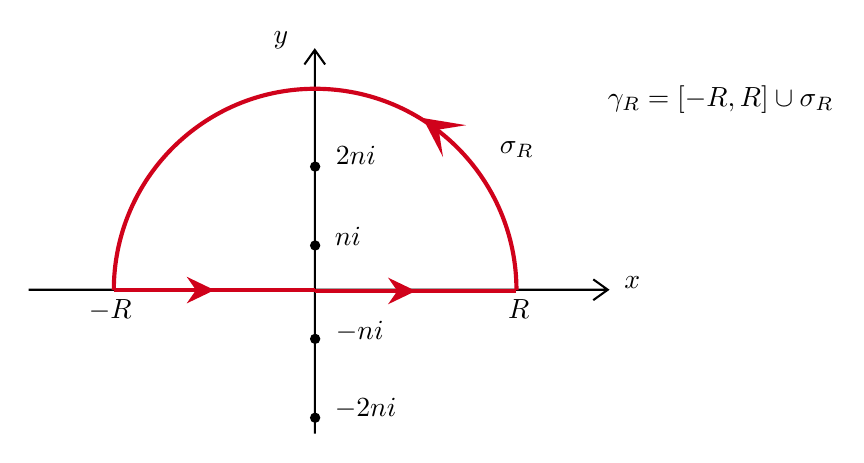
\begin{tikzpicture}[x=0.75pt,y=0.75pt,yscale=-1,xscale=1]
%uncomment if require: \path (0,224); %set diagram left start at 0, and has height of 224

%Shape: Axis 2D [id:dp7020002747782936] 
\draw  (112.5,140.17) -- (391.5,140.17)(250.33,24.63) -- (250.33,209.5) (384.5,135.17) -- (391.5,140.17) -- (384.5,145.17) (245.33,31.63) -- (250.33,24.63) -- (255.33,31.63)  ;
%Straight Lines [id:da8245049527209181] 
\draw [color={rgb, 255:red, 208; green, 2; blue, 27 }  ,draw opacity=1 ][line width=1.5]    (250.5,140.75) -- (347.5,140.75) ;
\draw [shift={(299,140.75)}, rotate = 180] [fill={rgb, 255:red, 208; green, 2; blue, 27 }  ,fill opacity=1 ][line width=0.08]  [draw opacity=0] (13.4,-6.43) -- (0,0) -- (13.4,6.44) -- (8.9,0) -- cycle    ;
%Shape: Arc [id:dp6724290607980123] 
\draw  [draw opacity=0][line width=1.5]  (153.5,140.33) .. controls (153.5,86.76) and (196.93,43.33) .. (250.5,43.33) .. controls (304.07,43.33) and (347.5,86.76) .. (347.5,140.33) -- (250.5,140.33) -- cycle ; \draw  [color={rgb, 255:red, 208; green, 2; blue, 27 }  ,draw opacity=1 ][line width=1.5]  (153.5,140.33) .. controls (153.5,86.76) and (196.93,43.33) .. (250.5,43.33) .. controls (304.07,43.33) and (347.5,86.76) .. (347.5,140.33) ;
%Straight Lines [id:da5477015911612453] 
\draw [color={rgb, 255:red, 208; green, 2; blue, 27 }  ,draw opacity=1 ][line width=1.5]    (153.5,140.33) -- (250.5,140.33) ;
\draw [shift={(202,140.33)}, rotate = 180] [fill={rgb, 255:red, 208; green, 2; blue, 27 }  ,fill opacity=1 ][line width=0.08]  [draw opacity=0] (13.4,-6.43) -- (0,0) -- (13.4,6.44) -- (8.9,0) -- cycle    ;
\draw  [draw opacity=0][fill={rgb, 255:red, 208; green, 2; blue, 27 }  ,fill opacity=1 ] (312.12,76.27) -- (302.31,57.43) -- (323.27,60.88) -- (310,63) -- cycle ;
%Shape: Circle [id:dp3205475558675792] 
\draw  [draw opacity=0][fill={rgb, 255:red, 0; green, 0; blue, 0 }  ,fill opacity=1 ] (248,80.83) .. controls (248,79.45) and (249.12,78.33) .. (250.5,78.33) .. controls (251.88,78.33) and (253,79.45) .. (253,80.83) .. controls (253,82.21) and (251.88,83.33) .. (250.5,83.33) .. controls (249.12,83.33) and (248,82.21) .. (248,80.83) -- cycle ;
%Shape: Circle [id:dp21100228306693403] 
\draw  [draw opacity=0][fill={rgb, 255:red, 0; green, 0; blue, 0 }  ,fill opacity=1 ] (248,118.83) .. controls (248,117.45) and (249.12,116.33) .. (250.5,116.33) .. controls (251.88,116.33) and (253,117.45) .. (253,118.83) .. controls (253,120.21) and (251.88,121.33) .. (250.5,121.33) .. controls (249.12,121.33) and (248,120.21) .. (248,118.83) -- cycle ;
%Shape: Circle [id:dp731209382058088] 
\draw  [draw opacity=0][fill={rgb, 255:red, 0; green, 0; blue, 0 }  ,fill opacity=1 ] (248,163.83) .. controls (248,162.45) and (249.12,161.33) .. (250.5,161.33) .. controls (251.88,161.33) and (253,162.45) .. (253,163.83) .. controls (253,165.21) and (251.88,166.33) .. (250.5,166.33) .. controls (249.12,166.33) and (248,165.21) .. (248,163.83) -- cycle ;
%Shape: Circle [id:dp8736348536667242] 
\draw  [draw opacity=0][fill={rgb, 255:red, 0; green, 0; blue, 0 }  ,fill opacity=1 ] (248,201.83) .. controls (248,200.45) and (249.12,199.33) .. (250.5,199.33) .. controls (251.88,199.33) and (253,200.45) .. (253,201.83) .. controls (253,203.21) and (251.88,204.33) .. (250.5,204.33) .. controls (249.12,204.33) and (248,203.21) .. (248,201.83) -- cycle ;

% Text Node
\draw (342,143.4) node [anchor=north west][inner sep=0.75pt]    {$R$};
% Text Node
\draw (398,132.4) node [anchor=north west][inner sep=0.75pt]    {$x$};
% Text Node
\draw (229,14.4) node [anchor=north west][inner sep=0.75pt]    {$y$};
% Text Node
\draw (140,143.4) node [anchor=north west][inner sep=0.75pt]    {$-R$};
% Text Node
\draw (338,67.4) node [anchor=north west][inner sep=0.75pt]    {$\sigma _{R}$};
% Text Node
\draw (390,40.4) node [anchor=north west][inner sep=0.75pt]    {$\gamma _{R} =[ -R,R] \cup \sigma _{R}$};
% Text Node
\draw (259,69.4) node [anchor=north west][inner sep=0.75pt]    {$2ni$};
% Text Node
\draw (258.5,108.4) node [anchor=north west][inner sep=0.75pt]    {$ni$};
% Text Node
\draw (259,153.9) node [anchor=north west][inner sep=0.75pt]    {$-ni$};
% Text Node
\draw (258.5,190.9) node [anchor=north west][inner sep=0.75pt]    {$-2ni$};


\end{tikzpicture}
\end{figure}
\FloatBarrier
\begin{equation*}
\begin{aligned}
I^{\star }_{n} & =2\pi i\cdotp \{\mathrm{Res}( g_{n} ,2ni) +\mathrm{Res}( g_{n} ,ni)\} =2\pi i\cdotp \left\{-\frac{i}{6n^{3}} +\frac{i}{12n^{3}}\right\}\\
I^{\star }_{n} & =\underbrace{\int _{\sigma _{R}} g( z) dz}_{\xrightarrow{R\rightarrow +\infty } 0} +\underbrace{\int ^{R}_{-R} g( z) dz}_{\xrightarrow{R\rightarrow +\infty } I_{n}}\\
 & \Rightarrow I_{n} =\frac{\pi }{6n^{3}}\\
 & \Rightarrow \Vert f_{n,\alpha } -F_{\alpha }\Vert _{L^{1}} =n^{\alpha } \cdotp \frac{\pi }{6n^{3}}\xrightarrow{n\rightarrow +\infty } 0\ \ \Leftrightarrow \ \ \alpha < 3\land \alpha \in [ 0,4)
\end{aligned}
\end{equation*}

Studiamo ora la norma $L^{\infty }$

Per $\alpha \in [ 0,4)$\begin{equation*}
\begin{aligned}
\Vert f_{n,\alpha } -F_{\alpha }\Vert _{L^{\infty }} & =\Vert f_{n,\alpha }\Vert _{L^{\infty }} & \\
 & =\max_{x\in \mathbb{R}} f_{n,\alpha }( x) & \left( f_{n} \ \text{sono continue e positive}\right)\\
 & =f_{n,\alpha }( 0) & \text{(simmetria)}\\
 & =\frac{1}{4n^{4-\alpha }}\xrightarrow{n\rightarrow +\infty } 0 & \\
 & \Rightarrow \ \ f_{n,\alpha }\xrightarrow[n\rightarrow +\infty ]{L^{\infty }(\mathbb{R})} F_{\alpha } & 
\end{aligned}
\end{equation*}Per $\alpha =4$\begin{equation*}
\begin{aligned}
\Vert f_{n,4} -F_{4}\Vert _{L^{\infty }} & =\left\Vert f_{n,4} -\frac{1}{4}\right\Vert _{L^{\infty }}\\
 & =\max_{x\in \mathbb{R}}\left[\frac{n^{4}}{\left( x^{2} +n^{2}\right)\left( x^{2} +4n^{2}\right)} -\frac{1}{4}\right]\\
 & =\frac{1}{4}\cancel{\xrightarrow{n\rightarrow +\infty }} 0\\
 & \Rightarrow \ \ f_{n,4}\cancel{\xrightarrow[n\rightarrow +\infty ]{L^{\infty }(\mathbb{R})}} F_{4}
\end{aligned}
\end{equation*}
\end{enumerate}
\Soluzione
\begin{theorem}
Sia $f:\mathbb{R}\rightarrow \mathbb{R}$, $T$-periodica, allora la serie di Fourier associata ad $f$ è\begin{equation*}
F( x) =\frac{a_{0}}{2} +\sum\limits ^{\infty }_{n=1}\left[ a_{n}\cos\left(\frac{2\pi n}{T} x\right) +b_{n}\sin\left(\frac{2\pi n}{T} x\right)\right]
\end{equation*}

dove
\begin{gather*}
a_{0} =\frac{2}{T}\int ^{\frac{T}{2}}_{-\frac{T}{2}} f( x) dx\\
a_{n} =\frac{2}{T}\int ^{\frac{T}{2}}_{-\frac{T}{2}} f( x)\cos\left(\frac{2\pi n}{T} x\right) dx\ \ \ \ b_{n} =\frac{2}{T}\int ^{\frac{T}{2}}_{-\frac{T}{2}} f( x)\sin\left(\frac{2\pi n}{T} x\right) dx
\end{gather*}
\textbf{NB.} Se $f$ è pari, il seno è dispari, $P\cdotp D=D\Rightarrow b_{n} =0\ \forall n\geqslant 1$.

\textbf{NB.} Se $f$ è dispari, il coseno è pari, $D\cdotp P=D\Rightarrow a_{n} =0\ \forall n\geqslant 0$.
\end{theorem}
\begin{enumerate}
\item Disegnamo la funzione

\begin{figure}[htpb]
	\centering
\tikzset{every picture/.style={line width=0.75pt}} %set default line width to 0.75pt        

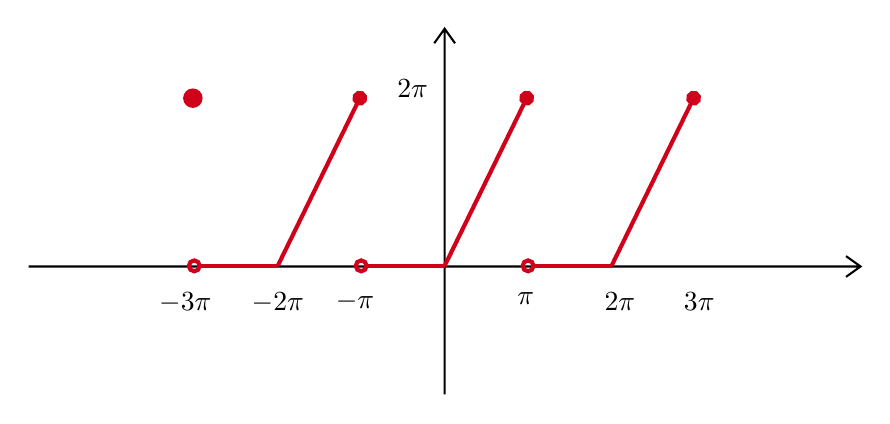
\begin{tikzpicture}[x=0.75pt,y=0.75pt,yscale=-1,xscale=1]
%uncomment if require: \path (0,198); %set diagram left start at 0, and has height of 198

%Shape: Axis 2D [id:dp24320808205526556] 
\draw  (100.11,120.97) -- (500.89,120.97)(300.5,6.41) -- (300.5,182.63) (493.89,115.97) -- (500.89,120.97) -- (493.89,125.97) (295.5,13.41) -- (300.5,6.41) -- (305.5,13.41)  ;
%Straight Lines [id:da6107470839046387] 
\draw [color={rgb, 255:red, 208; green, 2; blue, 27 }  ,draw opacity=1 ][line width=1.5]    (300.5,120.67) -- (340.04,39.87) ;
\draw [shift={(340.04,39.87)}, rotate = 296.08] [color={rgb, 255:red, 208; green, 2; blue, 27 }  ,draw opacity=1 ][fill={rgb, 255:red, 208; green, 2; blue, 27 }  ,fill opacity=1 ][line width=1.5]      (0, 0) circle [x radius= 2.61, y radius= 2.61]   ;
%Straight Lines [id:da4254536093640342] 
\draw [color={rgb, 255:red, 208; green, 2; blue, 27 }  ,draw opacity=1 ][line width=1.5]    (300.5,120.67) -- (261.9,120.67) ;
\draw [shift={(260.29,120.67)}, rotate = 180] [color={rgb, 255:red, 208; green, 2; blue, 27 }  ,draw opacity=1 ][line width=1.5]      (0, 0) circle [x radius= 2.61, y radius= 2.61]   ;

%Straight Lines [id:da07742835835652251] 
\draw [color={rgb, 255:red, 208; green, 2; blue, 27 }  ,draw opacity=1 ][line width=1.5]    (380.92,120.67) -- (420.46,39.87) ;
\draw [shift={(420.46,39.87)}, rotate = 296.08] [color={rgb, 255:red, 208; green, 2; blue, 27 }  ,draw opacity=1 ][fill={rgb, 255:red, 208; green, 2; blue, 27 }  ,fill opacity=1 ][line width=1.5]      (0, 0) circle [x radius= 2.61, y radius= 2.61]   ;
%Straight Lines [id:da9261529019653281] 
\draw [color={rgb, 255:red, 208; green, 2; blue, 27 }  ,draw opacity=1 ][line width=1.5]    (380.92,120.67) -- (342.32,120.67) ;
\draw [shift={(340.71,120.67)}, rotate = 180] [color={rgb, 255:red, 208; green, 2; blue, 27 }  ,draw opacity=1 ][line width=1.5]      (0, 0) circle [x radius= 2.61, y radius= 2.61]   ;

%Straight Lines [id:da5018794931536248] 
\draw [color={rgb, 255:red, 208; green, 2; blue, 27 }  ,draw opacity=1 ][line width=1.5]    (220.08,120.67) -- (259.62,39.87) ;
\draw [shift={(259.62,39.87)}, rotate = 296.08] [color={rgb, 255:red, 208; green, 2; blue, 27 }  ,draw opacity=1 ][fill={rgb, 255:red, 208; green, 2; blue, 27 }  ,fill opacity=1 ][line width=1.5]      (0, 0) circle [x radius= 2.61, y radius= 2.61]   ;
%Straight Lines [id:da10630889376486596] 
\draw [color={rgb, 255:red, 208; green, 2; blue, 27 }  ,draw opacity=1 ][line width=1.5]    (220.08,120.67) -- (181.48,120.67) ;
\draw [shift={(179.87,120.67)}, rotate = 180] [color={rgb, 255:red, 208; green, 2; blue, 27 }  ,draw opacity=1 ][line width=1.5]      (0, 0) circle [x radius= 2.61, y radius= 2.61]   ;

%Shape: Ellipse [id:dp5794600318678271] 
\draw  [draw opacity=0][fill={rgb, 255:red, 208; green, 2; blue, 27 }  ,fill opacity=1 ] (174.5,39.87) .. controls (174.5,37.28) and (176.6,35.18) .. (179.2,35.18) .. controls (181.79,35.18) and (183.89,37.28) .. (183.89,39.87) .. controls (183.89,42.46) and (181.79,44.57) .. (179.2,44.57) .. controls (176.6,44.57) and (174.5,42.46) .. (174.5,39.87) -- cycle ;

% Text Node
\draw (161.5,132.13) node [anchor=north west][inner sep=0.75pt]  [font=\normalsize]  {$-3\pi $};
% Text Node
\draw (206.07,132.13) node [anchor=north west][inner sep=0.75pt]  [font=\normalsize]  {$-2\pi $};
% Text Node
\draw (246.6,132.13) node [anchor=north west][inner sep=0.75pt]  [font=\normalsize]  {$-\pi $};
% Text Node
\draw (334.04,132.13) node [anchor=north west][inner sep=0.75pt]  [font=\normalsize]  {$\pi $};
% Text Node
\draw (376.1,132.13) node [anchor=north west][inner sep=0.75pt]  [font=\normalsize]  {$2\pi $};
% Text Node
\draw (414.3,132.13) node [anchor=north west][inner sep=0.75pt]  [font=\normalsize]  {$3\pi $};
% Text Node
\draw (276.25,29.26) node [anchor=north west][inner sep=0.75pt]  [font=\normalsize]  {$2\pi $};


\end{tikzpicture}
\end{figure}
\FloatBarrier

\item $f$ è regolare a tratti in $[ -\pi ,\pi ] \Rightarrow $ la serie di Fourier $F( x)$ converge puntualmente $\forall x\in \mathbb{R}$.
\begin{enumerate}
\item se $x$ è un punto di continuità, $F( x)$ converge a $f( x)$
\item se $x$ non è punto di continuità, $F( x)$ converge alla media tra il limite destro e sinistro
\end{enumerate}

nel nostro caso $f$ è continua in ogni punto $x\neq ( 2k+1) \pi ,k\in \mathbb{Z}$ e presenta delle discontinuità di I specie (tipo salto) nei punti $x=( 2k+1) \pi ,k\in \mathbb{Z}$.
\begin{enumerate}
\item $F( x)$ converge puntualmente a\begin{equation*}
f( x) \ \ \ \ \forall x\neq ( 2k+1) \pi ,k\in \mathbb{Z}
\end{equation*}
\item $F( x)$ converge puntualmente a\begin{equation*}
\frac{f\left( x^{+}\right) +f\left( x^{-}\right)}{2} =\frac{0+2\pi }{2} =\pi \ \ \ \ \forall x=( 2k+1) \pi ,k\in \mathbb{Z}
\end{equation*}
\end{enumerate}
\item Calcoliamo i coefficienti\begin{align*}
a_{0} & =\frac{2}{2\pi }\int ^{\pi }_{-\pi } f( x) dx=\frac{1}{\pi }\left\{\int ^{0}_{-\pi } f( x) dx+\int ^{\pi }_{0} f( x) dx\right\}\\
 & =\frac{1}{\pi }\int ^{\pi }_{0} f( x) dx=\frac{1}{\pi }\int ^{\pi }_{0} 2xdx=\frac{1}{\pi }\left[ x^{2}\right]^{\pi }_{0} =\frac{1}{\pi } \pi ^{2} =\textcolor[rgb]{0.82,0.01,0.11}{\pi }\\
 & \\
a_{n} & \overset{n\geqslant 1}{=}\frac{1}{\pi }\int ^{\pi }_{-\pi } f( x)\cos( nx) dx=\frac{1}{\pi }\int ^{\pi }_{0} 2x\cos( nx) dx\\
 & \\
 & \begin{array}{ l l }
h( x) =2x & h'( x) =2\\
g( x) =\frac{1}{n}\sin( nx) & g'( x) =\cos( nx)
\end{array}\\
 & \\
 & \overset{\text{ipp}}{=}\frac{1}{\pi }\left\{\left[\frac{2x}{n}\sin( nx)\right]^{\pi }_{0} -\int ^{\pi }_{0}\frac{2}{n}\sin( nx) dx\right\}\\
 & =\frac{1}{\pi }\left\{\cancel{\frac{2\pi }{n}\sin( n\pi )} -0+\left[\frac{2\cos( nx)}{n^{2}}\right]^{\pi }_{0}\right\}\\
 & =\frac{1}{\pi }\left\{\frac{2\cos( n\pi )}{n^{2}} -\frac{2}{n^{2}}\right\} =\frac{1}{\pi }\left\{\frac{2( -1)^{n}}{n^{2}} -\frac{2}{n^{2}}\right\}\\
 & =\textcolor[rgb]{0.82,0.01,0.11}{\frac{2}{\pi }}\textcolor[rgb]{0.82,0.01,0.11}{\frac{( -1)^{n} -1}{n^{2}}}\\
 & \\
b_{n} & =\frac{1}{\pi }\int ^{\pi }_{-\pi } f( x)\sin( nx) dx=\frac{1}{\pi }\int ^{\pi }_{0} 2x\sin( nx) dx\\
 & \\
 & \begin{array}{ l l }
k( x) =2x & k'( x) =2\\
r( x) =-\frac{1}{n}\cos( nx) & r'( x) =\sin( nx)
\end{array}\\
 & \\
 & \overset{\text{ipp}}{=}\frac{1}{\pi }\left\{\left[ -\frac{2x}{n}\cos( nx)\right]^{\pi }_{0} +\int ^{\pi }_{0}\frac{2}{n}\cos( nx) dx\right\}\\
 & =\frac{1}{\pi }\left\{-\frac{2\pi }{n}\cos( n\pi ) +0+\left[\frac{2\sin( nx)}{n^{2}}\right]^{\pi }_{0}\right\}\\
 & =\frac{1}{\pi }\left\{-\frac{2\pi }{n}( -1)^{n}\right\} =\textcolor[rgb]{0.82,0.01,0.11}{\frac{2}{n}}\textcolor[rgb]{0.82,0.01,0.11}{(}\textcolor[rgb]{0.82,0.01,0.11}{-1}\textcolor[rgb]{0.82,0.01,0.11}{)}\textcolor[rgb]{0.82,0.01,0.11}{^{n+1}}
\end{align*}

La serie di Fourier di $f$ è\begin{equation*}
F( x) =\frac{\pi }{2} +2\sum\limits ^{\infty }_{n=1}\left[\frac{( -1)^{n} -1}{\pi n^{2}}\cos( nx) +\frac{( -1)^{n+1}}{n}\sin( nx)\right]
\end{equation*}
\item Poiché $f\in L^{2}([ -\pi ,\pi ])$\begin{equation*}
\int ^{\pi }_{-\pi }| f( x)| ^{2} dx=\int ^{\pi }_{0}( 2x)^{2} dx=\int ^{\pi }_{0} 4x^{2} dx=\frac{4}{3} \pi ^{3} < +\infty 
\end{equation*}

allora $F( x)$ di $f$ converge in media quadratica.
\item Poiché $f$ \underline{\textbf{non}} è continua, allora la convergenza \underline{\textbf{non}} è uniforme su $\mathbb{R}$.
\end{enumerate}
\Soluzione
\begin{enumerate}
\item $f$ è pari $\Rightarrow b_{n} =0\ \forall n\in \mathbb{N}$\begin{equation*}
a_{k} =\frac{2}{\pi }\int ^{\frac{\pi }{2}}_{-\frac{\pi }{2}}\cos\left(\sqrt{2} x\right)\cos( 2kx) dx\ \ \forall k\in \mathbb{N}
\end{equation*}

modo $A$: calcolo per parti e ottengo un integrale ciclico.

modo $B$: usare la formula di Werner, usiamo questo\begin{equation*}
\cos \alpha \cos \beta =\frac{1}{2}[\cos( \alpha +\beta ) +\cos( \alpha -\beta )]
\end{equation*}

Procediamo al calcolo\begin{align*}
a_{k} & =\frac{\cancel{2}}{\pi }\int ^{\frac{\pi }{2}}_{-\frac{\pi }{2}}\frac{1}{\cancel{2}}\left\{\cos\left(\sqrt{2} x+2kx\right) +\cos\left(\sqrt{2} x-2kx\right)\right\} dx\\
 & =\frac{1}{\pi }\int ^{\frac{\pi }{2}}_{-\frac{\pi }{2}}\left\{\cos\left(\left(\sqrt{2} +2k\right) x\right) +\cos\left(\left(\sqrt{2} -2k\right) x\right)\right\} dx\\
 & =\frac{1}{\pi }\left\{\left[\frac{\sin\left(\left(\sqrt{2} +2k\right) x\right)}{\sqrt{2} +2k}\right]^{\frac{\pi }{2}}_{-\frac{\pi }{2}} +\left[\frac{\sin\left(\left(\sqrt{2} -2k\right) x\right)}{\sqrt{2} -2k}\right]^{\frac{\pi }{2}}_{-\frac{\pi }{2}}\right\}\\
 & =\frac{1}{\pi }\left\{\frac{\sin\left(\frac{\pi }{\sqrt{2}} +k\pi \right)}{\sqrt{2} +2k} +\frac{\sin\left(\frac{\pi }{\sqrt{2}} +k\pi \right)}{\sqrt{2} +2k} +\left[\frac{\sin\left(\left(\sqrt{2} -2k\right) x\right)}{\sqrt{2} -2k}\right]^{\frac{\pi }{2}}_{-\frac{\pi }{2}}\right\}\\
 & =\frac{1}{\pi }\left\{\frac{2\sin\left(\frac{\pi }{\sqrt{2}} +k\pi \right)}{\sqrt{2} +2k} +\frac{2\sin\left(\frac{\pi }{\sqrt{2}} -k\pi \right)}{\sqrt{2} -2k}\right\}\\
 & =\frac{2( -1)^{k}\sin\left(\frac{\pi }{\sqrt{2}}\right)}{\pi }\left(\frac{1}{\sqrt{2} +2k} +\frac{1}{\sqrt{2} -2k}\right)\\
 & =\frac{2( -1)^{k}\sin\left(\frac{\pi }{\sqrt{2}}\right)}{\pi }\left(\frac{1}{2k+\sqrt{2}} -\frac{1}{2k-\sqrt{2}}\right)\\
 & =-\frac{2\sqrt{2}( -1)^{k}\sin\left(\frac{\pi }{\sqrt{2}}\right)}{\pi \left( 2k^{2} -1\right)}
\end{align*}
\item La serie di Fourier di $f$ è\begin{equation*}
F( x) =\frac{a_{0}}{2} +\sum\limits ^{\infty }_{k=1} a_{k}\cos( 2kx)
\end{equation*}

per $x=\frac{\pi }{2}$\begin{equation*}
\begin{aligned}
F\left(\frac{\pi }{2}\right) & =\cos\left(\sqrt{2} \cdotp \frac{\pi }{2}\right) =\textcolor[rgb]{0.25,0.46,0.02}{\cos\left(\frac{\pi }{\sqrt{2}}\right)}\\
F\left(\frac{\pi }{2}\right) & =\frac{\sqrt{2}}{\pi }\sin\left(\frac{\pi }{\sqrt{2}}\right) +\sum\limits ^{\infty }_{k=1} a_{k}( -1)^{k}\\
 & =\textcolor[rgb]{0.74,0.06,0.88}{\frac{\sqrt{2}}{\pi }\sin\left(\frac{\pi }{\sqrt{2}}\right)}\textcolor[rgb]{0.96,0.65,0.14}{-\frac{2\sqrt{2}\sin\left(\frac{\pi }{\sqrt{2}}\right)}{\pi }}\sum\limits ^{\infty }_{k=1}\frac{( -1)^{k}( -1)^{k}}{\left( 2k^{2} -1\right)}\\
 & \\
\Rightarrow \ \ \sum\limits ^{\infty }_{k=1}\frac{1}{\left( 2k^{2} -1\right)} & =\frac{\textcolor[rgb]{0.25,0.46,0.02}{\cos\left(\frac{\pi }{\sqrt{2}}\right)} -\textcolor[rgb]{0.74,0.06,0.88}{\frac{\sqrt{2}}{\pi }\sin\left(\frac{\pi }{\sqrt{2}}\right)}}{\textcolor[rgb]{0.96,0.65,0.14}{-\frac{2\sqrt{2}\sin\left(\frac{\pi }{\sqrt{2}}\right)}{\pi }}} =-\frac{\textcolor[rgb]{0.25,0.46,0.02}{\cos\left(\frac{\pi }{\sqrt{2}}\right)}}{\textcolor[rgb]{0.96,0.65,0.14}{\frac{2\sqrt{2}\sin\left(\frac{\pi }{\sqrt{2}}\right)}{\pi }}} +\frac{\textcolor[rgb]{0.74,0.06,0.88}{\frac{\sqrt{2}}{\pi }\sin\left(\frac{\pi }{\sqrt{2}}\right)}}{\textcolor[rgb]{0.96,0.65,0.14}{\frac{2\sqrt{2}\sin\left(\frac{\pi }{\sqrt{2}}\right)}{\pi }}}\\
 & =-\frac{\pi }{2\sqrt{2}}\cot\left(\frac{\pi }{\sqrt{2}}\right) +\frac{1}{2}
\end{aligned}
\end{equation*}
\item $f\in L^{2}\left(\left[ -\frac{\pi }{2} ,\frac{\pi }{2}\right]\right) \Rightarrow $ ho convergenza in media quadratica

Criterio di Weierstrass, prendo il termine generale in modulo\begin{gather*}
| a_{k}\cos( 2k\pi )| \leqslant \frac{2\sqrt{2}}{\pi \left( 2k^{2} -1\right)}\\
\sum\limits ^{\infty }_{k=1}\frac{2\sqrt{2}}{\pi \left( 2k^{2} -1\right)} < +\infty \ \ \Rightarrow \ \ \text{convergenza è uniforme su} \ \mathbb{R}
\end{gather*}
\end{enumerate}
\chapter{Esercitazione 6 - Boella}
\ParteEsercizi
\Esercizio{}

Data una funzione $2\pi $-periodica
\begin{equation*}
f:[ -\pi ,\pi ]\rightarrow \mathbb{R} \ \ \ \ f(x)=x^{2}
\end{equation*}
Determinare la sue serie di Fourier. Si riesce a ricondurre la serie ad una nota?
\Esercizio{}

Data una funzione $3$-periodica
\begin{equation*}
f(x)=\begin{cases}
0, & 0\leq x< 1\\
1, & 1\leq x< 2\\
2, & 2\leq x< 3
\end{cases}
\end{equation*}
Determinare la sue serie di Fourier. Si riesce a ricondurre la serie ad una nota?
\Esercizio{}
\begin{definition}
[Spazio delle funzioni test] $\varphi \in D( A)$ se $\varphi \in C^{\infty }( A)$, $\exists K$ compatto tale per cui $\varphi ( x) =0,\forall x\notin K$
\end{definition}
\textit{Esempio.}
\begin{equation*}
\varphi ( x) =\begin{cases}
e^{-\frac{1}{1-x^{2}}} , & | x| < 1\\
0, & | x| \geqslant 1
\end{cases}
\end{equation*}
\fg{0.7}{11-3-1}
\begin{definition}
[Distribuzione] Si chiamano distribuzioni gli oggetti $T\in D'( A)$. $T$ è un funzionale lineare continuo su $D( A)$. Quindi so dire cosa fa $T$ a una funzione test $\varphi $ tramite il prodotto di dualità
\begin{equation*}
T( \varphi ) =\langle T,\varphi \rangle 
\end{equation*}
\end{definition}
\begin{definition}
[Convergenza di funzioni test] Diciamo che $\varphi _{k}\xrightarrow{D( A)} \varphi $ se $\forall \alpha ,D^{\alpha } \varphi _{k}\rightarrow D^{\alpha } \varphi $.
\end{definition}
\begin{definition}
[Prodotto di dualità] Data $T\in D'( A)$, se $T\in L^{1}_{\mathrm{loc}}( A) \Rightarrow \langle T,\varphi \rangle =\int _{A} T( x) \varphi ( x) dx$. Se invece $T\notin L^{1}_{\mathrm{loc}} \Rightarrow \langle T,\varphi \rangle $ lo dobbiamo definire manualmente, per esempio la Delta di Dirac che è definita come
\begin{equation*}
\langle \delta ,\varphi \rangle =\varphi ( 0)
\end{equation*}
Possiamo anche traslarla
\begin{equation*}
\langle \delta _{x_{0}} ,\varphi \rangle =\varphi ( x_{0})
\end{equation*}
\end{definition}
\begin{definition}
[Convergenza di distribuzioni] Diciamo che $T_{n}\xrightarrow{D'( A)} T$ se $\langle T_{n} ,\varphi \rangle \rightarrow \langle T,\varphi \rangle $, $\forall \varphi \in D( A)$.
\end{definition}
Studiare la convergenza in distribuzione della seguente successione
\begin{equation*}
f_{n} (x)=ne^{-n|x|}
\end{equation*}
\Esercizio{}

Studiare la convergenza in distribuzione della seguente successione
\begin{equation*}
f_{n} (x)=\begin{cases}
-3n, & |x|\leq \frac{1}{n}\\
2n, & \frac{1}{n} < |x|\leq \frac{2}{n}\\
0, & |x| >\frac{2}{n}
\end{cases}
\end{equation*}
\Esercizio{}

Studiare la convergenza in distribuzione della seguente successione
\begin{equation*}
f_{n} (x)=nx^{n} \chi _{(0,1)} (x)
\end{equation*}
\ParteSoluzioni
\Soluzione

Osserviamo che la funzione $f(x)=x^{2}$ converge in $L^{2}$ e puntualmente su $\mathbb{R}$.

Osserviamo che $b_{n} =0,\forall n$ perché la funzione è pari.

Calcoliamo ora $a_{0}$ e $a_{n}$:
\begin{align*}
a_{0} & =\frac{1}{\pi }\int ^{\pi }_{-\pi } f(x)dx=\frac{2}{\pi }\int ^{\pi }_{0} f(x)dx=\frac{2}{3} \pi ^{2}\\
 & \\
a_{n} & =\frac{1}{\pi }\int ^{\pi }_{-\pi } f(x)\cos( nx) dx\\
 & =\frac{2}{\pi }\int ^{\pi }_{0} f(x)\cos (nx)dx\\
 & =\frac{2}{\pi }\int ^{\pi }_{0} x^{2}\cos (nx)dx\\
 & \overset{\text{ipp}}{=}\frac{2}{\pi }\left\{\cancel{\left[ x^{2}\frac{\sin (nx)}{n}\right]^{\pi }_{0}} -\frac{2}{n}\int ^{\pi }_{0} x\sin (nx)dx\right\}\\
 & \overset{\text{ipp}}{=} -\frac{4}{n\pi }\left\{\left[ -\frac{x}{n}\cos( nx)\right]^{\pi }_{0} +\cancel{\frac{1}{n}\int ^{\pi }_{0}\cos( nx) dx}\right\}\\
 & =\frac{4}{n\pi } \cdotp \frac{\pi }{n}\cos( n\pi ) =\frac{4}{n^{2}}( -1)^{n}
\end{align*}
La serie di Fourier cercata è:
\begin{equation*}
f(x)=\frac{\pi ^{2}}{3} +\sum ^{\infty }_{n=1} (-1)^{n}\frac{4}{n^{2}}\cos (nx)
\end{equation*}
Inoltre
\begin{equation*}
\sum ^{\infty }_{n=1}( |a_{n} |+|b_{n} |) < \infty \ \ \Rightarrow \ \ \text{c'è anche convergenza uniforme}
\end{equation*}
Ricaviamo alcune serie notevoli.
\begin{itemize}
\item in $x=\pi $\begin{gather*}
\pi ^{2} =f( \pi ) =\frac{\pi ^{2}}{3} +\sum ^{\infty }_{n=1} (-1)^{n}\frac{4}{n^{2}}\cos (n\pi )=\frac{\pi ^{2}}{3} +4\sum ^{\infty }_{n=1}\frac{1}{n^{2}}\\
\Rightarrow \ \ \boxed{\sum ^{\infty }_{n=1}\frac{1}{n^{2}} =\frac{\pi ^{2}}{6}}
\end{gather*}
\item in $x=0$\begin{gather*}
0=f( 0) =\frac{\pi ^{2}}{3} +\sum ^{\infty }_{n=1} (-1)^{n}\frac{4}{n^{2}}\cos (0)=\frac{\pi ^{2}}{3} +4\sum ^{\infty }_{n=1}\frac{(-1)^{n}}{n^{2}}\\
\Rightarrow \ \ \boxed{\sum ^{\infty }_{n=1}\frac{(-1)^{n}}{n^{2}} =-\frac{\pi ^{2}}{12}}
\end{gather*}
\item Parseval\begin{equation*}
\int ^{2\pi }_{0}[ f(x)]^{2} dx=\pi \left[\frac{a^{2}_{0}}{2} +\sum ^{\infty }_{n=1} (a^{2}_{n} +b^{2}_{n} )\right]
\end{equation*}

Allora\begin{equation*}
\begin{aligned}
\int ^{\pi }_{-\pi }\left( x^{2}\right)^{2} dx & =\pi \left[\frac{\left(\frac{2}{3} \pi ^{2}\right)^{2}}{2} +\sum\limits ^{\infty }_{n=1}\frac{16}{n^{4}}\right]\\
2\cdotp \frac{\pi ^{5}}{5} & =\pi \left[\frac{2}{9} \pi ^{4} +16\sum\limits ^{\infty }_{n=1}\frac{1}{n^{4}}\right]\\
\left(\frac{2}{5} -\frac{2}{9}\right) \pi ^{4} & =16\sum\limits ^{\infty }_{n=1}\frac{1}{n^{4}} \ \ \Rightarrow \ \ \boxed{\sum\limits ^{\infty }_{n=1}\frac{1}{n^{4}} =\frac{\pi ^{4}}{90}}
\end{aligned}
\end{equation*}
\end{itemize}
\Soluzione

Iniziamo osservando che la funzione
\begin{equation*}
f(x)=\begin{cases}
0, & 0\leq x< 1\\
1, & 1\leq x< 2\\
2, & 2\leq x< 3
\end{cases}
\end{equation*}
converge in $L^{2}( 0,3)$. Converge inoltre puntualmente q.o. su $\mathbb{R}$ (a meno dell'insieme $x\notin \mathbb{Z}$).


\begin{figure}[htpb]
	\centering
\tikzset{every picture/.style={line width=0.75pt}} %set default line width to 0.75pt        

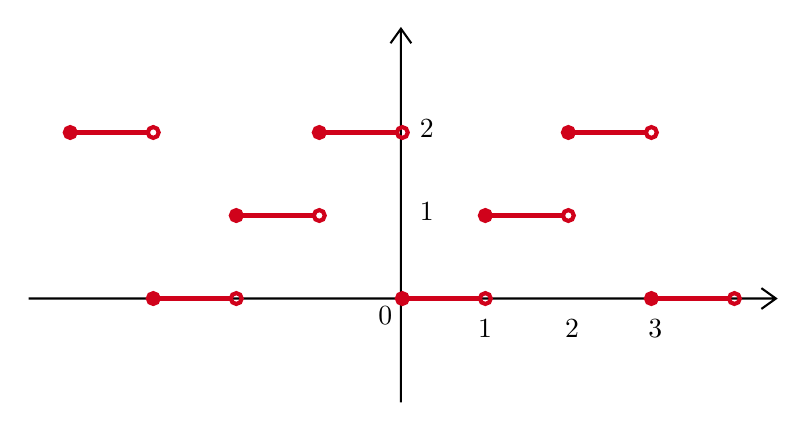
\begin{tikzpicture}[x=0.75pt,y=0.75pt,yscale=-1,xscale=1]
%uncomment if require: \path (0,214); %set diagram left start at 0, and has height of 214

%Shape: Axis 2D [id:dp9173052200245366] 
\draw  (120,150) -- (480,150)(299.33,20) -- (299.33,200) (473,145) -- (480,150) -- (473,155) (294.33,27) -- (299.33,20) -- (304.33,27)  ;
%Straight Lines [id:da6842800458327545] 
\draw [color={rgb, 255:red, 208; green, 2; blue, 27 }  ,draw opacity=1 ][line width=1.5]    (300,150) -- (338.39,150) ;
\draw [shift={(340,150)}, rotate = 0] [color={rgb, 255:red, 208; green, 2; blue, 27 }  ,draw opacity=1 ][line width=1.5]      (0, 0) circle [x radius= 2.61, y radius= 2.61]   ;
\draw [shift={(300,150)}, rotate = 0] [color={rgb, 255:red, 208; green, 2; blue, 27 }  ,draw opacity=1 ][fill={rgb, 255:red, 208; green, 2; blue, 27 }  ,fill opacity=1 ][line width=1.5]      (0, 0) circle [x radius= 2.61, y radius= 2.61]   ;
%Straight Lines [id:da3441135935225803] 
\draw [color={rgb, 255:red, 208; green, 2; blue, 27 }  ,draw opacity=1 ][line width=1.5]    (340,110) -- (378.39,110) ;
\draw [shift={(380,110)}, rotate = 0] [color={rgb, 255:red, 208; green, 2; blue, 27 }  ,draw opacity=1 ][line width=1.5]      (0, 0) circle [x radius= 2.61, y radius= 2.61]   ;
\draw [shift={(340,110)}, rotate = 0] [color={rgb, 255:red, 208; green, 2; blue, 27 }  ,draw opacity=1 ][fill={rgb, 255:red, 208; green, 2; blue, 27 }  ,fill opacity=1 ][line width=1.5]      (0, 0) circle [x radius= 2.61, y radius= 2.61]   ;
%Straight Lines [id:da03802847326309822] 
\draw [color={rgb, 255:red, 208; green, 2; blue, 27 }  ,draw opacity=1 ][line width=1.5]    (380,70) -- (418.39,70) ;
\draw [shift={(420,70)}, rotate = 0] [color={rgb, 255:red, 208; green, 2; blue, 27 }  ,draw opacity=1 ][line width=1.5]      (0, 0) circle [x radius= 2.61, y radius= 2.61]   ;
\draw [shift={(380,70)}, rotate = 0] [color={rgb, 255:red, 208; green, 2; blue, 27 }  ,draw opacity=1 ][fill={rgb, 255:red, 208; green, 2; blue, 27 }  ,fill opacity=1 ][line width=1.5]      (0, 0) circle [x radius= 2.61, y radius= 2.61]   ;
%Straight Lines [id:da9565199441833196] 
\draw [color={rgb, 255:red, 208; green, 2; blue, 27 }  ,draw opacity=1 ][line width=1.5]    (180,150) -- (218.39,150) ;
\draw [shift={(220,150)}, rotate = 0] [color={rgb, 255:red, 208; green, 2; blue, 27 }  ,draw opacity=1 ][line width=1.5]      (0, 0) circle [x radius= 2.61, y radius= 2.61]   ;
\draw [shift={(180,150)}, rotate = 0] [color={rgb, 255:red, 208; green, 2; blue, 27 }  ,draw opacity=1 ][fill={rgb, 255:red, 208; green, 2; blue, 27 }  ,fill opacity=1 ][line width=1.5]      (0, 0) circle [x radius= 2.61, y radius= 2.61]   ;
%Straight Lines [id:da9765401043379787] 
\draw [color={rgb, 255:red, 208; green, 2; blue, 27 }  ,draw opacity=1 ][line width=1.5]    (220,110) -- (258.39,110) ;
\draw [shift={(260,110)}, rotate = 0] [color={rgb, 255:red, 208; green, 2; blue, 27 }  ,draw opacity=1 ][line width=1.5]      (0, 0) circle [x radius= 2.61, y radius= 2.61]   ;
\draw [shift={(220,110)}, rotate = 0] [color={rgb, 255:red, 208; green, 2; blue, 27 }  ,draw opacity=1 ][fill={rgb, 255:red, 208; green, 2; blue, 27 }  ,fill opacity=1 ][line width=1.5]      (0, 0) circle [x radius= 2.61, y radius= 2.61]   ;
%Straight Lines [id:da7209581982756688] 
\draw [color={rgb, 255:red, 208; green, 2; blue, 27 }  ,draw opacity=1 ][line width=1.5]    (260,70) -- (298.39,70) ;
\draw [shift={(300,70)}, rotate = 0] [color={rgb, 255:red, 208; green, 2; blue, 27 }  ,draw opacity=1 ][line width=1.5]      (0, 0) circle [x radius= 2.61, y radius= 2.61]   ;
\draw [shift={(260,70)}, rotate = 0] [color={rgb, 255:red, 208; green, 2; blue, 27 }  ,draw opacity=1 ][fill={rgb, 255:red, 208; green, 2; blue, 27 }  ,fill opacity=1 ][line width=1.5]      (0, 0) circle [x radius= 2.61, y radius= 2.61]   ;
%Straight Lines [id:da15781035361747886] 
\draw [color={rgb, 255:red, 208; green, 2; blue, 27 }  ,draw opacity=1 ][line width=1.5]    (140,70) -- (178.39,70) ;
\draw [shift={(180,70)}, rotate = 0] [color={rgb, 255:red, 208; green, 2; blue, 27 }  ,draw opacity=1 ][line width=1.5]      (0, 0) circle [x radius= 2.61, y radius= 2.61]   ;
\draw [shift={(140,70)}, rotate = 0] [color={rgb, 255:red, 208; green, 2; blue, 27 }  ,draw opacity=1 ][fill={rgb, 255:red, 208; green, 2; blue, 27 }  ,fill opacity=1 ][line width=1.5]      (0, 0) circle [x radius= 2.61, y radius= 2.61]   ;
%Straight Lines [id:da6022039956275556] 
\draw [color={rgb, 255:red, 208; green, 2; blue, 27 }  ,draw opacity=1 ][line width=1.5]    (420,150) -- (458.39,150) ;
\draw [shift={(460,150)}, rotate = 0] [color={rgb, 255:red, 208; green, 2; blue, 27 }  ,draw opacity=1 ][line width=1.5]      (0, 0) circle [x radius= 2.61, y radius= 2.61]   ;
\draw [shift={(420,150)}, rotate = 0] [color={rgb, 255:red, 208; green, 2; blue, 27 }  ,draw opacity=1 ][fill={rgb, 255:red, 208; green, 2; blue, 27 }  ,fill opacity=1 ][line width=1.5]      (0, 0) circle [x radius= 2.61, y radius= 2.61]   ;

% Text Node
\draw (335,158.9) node [anchor=north west][inner sep=0.75pt]    {$1$};
% Text Node
\draw (377,158.9) node [anchor=north west][inner sep=0.75pt]    {$2$};
% Text Node
\draw (417,158.9) node [anchor=north west][inner sep=0.75pt]    {$3$};
% Text Node
\draw (307,102.4) node [anchor=north west][inner sep=0.75pt]    {$1$};
% Text Node
\draw (307,62.4) node [anchor=north west][inner sep=0.75pt]    {$2$};
% Text Node
\draw (287,152.4) node [anchor=north west][inner sep=0.75pt]    {$0$};


\end{tikzpicture}
\end{figure}
\FloatBarrier

\begin{equation*}
f( x) \sim \frac{a_{0}}{2} +\sum\limits ^{\infty }_{n=1}\left[ a_{n}\cos\left(\frac{2n\pi }{3} x\right) +b_{n}\sin\left(\frac{2n\pi }{3} x\right)\right]
\end{equation*}
Calcoliamo ora i coefficienti:
\begin{align*}
a_{0} & =\frac{1}{3/2}\int ^{3}_{0} f(x)dx=\frac{2}{3} \cdotp 3=2\\
 & \\
a_{n} & =\frac{1}{3/2}\int ^{3}_{0} f(x)\cos\left(\frac{2n\pi }{3}\right) dx=\frac{2}{3}\left\{\int ^{2}_{1} 1\cos\left(\frac{2n\pi }{3}\right) dx+\int ^{3}_{2} 2\cos\left(\frac{2n\pi }{3}\right) dx\right\}\\
 & =\frac{2}{3}\left\{\left[\frac{3}{2n\pi }\sin\left(\frac{2n\pi }{3} x\right)\right]^{2}_{1} +2\left[\frac{3}{2n\pi }\sin\left(\frac{2n\pi }{3} x\right)\right]^{3}_{2}\right\}\\
 & =\frac{2}{3}\frac{3}{2n\pi }\left\{\sin\left(\frac{4n\pi }{3}\right) -\sin\left(\frac{2n\pi }{3}\right) +\cancel{2\sin( 2n\pi )} -2\sin\left(\frac{4n\pi }{3}\right)\right\} =0,\ \forall n\\
 & \\
b_{n} & =\frac{2}{3}\int ^{3}_{0} f(x)\sin\left(\frac{2n\pi }{3}\right) dx=\frac{2}{3}\left\{\int ^{2}_{1} 1\sin\left(\frac{2n\pi }{3}\right) dx+\int ^{3}_{2} 2\sin\left(\frac{2n\pi }{3}\right) dx\right\}\\
 & =\frac{2}{3}\frac{3}{2n\pi }\left\{\left[ -\cos\left(\frac{2n\pi }{3}\right)\right]^{2}_{1} -2\left[\cos\left(\frac{2n\pi }{3}\right)\right]^{3}_{2}\right\}\\
 & =-\frac{1}{n\pi }\left\{\cos\left(\frac{4n\pi }{3}\right) -\cos\left(\frac{2n\pi }{3}\right) +2\cos( 2n\pi ) -2\cos\left(\frac{4n\pi }{3}\right)\right\}\\
 & =-\frac{1}{n\pi } \cdotp \begin{cases}
1, & n=1,4,7,\dotsc \\
1, & n=2,5,8,\dotsc \\
0, & \text{altrimenti}
\end{cases} =\begin{cases}
0, & n=3k,k\in \mathbb{Z}\\
-\frac{1}{n\pi } , & \text{altrimenti}
\end{cases}
\end{align*}
La serie cercata è:
\begin{equation*}
f(x)=1+\sum ^{\infty }_{n=1} b_{n}\sin\left(\frac{2n\pi }{3} x\right)
\end{equation*}
La funzione è una funzione dispari traslata di $1$ verso l'alto.
\Soluzione

Limite puntuale
\begin{equation*}
f_{n} (x)=ne^{-n|x|} \ \ \ \ \lim\limits _{n\rightarrow +\infty } f_{n}( x) =\begin{cases}
0, & x\neq 0\\
+\infty , & x=0
\end{cases} \ \ \Rightarrow \ \ f_{n}\xrightarrow{\text{q.o.}} F( x) \equiv 0
\end{equation*}
\fg{0.7}{11-3}

Notiamo che non c'è convergenza in $L^{1}$:
\begin{equation*}
\Vert f_{n} -F\Vert _{L^{1}(\mathbb{R})} =2\int ^{\infty }_{0} ne^{-nx} dx=2\left[ -e^{-nx}\right]^{\infty }_{0} =2\nrightarrow 0
\end{equation*}
Tuttavia $f_{n} \in L^{1}_{\mathrm{loc}}(\mathbb{R})$, quindi sono anche associate a una distribuzione.
\begin{equation*}
\begin{aligned}
\langle f_{n} ,\varphi \rangle  & =\int _{\mathbb{R}} ne^{-n| x| } \varphi ( x) dx=\int ^{0}_{-\infty } ne^{nx} \varphi ( x) dx+\int ^{\infty }_{0} ne^{-nx} \varphi ( x) dx\\
 & \overset{\text{ipp}}{=}\left[ e^{nx} \varphi ( x)\right]^{0}_{-\infty } -\int ^{0}_{-\infty } e^{nx} \varphi '( x) dx+\left[ -e^{-nx}\right]^{\infty }_{0} +\int ^{\infty }_{0} e^{-nx} \varphi '( x) dx\\
 & =\varphi ( 0) -\underbrace{\int ^{0}_{-\infty } e^{nx} \varphi '( x) dx}_{\xrightarrow{\text{Dom}} 0} +\varphi ( 0) +\underbrace{\int ^{\infty }_{0} e^{-nx} \varphi '( x) dx}_{\xrightarrow{\text{Dom}} 0}\rightarrow 2\varphi ( 0)
\end{aligned}
\end{equation*}
Prendiamo $g_{n}( x) =e^{-nx} \varphi '( x)$ su $( 0,+\infty )$, $g_{n}( x)\rightarrow 0$ puntualmente, inoltre
\begin{equation*}
| \varphi '( x)| \leqslant K\ \ \Rightarrow \ \ | g_{n}( x)| \leqslant Ke^{-x} \in L^{1}( 0,+\infty )
\end{equation*}
Quindi
\begin{equation*}
\langle f_{n} ,\varphi \rangle \rightarrow 2\varphi ( 0) =2\langle \delta ,\varphi \rangle \ \ \Rightarrow \ \ f_{n}\xrightarrow{D'(\mathbb{R})} 2\delta 
\end{equation*}
\Soluzione

Limite puntuale
\begin{equation*}
\lim\limits _{n\rightarrow +\infty } f_{n}( x) =\begin{cases}
-\infty , & x=0\\
0, & x\neq 0
\end{cases} \ \ \Rightarrow \ \ f_{n}\xrightarrow{\text{q.o.}} F( x) \equiv 0
\end{equation*}
\fg{0.7}{11-4}

In $D'(\mathbb{R})$
\begin{equation*}
\begin{aligned}
\langle f_{n} ,\varphi \rangle  & =\int ^{-1/n}_{-2/n} 2n\varphi ( x) dx+\int ^{1/n}_{-1/n}( -3n) \varphi ( x) dx+\int ^{2/n}_{1/n} 2n\varphi ( x) dx\\
 & =2n\int ^{-1/n}_{-2/n} \varphi ( x) dx-3n\int ^{1/n}_{-1/n} \varphi ( x) dx+2n\int ^{2/n}_{1/n} \varphi ( x) dx
\end{aligned}
\end{equation*}
Per le funzioni continue, e le $\varphi $ lo sono, vale il teorema della media
\begin{equation*}
\int ^{b}_{a} \varphi ( x) dx=( b-a) \varphi ( c)
\end{equation*}
Allora
\begin{equation*}
\begin{aligned}
\langle f_{n} ,\varphi \rangle  & =2n\int ^{-1/n}_{-2/n} \varphi ( x) dx-3n\int ^{1/n}_{-1/n} \varphi ( x) dx+2n\int ^{2/n}_{1/n} \varphi ( x) dx\\
 & =2n\left(\frac{-1}{n} -\frac{-2}{n}\right) \varphi ( \alpha _{n}) -3n\left(\frac{1}{n} -\frac{-1}{n}\right) \varphi ( \beta _{n}) +2n\left(\frac{2}{n} -\frac{1}{n}\right) \varphi ( \gamma _{n})
\end{aligned}
\end{equation*}
dove
\begin{equation*}
-\frac{2}{n} \leqslant \alpha _{n} \leqslant -\frac{1}{n} \leqslant \beta _{n} \leqslant \frac{1}{n} \leqslant \gamma _{n} \leqslant \frac{2}{n}
\end{equation*}
procediamo coi calcoli
\begin{equation*}
\begin{aligned}
\langle f_{n} ,\varphi \rangle  & =2n\left(\frac{-1}{n} -\frac{-2}{n}\right) \varphi ( \alpha _{n}) -3n\left(\frac{1}{n} -\frac{-1}{n}\right) \varphi ( \beta _{n}) +2n\left(\frac{2}{n} -\frac{1}{n}\right) \varphi ( \gamma _{n})\\
 & =2\varphi ( \alpha _{n}) -6\varphi ( \beta _{n}) +2\varphi ( \gamma _{n})\xrightarrow{n\rightarrow +\infty } 2\varphi ( 0) -6\varphi ( 0) +2\varphi ( 0) =-2\varphi ( 0)
\end{aligned}
\end{equation*}
Facendo lo stesso gioco su una funzione
\begin{equation*}
g_{n} (x)=\begin{cases}
-n, & |x|\leq \frac{1}{n}\\
2n, & \frac{1}{n} < |x|\leq \frac{2}{n}\\
0, & |x| >\frac{2}{n}
\end{cases} \ \ \Rightarrow \ \ G( x) \equiv 0
\end{equation*}
viene
\begin{equation*}
\langle g_{n} ,\varphi \rangle =2\varphi ( \alpha _{n}) -2\varphi ( \beta _{n}) +2\varphi ( \gamma _{n})\rightarrow 2\varphi ( 0)
\end{equation*}
Ovvero
\begin{equation*}
f_{n}\xrightarrow{D'(\mathbb{R})} -2\delta \ \ \ \ g_{n}\xrightarrow{D'(\mathbb{R})} 2\delta 
\end{equation*}
\Soluzione

Limite puntuale
\begin{equation*}
f_{n} (x)=nx^{n} \chi _{(0,1)} (x)\ \ \ \ \lim\limits _{n\rightarrow +\infty } f_{n}( x) =0,\ \forall x\in \mathbb{R}
\end{equation*}
\fg{0.3}{11-5}
\begin{equation*}
\begin{aligned}
\langle f_{n} ,\varphi \rangle  & =\int ^{1}_{0} nx^{n} \varphi ( x) dx\overset{\text{ipp}}{=}\left[\frac{n}{n+1} x^{n+1} \varphi ( x)\right]^{1}_{0} -\int ^{1}_{0}\frac{n}{n+1} x^{n+1} \varphi '( x) dx\\
 & =\frac{n}{n+1} \varphi ( 1) -\frac{n}{n+1}\underbrace{\int ^{1}_{0} x^{n+1} \varphi '( x) dx}_{\xrightarrow{\text{Dom}} 0}\xrightarrow{n\rightarrow +\infty } \varphi ( 1)
\end{aligned}
\end{equation*}
Dato che $g_{n}( x) =x^{n+1} \varphi '( x)\xrightarrow{n\rightarrow +\infty } 0,\ \forall x\in ( 0,1)$
\begin{equation*}
| g_{n}( x)| \leqslant \varphi '( x) \in L^{1}
\end{equation*}
In conclusione
\begin{equation*}
\langle f_{n} ,\varphi \rangle \rightarrow \langle \delta _{1} ,\varphi \rangle \ \ \Rightarrow \ \ f_{n}\xrightarrow{D'(\mathbb{R})} \delta _{1}
\end{equation*}
\textit{Esercizio per casa.}

Date $f_{n}( x) =nx^{n} \chi _{( 0,1)}( x)$, calcolare il limite in $D'( 0,1)$.
\chapter{Esercitazione 6 - Potrich}
\ParteEsercizi
\Esercizio{}

Sia $f:\mathbb{R}\rightarrow \mathbb{R}$ la funzione $2\pi $-periodica dispari definita da
\begin{equation*}
f( x) =\begin{cases}
\sin x, & x\in \left[ 0,\frac{\pi }{2}\right)\\
0, & x\in \left[\frac{\pi }{2} ,\pi \right]
\end{cases}
\end{equation*}
\begin{enumerate}
\item Disegnare il grafico di $f$ su $[ -3\pi ,3\pi ]$
\item Stabilire se la serie di Fourier di $f$ converge in media quadratica.
\item Stabilire se la serie di Fourier converge puntualmente.
\item Stabilire se la serie di Fourier converge uniformemente.
\item Scrivere la serie di Fourier di $f$.
\item Dire che cosa accade per $x=\frac{\pi }{4}$ e calcolare\begin{equation*}
\sum\limits ^{\infty }_{n=0}( -1)^{n}\frac{2n+1}{4( 2n+1)^{2} -1}
\end{equation*}
\item Scrivere l'identità di Parseval per $f$ e sfruttarla per calcolare\begin{equation*}
\sum\limits ^{\infty }_{n=1}\frac{n^{2}}{\left( 4n^{2} -1\right)^{2}}
\end{equation*}
\end{enumerate}
\Esercizio{}

Sia $Q=[ -\pi ,\pi )$ e $F( x)$ lo sviluppo in serie di Fourier di $f( x) =| x| ,\ \forall x\in Q$. Calcolare
\begin{equation*}
\sum\limits ^{\infty }_{n=0}\frac{1}{( 2n+1)^{4}} \ \ \ \ \sum\limits ^{\infty }_{n=1}\frac{1}{n^{4}}
\end{equation*}
\Esercizio{}

Sulla falsa riga dell'esercizio precedente, sviluppare in serie di Fourier
\begin{equation*}
f( x) =x( \pi -| x| ) ,\ \ x\in [ -\pi ,\pi )
\end{equation*}
estesa con $2\pi $-periodicità all'asse reale. Calcolare
\begin{equation*}
\sum\limits ^{\infty }_{n=0}\frac{1}{( 2n+1)^{6}} \ \ \ \ \left( =\frac{\pi ^{6}}{960}\right) \ \ \ \ \ \ \ \ \ \ \ \ \sum\limits ^{\infty }_{n=1}\frac{1}{n^{6}} \ \ \ \ \left( =\frac{\pi ^{6}}{945}\right)
\end{equation*}
\Esercizio{}

Data la successione di funzioni
\begin{equation*}
f_{n}( x) =\begin{cases}
ne^{n( x-1)} , & x\leqslant 1\\
0, & x >1
\end{cases}
\end{equation*}
\begin{enumerate}
\item Determinare il limite puntuale
\item Determinare il limite nel senso delle distribuzioni
\end{enumerate}
\Esercizio{}

Sia $\alpha  >0$ un valore fissato, si consideri la successione di funzioni
\begin{equation*}
f_{n,\alpha }( x) =n^{\alpha }\sqrt{1-n| x| } \cdotp \chi _{\left[ -\frac{1}{n} ,\frac{1}{n}\right]}( x)
\end{equation*}
dove
\begin{equation*}
\chi _{\left[ -\frac{1}{n} ,\frac{1}{n}\right]}( x) =\begin{cases}
1, & x\in \left[ -\frac{1}{n} ,\frac{1}{n}\right]\\
0, & \text{altrove}
\end{cases}
\end{equation*}
\begin{enumerate}
\item Determinare il limite puntuale $f( x)$.
\item Stabilire al variare di $\alpha $ se $f_{n,\alpha }\rightarrow f$ in $L^{p}(\mathbb{R})$.
\item Se $\alpha =1$, calcolare $\lim\limits _{n\rightarrow +\infty } f_{n,1}$ in $D'(\mathbb{R})$.
\end{enumerate}
\ParteSoluzioni
\Soluzione
\begin{enumerate}
\item Grafico

\begin{figure}[htpb]
	\centering
\tikzset{every picture/.style={line width=0.75pt}} %set default line width to 0.75pt        

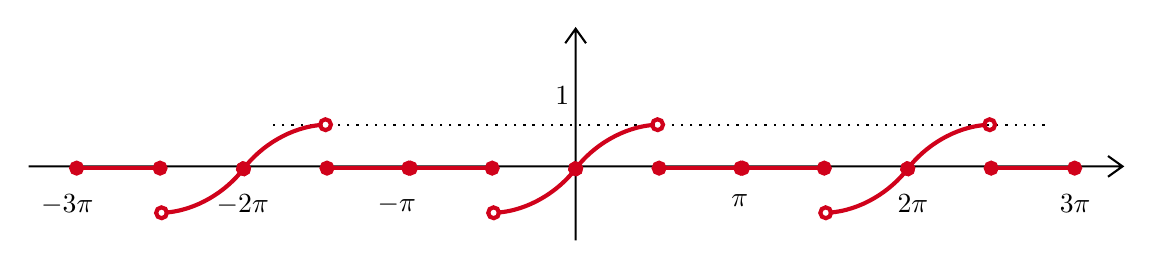
\begin{tikzpicture}[x=0.75pt,y=0.75pt,yscale=-1,xscale=1]
%uncomment if require: \path (0,126); %set diagram left start at 0, and has height of 126

%Straight Lines [id:da10741259255713742] 
\draw  [dash pattern={on 0.84pt off 2.51pt}]  (526.5,59.75) -- (153,59.75) ;
%Shape: Axis 2D [id:dp7770976156065474] 
\draw  (37,79.83) -- (564,79.83)(300.5,13.5) -- (300.5,115.53) (557,74.83) -- (564,79.83) -- (557,84.83) (295.5,20.5) -- (300.5,13.5) -- (305.5,20.5)  ;
%Straight Lines [id:da9173549601591173] 
\draw [color={rgb, 255:red, 208; green, 2; blue, 27 }  ,draw opacity=1 ][line width=1.5]    (380.92,80.67) -- (340.71,80.67) ;
\draw [shift={(340.71,80.67)}, rotate = 180] [color={rgb, 255:red, 208; green, 2; blue, 27 }  ,draw opacity=1 ][fill={rgb, 255:red, 208; green, 2; blue, 27 }  ,fill opacity=1 ][line width=1.5]      (0, 0) circle [x radius= 2.61, y radius= 2.61]   ;
\draw [shift={(380.92,80.67)}, rotate = 180] [color={rgb, 255:red, 208; green, 2; blue, 27 }  ,draw opacity=1 ][fill={rgb, 255:red, 208; green, 2; blue, 27 }  ,fill opacity=1 ][line width=1.5]      (0, 0) circle [x radius= 2.61, y radius= 2.61]   ;
%Curve Lines [id:da4725268586811755] 
\draw [color={rgb, 255:red, 208; green, 2; blue, 27 }  ,draw opacity=1 ][line width=1.5]    (300.5,80.97) .. controls (308.75,70.09) and (323.11,60.82) .. (338.56,59.82) ;
\draw [shift={(340,59.75)}, rotate = 358.21] [color={rgb, 255:red, 208; green, 2; blue, 27 }  ,draw opacity=1 ][line width=1.5]      (0, 0) circle [x radius= 2.61, y radius= 2.61]   ;
\draw [shift={(300.5,80.97)}, rotate = 307.15] [color={rgb, 255:red, 208; green, 2; blue, 27 }  ,draw opacity=1 ][fill={rgb, 255:red, 208; green, 2; blue, 27 }  ,fill opacity=1 ][line width=1.5]      (0, 0) circle [x radius= 2.61, y radius= 2.61]   ;
%Straight Lines [id:da4808528317246443] 
\draw [color={rgb, 255:red, 208; green, 2; blue, 27 }  ,draw opacity=1 ][line width=1.5]    (260.29,80.67) -- (220.08,80.67) ;
\draw [shift={(220.08,80.67)}, rotate = 180] [color={rgb, 255:red, 208; green, 2; blue, 27 }  ,draw opacity=1 ][fill={rgb, 255:red, 208; green, 2; blue, 27 }  ,fill opacity=1 ][line width=1.5]      (0, 0) circle [x radius= 2.61, y radius= 2.61]   ;
\draw [shift={(260.29,80.67)}, rotate = 180] [color={rgb, 255:red, 208; green, 2; blue, 27 }  ,draw opacity=1 ][fill={rgb, 255:red, 208; green, 2; blue, 27 }  ,fill opacity=1 ][line width=1.5]      (0, 0) circle [x radius= 2.61, y radius= 2.61]   ;
%Curve Lines [id:da8687455493649499] 
\draw [color={rgb, 255:red, 208; green, 2; blue, 27 }  ,draw opacity=1 ][line width=1.5]    (300.5,80.97) .. controls (292.26,91.85) and (277.89,101.11) .. (262.44,102.12) ;
\draw [shift={(261,102.18)}, rotate = 178.21] [color={rgb, 255:red, 208; green, 2; blue, 27 }  ,draw opacity=1 ][line width=1.5]      (0, 0) circle [x radius= 2.61, y radius= 2.61]   ;
\draw [shift={(300.5,80.97)}, rotate = 127.15] [color={rgb, 255:red, 208; green, 2; blue, 27 }  ,draw opacity=1 ][fill={rgb, 255:red, 208; green, 2; blue, 27 }  ,fill opacity=1 ][line width=1.5]      (0, 0) circle [x radius= 2.61, y radius= 2.61]   ;

%Straight Lines [id:da599685016533257] 
\draw [color={rgb, 255:red, 208; green, 2; blue, 27 }  ,draw opacity=1 ][line width=1.5]    (540.92,80.67) -- (500.71,80.67) ;
\draw [shift={(500.71,80.67)}, rotate = 180] [color={rgb, 255:red, 208; green, 2; blue, 27 }  ,draw opacity=1 ][fill={rgb, 255:red, 208; green, 2; blue, 27 }  ,fill opacity=1 ][line width=1.5]      (0, 0) circle [x radius= 2.61, y radius= 2.61]   ;
\draw [shift={(540.92,80.67)}, rotate = 180] [color={rgb, 255:red, 208; green, 2; blue, 27 }  ,draw opacity=1 ][fill={rgb, 255:red, 208; green, 2; blue, 27 }  ,fill opacity=1 ][line width=1.5]      (0, 0) circle [x radius= 2.61, y radius= 2.61]   ;
%Curve Lines [id:da4402562566796744] 
\draw [color={rgb, 255:red, 208; green, 2; blue, 27 }  ,draw opacity=1 ][line width=1.5]    (460.5,80.97) .. controls (468.75,70.09) and (483.11,60.82) .. (498.56,59.82) ;
\draw [shift={(500,59.75)}, rotate = 358.21] [color={rgb, 255:red, 208; green, 2; blue, 27 }  ,draw opacity=1 ][line width=1.5]      (0, 0) circle [x radius= 2.61, y radius= 2.61]   ;
\draw [shift={(460.5,80.97)}, rotate = 307.15] [color={rgb, 255:red, 208; green, 2; blue, 27 }  ,draw opacity=1 ][fill={rgb, 255:red, 208; green, 2; blue, 27 }  ,fill opacity=1 ][line width=1.5]      (0, 0) circle [x radius= 2.61, y radius= 2.61]   ;
%Straight Lines [id:da08510756351773896] 
\draw [color={rgb, 255:red, 208; green, 2; blue, 27 }  ,draw opacity=1 ][line width=1.5]    (420.29,80.67) -- (380.08,80.67) ;
\draw [shift={(380.08,80.67)}, rotate = 180] [color={rgb, 255:red, 208; green, 2; blue, 27 }  ,draw opacity=1 ][fill={rgb, 255:red, 208; green, 2; blue, 27 }  ,fill opacity=1 ][line width=1.5]      (0, 0) circle [x radius= 2.61, y radius= 2.61]   ;
\draw [shift={(420.29,80.67)}, rotate = 180] [color={rgb, 255:red, 208; green, 2; blue, 27 }  ,draw opacity=1 ][fill={rgb, 255:red, 208; green, 2; blue, 27 }  ,fill opacity=1 ][line width=1.5]      (0, 0) circle [x radius= 2.61, y radius= 2.61]   ;
%Curve Lines [id:da9678260771297018] 
\draw [color={rgb, 255:red, 208; green, 2; blue, 27 }  ,draw opacity=1 ][line width=1.5]    (460.5,80.97) .. controls (452.26,91.85) and (437.89,101.11) .. (422.44,102.12) ;
\draw [shift={(421,102.18)}, rotate = 178.21] [color={rgb, 255:red, 208; green, 2; blue, 27 }  ,draw opacity=1 ][line width=1.5]      (0, 0) circle [x radius= 2.61, y radius= 2.61]   ;
\draw [shift={(460.5,80.97)}, rotate = 127.15] [color={rgb, 255:red, 208; green, 2; blue, 27 }  ,draw opacity=1 ][fill={rgb, 255:red, 208; green, 2; blue, 27 }  ,fill opacity=1 ][line width=1.5]      (0, 0) circle [x radius= 2.61, y radius= 2.61]   ;

%Straight Lines [id:da6685458363363093] 
\draw [color={rgb, 255:red, 208; green, 2; blue, 27 }  ,draw opacity=1 ][line width=1.5]    (220.92,80.67) -- (180.71,80.67) ;
\draw [shift={(180.71,80.67)}, rotate = 180] [color={rgb, 255:red, 208; green, 2; blue, 27 }  ,draw opacity=1 ][fill={rgb, 255:red, 208; green, 2; blue, 27 }  ,fill opacity=1 ][line width=1.5]      (0, 0) circle [x radius= 2.61, y radius= 2.61]   ;
\draw [shift={(220.92,80.67)}, rotate = 180] [color={rgb, 255:red, 208; green, 2; blue, 27 }  ,draw opacity=1 ][fill={rgb, 255:red, 208; green, 2; blue, 27 }  ,fill opacity=1 ][line width=1.5]      (0, 0) circle [x radius= 2.61, y radius= 2.61]   ;
%Curve Lines [id:da31702343634185315] 
\draw [color={rgb, 255:red, 208; green, 2; blue, 27 }  ,draw opacity=1 ][line width=1.5]    (140.5,80.97) .. controls (148.75,70.09) and (163.11,60.82) .. (178.56,59.82) ;
\draw [shift={(180,59.75)}, rotate = 358.21] [color={rgb, 255:red, 208; green, 2; blue, 27 }  ,draw opacity=1 ][line width=1.5]      (0, 0) circle [x radius= 2.61, y radius= 2.61]   ;
\draw [shift={(140.5,80.97)}, rotate = 307.15] [color={rgb, 255:red, 208; green, 2; blue, 27 }  ,draw opacity=1 ][fill={rgb, 255:red, 208; green, 2; blue, 27 }  ,fill opacity=1 ][line width=1.5]      (0, 0) circle [x radius= 2.61, y radius= 2.61]   ;
%Straight Lines [id:da9353356461505657] 
\draw [color={rgb, 255:red, 208; green, 2; blue, 27 }  ,draw opacity=1 ][line width=1.5]    (100.29,80.67) -- (60.08,80.67) ;
\draw [shift={(60.08,80.67)}, rotate = 180] [color={rgb, 255:red, 208; green, 2; blue, 27 }  ,draw opacity=1 ][fill={rgb, 255:red, 208; green, 2; blue, 27 }  ,fill opacity=1 ][line width=1.5]      (0, 0) circle [x radius= 2.61, y radius= 2.61]   ;
\draw [shift={(100.29,80.67)}, rotate = 180] [color={rgb, 255:red, 208; green, 2; blue, 27 }  ,draw opacity=1 ][fill={rgb, 255:red, 208; green, 2; blue, 27 }  ,fill opacity=1 ][line width=1.5]      (0, 0) circle [x radius= 2.61, y radius= 2.61]   ;
%Curve Lines [id:da990279944542586] 
\draw [color={rgb, 255:red, 208; green, 2; blue, 27 }  ,draw opacity=1 ][line width=1.5]    (140.5,80.97) .. controls (132.26,91.85) and (117.89,101.11) .. (102.44,102.12) ;
\draw [shift={(101,102.18)}, rotate = 178.21] [color={rgb, 255:red, 208; green, 2; blue, 27 }  ,draw opacity=1 ][line width=1.5]      (0, 0) circle [x radius= 2.61, y radius= 2.61]   ;
\draw [shift={(140.5,80.97)}, rotate = 127.15] [color={rgb, 255:red, 208; green, 2; blue, 27 }  ,draw opacity=1 ][fill={rgb, 255:red, 208; green, 2; blue, 27 }  ,fill opacity=1 ][line width=1.5]      (0, 0) circle [x radius= 2.61, y radius= 2.61]   ;


% Text Node
\draw (41.5,92.13) node [anchor=north west][inner sep=0.75pt]  [font=\normalsize]  {$-3\pi $};
% Text Node
\draw (126.07,92.13) node [anchor=north west][inner sep=0.75pt]  [font=\normalsize]  {$-2\pi $};
% Text Node
\draw (203.6,92.13) node [anchor=north west][inner sep=0.75pt]  [font=\normalsize]  {$-\pi $};
% Text Node
\draw (374.04,92.13) node [anchor=north west][inner sep=0.75pt]  [font=\normalsize]  {$\pi $};
% Text Node
\draw (454.1,92.13) node [anchor=north west][inner sep=0.75pt]  [font=\normalsize]  {$2\pi $};
% Text Node
\draw (532.3,92.13) node [anchor=north west][inner sep=0.75pt]  [font=\normalsize]  {$3\pi $};
% Text Node
\draw (289.25,39.76) node [anchor=north west][inner sep=0.75pt]  [font=\normalsize]  {$1$};


\end{tikzpicture}
\end{figure}
\FloatBarrier

\item Poiché

\begin{equation*}
\int ^{\pi }_{-\pi } f^{2}( x) dx< +\infty \ \ \Rightarrow \ \ f\in L^{2}([ -\pi ,\pi ])
\end{equation*}

allora la serie di Fourier converge in media quadratica.
\item $f$ è una funzione regolare a tratti in $[ -\pi ,\pi ]$, allora converge puntualmente $\forall x\in \mathbb{R}$.

Più precisamente converge puntualmente a $f( x) ,\ \forall x\neq ( 2k+1)\frac{\pi }{2} ,\ k\in \mathbb{Z}$, mentre converge a $\frac{1}{2} ,\ \forall x=( 2k+1)\frac{\pi }{2} ,\ k\in \mathbb{Z}$.
\item Non c'è convergenza uniforme perché $f$ non è continua su $\mathbb{R}$.
\item $f$ è dispari, allora $a_{n} =0,\ \forall n\in \mathbb{N}$.

\begin{equation*}
\begin{aligned}
b_{n} & =\frac{2}{\pi }\int ^{\pi }_{0} f( x)\sin( nx) dx\\
 & =\frac{2}{\pi }\int ^{\frac{\pi }{2}}_{0} f( x)\sin( nx) dx=\frac{2}{\pi }\int ^{\frac{\pi }{2}}_{0}\sin x\sin( nx) dx
\end{aligned}
\end{equation*}

Possiamo fare un integrale ciclico o usare le formule di Werner. Usiamo il primo\begin{align*}
\frac{2}{\pi }\int ^{\frac{\pi }{2}}_{0}\sin x\sin( nx) dx & \overset{\text{ipp}}{=}\frac{2}{\pi }\left\{\cancel{[ -\cos x\sin( nx)]^{\frac{\pi }{2}}_{0}} +n\int ^{\frac{\pi }{2}}_{0}\cos x\cos( nx) dx\right\}\\
 & =\frac{2n}{\pi }\int ^{\frac{\pi }{2}}_{0}\cos x\cos( nx) dx\\
 & \overset{\text{ipp}}{=}\frac{2n}{\pi }\left\{[\sin x\cos( nx)]^{\frac{\pi }{2}}_{0} +n\int ^{\frac{\pi }{2}}_{0}\sin x\sin( nx) dx\right\}\\
 & =\frac{2n}{\pi }\cos\left( n\frac{\pi }{2}\right) +\frac{2n^{2}}{\pi }\int ^{\frac{\pi }{2}}_{0}\sin x\sin( nx) dx\\
 & \\
\Rightarrow \ \ b_{n} & =\frac{2n}{\pi }\cos\left( n\frac{\pi }{2}\right) +n^{2} b_{n}\\
\left( 1-n^{2}\right) b_{n} & =\frac{2n}{\pi }\cos\left( n\frac{\pi }{2}\right)
\end{align*}

per $n\neq 1$\begin{equation*}
b_{n} =\frac{2}{\pi }\frac{n}{1-n^{2}}\cos\left( n\frac{\pi }{2}\right) =\begin{cases}
( -1)^{\frac{n}{2}}\frac{2}{\pi }\frac{n}{1-n^{2}} , & n\ \text{pari}\\
0, & n\ \text{dispari}
\end{cases}
\end{equation*}

per $n=1$\begin{equation*}
\begin{aligned}
b_{1} & =\frac{2}{\pi }\int ^{\pi }_{0} f( x)\sin( x) dx=\frac{2}{\pi }\int ^{\frac{\pi }{2}}_{0}\sin^{2}( x) dx=\frac{2}{\pi }\int ^{\frac{\pi }{2}}_{0}\frac{1-\cos 2x}{2} dx\\
 & =\frac{1}{\pi }\left[ x-\frac{1}{2}\sin( 2x)\right]^{\frac{\pi }{2}}_{0} =\frac{1}{\pi }\left[\frac{\pi }{2} -0+0-0\right] =\frac{1}{2}
\end{aligned}
\end{equation*}

Allora $( n=2k,\ k\in \mathbb{N})$:

\begin{equation*}
F( x) =\frac{1}{2}\sin x+\frac{2}{\pi }\sum ^{+\infty }_{k=1}( -1)^{k}\frac{2k}{1-4k^{2}}\sin( 2kx)
\end{equation*}
\item In $x=\frac{\pi }{4}$ la $f$ è continua, quindi la $F( x)$ converge puntualmente a $f( x)$.\begin{align*}
F\left(\frac{\pi }{4}\right) & =\sin\left(\frac{\pi }{4}\right) =\frac{1}{\sqrt{2}}\\
F\left(\frac{\pi }{4}\right) & =\frac{1}{2}\sin\left(\frac{\pi }{4}\right) +\frac{4}{\pi }\sum ^{+\infty }_{k=1}( -1)^{k-1}\frac{k}{4k^{2} -1}\sin\left( k\frac{\pi }{2}\right)\\
\Rightarrow \ \ \frac{1}{\sqrt{2}} & =\frac{1}{2\sqrt{2}} +\frac{4}{\pi }\sum ^{+\infty }_{k=0}( -1)^{k-1}\frac{k}{4k^{2} -1}\sin\left( k\frac{\pi }{2}\right)
\end{align*}

Notiamo che la serie si annulla ogni volta che $k$ è pari, essendo il seno di $\pi ,2\pi ,3\pi \dotsc $, quindi possiamo sommare direttamente sui dispari

\begin{equation*}
\begin{aligned}
\frac{1}{\sqrt{2}} & =\frac{1}{2\sqrt{2}} +\frac{4}{\pi }\sum ^{+\infty }_{k=0}\cancel{( -1)^{( 2k+1) -1}}\frac{2k+1}{4( 2k+1)^{2} -1}\underbrace{\sin\left(( 2k+1)\frac{\pi }{2}\right)}_{( -1)^{k}}\\
\frac{1}{2\sqrt{2}} & =\frac{4}{\pi }\sum ^{+\infty }_{k=0}\frac{2k+1}{4( 2k+1)^{2} -1}( -1)^{k}\\
 & \Rightarrow \ \ \sum ^{+\infty }_{k=0}\frac{2k+1}{4( 2k+1)^{2} -1}( -1)^{k} =\frac{\pi }{8\sqrt{2}}
\end{aligned}
\end{equation*}
\item $f\in L^{2}([ -\pi ,\pi ])$ allora vale l'identità di Parseval

\begin{equation*}
\frac{1}{\pi }\int ^{\pi }_{-\pi }| f( x)| ^{2} dx=\frac{a^{2}_{0}}{2} +\sum\limits ^{\infty }_{n=1}\left( a^{2}_{n} +b^{2}_{n}\right)
\end{equation*}

Nel nostro caso $f$ è dispari, $a_{n} =0,\ \forall n\in \mathbb{N}$, e si ha

\begin{equation*}
\underbrace{\frac{1}{\pi }\int ^{\pi }_{-\pi }| f( x)| ^{2} dx}_{A} =\underbrace{\sum\limits ^{\infty }_{n=1} b^{2}_{n}}_{B}
\end{equation*}

Termine $A$\begin{equation*}
\begin{aligned}
\frac{1}{\pi }\int ^{\pi }_{-\pi }| f( x)| ^{2} dx & =\frac{1}{\pi }\int ^{\frac{\pi }{2}}_{-\frac{\pi }{2}}\sin^{2}( x) dx=\frac{1}{\pi }\int ^{\frac{\pi }{2}}_{-\frac{\pi }{2}}\frac{1-\cos( 2x)}{2} dx\\
 & =\frac{1}{2\pi }\left[ x-\frac{1}{2}\sin( 2x)\right]^{\pi /2}_{-\pi /2} =\frac{1}{2\pi }\left[\frac{\pi }{2} +\frac{\pi }{2}\right] =\frac{1}{2}
\end{aligned}
\end{equation*}

Termine $B$\begin{equation*}
\begin{aligned}
\sum\limits ^{\infty }_{n=1} b^{2}_{n} & =b^{2}_{1} +\sum\limits ^{\infty }_{n=1} b^{2}_{2n}\\
 & =\left(\frac{1}{2}\right)^{2} +\frac{4}{\pi ^{2}}\sum\limits ^{\infty }_{n=1}\frac{4n^{2}}{\left( 4n^{2} -1\right)^{2}}
\end{aligned}
\end{equation*}

Ugualiamo i termini

\begin{equation*}
\frac{1}{2} =\frac{1}{4} +\frac{4}{\pi ^{2}}\sum\limits ^{\infty }_{n=1}\frac{4n^{2}}{\left( 4n^{2} -1\right)^{2}} \ \ \Rightarrow \ \ \sum\limits ^{\infty }_{n=1}\frac{4n^{2}}{\left( 4n^{2} -1\right)^{2}} =\frac{\pi ^{2}}{64}
\end{equation*}
\end{enumerate}
\Soluzione

Notiamo che sono serie convergenti, perché asintotiche a $\frac{1}{n^{\alpha }}$ con $\alpha  >1$.

$f$ è pari, allora $b_{n} =0,\ \forall n\geqslant 1$.
\begin{align*}
a_{0} & =\frac{2}{\pi }\int ^{\pi }_{0} xdx=\frac{2}{\pi }\frac{\pi ^{2}}{2} =\pi \\
 & \\
a_{n} & \overset{n\geqslant 1}{=}\frac{1}{\pi }\int ^{\pi }_{-\pi } f( x)\cos( nx) dx=\frac{2}{\pi }\int ^{\pi }_{0} x\cos( nx) dx\\
 & \overset{\text{ipp}}{=}\frac{2}{\pi }\left\{\cancel{\left[\frac{x\sin( nx)}{n}\right]^{\pi }_{0}} -\frac{1}{n}\int ^{\pi }_{0}\sin( nx) dx\right\}\\
 & =-\frac{2}{\pi n}\left[ -\frac{\cos( nx)}{n}\right]^{\pi }_{0} =\frac{2}{\pi n^{2}}\left[( -1)^{n} -1\right] =\begin{cases}
0, & n\ \text{pari}\\
-\frac{4}{\pi n^{2}} , & n\ \text{dispari}
\end{cases}
\end{align*}
Allora
\begin{equation*}
F( x) =\frac{\pi }{2} -\frac{4}{\pi }\sum\limits ^{\infty }_{n=0}\frac{\cos[( 2n+1) x]}{( 2n+1)^{2}}
\end{equation*}
$f\in L^{2}( Q) \Rightarrow $ vale l'identità di Parseval
\begin{equation*}
\underbrace{\frac{1}{\pi }\int ^{\pi }_{-\pi }| f( x)| ^{2} dx}_{A} =\underbrace{\frac{a^{2}_{0}}{2} +\sum\limits ^{\infty }_{n=1}\left( a^{2}_{n} +b^{2}_{n}\right)}_{B}
\end{equation*}
Termine $A$
\begin{equation*}
A=\frac{1}{\pi }\int ^{\pi }_{-\pi } x^{2} dx=\frac{1}{\pi }\left[\frac{x^{3}}{3}\right]^{\pi }_{-\pi } =\frac{1}{\pi }\left\{\frac{\pi ^{3}}{3} +\frac{\pi ^{3}}{3}\right\} =\frac{2\pi ^{2}}{3}
\end{equation*}
Termine $B$
\begin{equation*}
B=\frac{a^{2}_{0}}{2} +\sum\limits ^{\infty }_{n=1}\left( a^{2}_{n} +\cancel{b^{2}_{n}}\right) =\frac{\pi ^{2}}{2} +\frac{16}{\pi ^{2}}\sum\limits ^{\infty }_{\textcolor[rgb]{0.82,0.01,0.11}{n=0}}\frac{1}{( 2n+1)^{4}}
\end{equation*}
Uguagliamo
\begin{equation*}
\frac{2\pi ^{2}}{3} -\frac{\pi ^{2}}{2} =\frac{16}{\pi ^{2}}\sum\limits ^{\infty }_{n=0}\frac{1}{( 2n+1)^{4}} \ \ \Rightarrow \ \ \sum\limits ^{\infty }_{n=0}\frac{1}{( 2n+1)^{4}} =\frac{\pi ^{4}}{96}
\end{equation*}
Osserviamo che
\begin{equation*}
\underbrace{\sum\limits ^{\infty }_{n=0}\frac{1}{( 2n+1)^{4}}}_{\text{sui dispari}} =\underbrace{\sum\limits ^{\infty }_{n=1}\frac{1}{n^{4}}}_{\text{su tutti}} -\underbrace{\sum\limits ^{\infty }_{n=1}\frac{1}{( 2n)^{4}}}_{\text{sui pari}} =\sum\limits ^{\infty }_{n=1}\frac{1}{n^{4}} -\frac{1}{2^{4}}\sum\limits ^{\infty }_{n=1}\frac{1}{n^{4}} =\left( 1-\frac{1}{2^{4}}\right)\sum\limits ^{\infty }_{n=1}\frac{1}{n^{4}}
\end{equation*}
allora
\begin{equation*}
\sum\limits ^{\infty }_{n=1}\frac{1}{n^{4}} =\frac{\sum\limits ^{\infty }_{n=0}\frac{1}{( 2n+1)^{4}}}{1-\frac{1}{2^{4}}} =\frac{\frac{\pi ^{4}}{96}}{1-\frac{1}{2^{4}}} =\frac{\pi ^{4}}{90}
\end{equation*}
\Soluzione

La funzione è dispari, per cui $a_{n} =0,\forall n$.
\begin{align*}
b_{n} & =\frac{1}{\pi }\int ^{\pi }_{-\pi } f( x)\sin( nx) dx\\
 & =\frac{2}{\pi }\int ^{\pi }_{0} f( x)\sin( nx) dx\\
 & =\frac{2}{\pi }\int ^{\pi }_{0}\left( -x^{2} +x\pi \right)\sin( nx) dx\\
 & =\frac{2}{\pi }\left\{\cancel{\left[\left( -x^{2} +x\pi \right) \cdotp \left( -\frac{\cos( nx)}{n}\right)\right]^{\pi }_{0}} +\frac{1}{n}\int ^{\pi }_{0}\cos( nx)( \pi -2x) dx\right\}\\
 & =\frac{2}{\pi n}\left\{\cancel{\left[( \pi -2x) \cdotp \frac{\sin( nx)}{n}\right]^{\pi }_{0}} +2\int ^{\pi }_{0}\frac{\sin( nx)}{n} dx\right\}\\
 & =\frac{4}{\pi n^{2}}\left\{\int ^{\pi }_{0}\sin( nx) dx\right\}\\
 & =\frac{4}{\pi n^{2}}\left[ -\frac{\cos( nx)}{n}\right]^{\pi }_{0}\\
 & =\frac{4}{\pi n^{3}}[ 1-\cos( n\pi )]\\
 & =\frac{4}{\pi n^{3}}\left[ 1-( -1)^{n}\right] =\begin{cases}
\frac{8}{\pi n^{3}} , & n\ \text{dispari}\\
0, & n\ \text{pari}
\end{cases}
\end{align*}
La serie di Fourier cercata è
\begin{align*}
F( x) & =\sum\limits ^{\infty }_{n=1} b_{n}\sin( nx)\\
 & =\sum\limits ^{\infty }_{n=1}\frac{4}{\pi n^{3}}\left[ 1-( -1)^{n}\right]\sin( nx)\\
 & =\sum\limits ^{\infty }_{n=0}\frac{8}{\pi ( 2n+1)^{3}}\sin(( 2n+1) x)
\end{align*}
Scriviamo l'identità di Parseval
\begin{align*}
\frac{1}{\pi }\int ^{\pi }_{-\pi }[ f( x)]^{2} dx & =\cancel{\frac{a^{2}_{0}}{2}} +\sum\limits ^{\infty }_{n=1}\left(\cancel{a^{2}_{n}} +b^{2}_{n}\right)\\
\frac{1}{\pi } \cdotp 2\int ^{\pi }_{0}\left( x\pi -x^{2}\right)^{2} dx & =\sum\limits ^{\infty }_{n=1} b^{2}_{n}\\
\frac{2}{\pi }\int ^{\pi }_{0}\left[ x^{4} +x^{2} \pi ^{2} -2\pi x^{3}\right) dx & =\sum\limits ^{\infty }_{n=0}\frac{8^{2}}{\pi ^{2}( 2n+1)^{6}}\\
\frac{2}{\pi }\left[\frac{\pi ^{5}}{5} +\frac{\pi ^{3}}{3} \pi ^{2} -2\pi \frac{\pi ^{4}}{4}\right] & =\sum\limits ^{\infty }_{n=0}\frac{64}{\pi ^{2}( 2n+1)^{6}}\\
\frac{\pi ^{4}}{15} & =\frac{64}{\pi ^{2}}\sum\limits ^{\infty }_{n=0}\frac{1}{( 2n+1)^{6}}\\
 & \Rightarrow \ \ \sum\limits ^{\infty }_{n=0}\frac{1}{( 2n+1)^{6}} =\frac{\pi ^{6}}{960}
\end{align*}
Per il secondo risultato sappiamo che la somma su tutti i naturali è come sommare tutti i dispari e tutti i pari. Chiamiamo $J$ la serie cercata
\begin{align*}
\sum\limits ^{\infty }_{n=1}\frac{1}{n^{6}} & =\sum\limits ^{\infty }_{n=0}\frac{1}{( 2n+1)^{6}} +\sum\limits ^{\infty }_{n=1}\frac{1}{( 2n)^{6}}\\
J & =\frac{\pi ^{6}}{960} +\frac{1}{2^{6}} J\\
 & \Rightarrow \ \ J=\frac{\frac{\pi ^{6}}{960}}{1-\frac{1}{2^{6}}} =\frac{\pi ^{6}}{945}
\end{align*}
\Soluzione

Disegnamo il grafico di
\begin{equation*}
f_{n}( x) =\begin{cases}
ne^{n( x-1)} , & x\leqslant 1\\
0, & x >1
\end{cases}
\end{equation*}
\fg{0.7}{12-4}
\begin{enumerate}
\item Fissiamo $x_{0} \in \mathbb{R}$
\begin{enumerate}
\item Se $x_{0} =1\Rightarrow f_{n}( 1) =n\xrightarrow{n\rightarrow +\infty } +\infty $.
\item Se $x_{0} \neq 1\Rightarrow f_{n}( x_{0})\xrightarrow{n\rightarrow +\infty } 0$.
\end{enumerate}

Quindi converge puntualmente alla funzione limite $f( x) \equiv 0\ \forall x\neq 1$.
\item $\forall \varphi \in D(\mathbb{R})$, cioè per ogni $\varphi $ a supporto compatto in $\mathbb{R}$,\begin{align*}
\langle f_{n} ,\varphi \rangle  & =\int _{\mathbb{R}} f_{n}( x) \varphi ( x) dx\\
 & =\int ^{1}_{-\infty } ne^{n( x-1)} \varphi ( x) dx\\
 & \overset{\text{ipp}}{=}\left[ e^{n( x-1)} \varphi ( x)\right]^{1}_{-\infty } -\int ^{1}_{-\infty } e^{n( x-1)} \varphi '( x) dx\\
 & =\varphi ( 1) -\int ^{1}_{-\infty } e^{n( x-1)} \varphi '( x) dx
\end{align*}

Obiettivo: calcolare il limite per $n\rightarrow +\infty $\begin{align*}
\lim\limits _{n\rightarrow +\infty } \langle f_{n} ,\varphi \rangle  & =\lim\limits _{n\rightarrow +\infty }\left[ \varphi ( 1) -\int ^{1}_{-\infty } e^{n( x-1)} \varphi '( x) dx\right]\\
 & =\varphi ( 1) -\lim\limits _{n\rightarrow +\infty }\int ^{1}_{-\infty } e^{n( x-1)} \varphi '( x) dx\\
 & \overset{\text{Dom}}{=} \varphi ( 1) -\int ^{1}_{-\infty }\underbrace{\lim\limits _{n\rightarrow +\infty } e^{n( x-1)} \varphi '( x)}_{=0} dx=\varphi ( 1)
\end{align*}

Posso applicare il teorema della convergenza dominata perché $\varphi \in D(\mathbb{R})$. $\exists M$ tale che $| \varphi '( x)| < M,\ \forall x\in \mathbb{R}$.

\begin{equation*}
\left| e^{n( x-1)} \varphi '( x)\right| \leqslant Me^{x-1} \in L^{1}(( -\infty ,1))
\end{equation*}

Quindi concludiamo che

\begin{equation*}
f_{n}\xrightarrow[n\rightarrow +\infty ]{D'(\mathbb{R})} \delta _{1} \ 
\end{equation*}

nel senso delle distribuzioni.
\end{enumerate}
\Soluzione
\begin{enumerate}
\item Studiamo il limite puntuale di

\begin{gather*}
f_{n,\alpha }( x) =n^{\alpha }\sqrt{1-n| x| } \cdotp \chi _{\left[ -\frac{1}{n} ,\frac{1}{n}\right]}( x)\\
\lim\limits _{n\rightarrow +\infty } f_{n,\alpha }( x) =\begin{cases}
+\infty , & x=0\\
0, & x\neq 0
\end{cases} \ \ \Rightarrow \ \ f_{n,\alpha }( x)\xrightarrow{n\rightarrow +\infty } f( x) \equiv 0\ \text{q.o.}
\end{gather*}
\item Calcoliamo il limite della norma elevata alla $p$ della differenza e per quali condizioni tende a zero\begin{align*}
 & \int _{\mathbb{R}}[ f_{n,\alpha }( x) -0]^{p} d\xrightarrow{n\rightarrow +\infty } 0\\
 & \Leftrightarrow \ \ 2\int ^{1/n}_{0} n^{\alpha p}( 1-nx)^{p/2} dx\xrightarrow{n\rightarrow +\infty } 0\\
 & \Leftrightarrow \ \ 2n^{\alpha p}\int ^{1/n}_{0}( 1-nx)^{p/2} dx\xrightarrow{n\rightarrow +\infty } 0\\
 & \Leftrightarrow \ \ 2n^{\alpha p}\left[\frac{( 1-nx)^{p/2+1}}{\frac{p}{2} +1} \cdotp \left(\frac{1}{-n}\right)\right]^{1/n}_{0}\xrightarrow{n\rightarrow +\infty } 0\\
 & \Leftrightarrow \ \ 2n^{\alpha p} \cdotp \frac{1}{n\left(\frac{p}{2} +1\right)}\xrightarrow{n\rightarrow +\infty } 0\\
 & \Leftrightarrow \ \ C\cdotp n^{\alpha p-1}\xrightarrow{n\rightarrow +\infty } 0\\
 & \Leftrightarrow \ \ \alpha p-1< 0\\
 & \Leftrightarrow \ \ \alpha < \frac{1}{p} \land \alpha  >0
\end{align*}

Notiamo infine che le $f_{n,\alpha }$ non sono limitate, quindi\begin{equation*}
f_{n,\alpha }\cancel{\xrightarrow[n\rightarrow +\infty ]{L^{\infty }(\mathbb{R})}} 0
\end{equation*}
\item Per $\alpha =1$

\begin{equation*}
f_{n,1}( x) =n\sqrt{1-n| x| } \cdotp \chi _{\left[ -\frac{1}{n} ,\frac{1}{n}\right]}( x)
\end{equation*}

Per ogni $\varphi \in D(\mathbb{R})$\begin{align*}
\langle f_{n,1} ,\varphi \rangle  & =\int _{\mathbb{R}} f_{n,1}( x) \varphi ( x) dx=n\int ^{\frac{1}{n}}_{-\frac{1}{n}}\sqrt{1-n| x| } \cdotp \varphi ( x) dx\\
 & =n\left\{\int ^{0}_{-\frac{1}{n}}\sqrt{1+nx} \cdotp \varphi ( x) dx+\int ^{\frac{1}{n}}_{0}\sqrt{1-nx} \cdotp \varphi ( x) dx\right\}\\
 & \begin{array}{ c c }
\varphi ( x) & \varphi '( x)\\
\frac{1}{n}\frac{( 1+nx)^{3/2}}{\frac{3}{2}} & \sqrt{1+nx}\\
-\frac{1}{n}\frac{( 1-nx)^{3/2}}{\frac{3}{2}} & \sqrt{1-nx}
\end{array}\\
 & \overset{\text{ipp}}{=} n\left\{\left[\frac{2}{3n}\sqrt{(1+nx)^{3}} \varphi (x)\right]^{0}_{-1/n} -\frac{2}{3n}\int ^{0}_{-\frac{1}{n}}\sqrt{(1+nx)^{3}} \varphi '(x)dx+\right. \\
 & \left. +\left[ -\frac{2}{3n}\sqrt{(1-nx)^{3}} \varphi (x)\right]^{1/n}_{0} +\frac{2}{3n}\int ^{1/n}_{0}\sqrt{(1+nx)^{3}} \varphi '(x)dx\right\}\\
 & =2\cdotp \frac{2}{3} \varphi ( 0) +\frac{2}{3}\left\{-\int ^{0}_{-\frac{1}{n}}\sqrt{(1+nx)^{3}} \varphi '(x)dx+\int ^{1/n}_{0}\sqrt{(1+nx)^{3}} \varphi '(x)dx\right\}
\end{align*}

Quindi

\begin{equation*}
\lim\limits _{n\rightarrow +\infty } \langle f_{n,1} ,\varphi \rangle =\frac{4}{3} \varphi ( 0) +\frac{2}{3}\lim\limits _{n\rightarrow +\infty }\left\{-\int ^{0}_{-\frac{1}{n}} \dotsc dx+\int ^{1/n}_{0} \dotsc dx\right\}
\end{equation*}

A questo punto osserviamo che

\begin{equation*}
\varphi \in D(\mathbb{R}) \ \ \Rightarrow \ \ M=\max_{x\in [ -1,1]} \varphi ( x)
\end{equation*}

Con un ragionamento analogo a prima\begin{equation*}
\Rightarrow \ \ f_{n,1}\xrightarrow[n\rightarrow +\infty ]{D'(\mathbb{R})}\frac{4}{3} \delta _{0}
\end{equation*}
\end{enumerate}
\chapter{Esercitazione 7 - Boella}
\ParteEsercizi
\Esercizio{}

Calcolare la derivata nel senso delle distribuzioni di
\begin{equation*}
f(x)=\arctan\left(\frac{1}{x}\right)
\end{equation*}
\Esercizio{}

Calcolare la derivata prima e seconda nel senso delle distribuzioni in $D'( 0,5)$ di
\begin{equation*}
f(x)=\begin{cases}
x+x^{2} , & 0< x< 2\\
6, & 2< x< 5
\end{cases}
\end{equation*}
\Esercizio{}

Trovare l'equivalente in $D'(\mathbb{R} )$ di
\begin{equation*}
u(x)=x\delta '_{0} (x)
\end{equation*}
\Esercizio{}

Calcolare il limite delle $f_{n}$ in $L^{p} (\mathbb{R} )$, $D'(\mathbb{R} )$ e $\mathcal{S} '(\mathbb{R} )$ di\footnote{Dove $H$ indica la funzione di Heaviside.}
\begin{equation*}
g(x)=H(x)e^{-x} \ \ \ \ f_{n} (x)=g(x)*\chi _{(0,n)}
\end{equation*}
\Esercizio{}

Calcolare la serie di Fourier associata alla funzione $2\pi $-periodica dispari
\begin{equation*}
f(x)=\begin{cases}
1, & 0< x< \pi \\
-1, & -\pi < x< 0
\end{cases}
\end{equation*}
\ParteSoluzioni
\Soluzione

Dato che $f\in L^{1}_{\mathrm{loc}} (\mathbb{R} )\Rightarrow f\in D'(\mathbb{R} )$.

Sappiamo anche che $f\in \mathcal{S} '(\mathbb{R})$, lo spazio delle distribuzioni temperate.

\fg{0.7}{13-1}

Calcolo quindi la derivata nel senso delle distribuzioni. Ricordiamo innanzitutto che
\begin{equation*}
\frac{d}{dx}\arctan\left(\frac{1}{x}\right) =-\frac{1}{1+\left(\frac{1}{x}\right)^{2}}\frac{1}{x^{2}} =-\frac{1}{1+x^{2}}
\end{equation*}
Calcoliamo
\begin{align*}
\langle f',\varphi \rangle  & =-\langle f,\varphi '\rangle =-\int _{\mathbb{R}}\arctan\left(\frac{1}{x}\right) \varphi '(x)dx=\\
 & =-\int ^{0}_{-\infty }\arctan\left(\frac{1}{x}\right) \varphi '(x)dx-\int ^{+\infty }_{0}\arctan\left(\frac{1}{x}\right) \varphi '(x)dx=\\
 & \overset{\text{ipp}}{=} -\left[\arctan\left(\frac{1}{x}\right) \varphi (x)\right]^{0}_{-\infty } +\int ^{+\infty }_{0}\frac{-1}{1+x^{2}} \varphi ( x) dx\\
 & \ \ \ \ \ -\left[\arctan\left(\frac{1}{x}\right) \varphi (x)\right]^{+\infty }_{0} +\int ^{+\infty }_{0}\frac{-1}{1+x^{2}} \varphi ( x) dx\\
 & =\frac{\pi }{2} \varphi ( 0) +\frac{\pi }{2} \varphi ( 0) +\int _{\mathbb{R}}\frac{-1}{1+x^{2}} \varphi (x)dx\\
 & =\pi \langle \delta _{0} ,\varphi \rangle +\langle \frac{-1}{1+x^{2}} ,\varphi \rangle =\langle \pi \delta _{0} -\frac{1}{1+x^{2}} ,\varphi \rangle 
\end{align*}
Quindi
\begin{equation*}
f'(x)\overset{D'}{=} \pi \delta _{0} -\frac{1}{1+x^{2}}
\end{equation*}
che può essere rappresentata come la funzione $1/\left( 1+x^{2}\right)$ con un salto in $x=0$ verso l'alto di ampiezza $\pi $.
\Soluzione

Dato che $f\in L^{1}_{\mathrm{loc}} (0,5)\Rightarrow f\in D'(0,5)$.

\fg{0.7}{13-2}

Questo significa che la funzione $\varphi (x)$ sarà identicamente nulla su qualsiasi intervallo esterno a $(0,5)$, cioé in particolare $\varphi ( 0) =\varphi ( 5) =0$.
\begin{align*}
\langle f',\varphi \rangle  & =-\langle f,\varphi '\rangle =-\int ^{5}_{0} f(x)\varphi '(x)dx\\
 & =-\left\{\int ^{2}_{0} (x+x^{2} )\varphi '(x)dx+\int ^{5}_{2} 6\varphi '(x)dx\right\}\\
 & \overset{\text{ipp}}{=} -\left\{\left[ (x+x^{2} )\varphi (x)\right]^{2}_{0} -\int ^{2}_{0} (1+2x)\varphi (x)dx+[ 6\varphi (x)]^{5}_{2}\right\}\\
 & =-\left\{\cancel{6\varphi ( 2)} -0-\int ^{2}_{0}( 1+2x) \varphi ( x) dx+\cancel{6\varphi ( 5)} -\cancel{6\varphi ( 2)}\right\}\\
 & =\int ^{2}_{0}( 1+2x) \varphi ( x) dx
\end{align*}
Definiamo
\begin{equation*}
g(x)=\begin{cases}
2x+1, & 0< x< 2\\
0, & 2< x< 5
\end{cases} \ \ \Rightarrow \ \ \langle f',\varphi \rangle =\int _{\mathbb{R}} g( x) \varphi ( x) dx=\langle g,\varphi \rangle 
\end{equation*}
ovvero
\begin{equation*}
f'(x)\overset{D'( 0,5)}{=} g(x)
\end{equation*}
Derivata seconda. Si prosegue in maniera analoga:
\begin{equation*}
\begin{aligned}
\langle f'',\varphi \rangle  & =-\langle f',\varphi '\rangle =-\langle g,\varphi '\rangle =-\int ^{2}_{0} (1+2x)\varphi '(x)dx & \\
 & =-\left\{[ (1+2x)\varphi (x)]^{2}_{0} -\int ^{2}_{0} 2\varphi (x)dx\right\} & \\
 & =-\left\{5\varphi (2)-0-\int ^{2}_{0} 2\varphi (x)dx\right\} & h(x)=\begin{cases}
2, & 0< x< 2\\
0, & 2< x< 5
\end{cases}\\
 & \overset{}{=} -5\varphi (2)+\int ^{5}_{0} h(x)\varphi (x)dx & \\
 & =-5\langle \delta _{2} ,\varphi \rangle +\langle h,\varphi \rangle  & \\
 & =\langle h-5\delta _{2} ,\varphi \rangle  & 
\end{aligned}
\end{equation*}
ovvero
\begin{equation*}
f''(x)\overset{D'( 0,5)}{=} h(x)-5\delta _{2}
\end{equation*}
Ciò è coerente con come era stata definita la $g$


\begin{figure}[htpb]
	\centering
\tikzset{every picture/.style={line width=0.75pt}} %set default line width to 0.75pt        

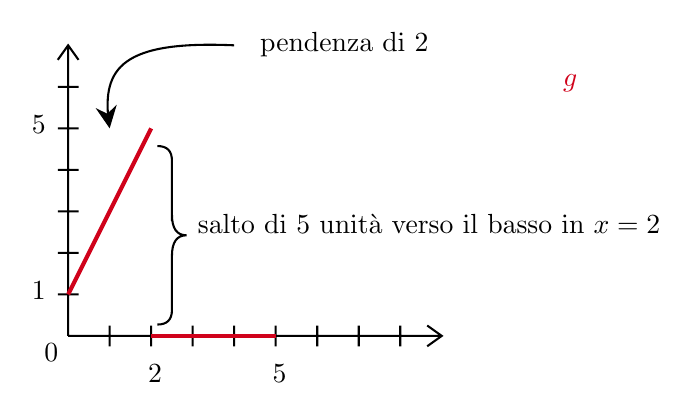
\begin{tikzpicture}[x=0.75pt,y=0.75pt,yscale=-1,xscale=1]
%uncomment if require: \path (0,203); %set diagram left start at 0, and has height of 203

%Shape: Axis 2D [id:dp46013604632113503] 
\draw  (200,160) -- (380,160)(200,20) -- (200,160) -- cycle (373,155) -- (380,160) -- (373,165) (195,27) -- (200,20) -- (205,27) (220,155) -- (220,165)(240,155) -- (240,165)(260,155) -- (260,165)(280,155) -- (280,165)(300,155) -- (300,165)(320,155) -- (320,165)(340,155) -- (340,165)(360,155) -- (360,165)(195,140) -- (205,140)(195,120) -- (205,120)(195,100) -- (205,100)(195,80) -- (205,80)(195,60) -- (205,60)(195,40) -- (205,40) ;
\draw   ;
%Straight Lines [id:da5583914209314376] 
\draw [color={rgb, 255:red, 208; green, 2; blue, 27 }  ,draw opacity=1 ][line width=1.5]    (240,60) -- (200,140) ;
%Straight Lines [id:da8784587512983899] 
\draw [color={rgb, 255:red, 208; green, 2; blue, 27 }  ,draw opacity=1 ][line width=1.5]    (300,160) -- (240,160) ;
%Shape: Brace [id:dp22057370394693132] 
\draw   (243,154.53) .. controls (247.67,154.53) and (250,152.2) .. (250,147.53) -- (250,121.53) .. controls (250,114.86) and (252.33,111.53) .. (257,111.53) .. controls (252.33,111.53) and (250,108.2) .. (250,101.53)(250,104.53) -- (250,75.53) .. controls (250,70.86) and (247.67,68.53) .. (243,68.53) ;
%Curve Lines [id:da9997704212540879] 
\draw    (280,20) .. controls (226.44,17.62) and (216.19,30.57) .. (219.58,57.06) ;
\draw [shift={(220,60)}, rotate = 261.02] [fill={rgb, 255:red, 0; green, 0; blue, 0 }  ][line width=0.08]  [draw opacity=0] (10.72,-5.15) -- (0,0) -- (10.72,5.15) -- (7.12,0) -- cycle    ;

% Text Node
\draw (181,132.4) node [anchor=north west][inner sep=0.75pt]    {$1$};
% Text Node
\draw (181,52.4) node [anchor=north west][inner sep=0.75pt]    {$5$};
% Text Node
\draw (237,172.4) node [anchor=north west][inner sep=0.75pt]    {$2$};
% Text Node
\draw (187,162.4) node [anchor=north west][inner sep=0.75pt]    {$0$};
% Text Node
\draw (297,172.4) node [anchor=north west][inner sep=0.75pt]    {$5$};
% Text Node
\draw (437,32.4) node [anchor=north west][inner sep=0.75pt]  [color={rgb, 255:red, 208; green, 2; blue, 27 }  ,opacity=1 ]  {$g$};
% Text Node
\draw (261,100) node [anchor=north west][inner sep=0.75pt]   [align=left] {salto di $5$ unità verso il basso in $x=2$};
% Text Node
\draw (291,12) node [anchor=north west][inner sep=0.75pt]   [align=left] {pendenza di $2$};


\end{tikzpicture}
\end{figure}
\FloatBarrier

Il salto verso l'alto in $x=0$ non lo possiamo vedere perché le funzioni test sono nulle prima di zero.
\Soluzione
\begin{nb}
Si può dimostrare che se $v\in D'(\mathbb{R})$, $\psi \in C^{\infty }(\mathbb{R}) \Rightarrow \psi v\in D'(\mathbb{R})$ e il suo effetto su una funzione test $\varphi $ è
\begin{equation*}
\langle \psi v,\varphi \rangle :=\langle v,\psi \varphi \rangle 
\end{equation*}
\end{nb}
Quindi
\begin{equation*}
\langle x\delta '_{0} (x),\varphi \rangle =\langle \delta '_{0} (x),x\varphi ( x) \rangle =-\langle \delta _{0} ,x\varphi '( x) +\varphi ( x) \rangle =-\varphi ( 0) =\langle -\delta _{0} ,\varphi \rangle 
\end{equation*}
Cioè in $D'(\mathbb{R})$
\begin{equation*}
x\delta '_{0} =-\delta _{0}
\end{equation*}
\textit{Esercizio per casa.}

$\forall n,m\in \mathbb{N}$ trovare la distribuzione di $u( x) =x^{m} \delta ^{( n)}_{0}$.
\Soluzione
\begin{equation*}
f_{n} (x)=g(x)*\chi _{(0,n)} =\int _{\mathbb{R}} e^{-(x-t)} H(x-t)\chi _{(0,n)} (t)dt=\int ^{n}_{0} e^{-x} e^{t} H(x-t)dt
\end{equation*}
\fg{0.7}{13-3}
\begin{gather*}
\begin{cases}
0, & x< 0\\
\int ^{x}_{0} e^{-x} e^{t} dt, & 0\leqslant x\leqslant n\\
\int ^{n}_{0} e^{-x} e^{t} dt, & x >n
\end{cases} =\begin{cases}
0, & x< 0\\
e^{-x}\left( e^{x} -1\right) =1-e^{-x} & 0\leqslant x\leqslant n\\
e^{-x} (e^{n} -1) & x >n
\end{cases}\\
\\
\xrightarrow{n\rightarrow \infty } F( x) =\begin{cases}
0, & x< 0\\
1-e^{-x} , & x\geqslant 0
\end{cases}
\end{gather*}
\begin{itemize}
\item Convergenza in $L^{p}(\mathbb{R})$?

No perché l'ipotetico limite $F( x)$ non è integrabile a $+\infty $.
\item Convergenza in $L^{\infty }(\mathbb{R})$?

Notiamo che

\begin{equation*}
\begin{aligned}
\Vert F\Vert _{L^{\infty }(\mathbb{R})} & =\sup _{\mathbb{R}}| F( x)| =1\xrightarrow{n\rightarrow +\infty } 1\\
\Vert f_{n}\Vert _{L^{\infty }(\mathbb{R})} & =\sup _{\mathbb{R}}| f_{n}( x)| =1-e^{-n}\xrightarrow{n\rightarrow +\infty } 1
\end{aligned}
\end{equation*}

Tuttavia non possiamo concludere da queste due affermazioni che c'è convergenza in $L^{\infty }$, quello che ci interessa è la \textit{differenza} in norma infinito.

\begin{equation*}
\Vert f_{n} -F\Vert _{L^{\infty }(\mathbb{R})} =\begin{cases}
0, & x< n\\
F( x) -f_{n}( x) , & x\geqslant n
\end{cases} =\begin{cases}
0, & x< n\\
1-e^{n-x} , & x\geqslant n
\end{cases}
\end{equation*}

È un esponenziale traslato di $n$

\begin{equation*}
\Vert f_{n} -F\Vert _{L^{\infty }(\mathbb{R})} =\sup _{\mathbb{R}}| f_{n}( x) -F( x)| =1\nrightarrow 0
\end{equation*}

Quindi non c'è convergenza in $L^{\infty }(\mathbb{R})$.
\item Convergenza in $D'(\mathbb{R})$?

Sono distribuzioni in quanto $f_{n} ,F\in L^{1}_{\mathrm{loc}}(\mathbb{R})$.

\begin{equation*}
\langle f_{n} ,\varphi \rangle \rightarrow \langle F,\varphi \rangle \ \ \forall \varphi \in D(\mathbb{R}) \ \ \Leftrightarrow \ \ \langle F-f_{n} ,\varphi \rangle \rightarrow 0
\end{equation*}

nel nostro caso

\begin{equation*}
\langle F-f_{n} ,\varphi \rangle =\int ^{\infty }_{n}\left( 1-e^{n-x}\right) \varphi (x)dx=0\ \ \forall n\geqslant n_{\varphi }
\end{equation*}

perché $\varphi $ è a supporto compatto, cioè $\forall \varphi \ \exists n_{\varphi } :\varphi ( x) =0,\forall x\geqslant n$. Il dominio di integrazione prima o poi andrà oltre il dominio di $\varphi $, che poi si annullerà.

Quindi

\begin{equation*}
f_{n}\xrightarrow{D'(\mathbb{R} )} F
\end{equation*}
\item Convergenza in $\mathcal{S} '(\mathbb{R} )$?\begin{equation*}
\langle f_{n} ,\psi \rangle \rightarrow \langle F,\psi \rangle \ \ \forall \psi \in S(\mathbb{R}) \ \ \Leftrightarrow \ \ \langle F-f_{n} ,\psi \rangle \rightarrow 0
\end{equation*}

dove $S$ è lo spazio di Schwarz, lo spazio delle funzioni a decrescita rapida\begin{equation*}
\psi \in C^{\infty } \ \ \land \ \ \lim\limits _{x\rightarrow +\infty } x^{n} \psi ( x) =0
\end{equation*}

nel nostro caso

\begin{equation*}
\langle F-f_{n} ,\psi \rangle =\int ^{+\infty }_{n}\left( 1-e^{n-x}\right) \psi ( x) dx=\int ^{+\infty }_{0}\left( 1-e^{n-x}\right) \chi _{( n,+\infty )}( x) \psi ( x) dx
\end{equation*}

Se chiamiamo $h_{n}( x)$ l'integranda

\begin{equation*}
\lim\limits _{n\rightarrow +\infty } h_{n}( x) =0
\end{equation*}

Usiamo la convergenza dominata

\begin{equation*}
| h_{n}( x)| \leqslant | \psi ( x)| \ \ | \psi ( x)| \in L^{1}(\mathbb{R})
\end{equation*}

Allora

\begin{equation*}
\langle F-f_{n} ,\psi \rangle \rightarrow 0
\end{equation*}
\end{itemize}
\Soluzione
\begin{equation*}
f( x) \sim \sum\limits ^{\infty }_{n=1} b_{n}\sin( nx)
\end{equation*}
Calcoliamo i coefficienti
\begin{equation*}
b_{n} =\frac{2}{\pi }\int ^{\pi }_{0} 1\cdotp \sin( nx) dx=\frac{2}{\pi }\left[ -\frac{1}{n}\cos( nx)\right]^{\pi }_{0} =\frac{2}{\pi n}\left( 1-( -1)^{n}\right) =\begin{cases}
\frac{4}{n\pi } , & n\ \text{dispari}\\
0, & n\ \text{pari}
\end{cases}
\end{equation*}
La serie cercata è
\begin{equation*}
f( x) \sim \sum\limits ^{\infty }_{k=0}\frac{4}{( 2k+1) \pi }\sin(( 2k+1) x)
\end{equation*}
Questa funzione è anche una distribuzione? Sì, $f\in L^{1}_{\mathrm{loc}}(\mathbb{R})$.
\begin{equation*}
\langle u,\varphi \rangle =\langle u,\varphi ( x+T) \rangle 
\end{equation*}
In $D'(\mathbb{R})$, a occhio possiamo dedurre la derivata\footnote{Si noti la somiglianza col Pettine di Dirac.}


\begin{figure}[htpb]
	\centering
\tikzset{every picture/.style={line width=0.75pt}} %set default line width to 0.75pt        

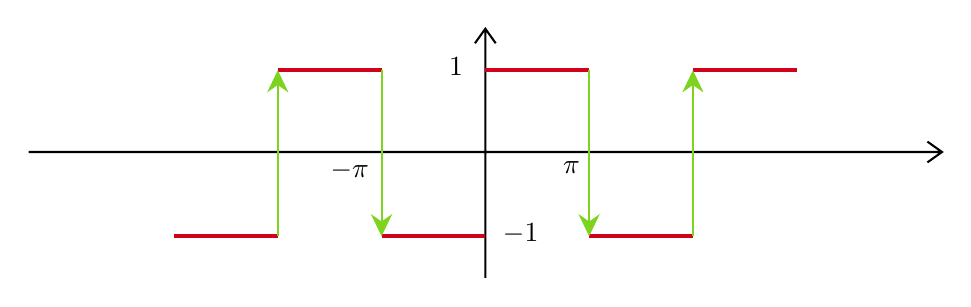
\begin{tikzpicture}[x=0.75pt,y=0.75pt,yscale=-1,xscale=1]
%uncomment if require: \path (0,132); %set diagram left start at 0, and has height of 132

%Shape: Axis 2D [id:dp6130811625741925] 
\draw  (80,69.4) -- (520,69.4)(300,10) -- (300,130) (513,64.4) -- (520,69.4) -- (513,74.4) (295,17) -- (300,10) -- (305,17)  ;
%Straight Lines [id:da4688738915321422] 
\draw [color={rgb, 255:red, 208; green, 2; blue, 27 }  ,draw opacity=1 ][line width=1.5]    (300,30) -- (350,30) ;
%Straight Lines [id:da564644152513289] 
\draw [color={rgb, 255:red, 208; green, 2; blue, 27 }  ,draw opacity=1 ][line width=1.5]    (250,110) -- (300,110) ;
%Straight Lines [id:da1288587788441018] 
\draw [color={rgb, 255:red, 208; green, 2; blue, 27 }  ,draw opacity=1 ][line width=1.5]    (400,30) -- (450,30) ;
%Straight Lines [id:da42001293411482954] 
\draw [color={rgb, 255:red, 208; green, 2; blue, 27 }  ,draw opacity=1 ][line width=1.5]    (350,110) -- (400,110) ;
%Straight Lines [id:da41879142834815575] 
\draw [color={rgb, 255:red, 208; green, 2; blue, 27 }  ,draw opacity=1 ][line width=1.5]    (200,30) -- (250,30) ;
%Straight Lines [id:da34094039721778624] 
\draw [color={rgb, 255:red, 208; green, 2; blue, 27 }  ,draw opacity=1 ][line width=1.5]    (150,110) -- (200,110) ;
%Straight Lines [id:da6751056390959596] 
\draw [color={rgb, 255:red, 126; green, 211; blue, 33 }  ,draw opacity=1 ]   (350,30) -- (350,107) ;
\draw [shift={(350,110)}, rotate = 270] [fill={rgb, 255:red, 126; green, 211; blue, 33 }  ,fill opacity=1 ][line width=0.08]  [draw opacity=0] (10.72,-5.15) -- (0,0) -- (10.72,5.15) -- (7.12,0) -- cycle    ;
%Straight Lines [id:da8152221642203317] 
\draw [color={rgb, 255:red, 126; green, 211; blue, 33 }  ,draw opacity=1 ]   (250,30) -- (250,107) ;
\draw [shift={(250,110)}, rotate = 270] [fill={rgb, 255:red, 126; green, 211; blue, 33 }  ,fill opacity=1 ][line width=0.08]  [draw opacity=0] (10.72,-5.15) -- (0,0) -- (10.72,5.15) -- (7.12,0) -- cycle    ;
%Straight Lines [id:da21495238477473233] 
\draw [color={rgb, 255:red, 126; green, 211; blue, 33 }  ,draw opacity=1 ]   (200,110) -- (200,33) ;
\draw [shift={(200,30)}, rotate = 450] [fill={rgb, 255:red, 126; green, 211; blue, 33 }  ,fill opacity=1 ][line width=0.08]  [draw opacity=0] (10.72,-5.15) -- (0,0) -- (10.72,5.15) -- (7.12,0) -- cycle    ;
%Straight Lines [id:da5779103582115537] 
\draw [color={rgb, 255:red, 126; green, 211; blue, 33 }  ,draw opacity=1 ]   (400,110) -- (400,33) ;
\draw [shift={(400,30)}, rotate = 450] [fill={rgb, 255:red, 126; green, 211; blue, 33 }  ,fill opacity=1 ][line width=0.08]  [draw opacity=0] (10.72,-5.15) -- (0,0) -- (10.72,5.15) -- (7.12,0) -- cycle    ;

% Text Node
\draw (281,22.4) node [anchor=north west][inner sep=0.75pt]    {$1$};
% Text Node
\draw (307,102.4) node [anchor=north west][inner sep=0.75pt]    {$-1$};
% Text Node
\draw (224,72.4) node [anchor=north west][inner sep=0.75pt]    {$-\pi $};
% Text Node
\draw (336,72.4) node [anchor=north west][inner sep=0.75pt]    {$\pi $};


\end{tikzpicture}
\end{figure}
\FloatBarrier

\begin{equation*}
f'( x) =\sum\limits ^{+\infty }_{k=-\infty }( -1)^{k} \cdotp 2\delta _{k\pi }( x)
\end{equation*}
Possiamo derivare termine a termine
\begin{equation*}
f'( x)\overset{D'(\mathbb{R})}{\sim }\sum\limits ^{\infty }_{k=0}\frac{4}{\pi }\cos(( 2k+1) x)
\end{equation*}
\chapter{Esercitazione 7 - Potrich}
\ParteEsercizi
\begin{definition}
[Distribuzione] Una distribuzione è un operatore $u$ che a ogni funzione test $\varphi $ (funzione $C^{\infty }(\mathbb{R})$ il cui supporto è un compatto $\Omega $ contenuto in $\mathbb{R}$) associa un numero, reale o complesso, $\langle u,\varphi \rangle $ chiamato \textbf{dualità} tra $u$ e $\varphi $ tale che:
\begin{equation*}
\begin{array}{ l }
\langle u,a\varphi +b\psi \rangle =a\langle u,\varphi \rangle +b\langle u,\psi \rangle \ \ \forall a,b\in \mathbb{C} ,\ \forall \varphi ,\psi \in D( \Omega )\\
\varphi _{j}\rightarrow \varphi \ \text{in} \ D( \Omega ) \ \ \Rightarrow \ \ \langle u,\varphi _{j} \rangle \rightarrow \langle u,\varphi \rangle 
\end{array}
\end{equation*}
\end{definition}
\begin{obs}
[Delta di Dirac] L'esempio fondamentale di distribuzione in $D'\left(\mathbb{R}^{n}\right)$ è la Delta di Dirac, denotata $\delta $, e così definita
\begin{equation*}
\langle \delta ,\varphi \rangle =\varphi ( 0) \ \ \forall \varphi \in D\left(\mathbb{R}^{n}\right)
\end{equation*}
\end{obs}
\begin{definition}
Se \ $u\in D'(\mathbb{R})$, allora la derivata distribuzionale di $u$ è la distribuzione $u'\in D'(\mathbb{R})$ definita univocamente da
\begin{equation*}
\int _{\mathbb{R}} u'\varphi =-\int _{\mathbb{R}} u\varphi '\ \ \forall \varphi \in D(\mathbb{R})
\end{equation*}
\end{definition}
\begin{definition}
Si definisce prodotto di una distribuzione in $\Omega $ per una funzione $C^{\infty }( \Omega )$: se $\psi \in C^{\infty }( \Omega )$ e $u\in D'(\mathbb{R})$, allora $( \psi u) \in D'( \Omega )$ è la distribuzione tale che
\begin{equation*}
\langle \psi u,\varphi \rangle =\langle u,\psi \varphi \rangle \ \ \forall \varphi \in D\left(\mathbb{R}^{n}\right)
\end{equation*}
\end{definition}
\begin{nb}
\begin{equation*}
\langle u,\varphi \rangle :=\int _{\Omega } u( x) \varphi ( x) dx,\ \ u\in D'( \Omega ) ,\ \varphi \in D( \Omega )
\end{equation*}
\end{nb}
\Esercizio{}

Provare che valgono le seguenti identità in $D'(\mathbb{R})$:
\begin{enumerate}
\item $x\delta ( x) =0$
\item $x\delta '( x) =-\delta ( x)$
\end{enumerate}
\Esercizio{(TDE 6/07/2015)}

Mostrare che, per ogni $n\in \mathbb{N}^{+}$, si ha
\begin{equation*}
\boxed{x^{n} \delta ^{( n)} =( -1)^{n} n!\delta \ \ \text{in} \ D'}
\end{equation*}
\Esercizio{(Teorema di derivazione di funzioni con discontinuità di tipo salto)}

Sia $a\in \mathbb{R}$, $f\in C^{1}(( -\infty ,a))$, $g\in C^{1}(( a,+\infty ))$ con $f'\in L^{1}(( -\infty ,a))$ e $g'\in L^{1}(( a,+\infty ))$ e definiamo
\begin{equation*}
u( x) =\begin{cases}
f( x) , & x< a\\
g( x) , & x >a
\end{cases}
\end{equation*}
allora $u$ risulta definita q.o. su $\mathbb{R}$ e la sua derivata distribuzionale $u'$ è la somma di una funzione localmente integrabile e che coincide con $f'$ in $( -\infty ,a)$ e con $g'$ in $( a,+\infty )$ più una parte singolare, data dalla Delta di Dirac concentrata in $x=a$ e moltiplicata per l'ampiezza del salto
\begin{equation*}
[ u( a_{+}) -u( a_{-})] \delta _{a}
\end{equation*}
\Esercizio{}

Si consideri
\begin{equation*}
f_{n}( x) =\frac{n}{1+n^{2} x^{2}}
\end{equation*}
provare che $f_{n}\rightarrow \pi \delta $ in $\mathcal{S} '(\mathbb{R})$ e in $D'(\mathbb{R})$.
\Esercizio{}

Si considerino
\begin{equation*}
f_{n}( x) =\frac{1}{\sqrt{n}} \chi _{[ 0,n]}( x) \ \ \ \ \ \ \ \ g_{n}( x) =\sin( nx) \chi _{[ 0,7]}( x)
\end{equation*}
Stabilire se le successioni sono convergenti in $L^{1}(\mathbb{R}) ,L^{2}(\mathbb{R}) ,L^{\infty }(\mathbb{R}) ,D'(\mathbb{R}) ,\mathcal{S} '(\mathbb{R})$.
\Esercizio{}

Si consideri
\begin{equation*}
f_{n}( x) =n^{2} xe^{-n| x| }
\end{equation*}
\begin{enumerate}
\item Determinare il limite puntuale
\item Stabilire se $f_{n}$ converge in $L^{p}$, con $p\in [ 1,+\infty ]$
\item Determinare il limite di\begin{equation*}
g_{n}( x) =f_{n}( x) H( x) \ \ \text{in} \ D'(\mathbb{R})
\end{equation*}

dove\begin{equation*}
H( x) =\begin{cases}
1, & x\geqslant 0\\
0, & x< 0
\end{cases}
\end{equation*}

detta \textbf{Funzione di Heaviside}.
\item Determinare il limite di $f_{n}$ in $D'(\mathbb{R})$
\end{enumerate}
\ParteSoluzioni
\Soluzione
\begin{enumerate}
\item $\forall \varphi \in D(\mathbb{R})$\begin{equation*}
\langle x\delta ,\varphi \rangle =\langle \delta ,x\varphi \rangle =0\cdotp \varphi ( 0) =0\qed 
\end{equation*}
\item $\forall \varphi \in D(\mathbb{R})$\begin{gather*}
\begin{aligned}
\langle x\delta ',\varphi \rangle  & =\langle \delta ',x\varphi \rangle =-\langle \delta ,( x\varphi ) '\rangle \\
 & =-\langle \delta ,\varphi +x\varphi '\rangle \\
 & =-\langle \delta ,\varphi \rangle -\langle \delta ,x\varphi '\rangle =-\varphi ( 0)
\end{aligned}\\
\qed 
\end{gather*}
\end{enumerate}
\Soluzione

Per induzione
\begin{itemize}
\item La formula è vera per $n=1$, per l'esercizio precedente\begin{equation*}
x\delta '( x) =-\delta ( x)
\end{equation*}
\item Supponiamo vera la tesi per $n$ generico\begin{equation*}
\langle x^{n} \delta ^{( n)} ,\varphi \rangle =( -1)^{n} n!\langle \delta ,\varphi \rangle \ \ \forall \varphi \in D
\end{equation*}

dobbiamo mostrare che vale anche per $n+1$\begin{gather*}
\begin{aligned}
\langle x^{n+1} \delta ^{( n+1)} ,\varphi \rangle  & =\langle \delta ^{( n+1)} ,x^{n+1} \varphi \rangle =-\langle \delta ^{( n)} ,\left( x^{n+1} \varphi \right) '\rangle \\
 & =-\langle \delta ^{( n)} ,( n+1) x^{n} \varphi +x^{n+1} \varphi '\rangle \\
 & =-\langle x^{n} \delta ^{( n)} ,( n+1) \varphi +x\varphi '\rangle \\
 & \overset{\text{induz.}}{=} -\langle ( -1)^{n} n!\delta ,( n+1) \varphi +x\varphi '\rangle \\
 & =( -1)^{n+1}( n+1) !\langle \delta ,\varphi \rangle \underbrace{-( -1)^{n} n!\langle \delta ,x\varphi '\rangle }_{=0}\\
 & =( -1)^{n+1}( n+1) !\langle \delta ,\varphi \rangle 
\end{aligned}\\
\qed 
\end{gather*}
\end{itemize}
\Soluzione

Per comodità $u( a_{-}) =f( a) :=f( a_{-})$ e $u( a_{+}) =g( a) :=g( a_{+})$.

Questi termini esistono finiti perché $f',g'$ sono integrabili.

$\forall \varphi \in D(\mathbb{R})$
\begin{equation*}
\langle u',\varphi \rangle =-\langle u,\varphi '\rangle =-\int ^{+\infty }_{-\infty } u( x) \varphi '( x) dx
\end{equation*}
la funzione $u$ è definita a tratti
\begin{equation*}
-\int ^{+\infty }_{-\infty } u( x) \varphi '( x) dx=-\int ^{a}_{-\infty } f( x) \varphi '( x) dx-\int ^{+\infty }_{a} g( x) \varphi '( x) dx=( *)
\end{equation*}
integro per parti
\begin{gather*}
\begin{aligned}
( *) & =-[ f( x) \varphi ( x)]^{a}_{-\infty } +\int ^{a}_{-\infty } f'( x) \varphi ( x) dx-[ g( x) \varphi ( x)]^{+\infty }_{a} +\int ^{+\infty }_{a} g'( x) \varphi ( x) dx\\
 & =-f( a) \varphi ( a) +\int ^{a}_{-\infty } f'( x) \varphi ( x) dx+g( a) \varphi ( a) +\int ^{+\infty }_{a} g'( x) \varphi ( x) dx\\
 & =\varphi ( a)[ g( a) -f( a)] +\int ^{a}_{-\infty } f'( x) \varphi ( x) dx+\int ^{+\infty }_{a} g'( x) \varphi ( x) dx\\
 & =[ u( a_{+}) -u( a_{-})] \langle \delta _{x=a} ,\varphi \rangle +\int ^{a}_{-\infty } f'( x) \varphi ( x) dx+\int ^{+\infty }_{a} g'( x) \varphi ( x) dx
\end{aligned}\\
\qed 
\end{gather*}
\textit{Esempio.}
\begin{equation*}
\sgn( x) =\begin{cases}
1, & x >0\\
-1, & x< 0
\end{cases}
\end{equation*}
Per $x >0$, $\sgn '( x) =0$.

Per $x< 0$, $\sgn '( x) =0$.

$\sgn( x)$ presenta un salto in $x=0$ di ampiezza $2$.
\begin{equation*}
\Rightarrow \ \ \sgn '( x) =0+0+2\delta ( x)
\end{equation*}
\textit{Esempio.}
\begin{equation*}
f( x) =\frac{1}{2}\sgn xe^{-| x| } =\begin{cases}
\frac{1}{2} e^{-x} , & x >0\\
-\frac{1}{2} e^{x} , & x< 0
\end{cases}
\end{equation*}
Per $x >0$, $f'( x) =-\frac{1}{2} e^{-x}$.

Per $x< 0$, $f'( x) =-\frac{1}{2} e^{x}$.

$f( x)$ presenta un salto in $x=0$ di ampiezza $1$.
\begin{equation*}
\Rightarrow \ \ f'( x) =-\frac{1}{2} e^{-| x| } +\delta ( x)
\end{equation*}
\Soluzione

\fg{0.45}{14-4}

Se dimostro in $\mathcal{S} '(\mathbb{R})$, quella in $D'(\mathbb{R})$ segue automaticamente.

Devo provare che
\begin{equation*}
\int _{\mathbb{R}}\frac{n\varphi ( x)}{1+n^{2} x^{2}} dx\xrightarrow{n\rightarrow +\infty } \pi \varphi ( 0) \ \ \forall \varphi \in S(\mathbb{R})
\end{equation*}
pongo $nx=t\Rightarrow ndx=dt$
\begin{equation*}
\int _{\mathbb{R}}\frac{n\varphi \left(\frac{t}{n}\right)}{1+t^{2}}\frac{dt}{n} =\int _{\mathbb{R}} \varphi \left(\frac{t}{n}\right)\frac{1}{1+t^{2}} dt
\end{equation*}
Proviamo che tale convergenza ha luogo per ogni $\varphi $ limitata in $0$ stimando la differenza
\begin{equation*}
\left| \int _{\mathbb{R}} \varphi \left(\frac{t}{n}\right)\frac{1}{1+t^{2}} dt-\pi \varphi ( 0)\right| \leqslant \underbrace{\left| \int _{| t| \leqslant T}\frac{\varphi \left(\frac{t}{n}\right) -\varphi ( 0)}{1+t^{2}} dt\right| }_{I_{1}} +\underbrace{\left| \int _{| t|  >T}\frac{\varphi \left(\frac{t}{n}\right) -\varphi ( 0)}{1+t^{2}} dt\right| }_{I_{2}}
\end{equation*}
Per mostrare la convergenza di questi due integrali posso applicare la convergenza dominata
\begin{equation*}
\left| \varphi \left(\frac{t}{n}\right)\frac{1}{1+t^{2}}\right| \leqslant \frac{\Vert \varphi \Vert _{\infty }}{1+t^{2}} \in L^{1}(\mathbb{R})
\end{equation*}
\begin{nb}
\begin{gather*}
\frac{1}{1+t^{2}} \in L^{1}(\mathbb{R}) \ \ \ \ \ \ \ \ \int _{\mathbb{R}}\frac{1}{1+t^{2}} dt=[\arctan t]^{+\infty }_{-\infty } =\frac{\pi }{2} -\left( -\frac{\pi }{2}\right) =\pi \\
\\
\Rightarrow \ \ \forall \varepsilon  >0\ \ \exists T=T( \varepsilon ) :\ \int _{| t|  >T}\frac{1}{1+t^{2}} dt\leqslant \varepsilon 
\end{gather*}
Fissati $\varepsilon ,T,\ \exists n$ tale che
\begin{equation*}
\left| \varphi \left(\frac{t}{n}\right) -\varphi ( 0)\right| \leqslant \varepsilon \ \ \forall t:\ | t| \leqslant T
\end{equation*}
Allora
\begin{equation*}
I_{1} +I_{2} \leqslant \pi \varepsilon +2\Vert \varphi \Vert _{\infty } \varepsilon 
\end{equation*}
Per l'arbitrarietà di $\varepsilon $ segue la tesi.
\end{nb}
\Soluzione

Studiamo le $f_{n}( x)$
\begin{equation*}
| f_{n}( x)| \leqslant \frac{1}{\sqrt{n}} \ \ \forall x\in \mathbb{R} \ \ \Rightarrow \ \ f_{n}\xrightarrow[n\rightarrow +\infty ]{L^{\infty }(\mathbb{R})} f\equiv 0
\end{equation*}
ma allora
\begin{equation*}
f_{n}\xrightarrow[n\rightarrow +\infty ]{L^{1}_{\mathrm{loc}}(\mathbb{R})} f\equiv 0\ \ \begin{cases}
\Rightarrow \ \ f_{n}\xrightarrow[n\rightarrow +\infty ]{D'(\mathbb{R})} f\equiv 0\\
\Rightarrow \ \ f_{n}\xrightarrow[n\rightarrow +\infty ]{\mathcal{S} '(\mathbb{R})} f\equiv 0
\end{cases}
\end{equation*}
Stimiamo
\begin{equation*}
\Vert f_{n} -0\Vert _{L^{1}} =\Vert f_{n}\Vert _{L^{1}} =\frac{n}{\sqrt{n}} =\sqrt{n}\cancel{\xrightarrow{n\rightarrow +\infty }} 0\ \ \Rightarrow \ \ f_{n}\cancel{\xrightarrow[n\rightarrow +\infty ]{L^{1}(\mathbb{R})}} 0
\end{equation*}
Poi
\begin{equation*}
\Vert f_{n} -0\Vert _{L^{2}} =\Vert f_{n}\Vert _{L^{2}} =1\cancel{\xrightarrow{n\rightarrow +\infty }} 0\ \ \Rightarrow \ \ f_{n}\cancel{\xrightarrow[n\rightarrow +\infty ]{L^{2}(\mathbb{R})}} 0
\end{equation*}


Studiamo le $g_{n}( x)$

Dimostro che $g_{n}$ converge in $\mathcal{S} '(\mathbb{R})$, da cui si ottiene che $g_{n}$ converge anche in $D'(\mathbb{R})$.
\begin{equation*}
\int _{\mathbb{R}} g_{n}( x) \varphi ( x) dx=\overset{\text{ipp}}{=} -\frac{1}{n}[\cos( nx) \varphi ( x)]^{7}_{0} +\int ^{7}_{0}\frac{1}{n}\cos( nx) \varphi '( x) dx\xrightarrow{n\rightarrow +\infty } 0
\end{equation*}
Analizziamo in $L^{\infty }$
\begin{equation*}
\Vert g_{n} -g\Vert _{\infty } =\Vert g_{n}\Vert _{\infty } =1\cancel{\xrightarrow{n\rightarrow +\infty }} 0\ \ \Rightarrow \ \ g_{n}\cancel{\xrightarrow[n\rightarrow +\infty ]{L^{\infty }(\mathbb{R})}} 0
\end{equation*}
Analizziamo in $L^{p}$
\begin{equation*}
\Vert g_{n} -g\Vert ^{p}_{L^{p}} =\Vert g_{n}\Vert ^{p}_{L^{p}} =\int ^{7}_{0}| \sin( nx)| ^{p} dx\overset{nx=y}{=}\frac{1}{n}\int ^{7n}_{0}| \sin( y)| ^{p} dy
\end{equation*}
\begin{obs}
$a >0$
\begin{equation*}
a\int ^{ka}_{0}| \sin y| ^{p} dy=\frac{2h\pi }{k}\int ^{2h\pi }_{0}| \sin y| ^{p} dy+\frac{1}{k}\int ^{ka}_{2h\pi }| \sin y| ^{p} dy
\end{equation*}
dove $h=h( k)$ è l'unico intero tale che $2h\pi \leqslant ka\leqslant 2( h+1) \pi $.

Se $k\rightarrow +\infty $ allora $\frac{2h\pi }{k}\rightarrow 1$ e
\begin{equation*}
\int ^{2h\pi }_{0}| \sin y| ^{p} dy=\int ^{2\pi }_{0}| \sin y| ^{p} dy\ \ \forall h
\end{equation*}
mentre l'altro addendo è infinitesimo.
\end{obs}
Quindi
\begin{equation*}
\frac{1}{n}\int ^{7n}_{0}| \sin( y)| ^{p} dy\xrightarrow{n\rightarrow +\infty } 7\int ^{2\pi }_{0}| \sin y| ^{p} dy\ \ \Rightarrow \ \ g_{n}\cancel{\xrightarrow[n\rightarrow +\infty ]{L^{p}(\mathbb{R})}} 0
\end{equation*}
\Soluzione
\begin{enumerate}
\item Fissiamo $x_{0} \in \mathbb{R}$.
\begin{enumerate}
\item se $x_{0} =0$ allora $f_{n}( 0) \equiv 0\ \forall n\in \mathbb{N}$
\item se $x_{0} \neq 0$ allora $\lim\limits _{n\rightarrow +\infty } f_{n}( x_{0}) =0$
\item quindi $f_{n}$ converge puntualmente su tutto $\mathbb{R}$ a $f( x) \equiv 0$.
\end{enumerate}

\fg{0.7}{14-6}
\item Se $p\in [ 1,+\infty )$\begin{equation*}
\Vert f_{n}\Vert ^{p}_{L^{p}} =\int _{\mathbb{R}} n^{2p} x^{p} e^{-np| x| } dx=2\int ^{+\infty }_{0} n^{2p} x^{p} e^{-npx} dx=( *)
\end{equation*}

poniamo $npx=t\Rightarrow npdx=dt$\begin{equation*}
( *) =2\int ^{+\infty }_{0} n^{2p}\frac{t^{p}}{n^{p} p^{p}} e^{-t}\frac{dt}{np} =\frac{2}{p^{p+1}} n^{p-1}\int ^{+\infty }_{0} t^{p} e^{-t} dt\cancel{\xrightarrow{n\rightarrow +\infty }} 0
\end{equation*}

l'integrale non dipende da $n$, siamo nel caso $p\geqslant 1$, quindi non c'è convergenza.

Se $p=\infty $\begin{equation*}
\Vert f_{n} -f\Vert _{\infty } =\Vert f_{n}\Vert _{\infty } =\max_{\mathbb{R}}| f_{n}( x)| =\left| f_{n}\left(\frac{1}{n}\right)\right| =n^{2}\frac{1}{n} e^{-n\frac{1}{n}} =ne^{-1}\cancel{\xrightarrow{n\rightarrow +\infty }} 0
\end{equation*}

quindi non c'è convergenza.
\item La successione $g_{n}$ è\begin{equation*}
g_{n}( x) =f_{n}( x) H( x) =\begin{cases}
n^{2} xe^{-nx} , & x\geqslant 0\\
0, & x< 0
\end{cases}
\end{equation*}

$\forall n\in \mathbb{N} ,\ g_{n} \in L^{1}_{\mathrm{loc}}(\mathbb{R})$ e $\forall \varphi \in D(\mathbb{R})$\begin{equation*}
\langle g_{n} ,\varphi \rangle =\int _{\mathbb{R}} g_{n}( x) \varphi ( x) dx=\int ^{+\infty }_{0} n^{2}\textcolor[rgb]{0.82,0.01,0.11}{x} e^{-nx}\textcolor[rgb]{0.82,0.01,0.11}{\varphi }\textcolor[rgb]{0.82,0.01,0.11}{(}\textcolor[rgb]{0.82,0.01,0.11}{x}\textcolor[rgb]{0.82,0.01,0.11}{)} dx
\end{equation*}

integriamo per parti con\begin{gather*}
\textcolor[rgb]{0.82,0.01,0.11}{f}\textcolor[rgb]{0.82,0.01,0.11}{(}\textcolor[rgb]{0.82,0.01,0.11}{x}\textcolor[rgb]{0.82,0.01,0.11}{)} =x\varphi ( x) \ \ \rightarrow \ \ f'( x) =\varphi ( x) +x\varphi '( x)\\
g( x) =-ne^{-nx} \ \ \rightarrow \ \ g'( x) =n^{2} e^{-nx}
\end{gather*}

da cui\begin{equation*}
\overset{\text{ipp}}{=}\underbrace{\left[ -ne^{-nx} x\varphi ( x)\right]^{+\infty }_{0}}_{=0} +\int ^{+\infty }_{0} ne^{-nx}[\textcolor[rgb]{0.25,0.46,0.02}{\varphi }\textcolor[rgb]{0.25,0.46,0.02}{(}\textcolor[rgb]{0.25,0.46,0.02}{x}\textcolor[rgb]{0.25,0.46,0.02}{)}\textcolor[rgb]{0.25,0.46,0.02}{+x\varphi '}\textcolor[rgb]{0.25,0.46,0.02}{(}\textcolor[rgb]{0.25,0.46,0.02}{x}\textcolor[rgb]{0.25,0.46,0.02}{)}] dx
\end{equation*}

integriamo per parti con\begin{gather*}
\textcolor[rgb]{0.25,0.46,0.02}{f}\textcolor[rgb]{0.25,0.46,0.02}{(}\textcolor[rgb]{0.25,0.46,0.02}{x}\textcolor[rgb]{0.25,0.46,0.02}{)} =\varphi ( x) +x\varphi '( x) \ \ \rightarrow \ \ f'( x) =2\varphi '( x) +x\varphi ''( x)\\
g( x) =-e^{-nx} \ \ \rightarrow \ \ g'( x) =ne^{-nx}
\end{gather*}

da cui\begin{gather*}
\overset{\text{ipp}}{=}\underbrace{\left[ -e^{-nx}( \varphi ( x) +x\varphi '( x))\right]^{+\infty }_{0}}_{\varphi ( 0)} +\int ^{+\infty }_{0} e^{-nx}[ 2\varphi '( x) +x\varphi ''( x)] dx\\
\begin{aligned}
\Rightarrow  & \langle g_{n} ,\varphi \rangle =\varphi ( 0) +\int ^{+\infty }_{0} e^{-nx}[ 2\varphi '( x) +x\varphi ''( x)] dx\\
\Rightarrow  & \lim\limits _{n\rightarrow +\infty } \langle g_{n} ,\varphi \rangle =\varphi ( 0) +\lim\limits _{n\rightarrow +\infty }\int ^{+\infty }_{0} e^{-nx}[ 2\varphi '( x) +x\varphi ''( x)] dx\\
\overset{\text{Dom}}{\Rightarrow } & \lim\limits _{n\rightarrow +\infty } \langle g_{n} ,\varphi \rangle =\varphi ( 0) +\int ^{+\infty }_{0}\lim\limits _{n\rightarrow +\infty } e^{-nx}[ 2\varphi '( x) +x\varphi ''( x)] dx=\varphi ( 0)
\end{aligned}
\end{gather*}

essendo $\varphi \in D(\mathbb{R}) \Rightarrow \exists M >0$ tale che $| 2\varphi '( x) +x\varphi ''( x)| < M,\ \forall x\in \mathbb{R}$ e\begin{equation*}
\left| e^{-nx}[ 2\varphi '( x) +x\varphi ''( x)]\right| \leqslant Me^{-x} \in L^{1}([ 0,+\infty ))
\end{equation*}

quindi\begin{equation*}
g_{n}\xrightarrow[n\rightarrow +\infty ]{D'(\mathbb{R})} \delta _{0}
\end{equation*}
\item $\forall \varphi \in D(\mathbb{R})$\begin{equation*}
\begin{aligned}
\langle f_{n} ,\varphi \rangle  & =\int _{\mathbb{R}} n^{2} xe^{-n| x| } \varphi ( x) dx\\
 & =\int ^{0}_{-\infty } n^{2} xe^{nx} \varphi ( x) dx+\int ^{+\infty }_{0} n^{2} xe^{-nx} \varphi ( x) dx
\end{aligned}
\end{equation*}

integrazione per parti due volte per entrambi gli integrali e teorema della convergenza dominata\begin{align*}
\langle f_{n} ,\varphi \rangle  & =\int _{\mathbb{R}} n^{2} xe^{-n| x| } dx\\
 & =\int ^{0}_{-\infty } n^{2} xe^{nx} \varphi ( x) dx+\int ^{\infty }_{0} n^{2} xe^{-nx} \varphi ( x) dx
\end{align*}

ponendo $f=x\varphi ( x)$ e $g'$ l'altro pezzo per entrambi gli integrali\begin{align*}
 & \overset{\text{ipp}}{=}\cancel{\left[ ne^{nx} \cdotp x\varphi ( x)\right]^{0}_{-\infty }} -\int ^{0}_{-\infty } ne^{nx}[ \varphi ( x) +x\varphi '( x)] dx\\
 & \ \ \ \ +\cancel{\left[ -ne^{-nx} \cdotp x\varphi ( x)\right]^{\infty }_{0}} +\int ^{\infty }_{0} ne^{-nx}[ \varphi ( x) +x\varphi '( x)] dx\\
 & \overset{\text{ipp}}{=} -\left\{\left[ e^{nx} \cdotp ( \varphi ( x) +x\varphi '( x))\right]^{0}_{-\infty } -\int ^{0}_{-\infty } e^{nx}[ \varphi '( x) -\varphi '( x) -x\varphi ''( x)] dx\right\}\\
 & \ \ \ \ +\left\{\left[ -e^{-nx}( \varphi ( x) +x\varphi '( x))\right]^{\infty }_{0} +\int ^{\infty }_{0} e^{-nx}[ \varphi '( x) +\varphi '( x) +x\varphi ''( x)] dx\right\}
\end{align*}

al limite i due integrali si cancellano per convergenza dominata, rimane\begin{equation*}
-[ \varphi ( 0) -0] +[ 0-( -\varphi ( 0))] =-\varphi ( 0) +\varphi ( 0) =-\delta _{0} +\delta _{0} =0
\end{equation*}
\end{enumerate}
\chapter{Esercitazione 8 - Boella}
\ParteEsercizi
\Esercizio{}

Calcolare la trasformata di Fourier di $f(x)=e^{-|x|}$
\Esercizio{}

Calcolare la trasformata di Fourier di $f(x)=\chi _{[-1,1]} (x)$
\Esercizio{}

Calcolare la trasformata di Fourier di $f(x)=e^{-x^{2}}$
\Esercizio{}

Calcolare la trasformata di Fourier di $f(x)=\frac{1}{\cosh (x)}$
\Esercizio{}

Calcolare la trasformata di Fourier di $f(x)=\frac{1}{\left( 1+x^{2}\right)^{2}}$
\Esercizio{}

Calcolare la trasformata di Fourier di $u(x)=\frac{1}{\sqrt{|x|}}$

\ParteSoluzioni
\Soluzione

Grafico di $f( x) =e^{-| x| }$

\fg{0.7}{15-1}
\begin{equation*}
f\ \text{reale pari} \ \ \Rightarrow \ \ \hat{f} \ \text{reale pari}
\end{equation*}
Inoltre $f\in L^{1}(\mathbb{R})$ quindi per il Teorema di Riemann-Lebesgue
\begin{equation*}
f\in L^{1}(\mathbb{R}) \ \ \Rightarrow \ \ \hat{f} \in C^{0}_{0}(\mathbb{R}) \cap L^{\infty }(\mathbb{R})
\end{equation*}
La trasformata di Fourier è derivabile? In $0$ c'è un punto angoloso quindi non possiamo utilizzare la proprietà della trasformata di Fourier per le derivate.

Poiché all'infinito la funzione va a zero come un'esponenziale anche se la moltiplichiamo per una qualsiasi potenza di $x$ quello che otteniamo è ancora una funzione in $L^{1} (\mathbb{R} )$
\begin{equation*}
x^{n} f(x)\in L^{1} (\mathbb{R} )\ \ \Rightarrow \ \ \frac{d^{n}}{d\xi ^{n}}\hat{f} \in C^{0}(\mathbb{R}) \ \ \Rightarrow \ \ \hat{f} \in C^{\infty } (\mathbb{R} )
\end{equation*}
Inoltre
\begin{equation*}
f\notin C^{\infty } (\mathbb{R} )\ \ \Rightarrow \ \ f\notin \mathcal{S}(\mathbb{R}) \ \ \Rightarrow \ \ \hat{f} \notin \mathcal{S}(\mathbb{R})
\end{equation*}
In compenso visto che $f$ è sicuramente una distribuzione temperata anche $\hat{f}$ lo sarà
\begin{equation*}
f\in \mathcal{S} '(\mathbb{R}) \ \ \Rightarrow \ \ \hat{f} \in \mathcal{S} '(\mathbb{R})
\end{equation*}
Inoltre
\begin{equation*}
f\in L^{2}(\mathbb{R}) \cap L^{1}(\mathbb{R}) \ \ \Rightarrow \ \ \hat{f} \in L^{2}(\mathbb{R})
\end{equation*}
Visto che c'è un valore assoluto la cosa migliore da fare è quella di spezzare l'integrale, quindi:
\begin{equation*}
\begin{aligned}
\hat{f} (\xi ) & =\int e^{-i\xi x} \ e^{-|x|} \ dx=\int ^{0}_{-\infty } e^{-i\xi x} \ e^{x} dx+\int ^{+\infty }_{0} e^{-i\xi x} \ e^{-x} dx\\
 & =\left[\frac{1}{1-i\xi } e^{( 1-i\xi ) x}\right]^{0}_{-\infty } +\left[\frac{-1}{1+i\xi } e^{-( 1+i\xi ) x}\right]^{\infty }_{0}\\
 & =\frac{1}{1-i\xi } +\frac{1}{1+i\xi } =\frac{2}{1+\xi ^{2}}
\end{aligned}
\end{equation*}
Ricordiamo la regola
\begin{equation*}
\mathcal{F}\{u(\alpha x)\} =\frac{1}{| \alpha | }\hat{u}\left(\frac{\xi }{\alpha }\right)
\end{equation*}
Sapendo questo, deduciamo quanto vale, dato $\alpha  >0$
\begin{equation*}
\mathcal{F}\left\{e^{-\alpha | x| }\right\} =\frac{1}{\alpha } \cdotp \frac{2}{1+\left(\frac{\xi }{\alpha }\right)^{2}} =\frac{2\alpha }{\alpha ^{2} +\xi ^{2}}
\end{equation*}
Ricordiamo la formula dell'antitrasformata
\begin{equation*}
f( x) =\frac{1}{2\pi }\int _{\mathbb{R}} e^{i\xi x}\left(\frac{2}{1+\xi ^{2}}\right) d\xi =e^{-|x|}
\end{equation*}
Sapendo questo, deduciamo quanto vale
\begin{equation*}
\mathcal{F}\left\{\frac{1}{1+x^{2}}\right\} =\int _{\mathbb{R}} e^{-i\xi x}\left(\frac{1}{1+x^{2}}\right) dx\overset{\text{parità}}{=} \pi e^{-| \xi | }
\end{equation*}
\Soluzione
\begin{equation*}
\begin{aligned}
\hat{f} (\xi ) & =\int _{\mathbb{R}} e^{-i\xi x} \chi _{[-1,1]} dx=\int ^{1}_{-1} e^{-i\xi x} dx=\left[ -\frac{1}{i\xi } e^{-i\xi x}\right]^{1}_{-1} =\\
 & =\frac{1}{i\xi }\left( e^{i\xi } -e^{-i\xi }\right) =\frac{2}{\xi }\frac{e^{i\xi } -e^{-i\xi }}{2i} =\frac{2\sin \xi }{\xi }
\end{aligned}
\end{equation*}
Questa volta $\hat{f} \notin L^{1} (\mathbb{R} )$ ma $\hat{f} \in L^{2} (\mathbb{R} )$

Ragionando come prima
\begin{gather*}
f(x)=\frac{1}{2\pi }\int _{\mathbb{R}} e^{i\xi x}\frac{2\sin( \xi )}{\xi } d\xi \\
\\
\Rightarrow \ \ g( x) =\frac{\sin x}{x} \ \ \Rightarrow \ \ \hat{g}( \xi ) =\pi \chi _{[-1,1]} (\xi )
\end{gather*}
\Soluzione

Abbiamo due diverse
\begin{enumerate}
\item Analisi complessa
\item Equazione differenziale
\end{enumerate}

\textbf{Analisi complessa.}

$f$ reale pari, allora $\hat{f}$ reale pari. Completando il quadrato\footnote{Aggiungiamo e togliamo $\xi ^{2} /4$
\begin{equation*}
-i\xi x-x^{2} =-\left( i\xi x+x^{2}\right) =-\left[\left( x+\frac{i\xi }{2}\right)^{2} +\frac{\xi ^{2}}{4}\right]
\end{equation*}
}
\begin{equation*}
\hat{f} (\xi )=\int _{\mathbb{R}} e^{-i\xi x} e^{-x^{2}} dx=e^{-\frac{\xi ^{2}}{4}}\int _{\mathbb{R}} e^{-\left( x+\frac{i\xi }{2}\right)^{2}} dx
\end{equation*}
Noto che la funzione integranda ha la forma di una gaussiana traslata nel piano complesso, integriamo sul seguente percorso.


\begin{figure}[htpb]
	\centering
\tikzset{every picture/.style={line width=0.75pt}} %set default line width to 0.75pt        

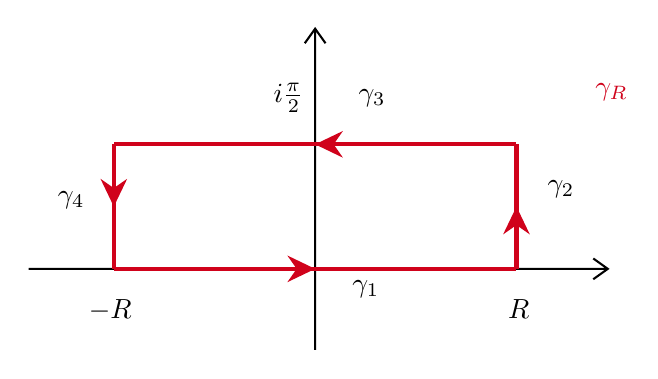
\begin{tikzpicture}[x=0.75pt,y=0.75pt,yscale=-1,xscale=1]
%uncomment if require: \path (0,178); %set diagram left start at 0, and has height of 178

%Shape: Axis 2D [id:dp3537451156705087] 
\draw  (162.5,130.33) -- (441.5,130.33)(300.5,14.63) -- (300.5,169.33) (434.5,125.33) -- (441.5,130.33) -- (434.5,135.33) (295.5,21.63) -- (300.5,14.63) -- (305.5,21.63)  ;
%Straight Lines [id:da6355301965678406] 
\draw [color={rgb, 255:red, 208; green, 2; blue, 27 }  ,draw opacity=1 ][line width=1.5]    (203.5,130.33) -- (397.5,130.33) ;
\draw [shift={(300.5,130.33)}, rotate = 180] [fill={rgb, 255:red, 208; green, 2; blue, 27 }  ,fill opacity=1 ][line width=0.08]  [draw opacity=0] (13.4,-6.43) -- (0,0) -- (13.4,6.44) -- (8.9,0) -- cycle    ;
%Straight Lines [id:da04659866719258687] 
\draw [color={rgb, 255:red, 208; green, 2; blue, 27 }  ,draw opacity=1 ][line width=1.5]    (397.5,70.33) -- (203.5,70.33) ;
\draw [shift={(300.5,70.33)}, rotate = 360] [fill={rgb, 255:red, 208; green, 2; blue, 27 }  ,fill opacity=1 ][line width=0.08]  [draw opacity=0] (13.4,-6.43) -- (0,0) -- (13.4,6.44) -- (8.9,0) -- cycle    ;
%Straight Lines [id:da2855621428556525] 
\draw [color={rgb, 255:red, 208; green, 2; blue, 27 }  ,draw opacity=1 ][line width=1.5]    (397.5,130.33) -- (397.5,70.33) ;
\draw [shift={(397.5,100.33)}, rotate = 450] [fill={rgb, 255:red, 208; green, 2; blue, 27 }  ,fill opacity=1 ][line width=0.08]  [draw opacity=0] (13.4,-6.43) -- (0,0) -- (13.4,6.44) -- (8.9,0) -- cycle    ;
%Straight Lines [id:da09072689237424836] 
\draw [color={rgb, 255:red, 208; green, 2; blue, 27 }  ,draw opacity=1 ][line width=1.5]    (203.5,70.33) -- (203.5,130.33) ;
\draw [shift={(203.5,100.33)}, rotate = 270] [fill={rgb, 255:red, 208; green, 2; blue, 27 }  ,fill opacity=1 ][line width=0.08]  [draw opacity=0] (13.4,-6.43) -- (0,0) -- (13.4,6.44) -- (8.9,0) -- cycle    ;

% Text Node
\draw (392,143.4) node [anchor=north west][inner sep=0.75pt]    {$R$};
% Text Node
\draw (190,143.4) node [anchor=north west][inner sep=0.75pt]    {$-R$};
% Text Node
\draw (279,39.4) node [anchor=north west][inner sep=0.75pt]    {$i\frac{\pi }{2}$};
% Text Node
\draw (434,39.4) node [anchor=north west][inner sep=0.75pt]  [color={rgb, 255:red, 208; green, 2; blue, 27 }  ,opacity=1 ]  {$\gamma _{R}$};
% Text Node
\draw (317,134.4) node [anchor=north west][inner sep=0.75pt]    {$\gamma _{1}$};
% Text Node
\draw (411,86.4) node [anchor=north west][inner sep=0.75pt]    {$\gamma _{2}$};
% Text Node
\draw (320,42.4) node [anchor=north west][inner sep=0.75pt]    {$\gamma _{3}$};
% Text Node
\draw (175,91.4) node [anchor=north west][inner sep=0.75pt]    {$\gamma _{4}$};


\end{tikzpicture}
\end{figure}
\FloatBarrier

La funzione non ha singolarità
\begin{equation*}
\int _{\gamma _{R}} e^{-z^{2}} \ dz=0
\end{equation*}
che è uguale alla somma degli integrali
\begin{equation*}
\int _{\gamma _{R}} e^{-z^{2}} \ dz=\int _{\gamma _{1}} +\int _{\gamma _{2}} +\int _{\gamma _{3}} +\int _{\gamma _{4}}\xrightarrow{R\rightarrow +\infty }\int _{\mathbb{R}} e^{-x^{2}} dx-\int _{\mathbb{R}} e^{-\left( x+\frac{i\xi }{2}\right)^{2}} dx
\end{equation*}
quindi questi due integrali sono uguali al limite
\begin{equation*}
\int _{\mathbb{R}} e^{-\left( x+\frac{i\xi }{2}\right)^{2}} dx=\int _{\mathbb{R}} e^{-x^{2}} dx=\sqrt{\pi }
\end{equation*}
Quindi
\begin{equation*}
\boxed{\mathcal{F}\left\{e^{-x^{2}}\right\} =\sqrt{\pi } e^{-\frac{\xi ^{2}}{4}}}
\end{equation*}
Deduciamo anche, per $\alpha  >0$
\begin{equation*}
\boxed{\mathcal{F}\left\{e^{-\alpha x^{2}}\right\} =\mathcal{F}\left\{e^{-(\sqrt{\alpha } x)^{2}}\right\} =\sqrt{\frac{\pi }{\alpha }} e^{-\frac{\xi ^{2}}{4\alpha }}}
\end{equation*}
\textbf{Equazione differenziale.}

Costruiamo ad hoc un'equazione differenziale
\begin{equation*}
u(x)=e^{-x^{2}} \ \ \Rightarrow \ \ u^{'} (x)=-2xe^{-x^{2}} \ \ \Rightarrow \ \ u^{'} +2xu=0
\end{equation*}
Ora
\begin{equation*}
\mathcal{F}\{u\} =\hat{u} \ \ \ \ \mathcal{F}\{xu\} =i\frac{d}{d\xi }\hat{u} \ \ \ \ \mathcal{F}\{u'\} =i\xi \hat{u} '
\end{equation*}
L'equazione differenziale si riscrive
\begin{equation*}
i\xi \hat{u} +2i\hat{u} '=0\ \ \Rightarrow \ \ \hat{u} '+\frac{\xi }{2}\hat{u} =0\ \ \Rightarrow \ \ \hat{u}( \xi ) =Ce^{-\int \frac{\xi }{2} d\xi } =Ce^{-\xi ^{2} /4}
\end{equation*}
Determiniamo la costante
\begin{equation*}
C=\hat{u}( 0) =\int _{\mathbb{R}} e^{-i0x} u( x) dx=\int _{\mathbb{R}} u( x) dx=\int _{\mathbb{R}} e^{-x^{2}} dx=\sqrt{\pi }
\end{equation*}
Allora
\begin{equation*}
\boxed{\hat{u}( \xi ) =\sqrt{\pi } e^{-\xi ^{2} /4}}
\end{equation*}
\Soluzione

\fg{0.7}{15-4}
\begin{equation*}
\mathcal{F}\left\{\frac{1}{\cosh x}\right\} =\int _{\mathbb{R}}\frac{e^{-i\xi x}}{\cosh x} dx=\int _{\mathbb{R}}\frac{2e^{-i\xi x}}{e^{x} +e^{-x}} dx\ \ \Rightarrow \ \ f( x) =\frac{2e^{-i\xi z}}{e^{z} +e^{-z}}
\end{equation*}
Tutte le singolarità sono tutti i punti del piano complesso in cui si annulla il denominatore 
\begin{equation*}
e^{z} +e^{-z} =e^{-z} (e^{2z} +1)=0\ \ \Leftrightarrow \ \ 2z=i\pi +2k\pi \ \ \Leftrightarrow \ \ z=i\frac{\pi }{2} +k\pi ,\ \ k\in \mathbb{Z}
\end{equation*}
Disegno il grafico con il solito rettangolo della gamma che contenga solo un residuo.


\begin{figure}[htpb]
	\centering
\tikzset{every picture/.style={line width=0.75pt}} %set default line width to 0.75pt        

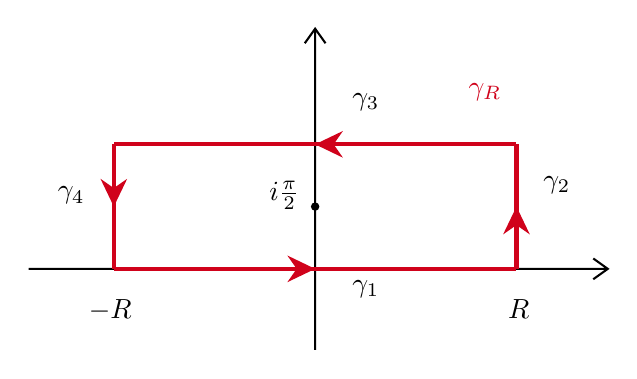
\begin{tikzpicture}[x=0.75pt,y=0.75pt,yscale=-1,xscale=1]
%uncomment if require: \path (0,178); %set diagram left start at 0, and has height of 178

%Shape: Axis 2D [id:dp7510536935747429] 
\draw  (162.5,130.33) -- (441.5,130.33)(300.5,14.63) -- (300.5,169.33) (434.5,125.33) -- (441.5,130.33) -- (434.5,135.33) (295.5,21.63) -- (300.5,14.63) -- (305.5,21.63)  ;
%Straight Lines [id:da06806358271411694] 
\draw [color={rgb, 255:red, 208; green, 2; blue, 27 }  ,draw opacity=1 ][line width=1.5]    (203.5,130.33) -- (397.5,130.33) ;
\draw [shift={(300.5,130.33)}, rotate = 180] [fill={rgb, 255:red, 208; green, 2; blue, 27 }  ,fill opacity=1 ][line width=0.08]  [draw opacity=0] (13.4,-6.43) -- (0,0) -- (13.4,6.44) -- (8.9,0) -- cycle    ;
%Straight Lines [id:da47939213158777694] 
\draw [color={rgb, 255:red, 208; green, 2; blue, 27 }  ,draw opacity=1 ][line width=1.5]    (397.5,70.33) -- (203.5,70.33) ;
\draw [shift={(300.5,70.33)}, rotate = 360] [fill={rgb, 255:red, 208; green, 2; blue, 27 }  ,fill opacity=1 ][line width=0.08]  [draw opacity=0] (13.4,-6.43) -- (0,0) -- (13.4,6.44) -- (8.9,0) -- cycle    ;
%Straight Lines [id:da9055165704816575] 
\draw [color={rgb, 255:red, 208; green, 2; blue, 27 }  ,draw opacity=1 ][line width=1.5]    (397.5,130.33) -- (397.5,70.33) ;
\draw [shift={(397.5,100.33)}, rotate = 450] [fill={rgb, 255:red, 208; green, 2; blue, 27 }  ,fill opacity=1 ][line width=0.08]  [draw opacity=0] (13.4,-6.43) -- (0,0) -- (13.4,6.44) -- (8.9,0) -- cycle    ;
%Straight Lines [id:da5009557145102899] 
\draw [color={rgb, 255:red, 208; green, 2; blue, 27 }  ,draw opacity=1 ][line width=1.5]    (203.5,70.33) -- (203.5,130.33) ;
\draw [shift={(203.5,100.33)}, rotate = 270] [fill={rgb, 255:red, 208; green, 2; blue, 27 }  ,fill opacity=1 ][line width=0.08]  [draw opacity=0] (13.4,-6.43) -- (0,0) -- (13.4,6.44) -- (8.9,0) -- cycle    ;
%Shape: Circle [id:dp4183664382061272] 
\draw  [fill={rgb, 255:red, 0; green, 0; blue, 0 }  ,fill opacity=1 ] (299,100.33) .. controls (299,99.5) and (299.67,98.83) .. (300.5,98.83) .. controls (301.33,98.83) and (302,99.5) .. (302,100.33) .. controls (302,101.16) and (301.33,101.83) .. (300.5,101.83) .. controls (299.67,101.83) and (299,101.16) .. (299,100.33) -- cycle ;

% Text Node
\draw (392,143.4) node [anchor=north west][inner sep=0.75pt]    {$R$};
% Text Node
\draw (190,143.4) node [anchor=north west][inner sep=0.75pt]    {$-R$};
% Text Node
\draw (277,86.4) node [anchor=north west][inner sep=0.75pt]    {$i\frac{\pi }{2}$};
% Text Node
\draw (373,39.4) node [anchor=north west][inner sep=0.75pt]  [color={rgb, 255:red, 208; green, 2; blue, 27 }  ,opacity=1 ]  {$\gamma _{R}$};
% Text Node
\draw (317,134.4) node [anchor=north west][inner sep=0.75pt]    {$\gamma _{1}$};
% Text Node
\draw (409,84.4) node [anchor=north west][inner sep=0.75pt]    {$\gamma _{2}$};
% Text Node
\draw (317,44.4) node [anchor=north west][inner sep=0.75pt]    {$\gamma _{3}$};
% Text Node
\draw (175,89.4) node [anchor=north west][inner sep=0.75pt]    {$\gamma _{4}$};


\end{tikzpicture}
\end{figure}
\FloatBarrier

Calcolo
\begin{equation*}
\begin{aligned}
\int _{\gamma _{R}} f(z)dz & =2\pi i\cdotp \mathrm{Res}\left( f,z=\frac{i\pi }{2}\right) =2\pi i\left. \frac{2e^{-i\xi z}}{e^{z} -e^{-z}}\right| _{z=i\pi /2}\\
 & =2\pi i\cdotp \frac{2e^{\xi \frac{\pi }{2}}}{e^{\frac{i\pi }{2}} -e^{-\frac{i\pi }{2}}} =2\pi i\cdotp \frac{2e^{\xi \frac{\pi }{2}}}{i-( -i)} =2\pi e^{\xi \frac{\pi }{2}}
\end{aligned}
\end{equation*}
Scriviamo i vari pezzi
\begin{align*}
\int _{\gamma _{R}} f( z) dz & =2\pi e^{\frac{\xi \pi }{2}} =\int _{\gamma _{1}} +\int _{\gamma _{2}} +\int _{\gamma _{3}} +\int _{\gamma _{4}}\\
 & \\
\int _{\gamma _{1}} & =\int ^{R}_{-R}\frac{e^{-i\xi x}}{\cosh (x)} dx\xrightarrow{R\rightarrow +\infty }\mathcal{F}\left\{\frac{1}{\cosh (x)}\right\}\\
 & \\
\int _{\gamma _{2}} & =2\int ^{\pi i}_{0}\frac{e^{-i\xi (R+iy)}}{e^{R+iy} +e^{-R-iy}} idy\\
\left| \int _{\gamma _{2}}\right|  & =2\left| \int ^{\pi }_{0}\frac{e^{-i\xi R} e^{y}}{e^{R}\left( e^{iy} +e^{-2R-iy}\right)} idy\right| \leqslant \frac{2}{e^{R}}\underbrace{\int ^{\pi }_{0}\left| \frac{e^{y}}{e^{iy} +e^{-2R-iy}}\right| dy}_{\text{limitata}}\xrightarrow{R\rightarrow +\infty } 0\\
 & \\
\int _{\gamma _{3}} = & -\int ^{R}_{-R}\frac{2e^{-i\xi ( x+i\pi )}}{e^{x+i\pi } +e^{-x-i\pi }} dx=\int ^{R}_{-R}\frac{2e^{-i\xi x} e^{\pi \xi }}{e^{x} +e^{-x}} dx\\
 & =e^{\pi \xi }\int ^{R}_{-R}\frac{e^{-i\xi x}}{\frac{e^{x} +e^{-x}}{2}} dx\xrightarrow{R\rightarrow +\infty } e^{\pi \xi }\mathcal{F}\left\{\frac{1}{\cosh (x)}\right\}\\
 & \\
\left| \int _{\gamma _{4}}\right|  & \xrightarrow{R\rightarrow +\infty } 0
\end{align*}
In totale avremo
\begin{equation*}
2\pi e^{\xi \frac{\pi }{2}} =\int _{\gamma _{R}} f( z) dz\xrightarrow{R\rightarrow +\infty }\mathcal{F}\left\{\frac{1}{\cosh (x)}\right\}\left( 1+e^{\pi \xi }\right)
\end{equation*}
Dunque
\begin{equation*}
\mathcal{F}\left\{\frac{1}{\cosh (x)}\right\} =\frac{2\pi e^{\xi \frac{\pi }{2}}}{e^{\pi \xi } +1} =\frac{2\pi }{e^{\xi \frac{\pi }{2}} +e^{-\xi \frac{\pi }{2}}} =\frac{\pi }{\cosh\left(\frac{\pi }{2} \xi \right)}
\end{equation*}
\Soluzione

\fg{0.7}{15-5}
\begin{equation*}
\mathcal{F}\left\{\frac{1}{\left( 1+x^{2}\right)^{2}}\right\} =\int _{\mathbb{R}}\frac{e^{-i\xi x}}{\left( 1+x^{2}\right)^{2}} dx
\end{equation*}
$f$ pari, allora $\hat{f}$ pari.

Poniamo\footnote{Con $f$ si indica sia la funzione data che quella integranda, ma sono due funzioni che differiscono per il numeratore. Non facciamo troppo i pignoli.}
\begin{equation*}
f( z) =\frac{e^{-i\xi z}}{\left( 1+z^{2}\right)^{2}}
\end{equation*}
$z=\pm i$ sono poli del II ordine.

Giochiamo con i residui utilizzando il Lemma di Jordan
\begin{equation*}
\int _{\gamma _{R}} g( z) e^{i\alpha z} dz
\end{equation*}
\textit{Quale circonferenza bisogna prendere?}

Se $\alpha $ è positivo il lemma di Jordan parla della semicirconferenza superiore mentre se $\alpha $ è negativo della semicirconferenza inferiore.

Nel nostro caso si parla di $-\xi $ per calcolare quanto vale questa trasformata avremo che se $\xi $ è negativo avremo bisogno del semipiano superiore, se $\xi $ è positivo di quello inferiore. Essendo simmetrici si sfrutta il risultato teorico della parità.


\begin{figure}[htpb]
	\centering
\tikzset{every picture/.style={line width=0.75pt}} %set default line width to 0.75pt        

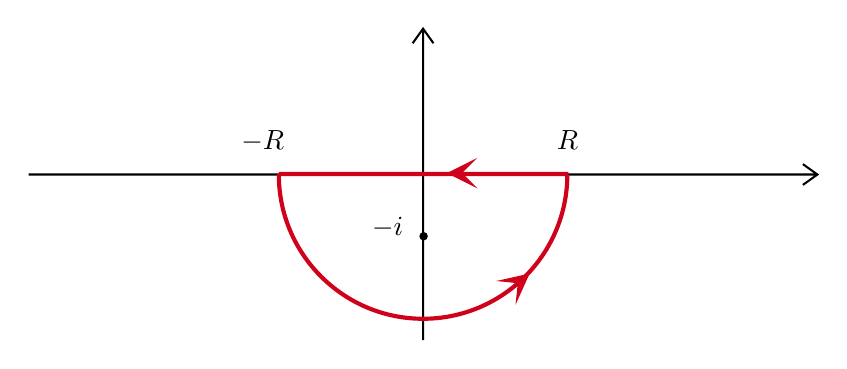
\begin{tikzpicture}[x=0.75pt,y=0.75pt,yscale=-1,xscale=1]
%uncomment if require: \path (0,172); %set diagram left start at 0, and has height of 172

%Shape: Axis 2D [id:dp752436124621402] 
\draw  (110,80.25) -- (490,80.25)(300,10) -- (300,160) (483,75.25) -- (490,80.25) -- (483,85.25) (295,17) -- (300,10) -- (305,17)  ;
%Shape: Arc [id:dp579891374669032] 
\draw  [draw opacity=0][line width=1.5]  (369.5,80.77) .. controls (369.22,118.92) and (338.21,149.75) .. (300,149.75) .. controls (261.62,149.75) and (230.5,118.63) .. (230.5,80.25) .. controls (230.5,80.16) and (230.5,80.07) .. (230.5,79.98) -- (300,80.25) -- cycle ; \draw  [color={rgb, 255:red, 208; green, 2; blue, 27 }  ,draw opacity=1 ][line width=1.5]  (369.5,80.77) .. controls (369.22,118.92) and (338.21,149.75) .. (300,149.75) .. controls (261.62,149.75) and (230.5,118.63) .. (230.5,80.25) .. controls (230.5,80.16) and (230.5,80.07) .. (230.5,79.98) ;
%Shape: Circle [id:dp9196698365325671] 
\draw  [fill={rgb, 255:red, 0; green, 0; blue, 0 }  ,fill opacity=1 ] (298.75,109.99) .. controls (298.75,109.16) and (299.42,108.49) .. (300.25,108.49) .. controls (301.08,108.49) and (301.75,109.16) .. (301.75,109.99) .. controls (301.75,110.82) and (301.08,111.49) .. (300.25,111.49) .. controls (299.42,111.49) and (298.75,110.82) .. (298.75,109.99) -- cycle ;
\draw  [draw opacity=0][fill={rgb, 255:red, 208; green, 2; blue, 27 }  ,fill opacity=1 ] (326.2,86.94) -- (311.45,79.56) -- (326.2,72.19) -- (318.83,79.56) -- cycle ;
\draw  [draw opacity=0][fill={rgb, 255:red, 208; green, 2; blue, 27 }  ,fill opacity=1 ] (335.24,131.55) -- (351.34,127.96) -- (344.55,143) -- (345.62,132.62) -- cycle ;
%Straight Lines [id:da3950283299762536] 
\draw [color={rgb, 255:red, 208; green, 2; blue, 27 }  ,draw opacity=1 ][line width=1.5]    (230.5,79.98) -- (370,80) ;

% Text Node
\draw (211,57.4) node [anchor=north west][inner sep=0.75pt]    {$-R$};
% Text Node
\draw (363,57.4) node [anchor=north west][inner sep=0.75pt]    {$R$};
% Text Node
\draw (274,99.4) node [anchor=north west][inner sep=0.75pt]  [font=\normalsize]  {$-i$};


\end{tikzpicture}
\end{figure}
\FloatBarrier

Per $\xi  >0$
\begin{equation*}
\int _{R}\frac{e^{-i\xi x}}{\left( 1+x^{2}\right)^{2}} dx=-2\pi i\cdotp \mathrm{Res}( f,z=-i)
\end{equation*}
Il segno meno è giustificato dal fatto che percorriamo la semicirconferenza in senso \textit{antiorario}.

Il residuo allora sarà pari a
\begin{equation*}
\begin{aligned}
\mathrm{Res}( f,z=-i) & =\left. \frac{d}{dz}\frac{e^{-i\xi z}}{( z-i)^{2}}\right| _{z=-i}\\
 & =\left. \frac{-i\xi e^{-i\xi z}( z-i)^{2} -e^{-i\xi z} 2(z-i)}{( z-i)^{4}}\right| _{z=-i}\\
 & =\frac{e^{-\xi }( 4i+4i\xi )}{16} =i\frac{e^{-\xi }}{4} (1+\xi )
\end{aligned}
\end{equation*}
La trasformata vale quindi
\begin{equation*}
\mathcal{F}\left\{\frac{1}{\left( 1+x^{2}\right)^{2}}\right\} =-2\pi i\cdotp i\frac{e^{-\xi }}{4} (1+\xi )=\frac{\pi }{2} e^{-\xi }( 1+\xi ) \ \ \ \ \xi  >0
\end{equation*}
Per le $\xi < 0$ basta raddoppiare
\begin{equation*}
\hat{f}( \xi ) =\frac{\pi }{2} e^{-| \xi | } (1+| \xi | )
\end{equation*}
\Soluzione

Vediamo il grafico di $u(x)=1/\sqrt{|x|}$

\fg{0.7}{15-6}

Notiamo che $u\notin L^{1}$ perché all'infinito va a zero troppo lentamente e neanche $u\notin L^{2}$, in tal caso sarebbe asintotica a $1/x$ per $x\rightarrow \infty $, che non è integrabile.

Possiamo considerare $u$ come una distribuzione temperata, cioè $u\in \mathcal{S}^{'}(\mathbb{R})$.

Possiamo prendere una successione di funzioni $u_{n}$ che l'approssimano nel senso delle distribuzioni temperate
\begin{equation*}
u_{n}( x) =u( x) \chi _{( -n,n)}( x) \ \ \ \ u_{n} \in L^{1} (\mathbb{R} )
\end{equation*}
Considerando la dualità con una qualsiasi funzione dello spazio di Schwartz questa sarà pari a:
\begin{gather*}
\langle ( u-u_{n}) ,\psi \rangle =\int ^{-n}_{-\infty }\frac{1}{\sqrt{| x| }} \psi ( x) dx+\ \int ^{+\infty }_{n}\frac{1}{\sqrt{x}} \psi ( x) dx\\
\\
| \langle ( u-u_{n}) ,\ \psi \rangle | \leqslant \frac{1}{\sqrt{n}} \ \int _{\mathbb{R}}| \psi ( x)| dx\xrightarrow{n\rightarrow \infty } 0\ \ \Rightarrow \ \ u_{n}\xrightarrow[\mathcal{S} ']{n\rightarrow \infty } u
\end{gather*}
Ne consegue che possiamo scrivere:
\begin{equation*}
\mathcal{F}\{u\} =\lim _{n\rightarrow \infty }\mathcal{F}\{u_{n}\}
\end{equation*}
Calcoliamo le trasformate delle $u_{n}$ in senso classico
\begin{equation*}
\mathcal{F}\{u_{n}\} =\int _{\mathbb{R}}\frac{e^{-i\xi x}}{\sqrt{|} x|} \chi _{[-n,n]} (u)dx=\int ^{n}_{-n}\frac{\cos( \xi x) -i\sin (\xi x)}{\sqrt{| x| }} dx=2\int ^{n}_{0}\frac{\cos( \xi x)}{\sqrt{x}} dx
\end{equation*}
Sostituzione
\begin{equation*}
\xi x=t^{2} \ \ \Rightarrow \ \ dx=\frac{2}{\xi } tdt
\end{equation*}
Allora
\begin{equation*}
=2\int ^{\sqrt{\xi n}}_{0}\frac{\cos\left( t^{2}\right)}{\sqrt{\frac{t^{2}}{\xi }}}\frac{2t}{\xi } dt=\frac{4}{\sqrt{\xi }} \ \int ^{\sqrt{\xi n}}_{0}\cos\left( t^{2}\right) dt=
\end{equation*}
Ricordiamo l'integrale di Fresnel
\begin{equation*}
\int ^{+\infty }_{0}\cos\left( x^{2}\right) dx=\sqrt{\frac{\pi }{8}}
\end{equation*}
Quindi, la trasformata sarà pari a
\begin{equation*}
\mathcal{F}\{u\} =\lim _{n\rightarrow \infty }\mathcal{F}\{u_{n}\} =\lim _{n\rightarrow \infty }\frac{4}{\sqrt{| \xi | }} \ \int ^{\sqrt{| \xi | n}}_{0}\cos\left( t^{2}\right) dt=\frac{4}{\sqrt{| \xi | }} \ \sqrt{\frac{\pi }{8}} =\ \sqrt{\frac{2\pi }{| \xi | }}
\end{equation*}
\chapter{Esercitazione 8 - Potrich}
\ParteEsercizi
\begin{definition}
Sia $u\in L^{1}(\mathbb{R})$. Si dice \textbf{Trasformata di Fourier} di $u$ la funzione $\hat{u} :\mathbb{R}\rightarrow \mathbb{C}$ definita da
\begin{equation*}
\hat{u}( \xi ) =\int _{\mathbb{R}} e^{-i\xi x} u( x) dx
\end{equation*}
\end{definition}
\begin{theorem}
[Proprietà] Ecco alcune utili proprietà della trasformata di Fourier.
\begin{itemize}
\item Scaling\begin{equation*}
u( ax) \ \ \rightarrow \ \ \frac{1}{| a| }\hat{u}\left(\frac{\xi }{a}\right)
\end{equation*}
\item Shifting\begin{equation*}
u( x-a) \ \ \rightarrow \ \ e^{-ia\xi }\hat{u}( \xi )
\end{equation*}
\item Modulazione\begin{gather*}
u( x) e^{iax} \ \ \rightarrow \ \ \hat{u}( \xi -a)\\
u( x)\cos( \xi _{0} x) \ \ \rightarrow \ \ \frac{1}{2}[\hat{u}( \xi -\xi _{0}) +\hat{u}( \xi +\xi _{0})]
\end{gather*}
\item Linearità\begin{equation*}
\mathcal{F}\{\alpha u+\beta v\} =\alpha \mathcal{F}\{u\} +\beta \mathcal{F}\{v\} \ \ \forall \alpha ,\beta \in \mathbb{R} ,\ \forall u,v\in L^{1}(\mathbb{R})
\end{equation*}
\item Derivazione\begin{equation*}
\widehat{u'}( \xi ) =i\xi \hat{u}( \xi )
\end{equation*}
\end{itemize}
\end{theorem}
\Esercizio{Una trasformata notevole}

Calcolare la trasformata di Fourier di
\begin{equation*}
u( x) =\frac{1}{1+x^{2}} ,\ \ x\in \mathbb{R}
\end{equation*}
\Esercizio{Trasformata della Gaussiana}

Calcolare la trasformata di Fourier della funzione Gaussiana
\begin{equation*}
u( x) =e^{-x^{2}} ,\ x\in \mathbb{R}
\end{equation*}
\Esercizio{}

Calcolare la trasformata di Fourier di
\begin{equation*}
f( x) =\frac{\sin x}{\left( 1+x^{2}\right)\left( 4+x^{2}\right)}
\end{equation*}
\Esercizio{}

Calcolare la trasformata di Fourier di\begin{equation*}
u( x) =\frac{2\cos x}{1+x^{2}}
\end{equation*}
\Esercizio{}

Determinare l'espressione analitica di
\begin{equation*}
f( \tau ) =\int _{\mathbb{R}} e^{-i\left( \tau ^{2} -2\right) x}\frac{\cos( 2x)}{1+x^{2}} dx
\end{equation*}
\Esercizio{}

Sia
\begin{equation*}
f( x) =\begin{cases}
1, & 0< x< 1\\
-1, & -1< x< 0
\end{cases}
\end{equation*}
\begin{enumerate}
\item Calcolare la trasformata di Fourier di $f( x)$
\item Calcolare la trasformata di Fourier di $g( x) =xf( x)$
\end{enumerate}
\Esercizio{}

Sia $H$ la funzione di Heaviside
\begin{equation*}
H( t) =\begin{cases}
1, & t\geqslant 0\\
0, & t< 0
\end{cases}
\end{equation*}
\begin{enumerate}
\item Calcolare la trasformata di Fourier di\begin{equation*}
f( x) =\left( 1-x^{2}\right) H\left( 1-x^{2}\right)
\end{equation*}
\item Utilizzare il risultato trovato per calcolare\begin{equation*}
\int ^{+\infty }_{0}\frac{x\cos x-\sin x}{x^{3}}\cos\left(\frac{x}{2}\right) dx
\end{equation*}
\end{enumerate}
\ParteSoluzioni
\Soluzione

Per definizione
\begin{equation*}
\hat{u}( \xi ) =\int _{\mathbb{R}} e^{-i\xi x} u( x) dx
\end{equation*}
Consideriamo la funzione analitica
\begin{equation*}
f( z) =\frac{1}{1+z^{2}}
\end{equation*}
le cui singolarità si trovano in
\begin{equation*}
1+z^{2} =0\ \ \Leftrightarrow \ \ z=\pm i
\end{equation*}
e sono dei poli semplici.


\begin{figure}[htpb]
	\centering
\tikzset{every picture/.style={line width=0.75pt}} %set default line width to 0.75pt        

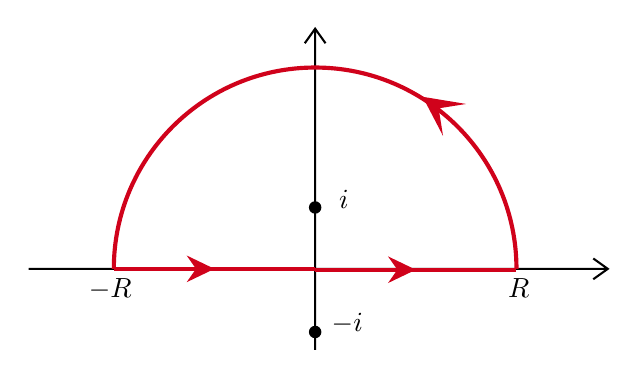
\begin{tikzpicture}[x=0.75pt,y=0.75pt,yscale=-1,xscale=1]
%uncomment if require: \path (0,181); %set diagram left start at 0, and has height of 181

%Shape: Axis 2D [id:dp6994241881147589] 
\draw  (162.5,130.33) -- (441.5,130.33)(300.5,14.63) -- (300.5,169.33) (434.5,125.33) -- (441.5,130.33) -- (434.5,135.33) (295.5,21.63) -- (300.5,14.63) -- (305.5,21.63)  ;
%Straight Lines [id:da47956119812522835] 
\draw [color={rgb, 255:red, 208; green, 2; blue, 27 }  ,draw opacity=1 ][line width=1.5]    (300.5,130.75) -- (397.5,130.75) ;
\draw [shift={(349,130.75)}, rotate = 180] [fill={rgb, 255:red, 208; green, 2; blue, 27 }  ,fill opacity=1 ][line width=0.08]  [draw opacity=0] (13.4,-6.43) -- (0,0) -- (13.4,6.44) -- (8.9,0) -- cycle    ;
%Shape: Arc [id:dp5355059210550983] 
\draw  [draw opacity=0][line width=1.5]  (203.5,130.33) .. controls (203.5,76.76) and (246.93,33.33) .. (300.5,33.33) .. controls (354.07,33.33) and (397.5,76.76) .. (397.5,130.33) -- (300.5,130.33) -- cycle ; \draw  [color={rgb, 255:red, 208; green, 2; blue, 27 }  ,draw opacity=1 ][line width=1.5]  (203.5,130.33) .. controls (203.5,76.76) and (246.93,33.33) .. (300.5,33.33) .. controls (354.07,33.33) and (397.5,76.76) .. (397.5,130.33) ;
%Straight Lines [id:da2269425139728658] 
\draw [color={rgb, 255:red, 208; green, 2; blue, 27 }  ,draw opacity=1 ][line width=1.5]    (203.5,130.33) -- (300.5,130.33) ;
\draw [shift={(252,130.33)}, rotate = 180] [fill={rgb, 255:red, 208; green, 2; blue, 27 }  ,fill opacity=1 ][line width=0.08]  [draw opacity=0] (13.4,-6.43) -- (0,0) -- (13.4,6.44) -- (8.9,0) -- cycle    ;
\draw  [draw opacity=0][fill={rgb, 255:red, 208; green, 2; blue, 27 }  ,fill opacity=1 ] (362.12,66.27) -- (352.31,47.43) -- (373.27,50.88) -- (360,53) -- cycle ;
%Shape: Circle [id:dp54653528391848] 
\draw  [draw opacity=0][fill={rgb, 255:red, 0; green, 0; blue, 0 }  ,fill opacity=1 ] (297.5,100.75) .. controls (297.5,99.1) and (298.84,97.75) .. (300.5,97.75) .. controls (302.16,97.75) and (303.5,99.1) .. (303.5,100.75) .. controls (303.5,102.41) and (302.16,103.75) .. (300.5,103.75) .. controls (298.84,103.75) and (297.5,102.41) .. (297.5,100.75) -- cycle ;
%Shape: Circle [id:dp23929766105583639] 
\draw  [draw opacity=0][fill={rgb, 255:red, 0; green, 0; blue, 0 }  ,fill opacity=1 ] (297.5,160.75) .. controls (297.5,159.1) and (298.84,157.75) .. (300.5,157.75) .. controls (302.16,157.75) and (303.5,159.1) .. (303.5,160.75) .. controls (303.5,162.41) and (302.16,163.75) .. (300.5,163.75) .. controls (298.84,163.75) and (297.5,162.41) .. (297.5,160.75) -- cycle ;

% Text Node
\draw (392,133.4) node [anchor=north west][inner sep=0.75pt]    {$R$};
% Text Node
\draw (190,133.4) node [anchor=north west][inner sep=0.75pt]    {$-R$};
% Text Node
\draw (310.5,90.9) node [anchor=north west][inner sep=0.75pt]    {$i$};
% Text Node
\draw (307,150.4) node [anchor=north west][inner sep=0.75pt]    {$-i$};


\end{tikzpicture}
\end{figure}
\FloatBarrier

Osserviamo che $| f( z)| \sim \frac{1}{z^{2}}$ per $| z| \rightarrow +\infty $, allora col teorema dei residui e il lemma di Jordan
\begin{equation*}
\int ^{+\infty }_{-\infty } e^{-i\xi x}\frac{1}{1+x^{2}} dx=2\pi i\cdotp \mathrm{Res}\left(\frac{e^{-i\xi z}}{1+z^{2}} ,z=i\right) =\pi e^{\xi } \ \ \forall \xi < 0
\end{equation*}
\begin{nb}
Se $f$ è pari, allora $\hat{f}$ è pari.
\end{nb}
I valori per $\xi  >0$ si ottengono da quelli negativi imponendo che $\hat{f}$ sia pari
\begin{nb}
$f\in L^{1} \Rightarrow \hat{f}$ è continua.
\end{nb}
Il valore in $0$ si ottiene per continuità.
\begin{equation*}
\Rightarrow \ \ \boxed{\hat{f}( \xi ) =\pi e^{-| \xi | } \ \ \forall \xi \in \mathbb{R}}
\end{equation*}
\Soluzione
\begin{equation*}
\hat{u}( \xi ) =\int _{\mathbb{R}} e^{-i\xi x} u( x) dx=\int _{\mathbb{R}} e^{-i\xi x} e^{-x^{2}} dx
\end{equation*}
\textbf{\underline{Metodo con l'analisi complessa}}
\begin{equation*}
\hat{u}( \xi ) =\int _{\mathbb{R}} e^{-i\xi x} e^{-x^{2}} dx=\int _{\mathbb{R}} e^{-\left( i\xi x+x^{2}\right)} dx
\end{equation*}
Completiamo il quadrato
\begin{equation*}
\int _{\mathbb{R}} e^{-\left( i\xi x+x^{2}\right)} dx=e^{-\frac{\xi ^{2}}{4}}\int _{\mathbb{R}} e^{-\left( x+\frac{i\xi }{2}\right)^{2}} dx
\end{equation*}
Sfruttiamo la seguente uguaglianza
\begin{equation*}
\int ^{+\infty }_{-\infty } e^{-( x+ib)^{2}} dx\overset{( *)}{=}\int ^{+\infty }_{-\infty } e^{-x^{2}} dx=\sqrt{\pi } \ \ \Rightarrow \ \ \boxed{\hat{u}( \xi ) =\sqrt{\pi } e^{-\frac{\xi ^{2}}{4}}}
\end{equation*}
Resta da provare $( *)$. Consideriamo la funzione analitica intera (senza singolarità) $z\mapsto e^{-z^{2}}$, prolungamento analitico di $e^{-x^{2}} ,x\in \mathbb{R}$.


\begin{figure}[htpb]
	\centering
\tikzset{every picture/.style={line width=0.75pt}} %set default line width to 0.75pt        

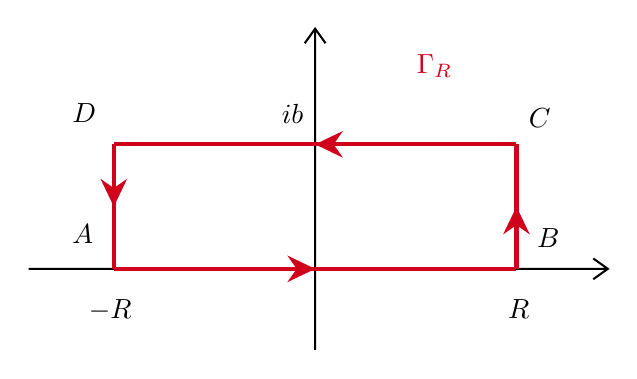
\begin{tikzpicture}[x=0.75pt,y=0.75pt,yscale=-1,xscale=1]
%uncomment if require: \path (0,178); %set diagram left start at 0, and has height of 178

%Shape: Axis 2D [id:dp08896652720756437] 
\draw  (162.5,130.33) -- (441.5,130.33)(300.5,14.63) -- (300.5,169.33) (434.5,125.33) -- (441.5,130.33) -- (434.5,135.33) (295.5,21.63) -- (300.5,14.63) -- (305.5,21.63)  ;
%Straight Lines [id:da3929751532760877] 
\draw [color={rgb, 255:red, 208; green, 2; blue, 27 }  ,draw opacity=1 ][line width=1.5]    (203.5,130.33) -- (397.5,130.33) ;
\draw [shift={(300.5,130.33)}, rotate = 180] [fill={rgb, 255:red, 208; green, 2; blue, 27 }  ,fill opacity=1 ][line width=0.08]  [draw opacity=0] (13.4,-6.43) -- (0,0) -- (13.4,6.44) -- (8.9,0) -- cycle    ;
%Straight Lines [id:da9171312565843239] 
\draw [color={rgb, 255:red, 208; green, 2; blue, 27 }  ,draw opacity=1 ][line width=1.5]    (397.5,70.33) -- (203.5,70.33) ;
\draw [shift={(300.5,70.33)}, rotate = 360] [fill={rgb, 255:red, 208; green, 2; blue, 27 }  ,fill opacity=1 ][line width=0.08]  [draw opacity=0] (13.4,-6.43) -- (0,0) -- (13.4,6.44) -- (8.9,0) -- cycle    ;
%Straight Lines [id:da891206314069279] 
\draw [color={rgb, 255:red, 208; green, 2; blue, 27 }  ,draw opacity=1 ][line width=1.5]    (397.5,130.33) -- (397.5,70.33) ;
\draw [shift={(397.5,100.33)}, rotate = 450] [fill={rgb, 255:red, 208; green, 2; blue, 27 }  ,fill opacity=1 ][line width=0.08]  [draw opacity=0] (13.4,-6.43) -- (0,0) -- (13.4,6.44) -- (8.9,0) -- cycle    ;
%Straight Lines [id:da5821046363194966] 
\draw [color={rgb, 255:red, 208; green, 2; blue, 27 }  ,draw opacity=1 ][line width=1.5]    (203.5,70.33) -- (203.5,130.33) ;
\draw [shift={(203.5,100.33)}, rotate = 270] [fill={rgb, 255:red, 208; green, 2; blue, 27 }  ,fill opacity=1 ][line width=0.08]  [draw opacity=0] (13.4,-6.43) -- (0,0) -- (13.4,6.44) -- (8.9,0) -- cycle    ;

% Text Node
\draw (392,143.4) node [anchor=north west][inner sep=0.75pt]    {$R$};
% Text Node
\draw (190,143.4) node [anchor=north west][inner sep=0.75pt]    {$-R$};
% Text Node
\draw (182,107.4) node [anchor=north west][inner sep=0.75pt]    {$A$};
% Text Node
\draw (182,49.4) node [anchor=north west][inner sep=0.75pt]    {$D$};
% Text Node
\draw (402,51.4) node [anchor=north west][inner sep=0.75pt]    {$C$};
% Text Node
\draw (406,109.4) node [anchor=north west][inner sep=0.75pt]    {$B$};
% Text Node
\draw (283,49.4) node [anchor=north west][inner sep=0.75pt]    {$ib$};
% Text Node
\draw (348,25.4) node [anchor=north west][inner sep=0.75pt]  [color={rgb, 255:red, 208; green, 2; blue, 27 }  ,opacity=1 ]  {$\Gamma _{R}$};


\end{tikzpicture}
\end{figure}
\FloatBarrier

con
\begin{equation*}
\begin{aligned}
A & =-R\\
B & =R\\
C & =R+ib\\
D & =-R+ib
\end{aligned} \ \ \ \ \forall R >0,\forall b >0
\end{equation*}
Per il teorema dell'integrale nullo di Cauchy
\begin{equation*}
\oint _{\Gamma _{R}} e^{-z^{2}} dz=0
\end{equation*}
Sul pezzo $BC$ affermiamo
\begin{equation*}
\lim\limits _{R\rightarrow +\infty }\int ^{C}_{B} e^{-z^{2}} dz=0
\end{equation*}
dato che se $R >2b$ si ottiene, per ogni $z\in BC$,
\begin{gather*}
z=| z| (\cos \vartheta +i\sin \vartheta )\\
\left| e^{-z^{2}}\right| =e^{\mathrm{Re}\left( -z^{2}\right)} =e^{-| z| ^{2}\cos 2\vartheta } \leqslant e^{-R^{2}\cos 2\vartheta } =e^{-R^{2}\left(\cos^{2} \vartheta -\sin^{2} \vartheta \right)} \leqslant e^{-\frac{R^{2}}{4}}\xrightarrow{R\rightarrow +\infty } 0
\end{gather*}
Analogamente
\begin{equation*}
\lim\limits _{R\rightarrow +\infty }\int ^{A}_{D} e^{-z^{2}} dz=0
\end{equation*}
Allora possiamo dire
\begin{equation*}
\Rightarrow \ \ \int ^{B}_{A} e^{-z^{2}} dz=-\int ^{D}_{C} e^{-z^{2}} dz+o\left(\frac{1}{R}\right)
\end{equation*}
Passando al limite per $R\rightarrow +\infty $ si ottiene $( *)$.



\underline{\textbf{Metodo alternativo con equazioni differenziali.}}

Consideriamo l'equazione differenziale lineare omogenea del primo ordine
\begin{equation*}
u'( x) =-2xu( x) ,\ \ x\in \mathbb{R}
\end{equation*}
in quanto $e^{-x^{2}}$ è soluzione di questa equazione differenziale. Andiamo a trasformare tutti i termini di questa equazione.
\begin{equation*}
i\xi \hat{u}( \xi ) =-2i\hat{u} '( \xi ) \ \ \Rightarrow \ \ \hat{u}( \xi ) =Ce^{-\frac{\xi ^{2}}{4}}
\end{equation*}
per cui si deve scegliere
\begin{equation*}
C=\hat{u}( 0) =\int _{\mathbb{R}} e^{-i\xi x} e^{-t^{2}} dt\overset{\xi =0}{=}\int _{\mathbb{R}} e^{-t^{2}} dt=\sqrt{\pi }
\end{equation*}
Concludiamo che
\begin{equation*}
\boxed{\hat{u}( \xi ) =\sqrt{\pi } e^{-\frac{\xi ^{2}}{4}}}
\end{equation*}
\Soluzione

Poniamo
\begin{gather*}
u( x) =\frac{1}{\left( 1+x^{2}\right)\left( 4+x^{2}\right)}\\
\Rightarrow \ \ \hat{u}( \xi ) =\int _{\mathbb{R}} e^{-i\xi x} u( x) dx=\int ^{+\infty }_{-\infty }\frac{e^{-i\xi x}}{\left( 1+x^{2}\right)\left( 4+x^{2}\right)}
\end{gather*}
Poniamo
\begin{equation*}
u( z) =\frac{1}{\left( 1+z^{2}\right)\left( 4+z^{2}\right)} \in \mathcal{H}(\mathbb{C} \setminus \{\pm i,\pm 2i\})
\end{equation*}
Le singolarità sono poli semplici.


\begin{figure}[htpb]
	\centering
\tikzset{every picture/.style={line width=0.75pt}} %set default line width to 0.75pt        

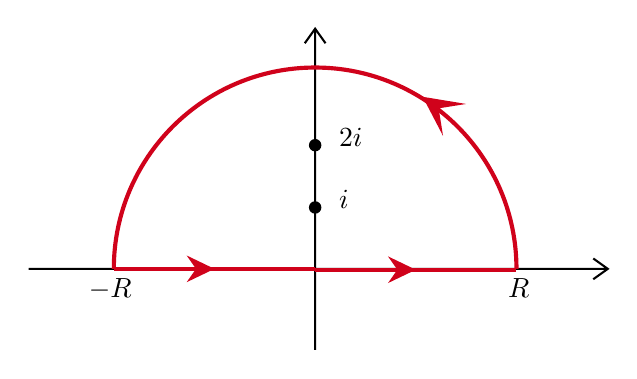
\begin{tikzpicture}[x=0.75pt,y=0.75pt,yscale=-1,xscale=1]
%uncomment if require: \path (0,181); %set diagram left start at 0, and has height of 181

%Shape: Axis 2D [id:dp663384449293001] 
\draw  (162.5,130.33) -- (441.5,130.33)(300.5,14.63) -- (300.5,169.33) (434.5,125.33) -- (441.5,130.33) -- (434.5,135.33) (295.5,21.63) -- (300.5,14.63) -- (305.5,21.63)  ;
%Straight Lines [id:da95452190554064] 
\draw [color={rgb, 255:red, 208; green, 2; blue, 27 }  ,draw opacity=1 ][line width=1.5]    (300.5,130.75) -- (397.5,130.75) ;
\draw [shift={(349,130.75)}, rotate = 180] [fill={rgb, 255:red, 208; green, 2; blue, 27 }  ,fill opacity=1 ][line width=0.08]  [draw opacity=0] (13.4,-6.43) -- (0,0) -- (13.4,6.44) -- (8.9,0) -- cycle    ;
%Shape: Arc [id:dp42287292414644995] 
\draw  [draw opacity=0][line width=1.5]  (203.5,130.33) .. controls (203.5,76.76) and (246.93,33.33) .. (300.5,33.33) .. controls (354.07,33.33) and (397.5,76.76) .. (397.5,130.33) -- (300.5,130.33) -- cycle ; \draw  [color={rgb, 255:red, 208; green, 2; blue, 27 }  ,draw opacity=1 ][line width=1.5]  (203.5,130.33) .. controls (203.5,76.76) and (246.93,33.33) .. (300.5,33.33) .. controls (354.07,33.33) and (397.5,76.76) .. (397.5,130.33) ;
%Straight Lines [id:da4448454277513003] 
\draw [color={rgb, 255:red, 208; green, 2; blue, 27 }  ,draw opacity=1 ][line width=1.5]    (203.5,130.33) -- (300.5,130.33) ;
\draw [shift={(252,130.33)}, rotate = 180] [fill={rgb, 255:red, 208; green, 2; blue, 27 }  ,fill opacity=1 ][line width=0.08]  [draw opacity=0] (13.4,-6.43) -- (0,0) -- (13.4,6.44) -- (8.9,0) -- cycle    ;
\draw  [draw opacity=0][fill={rgb, 255:red, 208; green, 2; blue, 27 }  ,fill opacity=1 ] (362.12,66.27) -- (352.31,47.43) -- (373.27,50.88) -- (360,53) -- cycle ;
%Shape: Circle [id:dp1636459542824935] 
\draw  [draw opacity=0][fill={rgb, 255:red, 0; green, 0; blue, 0 }  ,fill opacity=1 ] (297.5,100.75) .. controls (297.5,99.1) and (298.84,97.75) .. (300.5,97.75) .. controls (302.16,97.75) and (303.5,99.1) .. (303.5,100.75) .. controls (303.5,102.41) and (302.16,103.75) .. (300.5,103.75) .. controls (298.84,103.75) and (297.5,102.41) .. (297.5,100.75) -- cycle ;
%Shape: Circle [id:dp3693616304321441] 
\draw  [draw opacity=0][fill={rgb, 255:red, 0; green, 0; blue, 0 }  ,fill opacity=1 ] (297.5,70.75) .. controls (297.5,69.1) and (298.84,67.75) .. (300.5,67.75) .. controls (302.16,67.75) and (303.5,69.1) .. (303.5,70.75) .. controls (303.5,72.41) and (302.16,73.75) .. (300.5,73.75) .. controls (298.84,73.75) and (297.5,72.41) .. (297.5,70.75) -- cycle ;

% Text Node
\draw (392,133.4) node [anchor=north west][inner sep=0.75pt]    {$R$};
% Text Node
\draw (190,133.4) node [anchor=north west][inner sep=0.75pt]    {$-R$};
% Text Node
\draw (310.5,90.9) node [anchor=north west][inner sep=0.75pt]    {$i$};
% Text Node
\draw (310.5,60.9) node [anchor=north west][inner sep=0.75pt]    {$2i$};


\end{tikzpicture}
\end{figure}
\FloatBarrier

Notiamo che $| u( z)| \sim \frac{1}{z^{4}}$ per $| z| \rightarrow +\infty $. Per il teorema dei residui e il lemma di Jordan
\begin{equation*}
\begin{aligned}
\hat{u}( \xi ) & =\int ^{+\infty }_{-\infty }\frac{e^{-i\xi x}}{\left( 1+x^{2}\right)\left( 4+x^{2}\right)}\overset{\xi < 0}{=} 2\pi i\cdotp \{\mathrm{Res}( u,i) +\mathrm{Res}( u,2i)\}\\
 & =2\pi i\cdotp \left\{\frac{e^{\xi }}{6i} -\frac{e^{2\xi }}{12i}\right\} =\frac{\pi }{3} e^{\xi } -\frac{\pi }{6} e^{2\xi } \ \ ( \xi < 0)
\end{aligned}
\end{equation*}
$u( x)$ è pari, allora $\hat{u}( \xi )$ è pari e reale.

$\Rightarrow $ i valori per $\xi  >0$ si ottengono imponendo $\hat{u}( -\xi ) =\hat{u}( \xi )$.

$u\in L^{1}(\mathbb{R})$, allora la sua trasformata è continua.

$\Rightarrow $ il valore per $\xi =0$ si ottiene per continuità.
\begin{equation*}
\hat{u}( \xi ) =\frac{\pi }{3} e^{-| \xi | } -\frac{\pi }{6} e^{-2| \xi | } \ \ \ \ \forall \xi \in \mathbb{R}
\end{equation*}
A questo punto ricordiamo la proprietà della \textit{modulazione}
\begin{equation*}
u( x) e^{iax} \mapsto \hat{u}( \xi -a)
\end{equation*}
e che possiamo scrivere le identità
\begin{equation*}
\cos \vartheta =\frac{e^{i\vartheta } +e^{-i\vartheta }}{2} \ \ \ \ \sin \vartheta =\frac{e^{i\vartheta } -e^{-i\vartheta }}{2i}
\end{equation*}
in modo da far apparire il termine per usare la proprietà
\begin{equation*}
\begin{aligned}
\mathcal{F}( f( x) ,\xi ) & =\mathcal{F}\left(\frac{\sin x}{\left( 1+x^{2}\right)\left( 4+x^{2}\right)} ,\xi \right)\\
 & =\mathcal{F}\left(\frac{e^{ix} -e^{-ix}}{2i\left( 1+x^{2}\right)\left( 4+x^{2}\right)} ,\xi \right)\\
 & =\frac{1}{2i}\mathcal{F}\left(\frac{e^{ix}}{\left( 1+x^{2}\right)\left( 4+x^{2}\right)} ,\xi \right) +\frac{1}{2i}\mathcal{F}\left(\frac{-e^{-ix}}{\left( 1+x^{2}\right)\left( 4+x^{2}\right)} ,\xi \right)\\
 & =\frac{1}{2i}\left\{\mathcal{F}\left(\frac{1}{\left( 1+x^{2}\right)\left( 4+x^{2}\right)} ,\xi -1\right) -\mathcal{F}\left(\frac{1}{\left( 1+x^{2}\right)\left( 4+x^{2}\right)} ,\xi +1\right)\right\}\\
 & =\frac{1}{2i}\left\{\frac{\pi }{3} e^{-| \xi -1| } -\frac{\pi }{6} e^{-2| \xi -1| } -\frac{\pi }{3} e^{-| \xi +1| } +\frac{\pi }{6} e^{-2| \xi +1| }\right\}
\end{aligned}
\end{equation*}
\Soluzione

Conviene riscrivere $u$
\begin{equation*}
u( x) =\frac{2\cos x}{1+x^{2}} =u( x) =\frac{2\frac{e^{ix} +e^{-ix}}{2}}{1+x^{2}} =\frac{e^{ix} +e^{-ix}}{1+x^{2}}
\end{equation*}
Sappiamo dal primo esercizio che
\begin{equation*}
\mathcal{F}\left\{\frac{1}{1+x^{2}} ,\xi \right\} =\pi e^{-| \xi | }
\end{equation*}
Allora
\begin{equation*}
\begin{aligned}
\mathcal{F}\{u( x) ,\xi \} & =\mathcal{F}\left\{\frac{e^{ix} +e^{-ix}}{1+x^{2}} ,\xi \right\}\\
 & =\mathcal{F}\left\{\frac{e^{ix}}{1+x^{2}} ,\xi \right\} +\mathcal{F}\left\{\frac{e^{-ix}}{1+x^{2}} ,\xi \right\}\\
 & =\pi e^{-| \xi -1| } +\pi e^{-| \xi +1| }
\end{aligned}
\end{equation*}
\Soluzione

Posto
\begin{equation*}
g( x) =\frac{\cos( 2x)}{1+x^{2}}
\end{equation*}
Per definizione
\begin{equation*}
\hat{g}( \xi ) =\int _{\mathbb{R}} e^{-i\xi x} g( x) dx
\end{equation*}
e dunque
\begin{equation*}
f( \tau ) =\hat{g}\left( \tau ^{2} -2\right)
\end{equation*}
Sappiamo per il primo esercizio che
\begin{equation*}
\mathcal{F}\left\{\frac{1}{1+x^{2}} ,\xi \right\} =\pi e^{-| \xi | }
\end{equation*}
Inoltre
\begin{equation*}
g( x) =\frac{\cos( 2x)}{1+x^{2}} =\frac{e^{2ix} +e^{-2ix}}{2\left( 1+x^{2}\right)}
\end{equation*}
Allora
\begin{equation*}
\hat{g}( \xi ) =\mathcal{F}\{g( x) ,\xi \} =\frac{\pi }{2}\left( e^{-| \xi -2| } +e^{-| \xi +2| }\right)
\end{equation*}
E determiniamo $f( \tau )$ come
\begin{equation*}
f( \tau ) =\hat{g}\left( \tau ^{2} -2\right) =\frac{\pi }{2}\left( e^{-\left| \tau ^{2} -4\right| } +e^{-\left| \tau ^{2}\right| }\right)
\end{equation*}
\Soluzione
\begin{enumerate}
\item Calcoliamo\begin{equation*}
\begin{aligned}
\hat{f}( \xi ) & =\int _{\mathbb{R}} e^{-i\xi x} f( x) dx\\
 & =\int ^{0}_{-1} -e^{-i\xi x} dx+\int ^{1}_{0} e^{-i\xi x} dx\\
 & =\left[\frac{1}{i\xi } e^{-i\xi x}\right]^{0}_{-1} +\left[ -\frac{1}{i\xi } e^{-i\xi x}\right]^{1}_{0}\\
 & =\frac{1}{i\xi }\left( 1-e^{i\xi } -e^{-i\xi } +1\right)\\
 & =\frac{1}{i\xi }\left( 2-\textcolor[rgb]{0.29,0.56,0.89}{\left(e^{i\xi }+e^{-i\xi }\right)}\right) =\frac{1}{i\xi }( 2-\textcolor[rgb]{0.29,0.56,0.89}{2\cos\xi })
\end{aligned}
\end{equation*}
\item Calcoliamo\begin{equation*}
\hat{g}( \xi ) =i\frac{d}{d\xi }\hat{f}( \xi ) =i\frac{d}{d\xi }\frac{2-2\cos \xi }{i\xi } =\frac{2( 1-\cos \xi -\xi \sin \xi )}{\xi ^{2}}
\end{equation*}
\end{enumerate}
\Soluzione

$f$ può essere riscritta
\begin{equation*}
f( x) =\begin{cases}
1-x^{2} , & -1\leqslant x\leqslant 1\\
0, & \text{altrove}
\end{cases}
\end{equation*}
$f$ è pari, allora $\hat{f}$ è pari e reale.
\begin{equation*}
\hat{f}( \xi ) =\int _{\mathbb{R}} e^{-i\xi x} f( x) dx=\int ^{1}_{-1} e^{-i\xi x}\left( 1-x^{2}\right) dx=( *)
\end{equation*}
Usando l'analisi complessa
\begin{equation*}
\rho e^{i\vartheta } =\rho [\cos \vartheta +i\sin \vartheta ]
\end{equation*}
allora
\begin{align*}
( *) & =\int ^{1}_{-1}[\cos( \xi x) -i\sin( \xi x)]\left( 1-x^{2}\right) dx\\
 & =\int ^{1}_{-1}\underbrace{\cos( \xi x)\left( 1-x^{2}\right)}_{\text{pari}} dx-i\int ^{1}_{-1}\underbrace{\sin( \xi x)\left( 1-x^{2}\right)}_{\text{dispari}} dx\\
 & =2\int ^{1}_{0}\underbrace{\cos( \xi x)}_{g'}\underbrace{\left( 1-x^{2}\right)}_{f} -i\cdotp 0\\
 & \overset{\text{ipp}}{=} 2\left\{\cancel{\left[\left( 1-x^{2}\right)\frac{1}{\xi }\sin( 2\xi )\right]^{1}_{0}} -\int ^{1}_{0}\frac{-2x}{\xi }\sin( \xi x) dx\right\}\\
 & =\frac{4}{\xi }\int ^{1}_{0}\underbrace{x}_{f}\underbrace{\sin( \xi x)}_{g'} dx\\
 & \overset{\text{ipp}}{=}\frac{4}{\xi }\left\{\left[ -\frac{x}{\xi }\cos( \xi x)\right]^{1}_{0} -\int ^{1}_{0} -\frac{1}{\xi }\cos( \xi x) dx\right\}\\
 & =\frac{4}{\xi }\left\{-\frac{1}{\xi }\cos \xi +\left[\frac{1}{\xi ^{2}}\sin( \xi x)\right]^{1}_{0}\right\}\\
 & =\frac{4}{\xi }\left\{-\frac{1}{\xi }\cos \xi +\frac{1}{\xi ^{2}}\sin( \xi )\right\}\\
 & =-\frac{4}{\xi ^{2}}\cos \xi +\frac{4}{\xi ^{3}}\sin \xi =4\left(\frac{\sin \xi -\xi \cos \xi }{\xi ^{3}}\right)
\end{align*}
\begin{theorem}
[Antitrasformata di Fourier] Siano $u,\hat{u} \in L^{1}(\mathbb{R})$
\begin{equation*}
\boxed{u( x) =\frac{1}{2\pi }\int _{\mathbb{R}} e^{i\xi x}\hat{u}( \xi ) d\xi \ \ \forall x\in \mathbb{R}}
\end{equation*}
\end{theorem}
Allora, ricordando che $\hat{f}$ è pari
\begin{align*}
f( x) & =\frac{1}{2\pi }\int _{\mathbb{R}} e^{i\xi x}\hat{f}( \xi ) d\xi \\
 & =\frac{1}{2\pi }\int _{\mathbb{R}}[\cos( \xi x) +i\sin( \xi x)]\hat{f}( \xi ) \xi \\
 & =\frac{1}{2\pi }\int _{\mathbb{R}}\cos( \xi x) \cdotp \hat{f}( \xi ) d\xi \\
 & =\frac{1}{2\pi } \cdotp 2\int ^{\infty }_{0}\cos( \xi x) \cdotp \hat{f}( \xi ) d\xi \\
 & =\frac{1}{2\pi } \cdotp 2\int ^{\infty }_{0}\cos( \xi x) \cdotp 4\left(\frac{\sin \xi -\xi \cos \xi }{\xi ^{3}}\right) d\xi \\
 & =\frac{4}{\pi }\int ^{+\infty }_{0}\frac{\sin \xi -\xi \cos \xi }{\xi ^{3}}\cos( \xi x) d\xi 
\end{align*}
Per avere l'integrale richiesto dobbiamo prendere $x=\frac{1}{2}$
\begin{equation*}
f\left(\frac{1}{2}\right) =\frac{4}{\pi }\int ^{+\infty }_{0}\frac{\sin \xi -\xi \cos \xi }{\xi ^{3}}\cos\left(\frac{\xi }{2}\right) d\xi \ \ \ \ \ \ \ \ f\left(\frac{1}{2}\right) =1-\frac{1}{4} =\frac{3}{4}
\end{equation*}
Troviamo quindi il l'integrale richiesto, a meno di un segno
\begin{equation*}
\int ^{+\infty }_{0}\frac{x\cos x-\sin x}{x^{3}}\cos\left(\frac{x}{2}\right) dx=-\frac{3}{4} \cdotp \frac{\pi }{4} =-\frac{3\pi }{16}
\end{equation*}
\chapter{Esercitazione 9 - Boella}
\ParteEsercizi

Richiami di teoria sulla Trasformata di Laplace.
\begin{definition}
[Funzione di Heaviside] Si definisce
\begin{equation*}
H( t) =\begin{cases}
1, & t\geqslant 0\\
0, & t< 0
\end{cases}
\end{equation*}
\end{definition}
\begin{figure}[htpb]
	\centering
\tikzset{every picture/.style={line width=0.75pt}} %set default line width to 0.75pt        

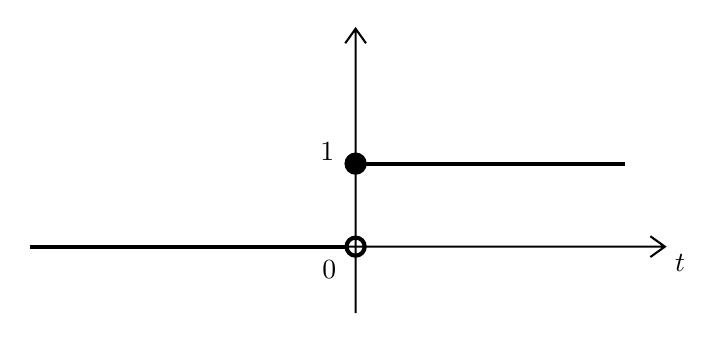
\begin{tikzpicture}[x=0.75pt,y=0.75pt,yscale=-1,xscale=1]
%uncomment if require: \path (0,158); %set diagram left start at 0, and has height of 158

%Shape: Axis 2D [id:dp10122351594887924] 
\draw  (150.5,120) -- (448.5,120)(299.5,15) -- (299.5,152) (441.5,115) -- (448.5,120) -- (441.5,125) (294.5,22) -- (299.5,15) -- (304.5,22)  ;
%Straight Lines [id:da9543821452612189] 
\draw [line width=1.5]    (142.5,120) -- (296.15,120) ;
\draw [shift={(299.5,120)}, rotate = 0] [color={rgb, 255:red, 0; green, 0; blue, 0 }  ][line width=1.5]      (0, 0) circle [x radius= 4.36, y radius= 4.36]   ;
%Straight Lines [id:da289644330277681] 
\draw [line width=1.5]    (429.5,80) -- (299.5,80) ;
\draw [shift={(299.5,80)}, rotate = 180] [color={rgb, 255:red, 0; green, 0; blue, 0 }  ][fill={rgb, 255:red, 0; green, 0; blue, 0 }  ][line width=1.5]      (0, 0) circle [x radius= 4.36, y radius= 4.36]   ;

% Text Node
\draw (281,68.4) node [anchor=north west][inner sep=0.75pt]    {$1$};
% Text Node
\draw (282,125.4) node [anchor=north west][inner sep=0.75pt]    {$0$};
% Text Node
\draw (452,122.4) node [anchor=north west][inner sep=0.75pt]    {$t$};


\end{tikzpicture}
\end{figure}
\FloatBarrier
Diciamo che $\mathcal{L}\{f( t)\} =F( s)$.

\textbf{Alcune trasformate notevoli.}
\begin{itemize}
\item $\mathcal{L}\{H( t)\} =\int ^{+\infty }_{0} e^{-st} dt=\frac{1}{s}$, in questo caso $\lambda =0$
\item $\mathcal{L}\left\{t^{k} f( t)\right\} =( -1)^{k}\frac{d^{k}}{ds^{k}} F( s)$
\item $\mathcal{L}\{tH( t)\} =\frac{1}{s^{2}}$

$\mathcal{L}\left\{t^{2} H( t)\right\} =-\left( -\frac{2}{s^{3}}\right) =\frac{2}{s^{3}}$

$\mathcal{L}\left\{t^{3} H( t)\right\} =-\frac{d}{ds}\left(\frac{2}{s^{3}}\right) =\frac{6}{s^{4}}$

$\mathcal{L}\left\{t^{n} H( t)\right\} =\frac{n!}{s^{n+1}}$
\item $\Gamma ( x) =\int ^{+\infty }_{0} t^{x-1} e^{-t} dt$
\begin{itemize}
\item $\Gamma ( n) =( n-1) !$ se $n$ è intero
\item $\Gamma ( x+1) =x\Gamma ( x)$ per ogni $x >0$
\item $\Gamma \left(\frac{1}{2}\right) =\sqrt{\pi }$
\end{itemize}

$\mathcal{L}\left\{t^{\alpha } H( t)\right\} =\frac{\Gamma ( \alpha +1)}{s^{\alpha +1}}$ se $\mathrm{Re}( \alpha )  >-1$
\item $\mathcal{L}\left\{\frac{1}{\sqrt{t}} H( t)\right\} =\frac{\Gamma \left(\frac{1}{2}\right)}{\sqrt{s}} =\frac{\sqrt{\pi }}{\sqrt{s}}$
\end{itemize}

\textbf{Proprietà.}
\begin{itemize}
\item $\mathcal{L}\{f( \alpha t)\} =\frac{1}{\alpha } F\left(\frac{s}{\alpha }\right)$
\item $\mathcal{L}\{f( t-\alpha )\} =e^{-\alpha s} F( s)$
\item $\mathcal{L}\left\{e^{\alpha t} f( t)\right\} =F( s-\alpha )$
\item $\mathcal{L}\{f'( t)\} =sF( s) -f\left( 0^{+}\right)$
\item $\mathcal{L}\{f''( t)\} =s^{2} F( s) -sf\left( 0^{+}\right) -f'\left( 0^{+}\right)$
\item $\mathcal{L}\left\{\int ^{t}_{0} f( \tau ) d\tau \right\} =\frac{1}{s} F( s)$
\item $\mathcal{L}\left\{\frac{1}{t} f( t)\right\} =\int ^{+\infty }_{s} F( \sigma ) d\sigma $
\end{itemize}

\textbf{Altre trasformate notevoli.}
\begin{itemize}
\item $\mathcal{L}\left\{e^{\alpha t} H( t)\right\} =\frac{1}{s-\alpha }$
\item $\mathcal{L}\{\sin( \omega t) H( t)\} =\frac{\omega }{s^{2} +\omega ^{2}}$, pari in $s$
\item $\mathcal{L}\{\cos( \omega t) H( t)\} =\frac{s}{s^{2} +\omega ^{2}}$, dispari in $s$
\item $\mathcal{L}\{\sinh( \omega t) H( t)\} =\frac{\omega }{s^{2} -\omega ^{2}}$
\item $\mathcal{L}\{\cosh( \omega t) H( t)\} =\frac{s}{s^{2} -\omega ^{2}}$
\end{itemize}
\Esercizio{}

Calcolare
\begin{equation*}
\mathcal{L}\left\{e^{-\alpha t}\sin( \omega t) H( t)\right\} =\frac{\omega }{\omega ^{2} +( s+\alpha )^{2}}
\end{equation*}
Calcolare
\begin{equation*}
\begin{aligned}
\mathcal{L}\left\{e^{-t}\sin^{2}( t) H( t)\right\} & =\frac{1}{2}\mathcal{L}\left\{e^{-t}( 1-\cos 2t) H( t)\right\} =\frac{1}{2}\left[\frac{1}{s+1} -\frac{s+1}{4+( s+1)^{2}}\right]\\
 & =\frac{1}{2}\frac{4}{( s+1)\left( 4+( s+1)^{2}\right)} =\frac{2}{( s+1)\left( 4+( s+1)^{2}\right)}
\end{aligned}
\end{equation*}
Calcolare
\begin{equation*}
\mathcal{L}\left\{\int ^{t}_{0}\sin( 2\tau ) d\tau \right\} =\frac{2}{s\left( 4+s^{2}\right)}
\end{equation*}
Calcolare
\begin{equation*}
\begin{aligned}
\mathcal{L}\left\{t^{2} e^{2t} H( t)\right\} & =\mathcal{L}\left\{e^{2t}\left[ t^{2} H( t)\right]\right\} =\frac{2}{( s-2)^{3}}\\
 & =\mathcal{L}\left\{t^{2}\left[ e^{2t} H( t)\right]\right\} =\frac{d^{2}}{ds^{2}}\frac{1}{s-2} =\frac{2}{( s-2)^{3}} \ 
\end{aligned}
\end{equation*}
Calcolare
\begin{equation*}
\begin{aligned}
\mathcal{L}\left\{\frac{\sin t}{t} H( t)\right\} & =\mathcal{L}\left\{\frac{1}{t}[\sin( t) H( t)]\right\} =\int ^{+\infty }_{s}\frac{1}{1+\sigma ^{2}} d\sigma \\
 & =[\arctan \sigma ]^{+\infty }_{s} =\frac{\pi }{2} -\arctan s
\end{aligned}
\end{equation*}
\Esercizio{}

Sia
\begin{equation*}
f( t) =\begin{cases}
t, & 0< t< 2\\
4-t, & 2\leqslant t< 4\\
0, & \text{altrimenti}
\end{cases}
\end{equation*}


\begin{figure}[htpb]
	\centering
\tikzset{every picture/.style={line width=0.75pt}} %set default line width to 0.75pt        

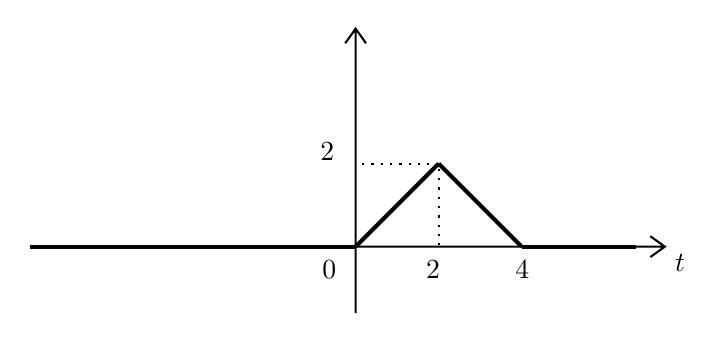
\begin{tikzpicture}[x=0.75pt,y=0.75pt,yscale=-1,xscale=1]
%uncomment if require: \path (0,156); %set diagram left start at 0, and has height of 156

%Shape: Axis 2D [id:dp387811944250509] 
\draw  (150.5,110) -- (448.5,110)(299.5,5) -- (299.5,142) (441.5,105) -- (448.5,110) -- (441.5,115) (294.5,12) -- (299.5,5) -- (304.5,12)  ;
%Straight Lines [id:da44163391987628864] 
\draw [line width=1.5]    (142.5,110) -- (299.5,110) ;
%Straight Lines [id:da9344407308358857] 
\draw [line width=1.5]    (434.5,110) -- (379.5,110) ;
%Straight Lines [id:da9599366268835559] 
\draw [line width=1.5]    (339.5,70) -- (299.5,110) ;
%Straight Lines [id:da4331170712538084] 
\draw [line width=1.5]    (379.5,110) -- (339.5,70) ;
%Straight Lines [id:da332148534363488] 
\draw [line width=0.75]  [dash pattern={on 0.84pt off 2.51pt}]  (339.5,70) -- (299.5,70) ;
%Straight Lines [id:da8792189758357065] 
\draw [line width=0.75]  [dash pattern={on 0.84pt off 2.51pt}]  (339.5,109.39) -- (339.5,70) ;

% Text Node
\draw (281,58.4) node [anchor=north west][inner sep=0.75pt]    {$2$};
% Text Node
\draw (282,115.4) node [anchor=north west][inner sep=0.75pt]    {$0$};
% Text Node
\draw (452,112.4) node [anchor=north west][inner sep=0.75pt]    {$t$};
% Text Node
\draw (332,115.4) node [anchor=north west][inner sep=0.75pt]    {$2$};
% Text Node
\draw (375,115.4) node [anchor=north west][inner sep=0.75pt]    {$4$};


\end{tikzpicture}
\end{figure}
\FloatBarrier

Scriviamo diversamente la $f$
\begin{equation*}
\begin{aligned}
f( t) & =t[ H( t) -H( t-2)] +( 4-t)[ H( t-2) -H( t-4)]\\
 & =tH( t) -2( t-2) H( t-2) +( t-4) H( t-4)\\
 & \\
 & \Rightarrow \ \ \mathcal{L}\{f( t)\} =\frac{1}{s^{2}} -2\frac{e^{-2s}}{s^{2}} +\frac{e^{-4s}}{s^{2}}
\end{aligned}
\end{equation*}
\Esercizio{}

Sia
\begin{equation*}
g( t) =\begin{cases}
t, & 0< t< 1\\
2-t, & 1\leqslant t< 2\\
t-2, & 2\leqslant t
\end{cases}
\end{equation*}


\begin{figure}[htpb]
	\centering
\tikzset{every picture/.style={line width=0.75pt}} %set default line width to 0.75pt        

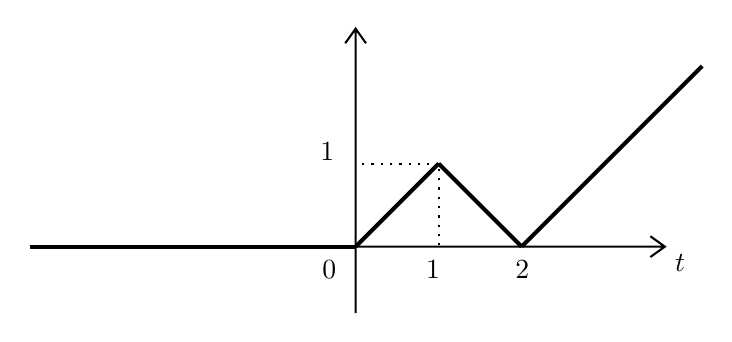
\begin{tikzpicture}[x=0.75pt,y=0.75pt,yscale=-1,xscale=1]
%uncomment if require: \path (0,156); %set diagram left start at 0, and has height of 156

%Shape: Axis 2D [id:dp16516737574733087] 
\draw  (150.5,110) -- (448.5,110)(299.5,5) -- (299.5,142) (441.5,105) -- (448.5,110) -- (441.5,115) (294.5,12) -- (299.5,5) -- (304.5,12)  ;
%Straight Lines [id:da9317289947100813] 
\draw [line width=1.5]    (142.5,110) -- (299.5,110) ;
%Straight Lines [id:da695102507830573] 
\draw [line width=1.5]    (466.48,23.02) -- (379.5,110) ;
%Straight Lines [id:da44710495183723054] 
\draw [line width=1.5]    (339.5,70) -- (299.5,110) ;
%Straight Lines [id:da5381477224930931] 
\draw [line width=1.5]    (379.5,110) -- (339.5,70) ;
%Straight Lines [id:da018036722756767043] 
\draw [line width=0.75]  [dash pattern={on 0.84pt off 2.51pt}]  (339.5,70) -- (299.5,70) ;
%Straight Lines [id:da9481675028243701] 
\draw [line width=0.75]  [dash pattern={on 0.84pt off 2.51pt}]  (339.5,109.39) -- (339.5,70) ;

% Text Node
\draw (281,58.4) node [anchor=north west][inner sep=0.75pt]    {$1$};
% Text Node
\draw (282,115.4) node [anchor=north west][inner sep=0.75pt]    {$0$};
% Text Node
\draw (452,112.4) node [anchor=north west][inner sep=0.75pt]    {$t$};
% Text Node
\draw (332,115.4) node [anchor=north west][inner sep=0.75pt]    {$1$};
% Text Node
\draw (375,115.4) node [anchor=north west][inner sep=0.75pt]    {$2$};


\end{tikzpicture}
\end{figure}
\FloatBarrier

Scriviamo diversamente la $g$
\begin{equation*}
\begin{aligned}
g( t) & =t[ H( t) -H( t-1)] +( 2-t)[ H( t-1) -H( t-2)] +( t-2)[ H( t-2)\\
 & \\
 & \Rightarrow \ \ \mathcal{L}\{g( t)\} =\frac{1}{s^{2}} -2\frac{e^{-s}}{s^{2}} +2\frac{e^{-2s}}{s^{2}}
\end{aligned}
\end{equation*}
\Esercizio{}

Calcolare l'antitrasformata
\begin{equation*}
\mathcal{L}^{-1}\left\{\frac{2s^{2} -4}{( s+1)( s-2)( s-3)}\right\} =\mathcal{L}^{-1}\{( *)\}
\end{equation*}
Scomponiamo in fratti semplici
\begin{equation*}
\begin{aligned}
( *) & =\frac{A}{s+1} +\frac{B}{s-2} +\frac{C}{s-3}\\
 & =\frac{A( s-2)( s-3) +B( s+1)( s-3) +C( s+1)( s-2)}{( s+1)( s-2)( s-3)}\\
 & \Rightarrow \ \ A=-\frac{1}{6} \ \ \ \ B=-\frac{3}{8} \ \ \ \ C=\frac{7}{2}
\end{aligned}
\end{equation*}
Quindi
\begin{equation*}
\begin{aligned}
\mathcal{L}^{-1}\{( *)\} & =\mathcal{L}^{-1}\left\{-\frac{1}{6}\frac{1}{s+1} -\frac{3}{8}\frac{1}{s-2} +\frac{7}{2}\frac{1}{s-3}\right\}\\
 & =\left[ -\frac{1}{6} e^{-t} -\frac{3}{8} e^{2t} +\frac{7}{2} e^{3t}\right] H( t)
\end{aligned}
\end{equation*}
\Esercizio{}

Calcolare l'antitrasformata
\begin{equation*}
\mathcal{L}^{-1}\left\{\frac{3s+1}{( s-1)\left( s^{2} +1\right)}\right\} =\mathcal{L}^{-1}\{( *)\}
\end{equation*}
Scomponiamo in fratti semplici
\begin{equation*}
\begin{aligned}
( *) & =\frac{A}{s-1} +\frac{Bs+C}{\left( s^{2} +1\right)}\\
 & =\frac{A\left( s^{2} +1\right) +( Bs+C)( s-1)}{( s-1)\left( s^{2} +1\right)}\\
 & \Rightarrow \ \ A=2\ \ \ \ C=1\ \ \ \ B=-2
\end{aligned}
\end{equation*}
Quindi
\begin{equation*}
\begin{aligned}
\mathcal{L}^{-1}\{( *)\} & =\mathcal{L}^{-1}\left\{\frac{2}{s-1} +\frac{-2s+1}{s^{2} +1}\right\}\\
 & =\mathcal{L}^{-1}\left\{\frac{2}{s-1} -\frac{2s}{s^{2} +1} +\frac{1}{s^{2} +1}\right\}\\
 & =\left[ 2e^{t} +\sin t-2\cos t\right] H( t)
\end{aligned}
\end{equation*}
\Esercizio{}

Calcolare
\begin{equation*}
\mathcal{L}^{-1}\left\{\frac{1}{( s+3)^{2}}\right\} =e^{-3t} tH( t)
\end{equation*}
Calcolare
\begin{equation*}
\begin{aligned}
\mathcal{L}^{-1}\left\{\frac{e^{-2s}}{s^{3} +s}\right\} & =\mathcal{L}^{-1}\left\{\frac{1}{s}\frac{e^{-2s}}{s^{2} +1}\right\}\\
 & =\int ^{t}_{0}\sin( \tau -2) H( \tau -2) d\tau \\
 & =H( t-2)\int ^{t}_{2}\sin( \tau -2) d\tau \\
 & =H( t-2)[ -\cos( \tau -2)]^{t}_{2}\\
 & =H( t-2)[ 1-\cos( t-2)]
\end{aligned}
\end{equation*}
Calcolare
\begin{equation*}
\begin{aligned}
\mathcal{L}^{-1}\left\{\frac{4e^{-2s}\sinh s}{s^{2} +4}\right\} & =\mathcal{L}^{-1}\left\{\frac{2\left( e^{-s} -e^{-3s}\right)}{s^{2} +4}\right\}\\
 & =\sin[ 2( t-1)] H( t-1) -\sin[ 2( t-3)] H( t-3)
\end{aligned}
\end{equation*}
\Esercizio{}

Determinare le soluzioni $u\in L^{1}(\mathbb{R})$ di
\begin{equation*}
u'-\alpha u=e^{-\alpha x} H( x) \ \ \ \ \alpha  >0
\end{equation*}
\Esercizio{}

Risolvere
\begin{equation*}
u''+2xu'+2u=0
\end{equation*}
\Esercizio{}

Determinare le soluzioni $u\in L^{1}(\mathbb{R})$ di
\begin{equation*}
xu''+2u'-xu=xe^{-| x| }
\end{equation*}
\ParteSoluzioni
\Soluzione

Soluzione nella parte esercizi.
\Soluzione

Soluzione nella parte esercizi.
\Soluzione

Soluzione nella parte esercizi.
\Soluzione

Soluzione nella parte esercizi.
\Soluzione

Soluzione nella parte esercizi.
\Soluzione

Soluzione nella parte esercizi.
\Soluzione

\underline{\textbf{Con l'Analisi 2.}}
\begin{theorem}
Ricordiamo questo risultato di Analisi 2.
\begin{equation*}
y'-\alpha y=f
\end{equation*}
L'integrale generale è
\begin{equation*}
y( x) =Ce^{\alpha x} +y^{\star }( x)
\end{equation*}
\end{theorem}
Nel nostro caso
\begin{equation*}
f( x) =\begin{cases}
0, & x< 0\\
e^{-\alpha x} , & x\geqslant 0
\end{cases}
\end{equation*}
Quindi come equazione particolare
\begin{equation*}
y^{\star }( x) =\begin{cases}
0, & x< 0\\
Ae^{-\alpha x} =-\frac{1}{2\alpha } e^{-\alpha x} , & x\geqslant 0
\end{cases}
\end{equation*}
Quindi l'integrale generale è
\begin{equation*}
\begin{aligned}
y( x) & =\begin{cases}
C_{1} e^{\alpha x} , & x< 0\\
C_{2} e^{\alpha x} -\frac{1}{2\alpha } e^{-\alpha x} , & x\geqslant 0
\end{cases} & C_{1} =C_{2} -\frac{1}{2\alpha }\\
 & =\begin{cases}
Ce^{\alpha x} , & x< 0\\
\left( C+\frac{1}{2\alpha }\right) e^{\alpha x} -\frac{1}{2\alpha } e^{-\alpha x} , & x\geqslant 0
\end{cases} & 
\end{aligned}
\end{equation*}
\underline{\textbf{Con Fourier.}}

Trasformiamo secondo Fourier
\begin{equation*}
\begin{aligned}
\mathcal{F}\left\{e^{-\alpha x} H( x)\right\} & =\int ^{+\infty }_{0} e^{-i\xi x} e^{-\alpha x} dx=\int ^{+\infty }_{0} e^{-( \alpha +i\xi ) x} dx\\
 & =\left[ -\frac{1}{\alpha +i\xi } e^{-( \alpha +i\xi ) x}\right]^{+\infty }_{0} =\frac{1}{\alpha +i\xi }
\end{aligned}
\end{equation*}
Torniamo all'equazione
\begin{equation*}
\begin{aligned}
i\xi \hat{u} -\alpha \hat{u} =\frac{1}{\alpha +i\xi } \ \  & \Rightarrow \ \ ( i\xi -\alpha )\hat{u} =\frac{1}{\alpha +i\xi }\\
 & \Rightarrow \ \ \hat{u} =-\frac{1}{\alpha -i\xi } \cdotp \frac{1}{\alpha +i\xi } =-\frac{1}{\alpha ^{2} +\xi ^{2}}
\end{aligned}
\end{equation*}
Ci ricordiamo che
\begin{equation*}
\mathcal{F}\left\{e^{-\alpha | x| }\right\} =\frac{2\alpha }{\alpha ^{2} +\xi ^{2}} \ \ \Rightarrow \ \ u( x) =-\frac{1}{2\alpha } e^{-\alpha | x| }
\end{equation*}
Ma quelle trovate con l'Analisi 2 dove sono finite?
\begin{equation*}
y( x) \notin L^{1} \ \text{se} \ \left( C+\frac{1}{2\alpha }\right) \neq 0
\end{equation*}
Con Fourier richiediamo che stiano in $L^{1}$ e l'esponenziale positivo causa problemi, quindi per trovare, tra le infinite soluzioni, quella secondo Fourier, dobbiamo porre
\begin{equation*}
C+\frac{1}{2\alpha } =0\ \ \Rightarrow \ \ u( x) =-\frac{1}{2\alpha } e^{-| x| }
\end{equation*}
\Soluzione

È un'equazione lineare del II ordine omogenea, ma \textit{\underline{non a coefficienti costanti}}.
\begin{itemize}
\item $\mathcal{F}\{u\} =\hat{u}$
\item $\mathcal{F}\{u''\} =-\xi ^{2}\hat{u}$
\item $\mathcal{F}\{xu'\} =i\frac{d}{d\xi }\mathcal{F}\{u'\} =i\frac{d}{d\xi }( i\xi \hat{u}) =-(\hat{u} +\xi \hat{u} ')$
\end{itemize}

Allora
\begin{equation*}
\begin{array}{ l }
\Rightarrow \ \ -\xi ^{2}\hat{u} -2\left(\cancel{\hat{u}} +\xi \hat{u} '\right) +\cancel{2\hat{u}} =0\ \ \Rightarrow \ \ 2\xi \hat{u} '+\xi ^{2}\hat{u} =0\\
\Rightarrow \ \ \hat{u} '+\frac{\xi }{2}\hat{u} =0\ \ \Rightarrow \ \ \hat{u}( \xi ) =Ce^{-\frac{\xi ^{2}}{4}}
\end{array}
\end{equation*}
ma
\begin{equation*}
\mathcal{F}\left\{e^{-x^{2}}\right\} =\sqrt{\pi } e^{-\frac{\xi ^{2}}{4}} \ \ \Rightarrow \ \ u( x) =De^{-x^{2}}
\end{equation*}
$u( x)$ dovrebbe essere la combinazione lineare di due integrali particolari, qui abbiamo trovato solo quello che sta in $L^{1}$.
\Soluzione

Trasformiamo
\begin{itemize}
\item $\mathcal{F}\{xu''\} =i\frac{d}{d\xi }\left( -\xi ^{2}\hat{u}\right) =i\left( -2\xi \hat{u} -\xi ^{2}\hat{u} '\right)$
\item $\mathcal{F}\{u'\} =i\xi \hat{u}$
\item $\mathcal{F}\{xu\} =i\hat{u} '$
\item $\mathcal{F}\left\{xe^{-| x| }\right\} =i\frac{d}{d\xi }\frac{2}{1+\xi ^{2}} =i\cdotp \left[\frac{-4\xi }{\left( 1+\xi ^{2}\right)^{2}}\right]$
\end{itemize}

Allora
\begin{equation*}
\begin{aligned}
\cancel{-2i\xi \hat{u}} -i\xi ^{2}\hat{u} '+\cancel{2i\xi \hat{u}} -i\hat{u} ' & =-i\frac{4\xi }{\left( 1+\xi ^{2}\right)^{2}}\\
\left( 1+\xi ^{2}\right)\hat{u} ' & =\frac{4\xi }{\left( 1+\xi ^{2}\right)^{2}}\\
\hat{u} ' & =\frac{4\xi }{\left( 1+\xi ^{2}\right)^{3}} \ \ \Rightarrow \ \ \hat{u}( \xi ) =-\frac{1}{\left( 1+\xi ^{2}\right)^{2}} +c
\end{aligned}
\end{equation*}
dove $c=0$ perché altrimenti non è infinitesima all'infinito e non è la trasformata di alcuna funzione $L^{1}$.

$\hat{u}$ è pari, quindi $u$ è pari.
\chapter{Esercitazione 9 - Potrich}
\ParteEsercizi
\Esercizio{}

Sia
\begin{equation*}
f( x) =H( x) e^{-2x} =\begin{cases}
e^{-2x} , & x\geqslant 0\\
0, & x< 0
\end{cases}
\end{equation*}
calcolare $\displaystyle f*f$ e la sua trasformata di Fourier $\displaystyle \mathcal{F}( f*f)$.
\begin{nb}
[Prodotto di Convoluzione] È definito da
\begin{equation*}
( u*v)( x) =\int _{\mathbb{R}} u( x-y) v( y) dy=\int _{\mathbb{R}} u( y) v( x-y) dy
\end{equation*}
\end{nb}
\Esercizio{}

Determinare la trasformata di Fourier di
\begin{equation*}
f( x) =\ \left( 1-x^{2}\right) H\left( 1-x^{2}\right)
\end{equation*}
Ultilizzando il risultato ottenuto calcolare
\begin{equation*}
I=\int ^{+\infty }_{0}\frac{( x\cos x-\sin x)^{2}}{x^{6}} dx
\end{equation*}
\Esercizio{}
\begin{enumerate}
\item Calcolare la trasformata di Fourier delle funzioni:\begin{equation*}
f_{1}( x) =\frac{1}{1+x^{2}} \ \ \ \ f_{2}( x) =\frac{x}{\left( 1+x^{2}\right)^{2}}
\end{equation*}
\item Considerare la funzione:\begin{equation*}
f_{0}( x) =\arctan\left(\frac{1}{x}\right)
\end{equation*}

Stabilire se $\displaystyle f_{0} \in L^{1}(\mathbb{R})$ e/o se $\displaystyle f_{0} \in L^{2}(\mathbb{R})$.
\item Calcolare la derivata di $\displaystyle f_{0}$ nel senso delle distribuzioni.
\item Calcolare $\mathcal{F}\{f'_{0}\}$ e $\mathcal{F}\{f_{0}\}$.
\end{enumerate}
\Esercizio{}
\begin{definition}
Sia $\displaystyle f:\mathbb{R} \ \rightarrow \mathbb{C}$ si dice Laplace-trasformabile se:
\begin{equation*}
\mathrm{supp} f\subset [ 0,+\infty ) \ \ \ \ \land \ \ \ \ \exists \lambda \in \mathbb{R} :e^{-\lambda t} f( t) \in L^{1}(\mathbb{R})
\end{equation*}
\end{definition}
\begin{definition}
Si dice Ascissa di convergenza di $\displaystyle f$:
\begin{equation*}
\lambda _{f} :=\inf\left\{\lambda \in \mathbb{R} :e^{-\lambda t} f( t) \in L^{1}(\mathbb{R})\right\}
\end{equation*}
\end{definition}
\begin{definition}
Sia $\displaystyle f$ una funzione Laplace-trasformabile, allora la funzione:
\begin{equation*}
\boxed{F( s) :=\int ^{+\infty }_{0} e^{-st} f( t) dt\ \ \ \ \forall s\in \mathbb{C} :\mathrm{Re}( s)  >\lambda _{f}}
\end{equation*}
si dice Trasformata di Laplace di $\displaystyle f$.
\end{definition}
\begin{nb}
[Trasformate di Laplace notevoli] Si ha
\begin{equation*}
\mathcal{L}\{H( t)\} =\frac{1}{s} \ \ \ \ \forall s\in \mathbb{C} :\mathrm{Re}( s)  >\lambda _{f} =0
\end{equation*}
\end{nb}
\begin{theorem}
[Proprietà] Valgono
\begin{itemize}
\item Riscalamento\begin{equation*}
\mathcal{L}\{f( at)\} =\frac{1}{a} F\left(\frac{s}{a}\right) \ \ \ \ \mathrm{Re}( s)  >a\lambda _{f}
\end{equation*}
\item Ritardo\begin{equation*}
\mathcal{L}\{f( t-a)\} =e^{-as} F( s) \ \ \ \ \mathrm{Re}( s)  >\lambda _{f}
\end{equation*}
\item Prodotto con esponenziale\begin{equation*}
\mathcal{L}\left\{e^{at} f( t)\right\} =F( s-a) \ \ \ \ \mathrm{Re}( s)  >\lambda _{f} +\mathrm{Re}( a)
\end{equation*}
\item Linearità\begin{equation*}
\mathcal{L}\{af+bg\} =a\mathcal{L}\{f\} +b\mathcal{L}\{g\} \ \ \ \ \forall a,b\in \mathbb{C} ,\forall s:\mathrm{Re}( s)  >\max\{\lambda _{f} ,\lambda _{g}\}
\end{equation*}
\item Derivata della trasformata\begin{equation*}
\frac{d^{n}}{ds^{n}} F( s) =\mathcal{L}\left\{( -t)^{n} f( t)\right\}
\end{equation*}
\item La primitiva di una funzione $\mathcal{L}$-trasformabile è anch'essa una funzione $\mathcal{L}$-trasformabile\begin{equation*}
\mathcal{L}\left\{\int ^{t}_{0} f( \tau ) d\tau \right\} =\frac{1}{s}\mathcal{L}\{f( t)\} \ \ \ \ \forall s\in \mathbb{C} :\mathrm{Re}( s)  >\max\{\lambda _{f} ,0\}
\end{equation*}
\end{itemize}
\end{theorem}
Detta $\displaystyle H( x)$ la funzione di Heaviside, calcolare la trasformata di Laplace della funzione
\begin{equation*}
f( t) =H( t-1) te^{2t}
\end{equation*}
precisando l'ascissa di convergenza.
\Esercizio{}

Calcolare la trasformata di Laplace di
\begin{equation*}
f( t) =H( t)\sum ^{m}_{k=0} a_{k} t^{k} \ \ \ \ a_{k} \in \mathbb{R}
\end{equation*}
$\displaystyle \lambda _{f} =0$, perché se moltiplichiamo $\displaystyle f$ per $\displaystyle e^{-\lambda t}$ con $\displaystyle \lambda  >0$ le $\displaystyle f$ sono integrabili, 

mentre con $\displaystyle \lambda \leqslant 0$ non lo sono.
\Esercizio{}

Stabilire per quali valori di $\displaystyle a\in \mathbb{R}$ la funzione
\begin{equation*}
f_{a}( x) =H( x) e^{ax^{2} +2x}\sin^{2}( x)
\end{equation*}
è Laplace-trasformabile.

Calcolare poi la trasformata di Laplace di $\displaystyle f_{0}( x)$.
\Esercizio{}

Calcolare la trasformata di Laplace di
\begin{equation*}
f( t) =H( t)\sin( \omega t)
\end{equation*}
studiandone in particolare le trasformate di Laplace per $\displaystyle \omega =1$ e dedurre le antitrasformate di Laplace delle seguenti funzioni:
\begin{equation*}
J( s) =\frac{1}{\left( 1+s^{2}\right)^{2}} \ \ \ \ G( s) =\frac{s}{\left( 1+s^{2}\right)^{2}} \ \ \ \ K( s) =\frac{1}{s\left( s^{2} +4\right)}
\end{equation*}
\ParteSoluzioni
\Soluzione

Se $x< 0$
\begin{equation*}
( f*f)( x) =0
\end{equation*}
Se $x\geqslant 0$ ricordando che l'integrale è non nullo per 
\begin{equation*}
x-y\geqslant 0\ \ \land \ \ x\geqslant 0\ \ \ \ \Leftrightarrow \ \ \ \ y\leqslant x\ \ \land \ \ x\geqslant 0
\end{equation*}
quindi
\begin{align*}
( f*f)( x) & =\int _{\mathbb{R}} f( x-y) f( x) dy=\int ^{x}_{0} e^{-2( x-y)} e^{-2y} dy\\
 & =\int ^{x}_{0} e^{-2x} \ dy=e^{-2x}\int ^{x}_{0} dy=xe^{-2x}
\end{align*}
\begin{theorem}
Date $\displaystyle u,v\in \mathcal{S}(\mathbb{R}) \Rightarrow \ \widehat{u*v} =\hat{u} \cdot \hat{v}$.
\end{theorem}
\begin{align*}
\hat{f}( \xi ) & =\int _{\mathbb{R}} e^{-i\xi x} f( x) dx=\int _{\mathbb{R}} e^{-i\xi x} H( x) e^{-2x} dx=\int ^{+\infty }_{0} e^{-i\xi x} e^{-2x} dx\\
 & =\int ^{+\infty }_{0} e^{-x( i\xi +2)} dx=\left[ -\frac{e^{-x( i\xi +2)}}{i\xi +2}\right]^{+\infty }_{0} =\frac{1}{2+i\xi }\\
 & \\
 & \Rightarrow \ \ \widehat{f*f} =\hat{f} \cdot \hat{f} =\frac{1}{( 2+i\xi )^{2}}
\end{align*}
\Soluzione

Nella scorsa esercitazione:

$f$ pari, allora $\hat{f}$ pari.
\begin{equation*}
\hat{f}( \xi ) =\int _{\mathbb{R}} e^{-i\xi x} f( x) dx=...=4\frac{\sin( \xi ) -\xi \cos( \xi )}{\xi ^{3}}
\end{equation*}
\begin{theorem}
[Identità di Plancherel] Se $\displaystyle u\in L^{2}\left(\mathbb{R}^{n}\right)$
\begin{equation*}
\Vert \hat{u}\Vert _{L^{2}} =( 2\pi )^{n/2}\Vert u\Vert _{L^{2}}
\end{equation*}
oppure elevando tutto alla seconda
\begin{equation*}
\Vert \hat{u}\Vert ^{2}_{L^{2}} =( 2\pi )^{n}\Vert u\Vert ^{2}_{L^{2}} \ \ \Rightarrow \ \ \int _{\mathbb{R}^{n}}| \hat{u}( \xi )| ^{2} d\xi =( 2\pi )^{n}\int _{\mathbb{R}^{n}}| u( x)| ^{2} dx
\end{equation*}
\end{theorem}
Sfrutto il fatto che $f$ e $\hat{f}$ sono pari:
\begin{align*}
\int _{\mathbb{R}}| f( x)| ^{2} dx & =\int ^{1}_{-1}\left( 1-x^{2}\right)^{2} dx=2\int ^{1}_{0}\left( 1-x^{2}\right)^{2} dx\\
 & =2\int ^{1}_{0}\left( 1-2x^2+x^{4}\right) dx=2\left[ x-\frac{2x^{3}}{3} +\frac{x^{5}}{5}\right]^{1}_{0} =\frac{16}{15}\\
 & \\
\int _{\mathbb{R}}| \hat{f}( \xi )| ^{2} d\xi  & =\int ^{+\infty }_{-\infty }\left| 4\frac{(\sin \xi -\xi \ \cos \xi )}{\xi ^{3}}\right| ^{2} d\xi \\
 & =16\int ^{+\infty }_{-\infty }\frac{(\sin \xi -\xi \ \cos \xi )^{2}}{\xi ^{6}} d\xi \\
 & =32\int ^{+\infty }_{0}\frac{(\sin \xi -\xi \ \cos \xi )^{2}}{\xi ^{6}} d\xi =32\cdotp I
\end{align*}
Usando Plancherel
\begin{equation*}
32\cdotp I=( 2\pi )^{n}\int _{\mathbb{R}}| f( x)| ^{2} dx\overset{n=1}{=} 2\pi \cdotp \frac{16}{15} \ \ \Rightarrow \ \ I=\frac{\pi }{15}
\end{equation*}
\Soluzione
\begin{theorem}
[Trasformata della derivata] Date $u,u'\in L^{1}(\mathbb{R})$ e $u\in C^{1}$
\begin{equation*}
\mathcal{F}\left\{\frac{d^{n}}{dx^{n}} u( x)\right\} =( i\xi )^{n} \cdotp \mathcal{F}\{u( x)\}
\end{equation*}
\end{theorem}
\begin{enumerate}
\item Nell'esercitazione scorsa abbiamo visto che:\begin{equation*}
\hat{f}_{1}( \xi ) =\pi e^{-| \xi | } \ \ \ \ \forall \xi \in \mathbb{R}
\end{equation*}Osserviamo che\begin{equation*}
f_{2}( x) =-\frac{1}{2} f_{1} '( x)
\end{equation*}Allora\begin{equation*}
\hat{f}_{2}( \xi ) =-\frac{1}{2}\mathcal{F}( f_{1} '( x) ,\xi ) =-\frac{1}{2} \cdotp i\xi \cdotp \pi e^{-| \xi | } \ \ \ \ \forall \xi \in \mathbb{R}
\end{equation*}
\item Notiamo che $f_{0}$ è limitata, allora $f_{0} \in L^{\infty }(\mathbb{R})$, mentre per $| x| \rightarrow \infty $ è asintotica a $1/x$, che non è integrabile, quindi $f_{0} \notin L^{1}(\mathbb{R})$. Tuttavia $f_{0} \in L^{2}(\mathbb{R})$.
\item $f_{0}$ è continua $\forall x\neq 0$, dove c'è una discontinuità di tipo salto di ampiezza $\pi $. Senza indugi e senza calcoli, deduciamo subito che\begin{equation*}
f_{0} '( x)\overset{D(\mathbb{R})}{=} \pi \delta _{0}( x) -\frac{1}{1+x^{2}}
\end{equation*}
\item Usando le proprietà della trasformata\begin{align*}
\mathcal{F}( f_{0} '( x) ,\xi ) & =\mathcal{F}( \pi \delta _{0} -f_{1}( x) ,\xi ) =\pi -\pi e^{-| \xi | }\\
 & \\
i\xi \cdotp\mathcal{F}( f_{0}( x) ,\xi ) & =\mathcal{F}( f_{0} '( x) ,\xi ) =\pi -\pi e^{-| \xi | }\\
 & \\
 & \Rightarrow \ \ \mathcal{F}( f_{0}( x) ,\xi ) =\frac{\pi -\pi e^{-| \xi | }}{i\xi } =i\pi \frac{e^{-| \xi | } -1}{\xi }
\end{align*}
\end{enumerate}
\Soluzione

Calcoliamo
\begin{equation*}
F( s) =\int ^{+\infty }_{0} e^{-st} f( t) dt=\int ^{+\infty }_{1} e^{-st} te^{2t} dt\ \overset{\text{ipp}}{=}\frac{1-s}{( 2-s)^{2}} e^{2-s}
\end{equation*}
cerco ascissa di convergenza, con $t\geqslant 1$
\begin{equation*}
e^{-\lambda t} te^{2t} =te^{t( 2-\lambda )} \in L^{1}(\mathbb{R}) \ \ \Leftrightarrow \ \ \lambda  >2\ \ \Rightarrow \ \ \lambda _{f} =2
\end{equation*}
\Soluzione

Usiamo le proprietà
\begin{equation*}
F( s) =\mathcal{L}\left\{H( t)\sum ^{m}_{k=0} a_{k} t^{k}\right\} =\sum ^{m}_{k=0} a_{k}\mathcal{L}\left\{H( t) t^{k}\right\} =\sum ^{m}_{k=0} a_{k}( -1)^{k}\left(\frac{1}{s}\right)^{( k)} =( *)
\end{equation*}
Provando vari $\displaystyle k$ mi accorgo che:
\begin{equation*}
( *) =\sum ^{m}_{k=0} a_{k}\frac{k!}{s^{k+1}}
\end{equation*}
È il risultato generale della \textbf{trasformata di un polinomio!}
\Soluzione

Abbiamo che
\begin{equation*}
f_{a}( x) =H( x) e^{ax^{2} +2x}\sin^{2}( x) =\begin{cases}
e^{ax^{2} +2x}\sin^{2}( x) , & x\geqslant 0\\
0, & x< 0
\end{cases}
\end{equation*}
Hanno il supporto in $\displaystyle [ 0,+\infty ) ,\forall a\in \mathbb{R}$. Moltiplichiamo per il solito esponenziale
\begin{equation*}
e^{-\lambda x} f_{a}( x) =\begin{cases}
e^{ax^{2} +( 2-\lambda ) x}\sin^{2}( x) , & x\geqslant 0\\
0, & x< 0
\end{cases} \ \in L^{1} \ \ \Leftrightarrow \ \ a< 0
\end{equation*}
ottengo anche che l'ascissa di convergenza è $\displaystyle \lambda _{f} =-\infty $ poiche $\displaystyle \forall \lambda $ è integrabile.

Nel caso interessato
\begin{equation*}
a=0\ \ \Rightarrow \ \ f_{0}( x) =H( x) e^{2x}\sin^{2}( x)
\end{equation*}
Calcoliamo
\begin{align*}
\mathcal{L}\{f_{0}( x) ,s\} & =\mathcal{L}\left\{H( x) e^{2x}\sin^{2}( x)\right\} \ =\mathcal{L}\left\{H( x) e^{2x}\frac{1-\cos( 2x)}{2}\right\}\\
 & =\frac{1}{2}\mathcal{L}\left\{H( x) e^{2x}\right\} -\frac{1}{2}\mathcal{L}\left\{H( x) e^{2x}\cos( 2x)\right\}\\
 & =\frac{1}{2}\mathcal{L}\left\{H( x) e^{2x}\right\} -\frac{1}{2}\mathcal{L}\left\{H( x) e^{2x}\frac{e^{i2x} +e^{-i2x}}{2}\right\}\\
 & =\frac{1}{2}\mathcal{L}\left\{H( x) e^{2x}\right\} -\frac{1}{4}\mathcal{L}\left\{H( x) e^{2( 1+i) x}\right\} -\frac{1}{4}\mathcal{L}\left\{H( x) e^{2( 1-i) x}\right\}\\
 & =\frac{1}{2} \cdotp \frac{1}{s-2} -\frac{1}{4} \cdotp \frac{1}{s-2( 1+i)} -\frac{1}{4} \cdotp \frac{1}{s-2( 1-i)}\\
 & =\frac{1}{2}\frac{1}{s-2} -\frac{1}{2}\frac{s-2}{( s-2)^{2} +4}
\end{align*}
\Soluzione

Calcoliamo trasformata di $f$
\begin{align*}
\mathcal{L}\{f( t)\} & =\mathcal{L}\{H( t)\sin( \omega t)\} =\mathcal{L}\left\{H( t)\frac{e^{i\omega t} -e^{-i\omega t}}{2i}\right\}\\
 & =\frac{1}{2i}\mathcal{L}\left\{H( t) e^{i\omega t}\right\} -\frac{1}{2i}\mathcal{L}\left\{H( t) e^{-i\omega t}\right\}\\
 & =\frac{1}{2i} \cdotp \frac{1}{s-i\omega } -\frac{1}{2i} \cdotp \frac{1}{s+i\omega }\\
 & =\frac{1}{2i}\frac{s+i\omega -s+i\omega }{s^{2} +\omega ^{2}}\\
 & =\frac{\omega }{s^{2} +\omega ^{2}}
\end{align*}
Funzione $G( s)$.

Notiamo che
\begin{equation*}
\omega =1\ \ \Rightarrow \ \ \mathcal{L}\{H( t)\sin( t)\} =\frac{1}{s^{2} +1} =:\varphi ( s) \ \ \Rightarrow \ \ G( s) =-\frac{1}{2} \varphi '( s)
\end{equation*}
Allora
\begin{equation*}
G( s) =-\frac{1}{2} \varphi '( s) =-\frac{1}{2}\frac{d}{ds}\mathcal{L}\{H( t)\sin( t)\} =\frac{1}{2}\mathcal{L}\{H( t) t\sin( t)\}
\end{equation*}
quindi la sua antitrasformata è
\begin{equation*}
g( t) =\frac{1}{2} H( t) t\sin( t)
\end{equation*}
Funzione $J( s)$.

Notiamo che
\begin{align*}
J( s) & =\frac{1}{s} G( s) =\frac{1}{s}\frac{1}{2}\mathcal{L}\{H( t) t\sin( t)\} =\frac{1}{2}\mathcal{L}\left\{\int ^{t}_{0} H( \tau ) \tau \sin( \tau ) d\tau \right\}\\
 & \overset{\text{ipp}}{=}\frac{1}{2}\mathcal{L}\{(\sin( t) -t\cos( t)) H( t)\}
\end{align*}
quindi la sua antitrasformata è
\begin{equation*}
j( t) =\frac{1}{2}(\sin( t) -t\cos( t)) H( t)
\end{equation*}
Funzione $K( s)$.

Notiamo che
\begin{equation*}
K( s) =\frac{1}{s}\mathcal{L}\left\{\frac{1}{2}H( t)\sin( 2t)\right\} =\frac{1}{2}\mathcal{L}\left\{\int ^{t}_{0} H( \tau )\sin( 2\tau ) d\tau \right\} =\mathcal{L}\left\{\frac{1}{4}( 1-\cos( 2t)) H( t)\right\}
\end{equation*}
quindi la sua antitrasformata è
\begin{equation*}
k( t) =\frac{1}{4}( 1-\cos( 2t)) H( t)
\end{equation*}
\chapter{Esercitazione 10 - Boella}
\ParteEsercizi
\Esercizio{}

Determinare le soluzioni $u\in L^{1}$ di
\begin{equation*}
u+\frac{1}{2} u*e^{-| x| } =e^{-| x| }\cos x
\end{equation*}
\Esercizio{}

Determinare le soluzioni di
\begin{equation*}
\begin{cases}
u''+2u'+u=e^{-t} \chi _{( 1,2)}( t)\\
u( 0) =u'( 0) =0
\end{cases}
\end{equation*}
\Esercizio{}

Determinare le soluzioni $u\in L^{1}$ di
\begin{equation*}
-u''+u=\chi _{( -1,1)}( x)
\end{equation*}
\Esercizio{}

Determinare la soluzione $\mathcal{L}$-trasformabile di
\begin{equation*}
\begin{cases}
u'+2u=2\int ^{t}_{0} u( \tau )\sin( t-\tau ) d\tau +3\cos t\\
u( 0) =1
\end{cases}
\end{equation*}
\Esercizio{}

Determinare le soluzioni $u\in L^{1}$ di
\begin{equation*}
4u+8u''*e^{-| x| } =x^{2} e^{-| x| }
\end{equation*}
\Esercizio{}

Determinare le soluzioni reali $u\in L^{1}$ di
\begin{equation*}
u''+2xu'+4u=0
\end{equation*}
\ParteSoluzioni
\Soluzione
\begin{gather*}
\mathcal{F}\left( e^{-| x| }\right) =\frac{2}{1+\xi ^{2}}\\
\begin{aligned}
\mathcal{F}\left( e^{-| x| }\cos x\right) & =\frac{1}{2}\mathcal{F}\left\{e^{ix} e^{-| x| } +e^{-ix} e^{-| x| }\right\} =\\
 & =\frac{1}{2}\left\{\frac{2}{1+( \xi -1)^{2}} +\frac{2}{1+( \xi +1)^{2}}\right\} =\\
 & =\frac{1}{\xi ^{2} -2\xi +2} +\frac{1}{\xi ^{2} -2\xi +2} =\frac{2\left( \xi ^{2} +2\right)}{\xi ^{4} +4}
\end{aligned}
\end{gather*}
Allora
\begin{equation*}
\hat{u} +\hat{u}\frac{1}{1+\xi ^{2}} =\frac{2\left( \xi ^{2} +2\right)}{\xi ^{4} +4} \ \ \Rightarrow \ \ \hat{u} \cdotp \frac{2+\xi ^{2}}{1+\xi ^{2}} =\frac{2\left( \xi ^{2} +2\right)}{\xi ^{4} +4} \ \ \Rightarrow \ \ \hat{u} =\frac{2\left( 1+\xi ^{2}\right)}{\xi ^{4} +4}
\end{equation*}
Antitrasformiamo
\begin{equation*}
u( x) =\frac{1}{2\pi }\int _{\mathbb{R}} e^{ix\xi }\frac{2\left( 1+\xi ^{2}\right)}{\xi ^{4} +4} d\xi 
\end{equation*}
$\hat{u}$ reale pari, allora $u$ reale pari, quindi studiamo le $x >0$ per poi specchiare.

Usando il Lemma di Jordan (semipiano superiore). Sia
\begin{equation*}
f( z) =\frac{2\left( 1+z^{2}\right) e^{ixz}}{z^{4} +4} \ \ \Rightarrow \ \ u( x) =\frac{1}{2\pi } \cdotp 2\pi i\cdotp \sum _{\mathrm{Im}( z_{k})  >0}\mathrm{Res}( f,z_{k})
\end{equation*}
Il denominatore si annulla in
\begin{equation*}
z^{4} +4=0\ \ \Leftrightarrow \ \ z=\pm 1\pm i
\end{equation*}
Determiniamo i residui
\begin{align*}
\mathrm{Res}( f,1+i) & =\left. \frac{2\left( 1+z^{2}\right) e^{ixz}}{4z^{3}}\right| _{z=1+i} =\left. \frac{2z\left( 1+z^{2}\right) e^{ixz}}{4z^{4}}\right| _{z=1+i}\\
\mathrm{Res}( f,-1+i) & =\left. \frac{2\left( 1+z^{2}\right) e^{ixz}}{4z^{3}}\right| _{z=-1+i} =\left. \frac{2z\left( 1+z^{2}\right) e^{ixz}}{4z^{4}}\right| _{z=-1+i}
\end{align*}
calcoliamo
\begin{align*}
\sum _{\mathrm{Im}( z_{k})  >0}\mathrm{Res}( f,z_{k}) & =-\frac{1}{8}\left\{( 1+i)( 1+2i) e^{( -1+i) x} +( -1+i)( 1-2i) e^{( -1-i) x}\right\}\\
 & =-\frac{e^{-x}}{8}\left\{( -1+3i) e^{ix} +( 1+3i) e^{-ix}\right\}
\end{align*}
Per le $x >0$
\begin{align*}
u( x) & =i\cdotp \sum _{\mathrm{Im}( z_{k})  >0}\mathrm{Res}( f,z_{k})\\
 & =\frac{e^{-x}}{4}\left\{\frac{3+i}{2} e^{ix} +\frac{3-i}{2} e^{-ix}\right\}\\
 & =\frac{e^{-x}}{4}\left\{3\frac{e^{ix} +e^{-ix}}{2} -\frac{e^{ix} -e^{-ix}}{2i}\right\}\\
 & =\frac{e^{-x}}{4}( 3\cos x-\sin x)
\end{align*}
Per le $x\in \mathbb{R}$
\begin{equation*}
u( x) =\frac{e^{-| x| }}{4}( 3\cos x-\sin| x| )
\end{equation*}
\Soluzione
\begin{gather*}
\begin{aligned}
\mathcal{L}\left( e^{-t} \chi _{( 1,2)}( t)\right) & =\int ^{2}_{1} e^{-( s+1) t} dt=\left[ -\frac{e^{-( s+1) t}}{s+1}\right]^{2}_{1}\\
 & =\frac{e^{-s-1}}{s+1} -\frac{e^{-2s-2}}{s+1} =\frac{1}{e}\frac{e^{-s}}{s+1} -\frac{1}{e^{2}}\frac{e^{-2s}}{s+1}
\end{aligned}\\
\\
\mathcal{L}( u) =U( s) \ \ \ \ \mathcal{L}( u') =sU( s) \ \ \ \ \mathcal{L}( u'') =s^{2} U( s)
\end{gather*}
Sostituiamo tutto
\begin{equation*}
\begin{aligned}
U( s)\left[ s^{2} +2s+1\right] & =\frac{1}{e}\frac{e^{-s}}{s+1} -\frac{1}{e^{2}}\frac{e^{-2s}}{s+1}\\
U( s) & =\frac{1}{e}\frac{e^{-s}}{( s+1)^{3}} -\frac{1}{e^{2}}\frac{e^{-2s}}{( s+1)^{3}}
\end{aligned}
\end{equation*}
Antitrasformiamo, ricordiamo che
\begin{equation*}
\mathcal{L}^{-1}\left\{\frac{1}{s^{3}}\right\} =\frac{t^{2}}{2} H( t) \ \ \ \ \mathcal{L}^{-1}\left\{\frac{1}{( s+1)^{3}}\right\} =\frac{t^{2}}{2} e^{-t} H( t) \ \ \ \ \mathcal{L}\{f( t-\alpha )\} =e^{-\alpha s} F( s)
\end{equation*}
allora
\begin{align*}
u( t) & =\frac{1}{e}\frac{( t-1)^{2}}{2} e^{-( t-1)} H( t-1) -\frac{1}{e^{2}}\frac{( t-2)^{2}}{2} e^{-( t-2)} H( t-2)\\
 & =\frac{e^{-t}}{2}\left[( t-1)^{2} H( t-1) -( t-2)^{2} H( t-2)\right]\\
 & =\begin{cases}
0, & t< 1\\
\frac{e^{-t}}{2}( t-1)^{2} , & 1\leqslant t< 2\\
\frac{e^{-t}}{2}( 2t-3) , & t\geqslant 2
\end{cases}
\end{align*}
\Soluzione

Trasformiamo e usiamo il prodotto di convoluzione
\begin{equation*}
\left( \xi ^{2} +1\right)\hat{u} =\mathcal{F}\{\chi _{( -1,1)}( x)\}
\end{equation*}
allora
\begin{align*}
\Rightarrow \ \ \hat{u}( \xi ) & =\frac{1}{1+\xi ^{2}} \cdotp \mathcal{F}\{\chi _{( -1,1)}( x)\}\\
\Rightarrow \ \ u( x) & =\frac{1}{2} e^{-| x| } *\chi _{( -1,1)}( x)
\end{align*}
Ricordiamo che
\begin{equation*}
f*g=\int _{\mathbb{R}} f( t) g( x-t) dt=\int _{\mathbb{R}} f( x-t) g( t) dt
\end{equation*}
Quindi
\begin{equation*}
u( x) =\frac{1}{2}\int _{\mathbb{R}} e^{-| t| } \chi _{( -1,1)}( x-t) dt
\end{equation*}
Dobbiamo dividere i vari casi
\begin{gather*}
\begin{aligned}
\chi _{( -1,1)}( x-t) & =\begin{cases}
1, & -1< x-t< 1\\
0, & \text{altrove}
\end{cases}\\
 & =\begin{cases}
1, & x-1< t< x+1\\
0, & \text{altrove}
\end{cases}
\end{aligned}\\
\\
\Rightarrow \ \ u( x) =\frac{1}{2}\int ^{x+1}_{x-1} e^{-| t| } dt=\begin{cases}
A, & x< -1\\
B, & -1\leqslant x\leqslant 1\\
C, & x >1
\end{cases}
\end{gather*}
analizziamo i vari termini
\begin{align*}
A & =\frac{1}{2}\int ^{x+1}_{x-1} e^{t} dt=\frac{1}{2}\left( e^{x+1} -e^{x-1}\right) =e^{x}\sinh 1\\
B & =\frac{1}{2}\left\{\int ^{0}_{x-1} e^{t} dt+\int ^{x+1}_{0} e^{-t} dt\right\} =\frac{1}{2}\left( 1-e^{x-1} +1-e^{-x-1}\right) =1-e^{-1}\cosh x\\
C & =\frac{1}{2}\int ^{x+1}_{x-1} e^{-t} dt=\frac{1}{2}\left( e^{-x-1} -e^{-x+1}\right) =e^{-x}\sinh 1
\end{align*}
mettendo insieme concludiamo
\begin{equation*}
u( x) =\begin{cases}
1-e^{-1}\cosh x, & | x| < 1\\
e^{-| x| }\sinh 1, & | x| \geqslant 1
\end{cases}
\end{equation*}
\Soluzione
\begin{equation*}
\mathcal{L}( u) =U( s) \ \ \ \ \mathcal{L}( u') =sU( s) -1
\end{equation*}
\begin{align*}
\Rightarrow \ \ sU( s) -1+2U( s) & =2U( s) \cdotp \mathcal{L}\{\sin tH( t)\} +3\mathcal{L}\{\cos t\}\\
sU-1+2U & =U\frac{2}{s^{2} +1} +3\frac{s}{s^{2} +1}\\
U\left( s+2-\frac{2}{s^{2} +1}\right) & =3\frac{s}{s^{2} +1} +1\\
U\cdotp \frac{( s+2)\left( s^{2} +1\right) -2}{\cancel{s^{2} +1}} & =\frac{s^{2} +3s+1}{\cancel{s^{2} +1}}\\
U( s) & =\frac{s^{2} +3s+1}{s^{3} +2s^{2} +s} =\frac{s^{2} +3s+1}{s( s+1)^{2}} =\\
 & =\frac{A}{s} +\frac{Bs+C}{( s+1)^{2}} =\frac{A( s+1)^{2} +( Bs+C) s}{s( s+1)^{2}}\\
 & \\
 & \begin{array}{ l c l }
s=-1 & \rightarrow  & B-C=-1\\
s=1 & \rightarrow  & 4A+B+C=5\\
s=0 & \rightarrow  & A=1\ \ \rightarrow \ \ B=0\ \ C=1
\end{array}\\
 & \ \ \ \ \\
U( s) & =\frac{1}{s} +\frac{1}{( s+1)^{2}}\\
\Rightarrow \ \ u( t) & =H( t) +te^{-t} H( t)\\
 & =\left( 1+te^{-t}\right) H( t)
\end{align*}
\Soluzione

Trasformiamo
\begin{align*}
4\hat{u} -\frac{16\xi ^{2}}{1+\xi ^{2}}\hat{u} & =-\frac{d^{2}}{d\xi ^{2}}\frac{2}{1+\xi ^{2}}\\
\hat{u} \cdotp \frac{4-12\xi ^{2}}{1+\xi ^{2}} & =-\frac{d}{d\xi }\left[\frac{d}{d\xi }\frac{2}{1+\xi ^{2}}\right] =-\frac{d}{d\xi }\left[\frac{-4\xi }{\left( 1+\xi ^{2}\right)^{2}}\right]\\
 & =-\frac{-4\cdotp \left( 1+\xi ^{2}\right)^{2} +4\xi \cdotp 2\left( 1+\xi ^{2}\right) 2\xi }{\left( 1+\xi ^{2}\right)^{4}} =\frac{4-12\xi ^{2}}{\left( 1+\xi ^{2}\right)^{3}}
\end{align*}
quindi
\begin{equation*}
\hat{u} =\frac{1}{\left( 1+\xi ^{2}\right)^{2}}
\end{equation*}
$\hat{u}$ reale pari
\begin{equation*}
u( x) =\frac{1}{2\pi }\int _{\mathbb{R}} e^{ix\xi }\frac{1}{\left( 1+\xi ^{2}\right)^{2}} d\xi 
\end{equation*}
Per $x >0$, usando il lemma di Jordan
\begin{align*}
u( x) & =\frac{1}{\cancel{2\pi }} \cdotp \cancel{2\pi } i\cdotp \mathrm{Res}\left\{\frac{e^{ixz}}{\left( 1+z^{2}\right)^{2}} ,z=i\right\}\\
 & =i\cdotp \frac{d}{dz}\left. \left[\cancel{( z-i)^{2}} \cdotp \frac{e^{ixz}}{( z+i)^{2}\cancel{( z-i)^{2}}}\right]\right| _{z=i}\\
 & =i\cdotp \left. \frac{ixe^{ixz}( z+i)^{2} -e^{ixz} 2( z+i)}{( z+i)^{4}}\right| _{z=i}\\
 & =i\cdotp \frac{1}{16} e^{-x}( -4ix-4i)\\
 & =\frac{1}{4} \ e^{-x}( x+1)
\end{align*}
Per $x\in \mathbb{R}$
\begin{equation*}
u( x) =\frac{e^{-| x| }}{4}(| x| +1)
\end{equation*}
\Soluzione

Trasformiamo i vari termini
\begin{equation*}
\mathcal{F}( u'') =-\xi ^{2}\hat{u} \ \ \ \ \ \ \ \ \mathcal{F}( xu') =i\frac{d}{d\xi }( i\xi \hat{u}) =-\xi \hat{u} '-\hat{u}
\end{equation*}
sostituiamo
\begin{align*}
-\xi ^{2}\hat{u} -2\xi \hat{u} '-2\hat{u} +4\hat{u} & =0\\
-2\xi \hat{u} '+\left( 2-\xi ^{2}\right)\hat{u} & =0\\
\hat{u} '+\frac{2-\xi ^{2}}{-2\xi }\hat{u} & =0
\end{align*}
quindi la trasformata vale
\begin{equation*}
\hat{u}( \xi ) =Ce^{-\int \frac{2-\xi ^{2}}{-2\xi } d\xi } =C\xi e^{-\frac{\xi ^{2}}{4}}
\end{equation*}
$\forall C$, $\hat{u}$ dispari allora $C=D\cdotp i,\ D\in \mathbb{R}$
\begin{equation*}
\ \hat{u}( \xi ) =D\cdotp i\xi e^{-\frac{\xi ^{2}}{4}} \ \ \Rightarrow \ \ u( x) =D\cdotp \frac{d}{dx}\left( e^{-x^{2}}\right) =K\cdotp xe^{-x^{2}}
\end{equation*}
\chapter{Esercitazione 10 - Potrich}
\ParteEsercizi
\Esercizio{}

Determinare le soluzioni $\displaystyle \mathcal{F}$-trasformabili della seguente equazione differenziale
\begin{equation*}
xu''+2u'-xu=xe^{-| x| }
\end{equation*}
\Esercizio{}

Determinare le soluzioni $\displaystyle u\in S'(\mathbb{R})$ dell'equazione differenziale
\begin{equation*}
-u''+u=1+\delta _{0} ''
\end{equation*}
\Esercizio{}

Trovare la soluzione $\mathcal{L}$-trasformabile dell'equazione
\begin{equation*}
\begin{cases}
y'( t) -( t*y)( t) =1\\
y( 0) =-1
\end{cases} \ \ \ \ \text{per} \ t >0
\end{equation*}
\Esercizio{}

Determinare la soluzione $\mathcal{L}$-trasformabile di
\begin{equation*}
\begin{cases}
2y( t) +y'( t) =2\int ^{t}_{0} y( \tau )\sin( t-\tau ) d\tau +3\cos( t)\\
y( 0) =1
\end{cases}
\end{equation*}
\Esercizio{}

Determinare la soluzione del segente problema di Cauchy
\begin{equation*}
\begin{cases}
y''+2y'+y=e^{-t} \chi _{[ 1,2]}( t)\\
y( 0) =y'( 0) =0
\end{cases}
\end{equation*}
\Esercizio{}

Risolvere il problema integro-differenziale
\begin{equation*}
\begin{cases}
y'( t) =1+t+8\int ^{t}_{0}( t-\tau )^{2} y( \tau ) d\tau \\
y( 0) =1
\end{cases}
\end{equation*}
\ParteSoluzioni
\Soluzione

Per le regole di derivazione
\begin{equation*}
\mathcal{F}\left\{u^{( n)}( x)\right\} =( i\xi )^{n}\mathcal{F}\{u( x)\} \ \ \Rightarrow \ \ \mathcal{F}\{u''( x)\} =-\xi ^{2}\mathcal{F}\{u( x)\}
\end{equation*}
e inoltre che
\begin{equation*}
\frac{d^{n}}{d\xi ^{n}}\mathcal{F}\{u( x)\} =\mathcal{F}\left\{( -ix)^{n} u( x)\right\} \ \ \Rightarrow \ \ \mathcal{F}\{xu( x)\} =i\frac{d}{d\xi }\mathcal{F}\{u( x)\}
\end{equation*}
Quindi
\begin{equation*}
\mathcal{F}\{xu''( x)\} =i\frac{d}{d\xi }\left( -\xi ^{2}\mathcal{F}\{u( x)\}\right) =i\left[ -2\xi \hat{u}( \xi ) -\xi ^{2}\frac{d}{d\xi }\hat{u}\right] =-2i\xi \hat{u}( \xi ) -i\xi ^{2}\hat{u} '( \xi )
\end{equation*}
Trasformiamo il secondo termine
\begin{equation*}
\mathcal{F}\left\{e^{-| x| } ,\xi \right\} =\frac{2}{1+\xi ^{2}}
\end{equation*}
Usando le proprietà
\begin{equation*}
\mathcal{F}\left\{xe^{-| x| } ,\xi \right\} =i\frac{d}{d\xi }\frac{2}{1+\xi ^{2}}
\end{equation*}
Otteniamo
\begin{align*}
\cancel{-2i\xi \hat{u}} -i\xi ^{2}\hat{u} '+\cancel{2i\xi \hat{u}} -i\hat{u} ' & =i\frac{d}{d\xi }\frac{2}{1+\xi ^{2}}\\
-\xi ^{2}\hat{u} '-\hat{u} ' & =\frac{d}{d\xi }\frac{2}{1+\xi ^{2}}\\
\hat{u} '\left( 1+\xi ^{2}\right) & =-\frac{d}{d\xi }\frac{2}{1+\xi ^{2}} =-\frac{-2\cdotp 2\xi }{\left( 1+\xi ^{2}\right)^{2}} =\frac{4\xi }{\left( 1+\xi ^{2}\right)^{2}}
\end{align*}
dato che $1+\xi ^{2} \neq 0$
\begin{equation*}
\hat{u} '=\frac{4\xi }{\left( 1+\xi ^{2}\right)^{3}} \ \ \Rightarrow \ \ \hat{u} =-\frac{1}{\left( 1+\xi ^{2}\right)^{2}} +c
\end{equation*}
Affinché $\hat{u}$ sia la trasformata di una funzione trasformabile, questa costante deve essere nulla, altrimenti non sarebbe infinitesima a infinito.
\begin{equation*}
\hat{u} =-\frac{1}{\left( 1+\xi ^{2}\right)^{2}}
\end{equation*}
Andiamo ad antitrasformare.

$\hat{u}$ è reale pari, allora $u$ è reale pari. Per $x >0$
\begin{equation*}
u( x) =\frac{1}{2\pi }\int _{\mathbb{R}} e^{i\xi x}\hat{u}( \xi ) d\xi =\frac{1}{2\pi }\int _{\mathbb{R}} e^{i\xi x}\left[ -\frac{1}{\left( 1+\xi ^{2}\right)^{2}}\right] d\xi =
\end{equation*}
applico il teorema dei residui e il Lemma di Jordan sulla semicirconferenza superiore
\begin{equation*}
=\frac{1}{2\pi }\int _{\mathbb{R}} e^{i\xi x}\left[ -\frac{1}{\left( 1+\xi ^{2}\right)^{2}}\right] d\xi =\frac{1}{2\pi } \cdotp 2\pi i\cdotp \mathrm{Res}\left( -\frac{e^{izx}}{\left( 1+z^{2}\right)^{2}} ,z=i\right) =
\end{equation*}
è un polo del secondo ordine
\begin{equation*}
\begin{aligned}
= & -i\lim\limits _{z\rightarrow i}\frac{d}{dz}\cancel{( z-i)^{2}}\frac{e^{izx}}{\cancel{( z-i)^{2}}( z+i)^{2}} =-i\lim\limits _{z\rightarrow i}\frac{ixe^{izx}( z+i)^{2} -e^{izx} 2( z+i)}{( z+i)^{4}}\\
= & -i\frac{e^{-x}\left[ ix( 2i)^{2} -2( 2i)\right]}{( 2i)^{4}} =-i\frac{e^{-x}[ -2x-2]}{2^{3} i^{3}} =\frac{e^{-x}[ -x-1]}{2^{2}} =-\frac{e^{-x}}{4}( x+1)
\end{aligned}
\end{equation*}
Sfruttiamo la parita. Per $x\in \mathbb{R}$
\begin{equation*}
u( x) =-\frac{e^{-| x| }}{4}(| x| +1)
\end{equation*}
\Soluzione

Risolvo separatamente prima
\begin{equation*}
-u''+u=\delta _{0} ''
\end{equation*}
poi
\begin{equation*}
-u''+u=1
\end{equation*}
infine applico la sovrapposizione degli effetti.

Trasformiamo entrambi i membri
\begin{equation*}
\widehat{u''} =( i\xi )^{2}\hat{u} =-\xi ^{2}\hat{u}
\end{equation*}
Possiamo calcolare la trasformata della derivata della Delta con la dualità
\begin{align*}
\langle \mathcal{F}\{\delta ''( x) ,\xi \} ,\varphi ( x) \rangle  & =\langle \delta ''( x) ,\mathcal{F}\{\varphi ( x) ,\xi \} \rangle \\
 & =-\langle \delta '( x) ,\frac{d}{d\xi }\mathcal{F}\{\varphi ( x) ,\xi \} \rangle \\
 & =\langle \delta ( x) ,\frac{d^{2}}{d\xi ^{2}}\mathcal{F}\{\varphi ( x) ,\xi \} \rangle \\
 & =\langle \delta ( x) ,\mathcal{F}\left\{( -ix)^{2} \varphi ( x) ,\xi \right\} \rangle \\
 & \overset{\xi =0}{=}\int _{\mathbb{R}}( -ix)^{2} \varphi ( x) dx\\
 & =\langle ( -ix)^{2} ,\varphi ( x) \rangle 
\end{align*}
allora
\begin{equation*}
\mathcal{F}\{\delta ''( x) ,\xi \} =( -i\xi )^{2} =-\xi ^{2}
\end{equation*}
Sostituendo nell'equazione
\begin{equation*}
\xi ^{2}\hat{u} +\hat{u} =-\xi ^{2} \ \ \Rightarrow \ \ \left( 1+\xi ^{2}\right)\hat{u} =-\xi ^{2} \ \ \Rightarrow \ \ \hat{u}( \xi ) =-\frac{\xi ^{2}}{1+\xi ^{2}}
\end{equation*}
Notiano che $\hat{u} \notin L^{1}$ quindi per forza dobbiamo ragionare nel senso delle distribuzioni.
\begin{equation*}
\hat{u}( \xi ) =-1+\frac{1}{1+\xi ^{2}} \ \ \Rightarrow \ \ u( x) =-\delta +\frac{1}{2} e^{-| x| }
\end{equation*}
Per quanto riguarda
\begin{equation*}
-u''+u=1
\end{equation*}
l'unica soluzione in $\mathcal{S} '(\mathbb{R})$ è $u( x) =1$, in conclusione
\begin{equation*}
u( x) =1-\delta +\frac{1}{2} e^{-| x| }
\end{equation*}
\Soluzione

Usiamo le proprietà della trasformata di Laplace
\begin{gather*}
\mathcal{L}\{y,s\} =Y( s) \ \ \ \ \mathcal{L}\left\{\frac{d}{dt} y( t) ,s\right\} =sY( s) -y\left( 0^{+}\right)\\
\mathcal{L}\{f*g,s\} =F( s) G( s) \ \ \ \ \mathcal{L}\{tH( t)\} =\frac{1}{s^{2}}
\end{gather*}
Trasformando secondo Laplace i membri dell'equazione
\begin{align*}
sY( s) -\underbrace{y\left( 0^{+}\right)}_{=-1} -\frac{1}{s^{2}} Y( s) & =\frac{1}{s}\\
\left( s-\frac{1}{s^{2}}\right) Y( s) & =\frac{1}{s} -1\\
\frac{s^{3} -1}{s^{\cancel{2}}} Y( s) & =\frac{1-s}{\cancel{s}}\\
\frac{\cancel{( s-1)}\left( s^{2} +s+1\right)}{s} Y( s) & =-\cancel{( s-1)}\\
Y( s) & =-\frac{s}{s^{2} +s+1}
\end{align*}
Dobbiamo antitrasformare, ricordiamo che
\begin{equation*}
\mathcal{L}\{H( t)\cos( \omega t)\} =\frac{s}{s^{2} +\omega ^{2}} \ \ \ \ \mathcal{L}\{H( t)\sin( \omega t)\} =\frac{\omega }{s^{2} +\omega ^{2}}
\end{equation*}
Provo a ricondurmi a queste forme
\begin{equation*}
Y( s) =-\frac{s}{s^{2} +s+1} =-\frac{s+\frac{1}{2} -\frac{1}{2}}{\left( s+\frac{1}{2}\right)^{2} +\frac{3}{4}} =-\frac{s+\frac{1}{2}}{\left( s+\frac{1}{2}\right)^{2} +\frac{3}{4}} +\frac{1}{2}\frac{1}{\left( s+\frac{1}{2}\right)^{2} +\frac{3}{4}}
\end{equation*}
Quindi
\begin{equation*}
y( t) =e^{-\frac{1}{2} t}\left[ -\cos\left(\frac{\sqrt{3}}{2} t\right) +\frac{1}{\sqrt{3}}\sin\left(\frac{\sqrt{3}}{2} t\right)\right]
\end{equation*}
\Soluzione

Trasformiamo i termini di
\begin{equation*}
2y( t) +y'( t) =2\int ^{t}_{0} y( \tau )\sin( t-\tau ) d\tau +3\cos( t)
\end{equation*}
\begin{align*}
\mathcal{L}\{y( t)\} & =Y( s)\\
\mathcal{L}\{y'( t)\} & =sY( s) -y\left( 0^{+}\right)\\
\mathcal{L}\left\{\int ^{t}_{0} y( \tau )\sin( t-\tau ) d\tau \right\} & =\mathcal{L}\{( y*\sin)( t)\} =\mathcal{L}\{y( t)\} \cdotp \mathcal{L}\{\sin( t)\}\\
\mathcal{L}\{H( t)\cos( \omega t)\} & =\frac{s}{s^{2} +\omega ^{2}}\\
\mathcal{L}\{H( t)\sin( \omega t)\} & =\frac{\omega }{s^{2} +\omega ^{2}}
\end{align*}
Sostituiamo
\begin{equation*}
2Y( s) +sY( s) -\underbrace{y\left( 0^{+}\right)}_{=1} =2Y( s) \cdotp \frac{1}{s^{2} +1} +3\frac{s}{s^{2} +1}
\end{equation*}
procediamo coi calcoli per ricavare $Y( s)$
\begin{align*}
\left[ 2+s-\frac{2}{s^{2} +1}\right] Y( s) & =1+\frac{3s}{s^{2} +1}\\
\left[\frac{2\left( s^{2} +1\right) +s\left( s^{2} +1\right) -2}{\cancel{s^{2} +1}}\right] Y( s) & =\frac{s^{2} +1+3s}{\cancel{s^{2} +1}}\\
\left[ 2s^{2} +\cancel{2} +s^{3} +s-\cancel{2}\right] Y( s) & =s^{2} +1+3s\\
s\left( s^{2} +2s+1\right) Y( s) & =s^{2} +1+3s\\
s( s+1)^{2} Y( s) & =s^{2} +1+3s\\
Y( s) & =\frac{s^{2} +1+3s}{s( s+1)^{2}}
\end{align*}
Antitrasformiamo, cerchiamo di ricondurci a qualcosa di noto coi fratti semplici
\begin{nb}
Per scomporre in fratti semplici bisogna seguire alcune regole. Se nella scomposizione del polinomio al denominatore compare:
\begin{equation*}
\begin{array}{ l l }
\text{se a denom. c'è:} & \text{allora si associa}\\
x-a & \frac{A}{x-a}\\
(x-a)^{n} & \frac{A_{1}}{x-a} +\frac{A_{2}}{(x-a)^{2}} +\dotsc +\frac{A_{n}}{(x-a)^{n}}\\
 \begin{array}{l}
x^{2} +bx+c\\
( \Delta < 0)
\end{array} & \frac{Ax+B}{x^{2} +bx+c}\\
 \begin{array}{l}
\left( x^{2} +bx+c\right)^{n}\\
( \Delta < 0)
\end{array} & \frac{A_{1} x+B_{1}}{x^{2} +bx+c} +\frac{A_{2} x+B_{2}}{\left( x^{2} +bx+c\right)^{2}} +\dotsc +\frac{A_{n} x+B_{n}}{\left( x^{2} +bx+c\right)^{n}}
\end{array}
\end{equation*}
\end{nb}
\begin{equation*}
\frac{s^{2} +1+3s}{s( s+1)^{2}} =\frac{A}{s} +\frac{Bs+C}{( s+1)^{2}} =\frac{A( s+1)^{2} +s( Bs+C)}{s( s+1)^{2}} =\dotsc 
\end{equation*}
Otteniamo
\begin{equation*}
Y( s) =\frac{s^{2} +1+3s}{s( s+1)^{2}} =\frac{1}{s} +\frac{1}{( 1+s)^{2}}
\end{equation*}
Ricordando
\begin{equation*}
\mathcal{L}\{tH( t)\} =\frac{1}{s^{2}} \ \ \ \ \mathcal{L}\left\{e^{\alpha t} f( t)\right\} =F( s-\alpha )
\end{equation*}
Si ottiene
\begin{equation*}
y( t) =H( t) +tH( t) e^{-t} =H( t)\left( 1+te^{-t}\right)
\end{equation*}
\Soluzione

Per risolvere
\begin{equation*}
y''+2y'+y=e^{-t} \chi _{[ 1,2]}( t)
\end{equation*}
trasformiamo e usiamo le proprietà
\begin{align*}
\mathcal{L}\{y( t)\} & =Y( s)\\
\mathcal{L}\{y'( t)\} & =sY( s) -\cancel{y\left( 0^{+}\right)} =sY( s)\\
\mathcal{L}\{y''( t)\} & =s\left( sY( s) -\cancel{y\left( 0^{+}\right)}\right) -\cancel{y'\left( 0^{+}\right) \ } =s^{2} Y( s)\\
\mathcal{L}\left\{e^{-t} \chi _{[ 1,2]}( t)\right\} & =\int ^{\infty }_{0} e^{-st} e^{-t} \chi _{[ 1,2]}( t) dt=\int ^{2}_{1} e^{-( s+1) t} dt\\
 & =\left[ -\frac{e^{-( s+1) t}}{s+1}\right]^{2}_{1} =\frac{e^{-( s+1)} -e^{-2( s+1)}}{s+1} =\frac{e^{-s}}{e( s+1)} -\frac{e^{-2s}}{e^{2}( s+1)}
\end{align*}
Sostituiamo nell'equazione
\begin{align*}
s^{2} Y( s) +2sY( s) +Y( s) & =\frac{e^{-s}}{e( s+1)} -\frac{e^{-2s}}{e^{2}( s+1)}\\
( s+1)^{2} Y( s) & =\frac{e^{-s}}{e( s+1)} -\frac{e^{-2s}}{e^{2}( s+1)}\\
Y( s) & =\frac{e^{-s}}{e( s+1)^{3}} -\frac{e^{-2s}}{e^{2}( s+1)^{3}}
\end{align*}
Per antitrasformare notiamo che
\begin{gather*}
\mathcal{L}\left\{e^{\alpha t} f( t)\right\} =F( s-\alpha ) \ \ \ \ \mathcal{L}\left\{t^{2} H( t)\right\} =( -1)^{2}\frac{d^{2}}{ds^{2}}\frac{1}{s} =\frac{d}{ds}\left( -\frac{1}{s^{2}}\right) =\frac{2}{s^{3}}\\
\mathcal{L}\{f( t-\alpha )\} =e^{-\alpha s} F( s)
\end{gather*}
Allora
\begin{gather*}
\mathcal{L}\left\{\frac{1}{2} t^{2} H( t)\right\} =\frac{1}{s^{3}} \ \ \Rightarrow \ \ \mathcal{L}\left\{\frac{1}{2} t^{2} H( t) e^{-t}\right\} =\frac{1}{( s+1)^{3}}\\
\Rightarrow \ \ \mathcal{L}\left\{\frac{1}{2}( t-1)^{2} H( t-1) e^{-( t-1)}\right\} =\frac{e^{-s}}{( s+1)^{3}}
\end{gather*}
Quindi
\begin{equation*}
y( t) =\frac{1}{e} \cdotp \frac{1}{2}( t-1)^{2} H( t-1) e^{-( t-1)} -\frac{1}{e^{2}}\frac{1}{2}( t-2)^{2} H( t-2) e^{-( t-2)}
\end{equation*}
\Soluzione

Per risolvere
\begin{equation*}
y'( t) =1+t+8\int ^{t}_{0}( t-\tau )^{2} y( \tau ) d\tau 
\end{equation*}
antitrasformiamo
\begin{align*}
\mathcal{L}\{y'( t)\} & =sY( s) -y\left( 0^{+}\right) =sY( s) -1\\
\mathcal{L}\{1H( t)\} & =\frac{1}{s}\\
\mathcal{L}\{tH( t)\} & =( -1)^{1}\frac{d}{ds}\frac{1}{s} =\frac{1}{s^{2}}\\
\mathcal{L}\left\{\int ^{t}_{0}( t-\tau )^{2} y( \tau ) d\tau \right\} & =\mathcal{L}\left\{t^{2} *y( t)\right\} =\mathcal{L}\left\{t^{2} H( t)\right\} \cdotp \mathcal{L}\{y( t)\}\\
 & =\frac{2}{s^{3}} \cdotp Y( s)
\end{align*}
Sostituiamo nell'equazione
\begin{align*}
sY( s) -1 & =\frac{1}{s} +\frac{1}{s^{2}} +8\cdotp \frac{2}{s^{3}} \cdotp Y( s)\\
\left( s-\frac{16}{s^{3}}\right) Y( s) & =\frac{1}{s} +\frac{1}{s^{2}} +1\\
\left(\frac{s^{4} -16}{s^{3}}\right) Y( s) & =\frac{s+1+s^{2}}{s^{2}}\\
\left(\frac{\left( s^{2} +4\right)\left( s^{2} -4\right)}{s}\right) Y( s) & =s+1+s^{2}\\
Y( s) & =\frac{s\left( s+1+s^{2}\right)}{\left( s^{2} +4\right)( s+2)( s-2)}
\end{align*}
Scomponiamo in fratti semplici
\begin{align*}
\frac{s\left( s+1+s^{2}\right)}{\left( s^{2} +4\right)( s+2)( s-2)} & =\frac{As+B}{s^{2} +4} +\frac{C}{s+2} +\frac{D}{s-2}\\
\frac{s^{2} +s+s^{3}}{\left( s^{2} +4\right)( s+2)( s-2)} & =\frac{( As+B)\left( s^{2} -4\right) +C\left( s^{2} +4\right)( s-2) +D\left( s^{2} +4\right)( s+2)}{\left( s^{2} +4\right)( s+2)( s-2)}\\
 & =\frac{As^{3} +Bs^{2} -4As-4B+C\left( s^{3} -2s^{2} +4s-8\right)}{\left( s^{2} +4\right)( s+2)( s-2)}\\
 & \ \ \ \ +\frac{D\left( s^{3} +2s^{2} +4s+8\right)}{\left( s^{2} +4\right)( s+2)( s-2)}\\
 & =\frac{s^{3}( A+C+D) +s^{2}( B-2C+2D) +s( -4A+4C+4D)}{\left( s^{2} +4\right)( s+2)( s-2)}\\
 & +\frac{-4B-8C+8D}{\left( s^{2} +4\right)( s+2)( s-2)}
\end{align*}
Uguagliamo i polinomi
\begin{equation*}
\begin{aligned}
1 & =A+C+D\\
1 & =B-2C+2D\\
1 & =-4A+4C+4D\\
0 & =-4B-8C+8D
\end{aligned} \ \ \Leftrightarrow \ \ \begin{bmatrix}
1 & 0 & 1 & 1\\
0 & 1 & -2 & 2\\
-4 & 0 & 4 & 4\\
0 & -4 & -8 & 8
\end{bmatrix}\begin{bmatrix}
A\\
B\\
C\\
D
\end{bmatrix} =\begin{bmatrix}
1\\
1\\
1\\
0
\end{bmatrix}
\end{equation*}
che ha come soluzione\footnote{Ovviamente trovata a mente e senza usare MATLAB.}
\begin{equation*}
\begin{bmatrix}
A\\
B\\
C\\
D
\end{bmatrix} =\begin{bmatrix}
3/8\\
1/2\\
3/16\\
7/16
\end{bmatrix}
\end{equation*}
Quindi
\begin{equation*}
Y( s) =\frac{\frac{3}{8} s+\frac{1}{2}}{s^{2} +4} +\frac{3}{16( s+2)} +\frac{7}{16( s-2)}
\end{equation*}
Notiamo che
\begin{equation*}
\frac{\frac{3}{8} s+\frac{1}{2}}{s^{2} +4} =\frac{3}{8} \cdotp \frac{s}{s^{2} +4} +\frac{1}{2} \cdotp \frac{1}{s^{2} +4}
\end{equation*}
Antitrasformiamo
\begin{align*}
\mathcal{L}^{-1}\left\{\frac{3}{8} \cdotp \frac{s}{s^{2} +4}\right\} & =\frac{3}{8}\mathcal{L}^{-1}\left\{\frac{s}{s^{2} +4}\right\} =\frac{3}{8}\cos( 2t) H( t)\\
\mathcal{L}^{-1}\left\{\frac{1}{2} \cdotp \frac{1}{s^{2} +4}\right\} & =\frac{1}{4}\mathcal{L}^{-1}\left\{\frac{2}{s^{2} +4}\right\} =\frac{1}{4}\sin( 2t) H( t)
\end{align*}
In conclusione
\begin{equation*}
y( s) =\left[\frac{7}{16} e^{2t} +\frac{3}{16} e^{-2t} +\frac{3}{8}\cos( 2t) +\frac{1}{4}\sin( 2t)\right] H( t)
\end{equation*}

